%%%%%%%%%%%%%%%%%%%%%%%%%%%%%%%%%%%%%%%%%%%%%%%%%%%%%%%%%%
% Baseado no modelo para teses da ESALQ/USP de Antonio Augusto Franco Garcia. Modificado por Marcos Lopes (Depto. de Linguística/USP).
%%%%%%%%%%%%%%%%%%%%%%%%%%%%%%%%%%%%%%%%%%%%%%%%%%%%%%%%%%

\documentclass[a4paper, 12pt, oneside]{memoir}
\usepackage[top=3cm, left=3cm, right=3cm, bottom=3cm]{geometry}

% Parâmetros linguísticos (hifenização, títulos etc.)
\usepackage{polyglossia}
\setdefaultlanguage{english}
\setotherlanguages{brazil}

% Configurações da fonte de caracteres
\usepackage[protrusion=true, expansion, final, factor=1100]{microtype}

\usepackage{fontspec}
\setmainfont[Ligatures=TeX, 
Numbers={Proportional, OldStyle}
]{Linux Libertine O}
\setsansfont{Linux Biolinum O}

% Bibliografia com estilo "Autor (Ano)"
\usepackage[citestyle=authoryear, sorting=nyt, style=authoryear]{biblatex}

% Se preferir o estilo de bibliografia ABNT, use a declaração a seguir:
%\usepackage[citestyle=authoryear, sorting=nyt, style=abnt, pretty, noslsn]{biblatex}

\addbibresource{./referencias/bibliografia.bib}

\setlength{\bibitemsep}{0.5\baselineskip}  % Aumenta o espaço entre as obras nas Referências

\usepackage[usenames, dvipsnames]{xcolor}
\usepackage{graphicx}
\usepackage{pdfpages}

% Pacotes "computacionais"
\usepackage{algorithm}
    \renewcommand{\listalgorithmname}{List of Algorithms}
\usepackage{algpseudocode}
\usepackage{minted}  % Para códigos-fonte

\usepackage{caption}  % Formatação das legendas
    \captionsetup{margin=10pt, font=footnotesize, labelfont=bf}
\usepackage[all]{nowidow}  % Controle de linhas viúvas e órfãs

\usepackage[autostyle=true]{csquotes}  % Citações de acordo com o padrão da língua

% PACOTES DO RAFAEL %%%%%%%%%%%%%%%%%%%%%%%%%%%
%CSV and TXT reader for appendices

\usepackage[many]{tcolorbox} % for COLORED BOXES (tikz and xcolor included)
\usepackage{setspace}  % for LINE SPACING
\usepackage{multicol} % for MULTICOLUMNS

\newtcolorbox{boxK}{
    sharpish corners, % better drop shadow
    boxrule = 0pt,
    toprule = 4.5pt, % top rule weight
    enhanced,
    fuzzy shadow = {0pt}{-2pt}{-0.5pt}{0.5pt}{black!35}
}

\usepackage{soul}
\usepackage{xcolor}

\definecolor{lightgray}{RGB}{224, 224, 224}
\definecolor{mblue}{RGB}{0, 127, 204}
\definecolor{lightyellow}{RGB}{255, 247, 209}
\definecolor{lightblue}{RGB}{204, 230, 255} % 

\usepackage{array}
\usepackage{multirow}
\usepackage{amsmath}
\usepackage{tabularx} 
\usepackage{longtable}
\usepackage{csvsimple}
\usepackage{booktabs}
\usepackage{url}
\usepackage{adjustbox}
\usepackage{rotating}
\usepackage{linguex}
\usepackage{algorithm}
\usepackage{algpseudocode}
\usepackage{dsfont}
\usepackage{siunitx}
\usepackage{graphicx}
\usepackage{lscape}
\usepackage{blindtext}
\usepackage{epigraph}
\usepackage{ragged2e}

\usepackage{nameref}

%%%%%%%%%%%%%%%%%%%%%%%%%%%%%%%%%%%%%%%


% Deixe sempre o pacote hyperref por último
\usepackage[pdfencoding=auto, 
psdextra, 
unicode=true, 
colorlinks=true, 
urlcolor=blue, 
citecolor=blue, 
linkcolor=brown!80!gray, 
pdfencoding=auto, 
pdfauthor={Autor}, 
pdftitle={Título}]{hyperref}
    \def\UrlBreaks{\do\/\do-}  % Quebra das URLs em notas de rodapé

    
%%%%%%% Fim dos pacotes; Início da parametrização %%%%%%%

%%%% Formatação do Sumário %%%%%
\renewcommand*{\cftchapterleader}{}
\renewcommand*{\cftsectionleader}{}
\renewcommand*{\cftsubsectionleader}{}
\renewcommand{\cftchapterpagefont}{}
\renewcommand*{\cftchapterformatpnum}[1]{~~\textbullet~~\textit{#1}}
\renewcommand*{\cftsectionformatpnum}[1]{~\textbullet~#1}
\renewcommand*{\cftsubsectionformatpnum}[1]{~\textbullet~#1}
\renewcommand{\cftchapterafterpnum}{\cftparfillskip}
\renewcommand{\cftsectionafterpnum}{\cftparfillskip}
\renewcommand{\cftsubsectionafterpnum}{\cftparfillskip}
\setrmarg{3.55em plus 1fil}
\setsecnumdepth{subsection}
\maxsecnumdepth{subsection}
\settocdepth{subsection}

\setlength\cftsectionindent{2em}
\setlength\cftsubsectionindent{4em}
\setlength\cftchapternumwidth{2em}
\setlength\cftsectionnumwidth{2em}
\setlength\cftsubsectionnumwidth{2em}

% Comando para centralizar cabeçalhos nas tabelas:
\newcommand*{\centralizar}[1]{\multicolumn{1}{c}{\bfseries #1}}

%%%%%%%%%%%%%%%%%%%%%%%%%%%%%%%%%%%%%%%%%
\begin{document}

% VOCÊ DEVE ABRIR O ARQUIVO InformacoesCatalograficas.tex E
% PREENCHÊ-LO COM AS INFORMAÇÕES RELATIVAS AO SEU TRABALHO. 
%%%%%%%%%%%%%%%%%%%%%%%%%%%%%%%%%%%%%%%%%%%%%%%%%%%%%%%%%%%%%%
% PREENCHA AS INFORMAÇÕES NECESSÁRIAS
%%%%%%%%%%%%%%%%%%%%%%%%%%%%%%%%%%%%%%%%%%%%%%%%%%%%%%%%%%%%%%

%%% Título 
\newcommand{\TítuloDoTrabalho}{%
    Decodificando a Semântica Espacial: Uma Análise Comparativa da Performance de LLMs de Código Aberto em Comparação com Sistemas NMT na Tradução de Legendas do EN-PT-br}

%%% Título em inglês
\newcommand{\TítuloEmIngles}{%
    Decoding Spatial Semantics: A Comparative Analysis of the Performance of Open-source LLMs against NMT Systems in Translating EN-PT-br Subtitles}

%%% Versão original ou corrigida? Escolha.
\newcommand{\Versao}{Versão 
Corrigida
% Corrigida
}

%%% Autor (nome completo por extenso)
\newcommand{\Autor}{%
  Rafael Macário Fernandes 
}

%%% Qual é seu último nome? (Como você usa nas publicações). Se houver
%%% Júnior, Filho etc., indique apropriadamente. Ex: Silva Filho.
\newcommand{\Sobrenome}{%
  Fernandes}

%%% Qual é seu primeiro nome, nome do meio, e demais partes do
%%% sobrenome (não incluídas acima)? A soma deste item e do anterior
%%% devem formar seu nome completo por extenso. Não abrevie.
\newcommand{\Nome}{%
  Rafael}

%%% Escreva as iniciais do seu nome *sem o sobrenome* com a pontuação correspondente,
%%% tal como você quer ver na Ficha Catalográfica
\newcommand{\IniciaisDoNome}{%
  R.}


%%%% Indique o nome do seu Orientador (nome completo por extenso)
\newcommand{\Orientador}{%
  Marcos Lopes}

%%% Orientadora ou Orientador? Selecione umas das linhas abaixo. Não remova as barras invertidas, apenas selecione a linha apropriada, comentando a outra
\newcommand{\DoutorOuDoutora}{%
  Prof.\ Dr.\
  %Prof\textsuperscript{a} Dr\textsuperscript{a}
}

%%%% Dizeres da titulação
\newcommand{\TítuloObtido}{%
Dissertação de Mestrado apresentada à Faculdade de Filosofia, Letras e Ciências Humanas da Universidade de São Paulo como um dos requisitos para a obtenção do título de Mestre em Letras.}


%%%% Ano de depósito do trabalho
\newcommand{\AnoDepósito}{%
  2024}

%%%% Número total de páginas do trabalho
\newcommand{\NumPáginas}{%
  90}

%%%% Tipo de trabalho
\newcommand{\TipoTrabalho}{%
  Dissertação (Mestrado em Linguística)}


%%%% Indique as palavras-chave para a FICHA CATALOGRÁFICA
% Cada uma delas deve ser precedida por um número com ponto.
% Todas palavras devem iniciar com letras maiúsculas
\newcommand{\PalavrasChaveFicha}{%
  1.~Natural Language Processing (NLP)~~2.~Open-source Large Language Models (LLMs)~~3.~Neural Machine Translation (NMT)~~4.~Spatial Semantics~~5.~Preposition Polysemy~~6.~Language Typology}



%%% Palavras chave para Resumo e Abstract

% Resumo
% Use a mesma lista indicada acima
% Todas palavras devem iniciar com letras maiúsculas e terminar com um ponto final.
\newcommand{\PalavrasChave}{%
  Natural Language Processing (NLP). Open-source Large Language Models (LLMs). Neural Machine Translation (NMT). Machine Translation Evaluation. Spatial Semantics. Preposition Polysemy. Language Typology}



%%%% Palavras-chave em inglês.
% Siga as mesmas regras das palavras-chave em português.
\newcommand{\Keywords}{%
  Processamento de Linguagem Natural (NLP). Modelos de Linguagem (LLMs). Tradução Automática Neural (NMT). Avaliação da Tradução Automática. Semântica Espacial. Polissemia das Preposições. Tipologia Linguística.} 

% Capa e Folha de Rosto
\pagestyle{empty}

\begin{titlingpage}
\pagestyle{empty}

%%%%%%%%%%
% Capa 

\sffamily
\begin{center}

\textsc{Universidade de São Paulo} \\
\textsc{Faculdade de Filosofia, Letras e Ciências Humanas} \\
\textsc{Departmento de Linguística} \\
\textsc{Programa de Pós-Graduação em Semiótica e Linguística Geral} \\

\vspace{0.2\textheight}
\large
\Autor

% Título
\bigskip\bigskip
{\Large \bfseries
  \TítuloDoTrabalho
}

\vfill

{\normalsize 
São Paulo\\
\AnoDepósito}

\end{center}
\clearpage



%%%%%%%%%%
% Folha de rosto

\begin{center}
{\large \lsstyle \MakeUppercase{\Autor}}

\vspace{0.2\textheight}
{\Large \bfseries
  \TítuloDoTrabalho \\
}
\normalsize
\bigskip
--- \Versao ---

\vspace{0.2\textheight}
\begin{flushright}
\begin{minipage}{0.6\textwidth}
    \TítuloObtido

    \bigskip
    Orientador: \DoutorOuDoutora \Orientador
\end{minipage}
\end{flushright}

\vfill
São Paulo\\
\AnoDepósito

\end{center} 
\clearpage
\end{titlingpage}

%%%%%%%%%%%%%%%%%%%%%%%%%%%%%%%%%%%
\frontmatter
    \pagestyle{plain}

% --- Ficha catalográfica ---
% Esse documento é gerado pela Biblioteca: https://biblioteca.fflch.usp.br/form/ficha-catalografica-tgi-disserta
% Coloque o arquivo gerado na pasta "figuras".
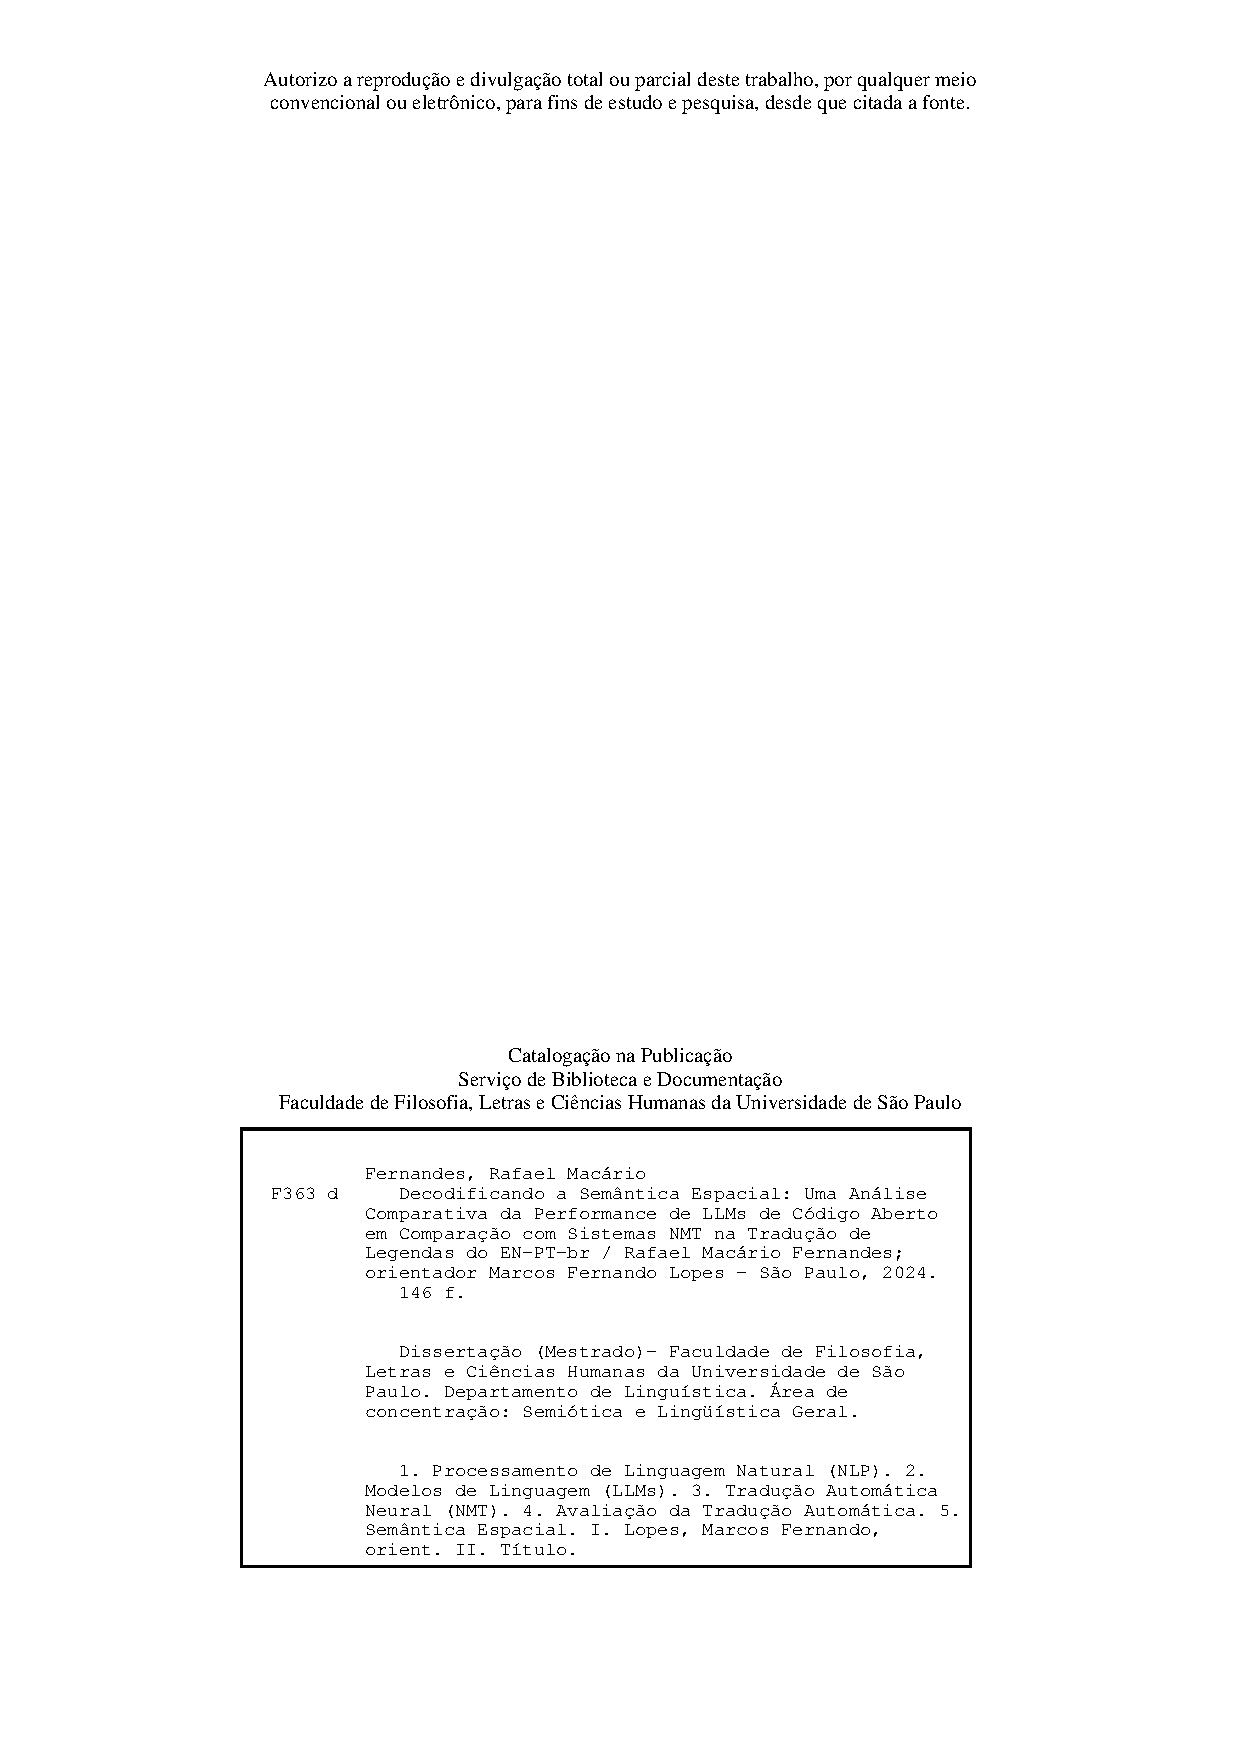
\includepdf{./figuras/file.pdf}
\clearpage

% Dedicatória (opcional)

~
\vfill
To my mother, my father, and my sister, for being my anchor.
\vfill

   
\clearpage

% Agradecimentos (opcional)
\chapter*{}



%% Insira aqui seus Agradecimentos. Não esqueça de mencionar as Agências
%% Financiadoras.

\vfill
\vfill
\vfill
O presente trabalho foi realizado com apoio da Coordenação de Aperfeiçoamento de Pessoal de Nível Superior - Brasil (CAPES) -- Código de Financiamento 001.

\bigskip 

\noindent This study was financed in part by the Coordenação de Aperfeiçoamento de Pessoal de Nível Superior -Brasil (CAPES) -- Finance Code 001.
\vfill
\clearpage

% Agradecimentos (opcional)
\chapter*{Acknowlegments}

%% Insira aqui seus Agradecimentos. Não esqueça de mencionar as Agências
%% Financiadoras.

\vfill

I want to start by thaking CAPES for funding my research and making this work possible. \\

My deepest gratitude goes to my advisor, Marcos Lopes, for his unwavering support and belief in me throughout the rollercoaster of my master's experience. Marcos, your steadfast patience, guidance, and encouragement have been my guiding lights. \\

I extend my heartfelt thanks to my former advisor, Cida Araújo, for introducing me to Cognitive Linguistics and Talmy's work on Spatial Semantics. This research would not have been possible without our collaboration on two invaluable PIBIC/CNPq projects during my undergraduate studies, which laid the groundwork for the work presented here. Cida, your teachings have been instrumental in shaping me into the researcher I am today. \\

To my comrads from the graduate program, you all know who you are. We have shared the highs and lows, frustrations and laughs, deadlines and memes, making this academic pursuit in Computational Linguistics a memorable one. \\

To my dear friends in São Paulo and Minas Gerais, you also know who you are. Your encouragement, support, and virtual presence have been a constant source of strength. \\

Last but not least, I would like to thank my family -- especially \textbf{my mother}. As the first in my family to study at a public university and pursue a graduate degree, achieving this milestone represents breaking a cycle of social injustice and fulfilling their unachieved dreams. Mom, thank you for always encouraging me to study and for helping me change my life through education.

\vfill
\clearpage

% Epígrafe (opcional)

~
\vfill
\begin{center}
    \begin{minipage}{8cm}
        %\begin{greek}
           The human mind is not, like ChatGPT and its ilk, a lumbering statistical engine for pattern matching, gorging on hundreds of terabytes of data and extrapolating the most likely conversational response or most probable answer to a scientific question. On the contrary, the human mind is a surprisingly efficient and even elegant system that operates with small amounts of information; it seeks not to infer brute correlations among data points but to create explanations.
        %\end{greek}
       
       \begin{flushright}
            --- Noam Chomsky on \textit{Artificial Intelligence} for The New York Times
        \end{flushright}
        
    \end{minipage}
\end{center}
\vfill

\clearpage

% Sumário
\abstractintoc
\tableofcontents*
\clearpage

\begin{brazil}
\begin{abstract}
\sloppy
\noindent \MakeUppercase{\Sobrenome}, \IniciaisDoNome ~\textit{\TítuloDoTrabalho.} \TipoTrabalho. Faculdade de Filosofia, Letras e Ciências Humanas, Universidade de São Paulo, \AnoDepósito.\\

\bigskip


% Insira aqui o seu resumo em português (em um único parágrafo de 150 a 500 palavras). Deve apresentar os objetivos, métodos, resultados e conclusões.
\noindent % Não tire esse comando dessa posição, colado ao texto.
Esta dissertação de mestrado investiga os desafios da tradução da espacialidade usando Grandes Modelos de Linguagem (LLMs) de código aberto em comparação com sistemas tradicionais de Tradução Automática Neural (NMT), abordando problemas na tradução de preposições espaciais como ACROSS, INTO, ONTO e THROUGH, que frequentemente são traduzidas utilizando-se formas verbais ou preposicionais semelhantes no português (EN-PT-br). A tradução correta dessas preposições é crucial para manter a integridade semântica da língua de origem, garantindo fluidez e aderência aos padrões de lexicalização da língua-alvo \parencite{house2018, talmy2000towardb, slobin2005relating}. A pesquisa contextualiza os desafios da tradução da linguagem espacial, destacando as limitações dos sistemas NMT atuais e as potenciais vantagens dos LLMs. A revisão de literatura traça a evolução das teorias de tradução, o desenvolvimento da NMT e o surgimento dos LLMs, descrevendo também suas limitações. A metodologia emprega uma análise baseada em corpus, a partir de um conjunto de dados bilíngue centrado em preposições espaciais de legendas de TED Talks obtidos pela plataforma OPUS. Este conjunto de dados foi meticulosamente pré-processado para facilitar tanto o cálculo de métricas automatizadas quanto a análise de erros manual. As métricas utilizadas incluem BLEU, METEOR, BERTScore, COMET e TER, enquanto a análise manual identifica e categoriza os tipos de erros que cada sistema comete. Os resultados revelam que LLMs de tamanho moderado, como LLaMa-3-8B e Mixtral-8x7B, alcançam precisão próxima aos sistemas NMT, como o Google, embora essa relação nem sempre seja linear, pois modelos como Gemma-7B possuíram desempenho similar na avaliação humana. No entanto, os LLMs em geral apresentaram sérios erros de tradução, incluindo interlíngua/code-switching (in) e anglicismos (an), não conseguindo transmitir idiomaticidade na língua-alvo. Por outro lado, os sistemas NMT alcançaram muito melhor fluidez na tarefa de tradução automática. No entanto, a análise humana destaca os desafios contínuos enfrentados tanto pelos LLMs quanto pelos sistemas NMT na tradução das nuances da espacialidade, com ambos os grupos apresentando números consistentes de erros como polissemia (po) e projeção sintática (sp), nos quais falham em traduzir o significado apropriado de uma preposição ou copiam os padrões de lexicalização da língua de origem para o texto alvo \parencite{fernandes-etal-2024-spatial, oliveira2022expressing}. A dissertação conclui que, apesar dos avanços nos LLMs, permanecem obstáculos na tradução precisa da linguagem espacial, sugerindo que pesquisas futuras devem se concentrar em aprimorar conjuntos de dados de treinamento, refinar arquiteturas desses modelos e desenvolver métricas de avaliação mais sofisticadas que capturem melhor as sutilezas da semântica espacial. Este estudo contribui para o campo fornecendo uma comparação detalhada do desempenho de LLMs e NMT na tradução da linguagem espacial do EN-PT-br, propondo direções para melhorias futuras.

\bigskip \noindent
\textbf{Palavras-chave:} \PalavrasChave .
\end{abstract}
\end{brazil}
\clearpage

% \addto{\captionsbrazil}{\renewcommand{\abstractname}{Abstract}}

%\begin{otherlanguage}{english}
\begin{english}
\begin{abstract}

\noindent \MakeUppercase{\Sobrenome}, \IniciaisDoNome ~ \textit{\TítuloEmIngles.} Dissertação de Mestrado. Faculdade de Filosofia, Letras e Ciências Humanas, Universidade de São Paulo, \AnoDepósito.\\

\bigskip
% Insira aqui o seu resumo em inglês (em um único parágrafo de 150 a 500 palavras). Deve apresentar os objetivos, métodos, resultados e conclusões.

\noindent % Não tire esse comando dessa posição, colado ao texto.
This master's thesis investigates the challenges of translating spatial language using open-source Large Language Models (LLMs) compared to traditional Neural Machine Translation (NMT) systems. It addresses the problem of accurately translating the semantics of spatial prepositions such as ACROSS, INTO, ONTO, and THROUGH, which are often translated into similar verbal or prepositional forms from English to Portuguese (EN-PT-br). Correctly translating these prepositions is crucial for maintaining the semantic integrity of the source content while ensuring fluency and adherence to the lexicalization patterns of the target language \parencite{house2018, talmy2000towardb,slobin2005relating}. The research begins by contextualizing the challenges of spatial language translation, highlighting the limitations of current NMT systems and the potential advantages of LLMs. A comprehensive literature review traces the evolution of translation theories, the development of NMT, and the rise of LLMs, while also describing the potential limitations of the current approach. The methodology employs a corpus-based analysis, assembling a bilingual dataset centered on spatial prepositions comprising TED Talks subtitles from the OPUS platform. This dataset was meticulously pre-processed to facilitate both automated metrics and manual error analysis. The evaluation metrics used include BLEU, METEOR, BERTScore, COMET, and TER, while the manual error analysis specifically identifies and categorizes the types of errors each system makes. The findings reveal that moderate-sized LLMs such as LLaMa-3-8B and Mixtral-8x7B achieve accuracy close to NMT systems such as Google, although this relationship is not always linear, as models like Gemma-7B presented similar performance in human reviews. However, LLMs generally presented other serious mistranslation errors, including interlanguage/code-switching (in) and anglicism (an) errors, failing to convey idiomacity in the target language. Conversely, NMT systems achieved better general fluency and precision for machine translation tasks. Manual error analysis, on the other hand, underscores the ongoing challenges both LLMs and NMT systems face in translating the nuances of spatial language, with both groups presenting consistent numbers of errors like polysemy (po) and syntactic projection (sp) errors, where they either fail to translate a preposition's appropriate meaning or copy the lexicalization patterns from the source text into the target text \parencite{fernandes-etal-2024-spatial, oliveira2022expressing}. The master's thesis concludes that despite the advancements in LLMs, significant hurdles remain in translating spatial language accurately. It suggests that future research should focus on enhancing training datasets, refining model architectures, and developing more sophisticated evaluation metrics that better capture the semantic subtleties of spatial language. This study contributes to the field by providing a detailed comparison of model performance in spatial language translation from EN-PT-br and proposing directions for future improvements.

\bigskip
\noindent \textbf{Keywords:} \Keywords
\end{abstract}
\end{english}



\clearpage

%\listofalgorithms
%\clearpage

\listoffigures
\clearpage

\listoftables
\clearpage

%%%%%%%%%%%%%%%%%%%%%%%%%%%%%%%%%%%%%%%%%%%%%%%%%%%
\mainmatter

\chapterstyle{madsen} % Algumas alternativas: ell; bianchi; demo2; veelo

    \pagestyle{companion}
    \OnehalfSpacing
    
    \chapter{Introduction}
\label{chapter:Introduction}

\epigraph{Thinking is a human feature. Will AI someday really think? That's like asking if submarines swim. If you call it swimming then robots will think, yes. \\ \hfill --- Noam Chomsky}

This Master's thesis investigates the complexities of using Neural Machine Translation (NMT) to translate spatial prepositions, particularly within the English-to-Brazilian Portuguese language pair. Through a comparative analysis, we investigate the effectiveness of Large Language Models (LLMs), also known as Generative AI (GenAI), against established NMT service providers like Google and DeepL. Specifically, our research explores how current open-source LLMs like Llama, Gemma, and Mistral handle the nuances of spatial language. We aim to discern these systems' capabilities in capturing the subtleties of translation in this domain, utilizing a corpus of TED Talks subtitles.

Imagine watching a captivating TED Talk where a speaker describes a scene using spatial language, only to have the subtitles completely miss the mark due to a mistranslated preposition or a poorly handled English phrase. For instance, if a man is described as ``struggling \emph{through}'' a dense crowd, the Portuguese subtitle might simply say ``se debatendo entre'' (floundering among), instead of the more idiomatic ``\emph{atravessando} com dificuldade,'' (crossing with difficulty), correctly emphasizing the aspect of moving past an obstacle conveyed by ``through'' in a verb root in Portuguese \parencite{Slobin-2004}. This highlights the growing need for high-quality translations in subtitles, particularly for capturing the nuances of spatial expressions. To address this challenge, while subtitling often relies heavily on human effort \parencite{karakanta-etal-2020-42}, this research explores the potential of using NMT, especially open-source LLMs, as an  solution.

This research evaluates the accuracy, fluency, and post-editing needs of LLMs compared to NMT systems and human translation, the gold standard. We employ a range of well-known evaluation metrics -- BLEU~\parencite{bleu}, METEOR~\parencite{lavie-agarwal-2007-meteor}, BERTscore~\parencite{zhang2020bertscore}, COMET~\parencite{rei-etal-2020-comet}, and TER~\parencite{snover-etal-2006-study} -- to assess content quality. By identifying potential strengths and weaknesses in handling spatial language, including polysemy, crosslinguistic differences, and other complexities, this research aims to contribute to both improved translation quality and the development of more effective evaluation methods in Machine Translation (MT).

TED Talks subtitles were particularly chosen because they perfectly combine semi-formal language with a closer approximation of everyday use. \textcite{Brysbaert2009} found that film and television subtitles are easy to gather, involve social interactions, and are more commonly watched than books are read. Their study on the psycholinguistic effect of word frequency measures showed that subtitle-derived frequencies significantly outperformed those from books and the internet. These findings highlight the value of using subtitles for linguistic research, ultimately influencing our decision.

\section{The Research Problem}

NMT has emerged as a significant advancement in Natural Language Processing (NLP), leveraging artificial neural networks to overcome the limitations of traditional methods that heavily relied on feature engineering. These systems, implemented through robust deep neural networks with multiple layers, can now learn intricate relationships between words and sequences~\parencite{TAN20205, wang-etal-2019-learning-deep}. Notably, the Transformer architecture, with its self-attention mechanisms, enables NMT to capture complex language structures, addressing the challenges previous statistical approaches faced in capturing long-distance dependencies within sentences~\parencite{vaswani2017attention, yang2020survey}.

Alternatively, the emergence of GenAI offers new possibilities for more natural and nuanced translations. Models like GPT (Generative Pre-trained Transformer) and BERT (Bidirectional Encoder Representations from Transformers) excel at understanding meaning across languages. They generate contextualized ``word embeddings'' that are sensitive to surrounding context, capturing subtle information within a sentence~\parencite{ethayarajh-2019-contextual}. However, accurately evaluating the quality of NMT remains challenging, particularly in contexts with ambiguity or where human references are lacking. This challenge is further amplified by the polysemy of spatial prepositions, whose meanings can vary significantly depending on the context~\parencite{bartsch-etal-2023-self, comsa2023benchmark, app11146584}.

Advances in language technology fuel research for better linguistic representations in NLP. However, complexities presented by the typological profiles of the world's languages and the expression of prepositional semantics across different language groups remain significant hurdles. As \textcite{oncevay-etal-2020-bridging} point out, the limited coverage of diverse training data creates a particular obstacle for integrating valuable resources like typology databases into NMT algorithms. Additionally, the inherent context-dependency of language, coupled with the specific challenges posed by spatial semantics -- including ambiguity caused by polysemy and abstractions in other domains -- impedes the construction of truly accurate and faithful models, as noted by \textcite[p.5]{herskovits1986language}. This knowledge gap can be partly attributed to the fact that benchmarks often exclude ambiguous instances from training datasets \parencite{Beigman-Klebanov2009}. This lack of real-world complexity during model training hinders these systems' abilities to manage the nuances encountered in real-world translation scenarios.

To illustrate this challenge, \textcite{fernandes-etal-2024-spatial} conducted a comparison of the performance of two prominent NMT systems, Google Translate (Google) and DeepL (DeepL), in translating the spatial scene in Example~\ref{ex:1} from the Cambridge Dictionary (CAM)\footnote{https://dictionary.cambridge.org/dictionary/english/} from English to Portuguese. For our study, we further translated the same sentence using two LLMs, OpenAI's GPT-3.5 (GPT-3.5) and Meta's LLaMa-3-7B (LLaMa-3), for comparison. A human translation by a professional translator served as a reference (REF). Additionally, we evaluated the translations using the following metrics: BLEU, METEOR, BERTScore, COMET, and TER.

\ex. He \colorbox{lightblue}{swam} \colorbox{lightgray}{\emph{across}} the river. (CAM) \label{ex:1} \\[0.3ex]
Ele \colorbox{lightgray}{\emph{\textcolor{ForestGreen}{atravessou}}} o rio \colorbox{lightblue}{\textcolor{ForestGreen}{nadando}}. (REF)\label{ex:1d} \\
$3$SG.M crossed the river by swimming. \\[-0.3ex] 
    \a. *~Ele \colorbox{lightblue}{\textcolor{Maroon}{nadou}} \colorbox{lightgray}{\emph{\textcolor{Maroon}{do outro lado}}} do rio. (Google) \label{ex:1a} \\
    $3$SG.M swam from-the other side of-the river.
    \b. Ele \colorbox{lightgray}{\emph{\textcolor{ForestGreen}{atravessou}}} o rio \colorbox{lightblue}{\textcolor{ForestGreen}{a nado}}. (DeepL) \label{ex:1b} \\
    $3$SG.M crossed the river by swimming.
    \c. *~Ele \colorbox{lightblue}{\textcolor{Maroon}{nadou}} \colorbox{lightgray}{\emph{\textcolor{Maroon}{através}}} do rio. (GPT-3.5) \label{ex:1c} \\
    $3$SG.M swam through-the river. 
    \d. ?~Ele \colorbox{lightblue}{\textcolor{Maroon}{nadou}} \colorbox{lightgray}{\emph{\textcolor{Maroon}{atravessado}}} o rio. (LLaMa-3) \\
    $3$SG.M swam crossed-the river. \\[0.3ex] \label{ex:1dd}

Example~\ref{ex:1} demonstrates the persistent difficulties encountered by NMT systems when dealing with issues such as language typology and preposition semantics. As observed, the translations provided by Google (``Ele nadou \emph{do outro lado d}o rio''), GPT-3.5 (``Ele nadou \emph{através d}o rio''), and LLaMa-3 (``Ele nadou \emph{atravessado} o rio), in \ref{ex:1a}, \ref{ex:1c}, and \ref{ex:1dd}, respectively, sound awkward, implying the swimmer moves either on an opposite bank or within the river's confines rather than crossing it entirely. In particular, translation \ref{ex:1dd} is not grammatically correct in Portuguese. When a participle form functions as a modifier in a verb phrase, it typically does not separate the verb and object, and is usually set off by a comma \parencite{cunha2016nova}. On the other hand, DeepL's rendition (``Ele \emph{atravessou} o rio a nado'') accurately captures the nuance of traversing the river perpendicularly, as seen in \ref{ex:1b}. This challenge stems from two reasons: the typologically different ways that English and Portuguese express motion and the polysemous meanings of the preposition ACROSS, which can signify both an opposite location and movement from one side to the other depending on the context \parencite{cambridge-across}. In this specific instance, the meaning is undeniably the latter. By analyzing such instances of mistranslations involving spatial language, we can gain valuable insights to enhance both the development and assessment methodologies for NMT systems.

\begin{table}[htb]
\small
  \centering
  \begin{tabular}{lccccc}
    \toprule
    & \multicolumn{5}{c}{\textbf{MT Metric}} \\
    \textbf{Model} & \textbf{BLEU} & \textbf{METEOR} & \textbf{BERTScore} & \textbf{COMET} & \textbf{TER} \\
    \midrule
    DeepL & $\mathbf{0.50}$ & $\mathbf{0.79}$ & $\mathbf{0.96}$ & $\mathbf{0.92}$ & $\mathbf{40.0}$ \\
    Google & $0.03$ & $0.24$ & $0.84$ & $0.74$ & $120.0$ \\
    GPT-3.5 & $0.05$ & $0.25$ & $0.87$ & $0.83$ & $80.0$ \\
    LLaMa-3 & $0.10$ & $0.52$ & $0.92$ & $0.86$ & $80.0$ \\
    \bottomrule
  \end{tabular}
\caption{MT Metrics for Translations in Example (1).}
\label{table:1.1}
\end{table}

In addition, while evaluation metrics can assess overall translation quality, they may struggle to evaluate the nuances of spatial relationships, as evidenced by Table~\ref{table:1.1}. In Example~\ref{ex:1}, Google, GPT-3.5, and LLaMa-3 misinterpret the correct meaning of ``ACROSS'', resulting in translation inconsistencies. However, despite these mistranslations, their unexpectedly high BERTScores ($0.84$, $0.87$, and $0.92$ respectively) and COMET scores ($0.74$, $0.83$, and $0.86$ respectively) raise questions about whether these more sophisticated metrics can effectively assess translation quality in cases like this, where language typology and polysemy issues are prevalent. The interesting observation is that if DeepL had not been included in the comparison, the next best translation choice would have been LLaMa-3 -- the second closest in meaning but grammatically incorrect sentence. Given their focus on overall semantic similarity, BERTScore and COMET might not specifically address these issues, which is precisely what explore in this study.

This gap becomes evident when comparing scores. While BERTScore and COMET, which focus on semantic similarity, overlook language typology and polysemy in spatial expressions, traditional metrics like BLEU (Google: $0.03$, GPT-3.5: $0.05$, and LLaMa-3: $0.10$) and METEOR (Google: $0.24$, GPT-3.5: $0.25$, and LLaMa-3: $0.52$) penalize the translations more due to their deviation from the reference in word order and synonyms. Lastly, unlike other metrics that measure text similarity, TER focuses on the number of edits needed to match the reference translation, indicating that DeepL's and Google's outputs would require $40$ and $120$ edits, respectively. This analysis emphasizes the dangers of underestimating each metric's strengths and weaknesses when evaluating the quality of translations involving spatial expressions, which, in some cases, can lead to misguided assessments and incorrect translation choices.


\section{Research Questions and Hypotheses}

This research aims to investigate the challenges of translating spatial expressions using LLMs compared to established NMT systems (henceforth sometimes both collectively referred to simply as ``models''), particularly focusing on their advantages and disadvantages compared to human translation. Our objective is to assess model performance when faced with issues such as language typology and prepositional semantics for the English-to-Brazilian-Portuguese (EN-PT-br) language pair.

In particular, we will analyze segments containing two preposition pairs that usually present challenges due to their overlapping meaning in PT-br: ACROSS and THROUGH, and INTO and ONTO (details will be discussed in Subsection~\ref{subsec: Challenges in Spatial Prepositions}).

To achieve this, our goal is two-fold:

\subsection{Analysis of Model Performance and Error Types}
\label{sub:q1-q2}

The first area focuses on analyzing model performance through the following questions:

\begin{itemize}
\item \textbf{Q1.} How do open-source LLMs compare against established NMT systems in terms of accuracy, fluency, and post-editing needs when translating segments with EN prepositions ACROSS, THROUGH, INTO, and ONTO from EN-PT-br? Are LLMs overall suitable for performing translation tasks for this specific language pair? 

\item \textbf{Q2.} Are spatial-related preposition errors, such as those involving syntactic projection (sp) and polysemy (po), among the most common in LLMs and NMT systems? Which prepositions and/or meanings are most frequently associated with these errors?
\end{itemize} 

Based on these questions, we propose the following hypotheses:

\newtcolorbox{hypothesis}{
colback=gray!5,
arc=4pt,
left skip=5pt,
right skip=5pt,
boxsep=5pt,
fonttitle=\bfseries,
boxrule = 0pt,
toprule = 4.5pt,
enhanced,
fuzzy shadow = {0pt}{-2pt}{-0.5pt}{0.5pt}{black!35},
width=\textwidth,
title=Hypothesis \#0 (Null):
}

\begin{hypothesis}
The quality of a translation does not differ significantly when considering whether a preposition is spatial or non-spatial.
\end{hypothesis}

\newtcolorbox{hypothesis2}{
colback=gray!5,
arc=4pt,
left skip=5pt,
right skip=5pt,
boxsep=5pt,
fonttitle=\bfseries,
boxrule = 0pt,
toprule = 4.5pt,
enhanced,
fuzzy shadow = {0pt}{-2pt}{-0.5pt}{0.5pt}{black!35},
width=\textwidth,
title=Hypothesis \#1 (Alternative):
}

\begin{hypothesis2}
The quality of a translation is influenced by whether a preposition is spatial or non-spatial, leading to significantly lower quality when it is spatial.
\end{hypothesis2}


For this analysis, we will utilize a human translated corpus of TED-Talk subtitles containing 2,000 segments (details will be discussed on Section~\ref{cap:Methods})

\subsection{Evaluation of MT Metrics}
\label{sub:q3-q4}

The second area of focus is the evaluation of automated MT metrics. We will investigate the effectiveness of these metrics in evaluating the accuracy of spatial language:

\begin{itemize}
    \item \textbf{Q3:} How effective are widely-used evaluation metrics BLEU, METEOR, TER, BERTscore, and COMET in capturing the accuracy and errors in translations containing the prepositions ACROSS, THROUGH, INTO, and ONTO from EN-PT-br? \label{Q3}
    \item \textbf{Q4:} What are the potential strengths and weaknesses of these metrics in identifying and assessing spatial-related errors such as syntactic projections (sp) and polysemy errors (po)? \label{Q4}
\end{itemize}

By investigating these questions, we aim to gain a deeper understanding of how well models handle spatial language in the context of automatic translation. Additionally, we can identify areas for improvement in both translation quality assessment (TQA) and translation quality estimation (TQE) to better capture the challenges and context-dependence of spatial prepositions.

\section{Motivation and Significance}

Accurate translations of spatial expressions are essential for conveying precise spatial relationships and preserving the meaning of the original text. However, NMT systems still struggle with this task due to the complexity of ``meaning, context, and world knowledge'' as highlighted by~\textcite[p.18]{house2018}. These systems often fail to capture subtle linguistic aspects like idioms, cultural connotations, and context-specific references.

Translating spatial expressions between EN-PT-br presents unique challenges due to how each language conveys spatial concepts. \textcite{fernandes-etal-2024-spatial} describe a phenomenon called ``an idiosyncratic projection of manner in verbs or adjuncts.'' This occurs because English has a richer vocabulary of verbs to express the manner of motion (e.g., run, sprint, dash) compared to Portuguese \parencite{Slobin-2004}. Consequently, NMT systems handling less common spatial expressions might directly translate the English verb's manner aspect into a Portuguese verb, even if that emphasis is atypical. This often results in awkward or inaccurate translations that lack idiomacity in the target language.

Furthermore, evaluating the quality of NMT systems, particularly for nuanced language features like spatial language, requires metrics that go beyond basic accuracy measures, such as word combinations and matching synonyms. While innovative BERT-based metrics can provide results comparable to human judgment, their true effectiveness remains unclear. These metrics are often assumed to model semantic similarity, but the underlying black-box nature of language model representations makes it difficult to fully understand how they arrive at their results \parencite{kaster-etal-2021-global}.


\section{The Approach}

This research employs a comparative approach, utilizing a classification scheme for error annotation based on established frameworks for analyzing MT errors \parencite{popovic-2018, Moorkens-2018} and classifying spatial semantics \parencite{talmy2000toward, talmy2000towardb, slobin2005relating}. This mixed methodology combines applied research aiming to evaluate the impact of spatial language on NMT, with both quantitative and qualitative methods. Model performance is measured through automated metric calculations and human evaluation. Our goal is to answer the proposed questions and to validate one of the two hypotheses.

By analyzing the performance of both LLMs and NMT systems on a carefully selected dataset containing sentences with two preposition pairs, we can assess their relative strengths and weaknesses in handling this linguistic challenge. Furthermore, we will evaluate the effectiveness of various automatic metrics in identifying and penalizing errors and inaccuracies in translations, with a particular focus on spatial-related errors.


\section{Expected Outcomes}

This study aims to provide a deeper understanding of the strengths and weaknesses of NMT systems, specifically through open-source LLMs, when handling spatial expressions. Our focus is on identifying common errors and potential patterns in how these systems translate spatial language. By uncovering these patterns, we hope to pave the way for future research that leverages LLMs to enhance the accuracy of open-source NMT systems, particularly for tasks like subtitling. This could lead to more precise and fluent translations across languages, facilitating better communication and comprehension.

Additionally, our analysis of MT evaluation metrics will highlight their limitations and suggest potential improvements for assessing translations involving complex language features, such as language typology and preposition polysemy. These findings can guide future research in both MT system development and evaluation metric design, ultimately leading to more nuanced and natural-sounding translations across languages.


\section{The Master's Thesis Structure} 

This master's thesis consists of several chapters, each devoted to specific aspects of translation and NMT evaluation, aimed at addressing the research questions and hypotheses.

Chapter \ref{cap:Literature}
conducts a comprehensive literature review, covering topics such as translation as intercultural communication, equivalence, subtitling challenges, and the role of technology. It also discusses challenges in spatial language translation and introduces NMT, highlighting its potential and limitations, along with the emergence of LLMs. Additionally, it explores automatic and manual methods for assessing translation quality.

Chapter \ref{cap:Methods} outlines the research methods, including corpus selection and compilation, data preprocessing, and the translation process using NMT systems and LLMs. It also describes the scoring methodology and data analysis techniques.

Chapter \ref{cap:Resultados} presents the research results and discussions, including outcomes of data cleaning, evaluation metrics across different models, and manual error analysis. It concludes by addressing research questions and hypotheses, with a focus on accuracy, fluency, and post-editing needs, particularly in spatial language translation.

Finally, Chapter \ref{cap:Conclusao} concludes the dissertation by summarizing the key findings, addressing limitations, and suggesting future research directions.





    \chapter{Literature Review}
\label{cap:Literature}

This chapter explores the multifaceted world of  translation. We start by examining translation as intercultural communication, exploring challenges like achieving equivalence in meaning and the unique demands of subtitling. We then address the limitations of human translation and the rise of technological solutions, like NMT systems and LLMs. Next, we focus on the specific challenge of translating spatial language, exploring spatial semantics (categories, patterns), the intricacies of English spatial prepositions, and the difficulties that arise when translating them between EN-PT-br. Finally, we conclude by examining methods for assessing translation quality, including human evaluation, manual error classification for spatial semantics, and automatic evaluation metrics.


\section{Translation as Intercultural Communication}

\epigraph{A language is not just words. It’s a culture, a tradition, a unification of a community, a whole history that creates what a community is. It’s all embodied in a language. \\ \hfill --- Noam Chomsky}

In our increasingly interconnected world, overcoming language barriers is crucial for fostering understanding and connection across cultures. Translation, the process of converting text from one language (source) to another (target), plays a vital role in this cross-cultural exchange. As noted by~\textcite[p. 9-10]{house2018}, it allows individuals from diverse backgrounds to access knowledge and experiences beyond their linguistic borders, enriching their understanding of the world through different perspectives.

However, translation goes beyond simply transfering linguistic content from a source text to a target text. It entails a series of complex cognitive processes that happens within the translator's brain, as well as a deep understanding of cultural interplay, as language, cognition, and culture are intricately linked. According to~\textcite{house2014translation}, every word and phrase carries not just its literal meaning but also cultural context, shaping how we view the world. This quote, from her book \enquote{Translation Quality Assessment: Past and present}, underscores the complex interplay between language, culture, and cognition in translation.


\begin{quote}
Language is culturally embedded: it serves to express and shape cultural reality, and the meanings of linguistic units can only be understood when considered together with the cultural contexts in which they arise, and in which they are used. In translation, therefore, not only two languages but also two cultures invariably come into contact. In this sense, then, translation is a form of intercultural communication. Over and above recognizing the importance of the two larger macro-cultural frameworks, however, the translator must of course also consider the more immediate ‘context of situation’. This more local situational context has to do with questions about who wrote the text, when, why, for whom, and who is now reading it, and for what purpose, etc. These questions, in turn, are reflected in how a text is written, interpreted, read and used. The context of situation is itself embedded in the larger socio-cultural world as it is depicted in the text and in the real world. \\
\phantom{abc} \hfill --- \textcite[4]{house2014translation}
\end{quote}

In that sense, translating effectively, as highlighted by~\textcite{house2014translation}, extends beyond conveying factual content. Translators navigate a challenging landscape, acting as bridges not only between languages but also the cultural contexts they embody. Beyond linguistic proficiency, they require critical situational judgment to understand the social and cultural environments of both source and target audiences. This balancing act demands ensuring the target text accurately reflects the intended meaning of the source language while faithfully representing its original message and cultural nuances~\parencite{house2018}. 

Achieving this balance becomes even more crucial in the current information age, marked by rapid technological advancements. While globalization has increased translation demand, it also intensifies the challenges of instant information flow and its reliance on English as a global lingua franca. The dominance of English, as noted by~\textcite[4]{house2014translation}, raises concerns about potential harm to language diversity and the diminished representation of diverse cultures in the global information flow.


\subsection{Translation and Equivalence}

Building upon the understanding that translation involves both cognitive processes and socio-cultural awareness, the concept of equivalence becomes crucial for achieving effective communication across cultures. 

While a literal translation might seem straightforward, it often falls short due to inherent differences between languages. \enquote{Equivalence}, unlike sameness or identity, focuses on conveying meaning with roughly equal value across these differences. Its Latin origin, meaning \enquote{of equal value,} emphasizes this core principle: acknowledging and working with the unavoidable differences between languages. As ~\textcite[6]{house2014translation} points out, this means preserving the intended meaning across different cultures.

\begin{quote}
The notion of equivalence is also related to the preservation of \enquote{meaning} across two different lingua-cultures. Three aspects of that meaning are particularly relevant for translation: a semantic aspect, a pragmatic aspect and a textual aspect. \\
\phantom{abc} \hfill --- \textcite[21]{house2014translation}
\end{quote}


The \textit{semantic meaning}, as explained by the author, focuses on the designated sense of words and their connection to the objects or ideas they represent. In contrast, \textit{pragmatic meaning} extends beyond the word level to include the speaker's intent, the communication context, and the impact on the listener. \textcite{house2014translation} highlights that pragmatic meaning emerges from the interaction between language, the speaker’s intention, the context, and the listener, contributing to the overall meaning-making process within a social setting.

The translation scholar further emphasizes this distinction by referencing a theorical work that helps us understand how utterances function beyond simply conveying information. The theory proposed by~\textcite{austin1962how, Searle1995-SEATCO}, known as speech act theory, introduces the concept of ``illocutionary force'', which essentially refers to the specific purpose or function of an expression in a particular context. This is distinct from the propositional content, which is the literal information conveyed. While grammatical features sometimes hint at the illocutionary force, \textcite[22]{house2014translation} clarifies that the context ultimately plays a crucial role in determining it in real-world situations.

Because translation deals with language in use, according to~\textcite[22]{house2014translation}, understanding the intended meaning and impact of a statement is crucial. Unlike dictionaries, for instance, which deal with isolated word meanings, translators work with complete units of communication (utterances) used in real-world situations. This means they consider not just the literal meaning of words (semantic meaning) but also the speaker's intent, the context, and the desired effect on the listener (pragmatic meaning). The author acknowledges that, sometimes, prioritizing the intended message and impact might require sacrificing some degree of literal meaning. Imagine trying to translate a joke – focusing solely on word-for-word accuracy might miss the humor entirely. In such cases, the translator aims for functional equivalence, ensuring the translated message conveys the original intent and effect even if the wording differs slightly.

Finally, the last aspect, \textit{textual meaning}, is another crucial element for achieving equivalence in translation, as emphasized by~\textcite[22-23]{house2014translation}. A text, the author explains, is any stretch of language where its individual components are interconnected and form a cohesive whole. Think of it like a paragraph or longer passage where sentences work together to convey a larger meaning. Various relationships within the text, such as theme progressions, pronouns, substitutions, and references, contribute to the overall textual meaning that needs to be considered during translation \parencite{house2014translation}.

With that in mind, achieving effective cross-cultural communication through translation necessitates a nuanced approach that goes beyond simply matching words from one language to another. Equivalence, acknowledging and working with the inherent differences between languages, is key to preserving the intended meaning across cultures. As we move forward, understanding the complexities of equivalence will remain central to fostering effective communication in our increasingly interconnected world.


\subsection{Subtitling and its Unique Challenges}

The global landscape of entertainment has shifted dramatically. The rise of streaming platforms have fueled a surge in demand for accessible multilingual content. Movies, TV shows, documentaries, and other audiovisual media are now translated into numerous languages to cater to diverse audiences. This abundance of translated content highlights the critical importance of providing accurate and culturally nuanced translations.

In this context, \emph{subtitling}, the process of displaying translated text synced with the audio, plays an important role. It fosters cultural exchange by allowing non-native speakers to access and understand foreign media. However, subtitling presents a unique set of challenges distinct from traditional written translation. As translation scholars \textcite{cintas2020subtitling} point out, subtitling goes beyond simply translating spoken words. It encompasses various elements of the audiovisual experience:

\begin{quote}
(Subtitling) may be defined as a translation practice that consists in presenting a written text, generally on the lower part of the screen, that aims to recount the original dialogue exchanged among the various speakers, as well as all the other verbal information that is transmitted visually (letters, inserts, graffiti, text messages, inscriptions, placards, and the like) and orally (songs, voices of, voiceover narration). \\
\phantom{abc} \hfill --- \textcite[9]{cintas2020subtitling}
\end{quote}

This multifaceted nature, as highlighted above, presents unique challenges distinct from traditional written translation, as \textcite{cintas2020subtitling} further explain:

\begin{quote}
All subtitled programmes are made up of three main constituents: the spoken word, the image and the subtitles. The interaction of these three components, along with the viewer’s ability to read both the images and the written text at a particular speed, and the actual size of the screen, determine the basic characteristics of the audiovisual medium. Subtitles must appear in synchrony with the images and dialogue, provide a semantically adequate account of the SL (source language) dialogues, and remain displayed on screen long enough for the viewers to be able to read them. \\
\phantom{abc}
\hfill --- \textcite[9]{cintas2020subtitling}
\end{quote}

These complexities, as outlined in the second quote, contribute to the specific challenges faced by subtitlers. Unlike written text, subtitles are constrained by limited space and the need to synchronize with both the speaker's pace and the viewer's reading speed. Additionally, conveying cultural references and technical vocabulary within these time constraints demands creative solutions~\parencite{matusov-etal-2019-customizing}. Subtitlers must therefore possess a diverse skill set, including proficiency in both languages, excellent writing skills, cultural sensitivity, and the ability to condense meaning while maintaining clarity and accuracy~\parencite{cintas2020subtitling}.

In this master's thesis research, due to time constraints, we will treat the segments in our subtitle corpus as complete spoken utterances. This approach temporarily sets aside the limitations inherent to subtitling, such as screen time limits and character restrictions. For example, consider a complex spatial expression conveyed in a long sentence, such as ``The bird flew down from out of the hole in the tree and onto the little girl's face as she walked along the sidewalk. '' In subtitling, this sentence might be split into multiple lines due to character limits, potentially losing the nuances and complexity of the original expression. By simplifying the analysis in this way, we focus on investigating the linguistic phenomenon at hand and establish a foundation for further research, which will allow us to address subtitling constraints in future studies.


\subsection{Human Translation: Current Limitations and the Need for Technological Solutions}

Throughout history, human translation has been pivotal in various aspects of human development. It has facilitated the invention and spread of writing systems, fostered the formation of national languages and literatures, and enabled the exchange of knowledge, political power, and cultural influences across borders. According to \textcite{house2014translation}, human translation has been invaluable in various domains, from diplomatic negotiations to scientific collaborations and the dissemination of religions and cultural values.

Even in the modern world, human translators' deep cultural and linguistic knowledge uniquely equips them to capture the nuances, cultural references, idioms, and context of the source language, enabling them to deliver high-quality translations ~\parencite{dalayli-2023-use}.

Nevertheless, human translation faces challenges in \emph{scalability}. Individual limitations in capacity and time, coupled with the often-necessary research to ensure the quality of the traslated texts, can hinder its effectiveness in large-scale projects. As highlighted by \textcite{kenny2022human} in her paper ``Human and Machine Translation,'' time-consuming research is frequently needed when translators encounter difficulties understanding the source text, recalling specific terminology, or formulating ideas in the target language:

\begin{quote}
When a professional translator does not understand something in the source text, or cannot recall a specialized term in the target language, or is struggling to come up with a way of formulating an idea in the target language, she will usually divert her attention from the text at hand, and do some research. A translator grappling with the niceties of wastewater treatment, for example, may go to the website of various local authorities to see how they explain the technology involved. She might access one of the many publicly available termbanks to find an equivalent for a given term. She might consult other documentation produced by her client’s company or speak to engineers at the company. \\
\phantom{abc} 
\hfill --- \textcite[29]{kenny2022human}
\end{quote}

This research-intensive process, while crucial for maintaining translation quality, emphasizes the scalability limitations of human translation. As \textcite{kenny2022human} further details, translators may encounter specialized fields or poorly written source texts requiring additional effort and expertise beyond their immediate domain:

\begin{quote}
Even experienced translators will sometimes admit to difficulty in translating texts that are highly technical and for which they lack sufficient training. Whereas a translator with an educational or professional background in legal studies or practice might relish working on the translation of legislation, a specialist in automotive engineering will run (or drive) a mile from such work. It can also happen that, even within their own domain, translators can come across source texts that are badly written, or incomplete, or written in a way that makes them extremely difficult to understand. \\
\phantom{abc}
\hfill --- \textcite[29]{kenny2022human}
\end{quote}

While specialization equips translators to handle complex texts, it necessitates constant upskilling and increases \emph{costs}, further hindering scalability, particularly for smaller projects where human translation is cost-prohibitive. These limitations pave the way for the exploration of technological solutions alongside human expertise. As a result, MT has emerged as a powerful tool, widely adopted across various translation fields, due to its suitability for large-scale applications and cost-effectiveness for specific content types  \parencite{karakanta-etal-2020-42}. As emphasized by \textcite{kenny2022human}:

\begin{quote}
The use of MT in translation production does not necessarily entail a loss of quality, and the cost and effort of human translation is not appropriate for all types of texts, particularly those with a short shelf-life that present little risk. \\
\phantom{abc} \hfill --- \textcite[129-130]{kenny2022human}
\end{quote}

For \textcite{kenny2022human}, the use of MT can be particularly beneficial in scenarios where human translation costs or turnaround times are limited. This supports the notion that MT is not meant to replace human translators entirely, but rather complement their expertise in situations where its strengths are best suited. That said, it is important to acknowledge that MT is still under development. Its ability to handle the complexities of audiovisual translation (AVT) and creative texts, for instance, remains limited due to the inherent challenges in understanding these specific content types \parencite{Burchardt2016}.

Therefore, in the quest for effective translation solutions, a hybrid approach that combines the strengths of both human and machine translation is gaining prominence. By leveraging human expertise for tasks requiring creativity, cultural understanding, and domain-specific knowledge, and utilizing MT for routine or large-scale projects, this hybrid approach achieves both scalability and cost-effectiveness while preserving quality.

This evolving landscape requires adaptation from practicing translators. Their roles are transforming towards \emph{post-editing} tasks, as highlighted by Robert Lane Greene in The Economist's Technology Quarterly on Language:

\begin{quote}
The ‘translator’ of the future is likely to be more like a quality control expert, deciding which texts need the most attention to detail and editing the output of MT software. That may be necessary because computers, no matter how sophisticated they have become, cannot yet truly grasp what a text means.\\
\phantom{abc} \hfill --- \textcite{economist2017}
\end{quote}

All in all, despite its historical importance, human translation faces limitations in scalability and cost in the modern world, necessitating alternative solutions. While MT offers advantages in these areas, its ongoing development means it struggles with complexities like audiovisual translation and creative texts. The future, therefore, lies in a collaborative approach, where human expertise tackles nuances and complexities while MT handles routine tasks. This synergy between humans and machines paves the way for efficient, cost-effective, and high-quality translations, fostering communication across languages in a globalized world.


\section{Translating Spatial Language}
\label{sec: translating-spatial}

\epigraph{Language is not just a tool for communication; it is also a tool for thought. Our language shapes the way we think and the ideas we can conceive. \\ \hfill --- George Lakoff}

The study of spatial expressions, that is, the diverse ways through which we use language to convey motion, location, and spatial relationships between objects, has become a significant field of research across various disciplines \parencite{levinson2006grammars}. This growing interest stems from the crucial role spatial language play in diverse fields like Cognitive Linguistics~\parencite{LakoffJohnson80, talmy1985lexicalization, talmy2000toward, talmy2000towardb, oliveira2022expressing}, Cognitive Psychology~\parencite{slobin1985crosslinguistic, slobin1987thinking, slobin1996thought, slobin2005relating, taylor1996perspective,  tversky2003structures, oliveira2021hipotese}, Semantics~\parencite{zwarts2016counterdirectionality}, Natural Language Processing~\parencite{dobnik2018exploring, ghanimifard2019neural, kelleher2022distributional}, and Artificial Intelligence~\parencite{gotts1996connection, ligozat2007language, zang2018translating, rodrigues2017pinning, rodrigues2020standpoint}.

Despite its undeniable importance, defining the exact scope of spatial language remains a multifaceted challenge due to its interdisciplinary nature. \textcite{zlatev-spatial} emphasizes that the spatial domain is not easily delineated and often overlaps with other types of meaning, complicating efforts to establish clear boundaries. Furthermore, in Cognitive Linguistics, space is frequently used metaphorically to represent abstract concepts, such as time (e.g., ``I'll arrive \emph{on} time''), emotions (e.g., ``She's \emph{in} love''), and idiomatic expressions (e.g., ``He's feeling \emph{under} the weather'') \parencite{ coventry:04b}. This metaphorical use of space reflects how spatial relationships extend beyond physical dimensions to encompass how humans conceptualize and organize abstract ideas based on their bodily experiences. Thus, space functions both as a literal and metaphorical framework, influencing how we understand and convey spatial relationships and concepts.

However, despite these complexities, this section aims to explore the nuances involved in translating spatial expressions for the EN-PT-br pair. We will examine how different parts of speech lexicalize spatial meanings in the two languages, before ultimately focusing our attention on prepositions ACROSS, THROUGH, INTO, and ONTO.


\subsection{Spatial Semantics: Categories and Lexicalization Patterns} 

This section explores the complexities involved in translating ``Motion Events'' across languages. While numerous fundamental categories have been proposed in the literature, a comprehensive analysis can be a challenging task. Therefore, this study adopts the semantic concepts of \emph{Figure}, \emph{Ground}, \emph{Motion}, \emph{Path}, \emph{Manner}, and \emph{Cause} \parencite{talmy1985lexicalization, talmy2000toward, talmy2000towardb}. These terms, though not all universally adopted, align well with our chosen approach, despite minor variations in different research perspectives.


\subsubsection{The Semantic Components of Motion Events} 

The basic ``Motion event'', as defined by \textcite[25-26]{talmy2000towardb}, involves a single object (the Figure) located or moving relative to another object (the reference object, or Ground) in either \emph{self-contained} or \emph{translational motion}. The first type refers to motion without a change of location in space, such as rotation, oscillation, or dilation, while the latter involves the Figure’s location changing over time \parencite{shan2018review}. This concept is broken down into four essential components: 

\begin{itemize}
  \item \emph{Figure} (F): The object moving or in static location.
  \item \emph{Ground} (G): The reference object serving as a point of comparison.
  \item \emph{Path} (P): The path taken by the Figure in relation to the Ground (when moving) or its fixed location (when static).
  \item \emph{Motion}: The state of the Figure --- either moving (MOVE) or stationary (BE\begin{scriptsize}LOC\end{scriptsize}).
\end{itemize}

In addition to the four core components, Motion events can be accompanied by an external element called ``Co-event'', typically expressing the Manner (M) and/or Cause (C) of the motion. These additional elements, as well as the essential four described above, can be observed in Examples~\ref{ex:2}, \ref{ex:3}, \ref{ex:4}, and \ref{ex:5} adapted from \textcite{talmy2000towardb}. 
Figure~\ref{fig:patterns-events} summarizes the semantic schema of Motion events.

\footnotesize{
\ex. MOVE + Manner: \label{ex:2}
    \a. The rock\begin{scriptsize}$<$F$>$\end{scriptsize} \textbf{rolled}\begin{scriptsize}$<$MOVE + M$>$\end{scriptsize} \textit{down}\begin{scriptsize}$<$P$>$\end{scriptsize} the hill\begin{scriptsize}$<$G$>$\end{scriptsize}. $=$ 
    [the rock MOVED down the hill] WITH-THE-MANNER-OF [the rock rolled] 
    \b. The gate\begin{scriptsize}$<$F$>$\end{scriptsize} \textbf{swung}\begin{scriptsize}$<$MOVE + M$>$\end{scriptsize} shut \textit{on}\begin{scriptsize}$<$P$>$\end{scriptsize} its rusty hinges\begin{scriptsize}$<$G$>$\end{scriptsize}. $=$ [the gate MOVED shut ($=$ the gate shut)] WITH-THE-MANNER-OF [the gate swung on its rusty hinges] 

\ex. MOVE + Cause: \label{ex:3}
    \a. The napkin\begin{scriptsize}$<$F$>$\end{scriptsize} \textbf{blew}\begin{scriptsize}$<$MOVE + C$>$\end{scriptsize} \textit{off}\begin{scriptsize}$<$P$>$\end{scriptsize} the table\begin{scriptsize}$<$G$>$\end{scriptsize}. $=$ 
    [the napkin MOVED off the table] WITH-THE-CAUSE-OF [(something) blew on the napkin] 
    \b. The man \textbf{hammered}\begin{scriptsize}$<$MOVE + C$>$\end{scriptsize} the nail\begin{scriptsize}$<$F$>$\end{scriptsize}  \textit{into}\begin{scriptsize}$<$P$>$\end{scriptsize} the board\begin{scriptsize}$<$G$>$\end{scriptsize} with a mallet. $=$ [the man MOVED the nail into the board] WITH-THE-CAUSE-OF [he hammered it with a mallet] 
    
\ex. BE\begin{scriptsize}LOC\end{scriptsize} + Manner: \label{ex:4}
    \a. The lamp\begin{scriptsize}$<$F$>$\end{scriptsize} \textbf{stood}\begin{scriptsize}$<$BE\begin{scriptsize}LOC\end{scriptsize} + M$>$\end{scriptsize} \textit{on}\begin{scriptsize}$<$P$>$\end{scriptsize} the table\begin{scriptsize}$<$G$>$\end{scriptsize}. $=$ [the lamp BE\begin{scriptsize}LOC\end{scriptsize} on the table] WITH-THE-MANNER-OF [it stood there]
    \b. The rope\begin{scriptsize}$<$F$>$\end{scriptsize} \textbf{hung}\begin{scriptsize}$<$BE\begin{scriptsize}LOC\end{scriptsize} + M$>$\end{scriptsize} \textit{across}\begin{scriptsize}$<$P$>$\end{scriptsize} the canyon\begin{scriptsize}$<$G$>$\end{scriptsize} from two hooks. $=$ [the rope BE\begin{scriptsize}LOC\end{scriptsize} across the cannyon] WITH-THE-MANNER-OF [it hung there]

\ex. BE\begin{scriptsize}LOC\end{scriptsize} + Cause: \label{ex:5}
    \a. The pencil\begin{scriptsize}$<$F$>$\end{scriptsize} \textbf{stuck}\begin{scriptsize}$<$BE\begin{scriptsize}LOC\end{scriptsize} + M$>$\end{scriptsize} \textit{on}\begin{scriptsize}$<$P$>$\end{scriptsize} the table\begin{scriptsize}$<$G$>$\end{scriptsize} (after I glued it). $=$ [the pencil BE\begin{scriptsize}LOC\end{scriptsize} on the table] WITH-THE-MANNER-OF [it stuck there (after I glued it)]


\normalsize{

\begin{figure}[htb]
\centering
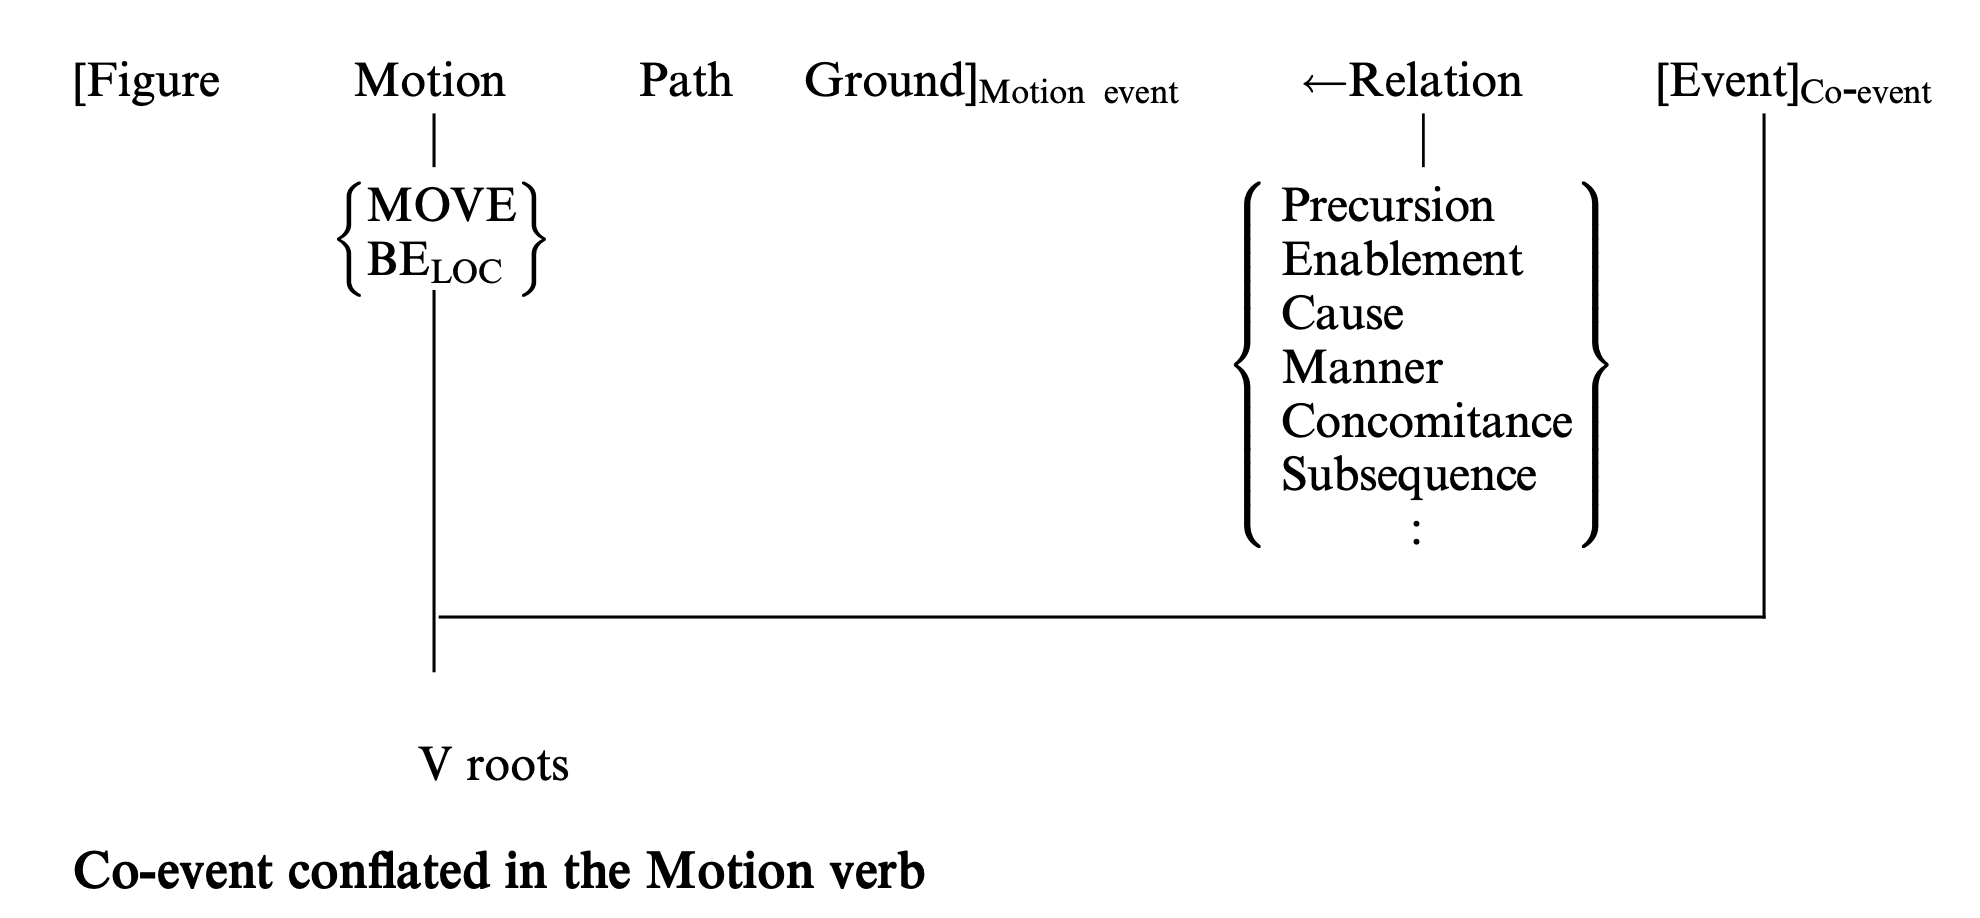
\includegraphics[width=0.8\textwidth]{figuras/Screen Shot 2024-05-17 at 13.01.00.png}
\caption{\label{fig:patterns-events} Patterns in Representation of Event Structure  \parencite[28]{talmy2000towardb}.}
\end{figure}


\subsubsection{Meaning and Form in Language}

\textcite[21]{talmy2000towardb} argues for a systematic connection between \textit{meaning} and \textit{form} in language. Semantic concepts (like \emph{Figure}, \emph{Ground} and \emph{Motion}) represent the linguistic meanings. Surface expressions, on the other hand, represent the various grammatical forms used to convey these meanings, such as verbs, adpositions, subordinate clauses, and \emph{satellites}. The latter are defined as closed-class elements like prepositions and adverbials that have a ``sister relation" to verbs and other phrases \parencite{oliveira2022expressing}.
 
\begin{quote}
A combination of semantic elements can be expressed by a single surface element, or a single semantic element by a combination of surface elements. Or again, semantic elements of different types can be expressed by the same type of surface element, as well as the same type by several different ones. We find here a range of universal principles and typological patterns as well as forms of diachronic category shift or maintenance across the typological patterns. \\
\phantom{abc}
\hfill --- \textcite{talmy2000towardb}
\end{quote}

Understanding this intricate relationship between meaning and form is crucial for an accurate translation. \textcite{talmy2000towardb}'s observation highlights the multifaceted nature of this connection. A single semantic element, like Manner, can be conveyed through various surface forms depending on the language (e.g. the verb ``to struggle'' in English can be expressed by ``debater-se'' (to flounder), ``tentar duramente'' (try hard)  ou ``fazer um grande esforço'' (make a big effort) in Portuguese, that is, through a verb, a verb-adverb combination, or even a complex clause). Conversely, the same surface form in one language might encode different semantic elements in another. For instance, the English preposition ``into,'' used to convey the Path element with directionality, might require a combination of surface forms like ``entrar em/dentro de'' (go into) in Portuguese.

However, it is important to recognize that even skilled human translators may not always have explicit linguistic awareness of these nuances. High-quality translation often relies on an intuitive grasp of language and context rather than a detailed, conscious understanding of linguistic theory. Therefore, while translators may effectively handle these challenges in practice, the theoretical complexity of meaning and form highlights the importance of developing and refining automated translation systems to bridge potential gaps in linguistic knowledge and achieve more nuanced and accurate translations.

\subsubsection{The Spatial Domain: from Language Typology to Neo-determinism}

Based on a systematic observation of universal and typological features across human languages, \textcite{talmy2000towardb} proposes a two-fold typological classification of language groups. The first group, \texttt{satellite-framed} languages, primarily express Motion and Co-events (Cause or Manner) through a single verb root (e.g., to run, to crawl, to climb). They also have a smaller set of verbs to express static location with these additional elements. The Path component, on the other hand, is generally expressed in a satellite (e.g. prepositions). English, as well as other Germanic languages, such as German and Dutch, and most Indo-European languages (except Romance) are a part of this group. 

In contrast, \texttt{verb-framed} languages typically separate Motion from Co-events. Their verbs primarily encode the Path element (e.g., enter, pass, exit), while Manner or Cause are expressed with separate words like adverbs, gerunds, or prepositional phrases. Romance languages like Portuguese and Spanish, Semitic languages, Basque, Korean, and Japanese fall into this category. Figure~\ref{fig:s-v-distinction} visually summarizes this distinction, and Examples~\ref{ex:5a} and~\ref{ex:5b} from \textcite{oliveira2022expressing}, further illustrate the two groups.

\begin{figure}[htb]
\centering
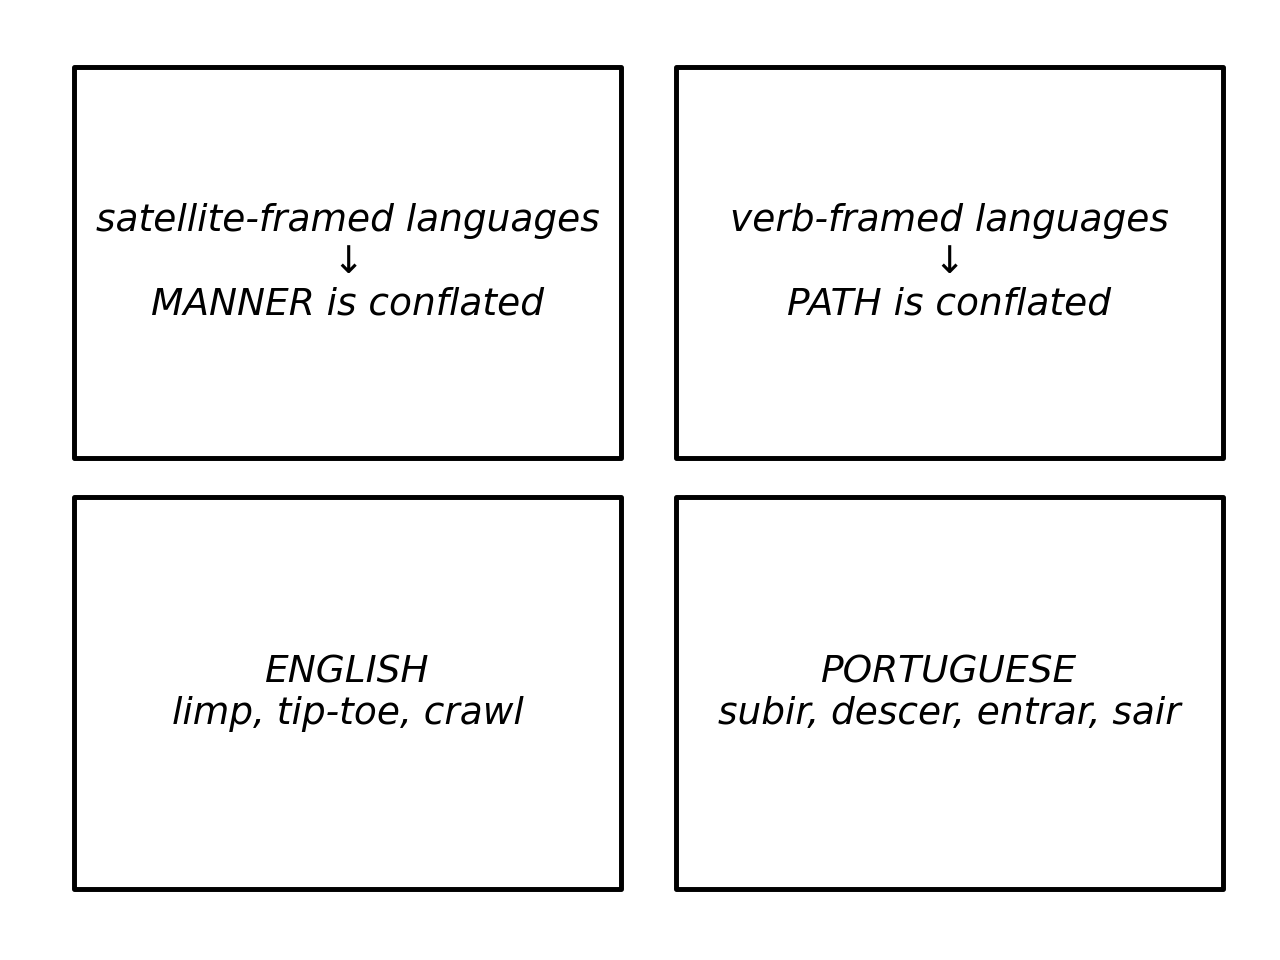
\includegraphics[width=0.7\textwidth]{figuras/Unknown-4.png}
\caption{\label{fig:s-v-distinction} Distinction between English (\texttt{satellite-framed}) and Portuguese (\texttt{verb-framed}) (Source: our own).}
\end{figure}

\ex. 
    \a. The pencil \textbf{rolled}\begin{scriptsize}$<$M$>$\end{scriptsize} \textit{off}\begin{scriptsize}$<$P$>$\end{scriptsize} the table. \\
    \emph{O lápis \textit{saiu}}\begin{scriptsize}$<$P$>$\end{scriptsize} \textbf{\emph{rolando}}\begin{scriptsize}$<$M$>$\end{scriptsize} (e caiu) \emph{da mesa}. \label{ex:5a} 
    \b. The boy \textbf{stepped}\begin{scriptsize}$<$M$>$\end{scriptsize} \emph{aside}\begin{scriptsize}$<$P$>$\end{scriptsize}. \\
    \emph{O garoto se \textit{afastou}}\begin{scriptsize}$<$P$>$\end{scriptsize}. \label{ex:5b}

Interestingly, English commonly uses multiple prepositions to indicate the \emph{trajectory} (or complex path) of a Figure in motion. As \textcite{oliveira2022expressing} point out, this is also why it is very common to find descriptions containing multiple prepositions that indicate the subgoals of a Figure, as shown in Example~\ref{ex:6}.

\ex. 
    The frog \textbf{crawled} \textit{out of} the jar\begin{scriptsize}$<$1$>$\end{scriptsize} and \textit{through} the window\begin{scriptsize}$<$2$>$\end{scriptsize} \textit{into} the woods\begin{scriptsize}$<$3$>$\end{scriptsize}. \label{ex:6} 
    \emph{O sapo escapou} \textbf{sorrateiramente} \emph{da jarra, saiu pela janela e fugiu para a floresta.}


The translation of Example~\ref{ex:6}  illustrates a challenging real-world scenario where the translator prioritizes idiomacity in the target language over original semantic nuances. For instance, ``crawled out of'' is translated as ``escapou sorrateiramente'' (slyly escaped), shifting the focus from the Manner of motion to the outcome of escaping. A more literal translation, such as ``o sapo rastejou para fora,'' would preserve the Manner aspect but would sound less idiomatic in Portuguese. Similarly, ``through the window'' and ``into the woods'' are translated as ``saiu pela janela' and ``fugiu para a floresta,'' emphasizing \emph{changes of state} rather than motion dynamics. In \texttt{verb-framed} languages, such as Portuguese, Manner verbs like ``crawl'' are generally avoided when describing events that involve crossing boundaries due to a ``boundary-crossing constraint,'' where the main verb typically encodes the change of state rather than the activity (Manner of motion), as described by~\textcite{Slobin2006WhatMM}. Exceptions include high-energy, punctual acts that can be conceptualized as a change of state, like ``throw oneself,'' but generally, Manner verbs are incompatible with describing activities extended in time or space across boundaries.

These typological differences raise intriguing questions about the relationship between language and thought. Does language merely reflect our conceptualization of the world, or does it play a more active role in shaping it? This line of inquiry delves into the realm of neo-determinism, which builds upon the classic Sapir-Whorf hypothesis. This theory, as discussed by~\textcite{cadierno2017thinking}, proposes a strong link between language and thought, suggesting that language structures influence how we perceive the world. While this extreme view might be debatable, Slobin's ``thinking for speaking'' hypothesis \parencite{slobin1996thought, Slobin-2004, slobin2005relating} offers a more nuanced perspective on the matter.

\textcite{slobin1987thinking} argues that language acts as a tool during speech production. We do not simply translate a pre-existing ``mental image'' into words. Instead, the grammatical resources available in our language influence the specific details we choose to focus on and encode within an utterance. The passage quoted below highlights this concept:

\begin{quote}
A particular utterance is never a direct reflection of ``objective'' or perceived reality or of an inevitable and universal mental representation of a situation. This is evident within any given language, because the same situation can be described in different ways; and it is evident across languages, because each language provides a limited set of options for the grammatical encoding of characteristics of objects and events. ``Thinking for speaking'' involves picking those characteristics that (a) fit some conceptualization of the event, and (b) are readily encodable in the language. \\
\phantom{abc}
\hfill --- \textcite[435]{slobin1987thinking}
\end{quote}

According to~\textcite{slobin1987thinking}, refined semantic elements such as aspect, definiteness, manner of movement, and point of view might not be easily conflated in all languages. In addition, Talmy's typology, as discussed earlier, provides valuable insights into this cross-linguistic variation in how languages encode motion events. Therefore, in essence, ``thinking for speaking'' involves selecting aspects of an event that are both conceptually relevant and readily expressible within the constraints of a particular language.

In translation, understanding language typology and neo-determinism is key to navigating cross-linguistic differences. Talmy’s typology shows that languages like English and Portuguese use different strategies for expressing motion: English typically encodes path in satellites, while Portuguese incorporates it into verb roots. Slobin's concept of ``thinking for speaking'' further explains that languages prioritize different elements -- Manner in English and Path in Portuguese -- which impacts translation practices. In fact, studies such as \textcite{cifuentes-ferez2015thinking, alonso2022} examine strategies like omission and replacement for Path verbs when translating from French to Galician and English, and Manner verbs from English to Spanish. Findings from \textcite{cifuentes-ferez2015thinking} reveal that typological differences and translator expertise significantly influence translation strategies. Consequently, as MT systems advance, incorporating this linguistic knowledge is paramount to enhancing translation quality and preserving the intended meaning when translating in the spatial domain.


\subsection{The Semantics of English Spatial Prepositions}
\label{sec: Spatial Prepositions}

As briefly discussed in Section~\ref{sec: translating-spatial}, within the framework of Cognitive Linguistics, the domain of space has been widely regarded as a fundamental tool for the structuring of other conceptualized domains through an extensive use of metaphorical language \parencite{LakoffJohnson80}. For instance, as noted by~\textcite{coventry:04b}, spatial prepositions frequently occur in the domains of time (e.g., ``I'll arrive in five minutes''%M: Os exemplos citados diretamente no meio do texto cursivo deveriam vir entre aspas. Os que estão no ambiente \ex. podem ficar como estão. 
%R: Feito.
), emotions (e.g., ``I'm feeling down today''), and idiomatic expressions (e.g., ``I'm in a hurry''). 

Spatial prepositions also frequently exhibit polysemy, that is, they present distinct but related senses, which, in certain translation contexts, may result in ambiguity. According to~\textcite{coventry:04b}, although English prepositions can express information about a Path (the specific way a Figure moves through space), the type of path is often determined by the verb used, such as illustrated in Example~\ref{ex: over-1} and \ref{ex: over-2}. 

\ex. 
    \a. Kathryn walks \textit{over}\begin{scriptsize}$<$P-direction$>$\end{scriptsize}\label{ex: over-1} the hill. 
    \b. Kathryn lives \textit{over}\begin{scriptsize}$<$P-location$>$\end{scriptsize}\label{ex: over-2} the hill.

In \ref{ex: over-1}, \textcite{coventry:04b} explains how ``over'' indicates the Path in relation to a reference object (the hill) -- Kathryn is likely following a path up and down the hill. On he other hand, in \ref{ex: over-2}, ``over'' refers to Kathryn's location on the opposite side of the hill, which is a different position relative to the speaker's current location. Therefore, despite using the same preposition, these sentences convey different spatial relationships.

While this subsection briefly mentioned some uses in different domains, its focus is on describing the polysemous spatial meanings associated with four directional prepositions: ACROSS, THROUGH, INTO, and ONTO. \textcite{bruckfield2011prepositions} distinguishes these first two prepositions from the last two, stating that the first group (ACROSS and THROUGH) does not necessarily imply reaching a destination on the other side of something. To achieve this goal, we will analyze the book ``Prepositions: The Ultimate Book - Mastering English Prepositions''\parencite{bruckfield2011prepositions} and the Cambridge  Dictionary (CAM) to compile a list of spatial meanings and some metaphorical uses, illustrating them with examples.


\subsubsection{The Preposition ACROSS}

The basic idea of ACROSS is to indicate movement or position over the surface or extent of something. It typically applies to two-dimensional spaces \parencite{bruckfield2011prepositions}. While ACROSS can imply movement, it differs from the directional preposition TO in a key way. TO specifies movement from a starting point (A) to an endpoint (B), while ACROSS emphasizes movement \emph{over} or \emph{in relation to} a single referent. In addition, while TO requires the determination of a source, an action, and a destination, ACROSS only requires an action \parencite{bruckfield2011prepositions}. Examples~\ref{ex:8} and \ref{ex:9} illustrate this distinction:

\ex. She flew \emph{from} New York$^{\textsuperscript{A}}$ \emph{to} London$^{\textsuperscript{B}}$. (TO specifies movement between two locations -- points A and B)\label{ex:8}

\ex. He drove \emph{across} the bridge. (ACROSS emphasizes movement over the surface of a single referent -- the bridge) (see Figure~\ref{fig: across})\label{ex:9} 

\begin{figure}[ht]
  \centering
  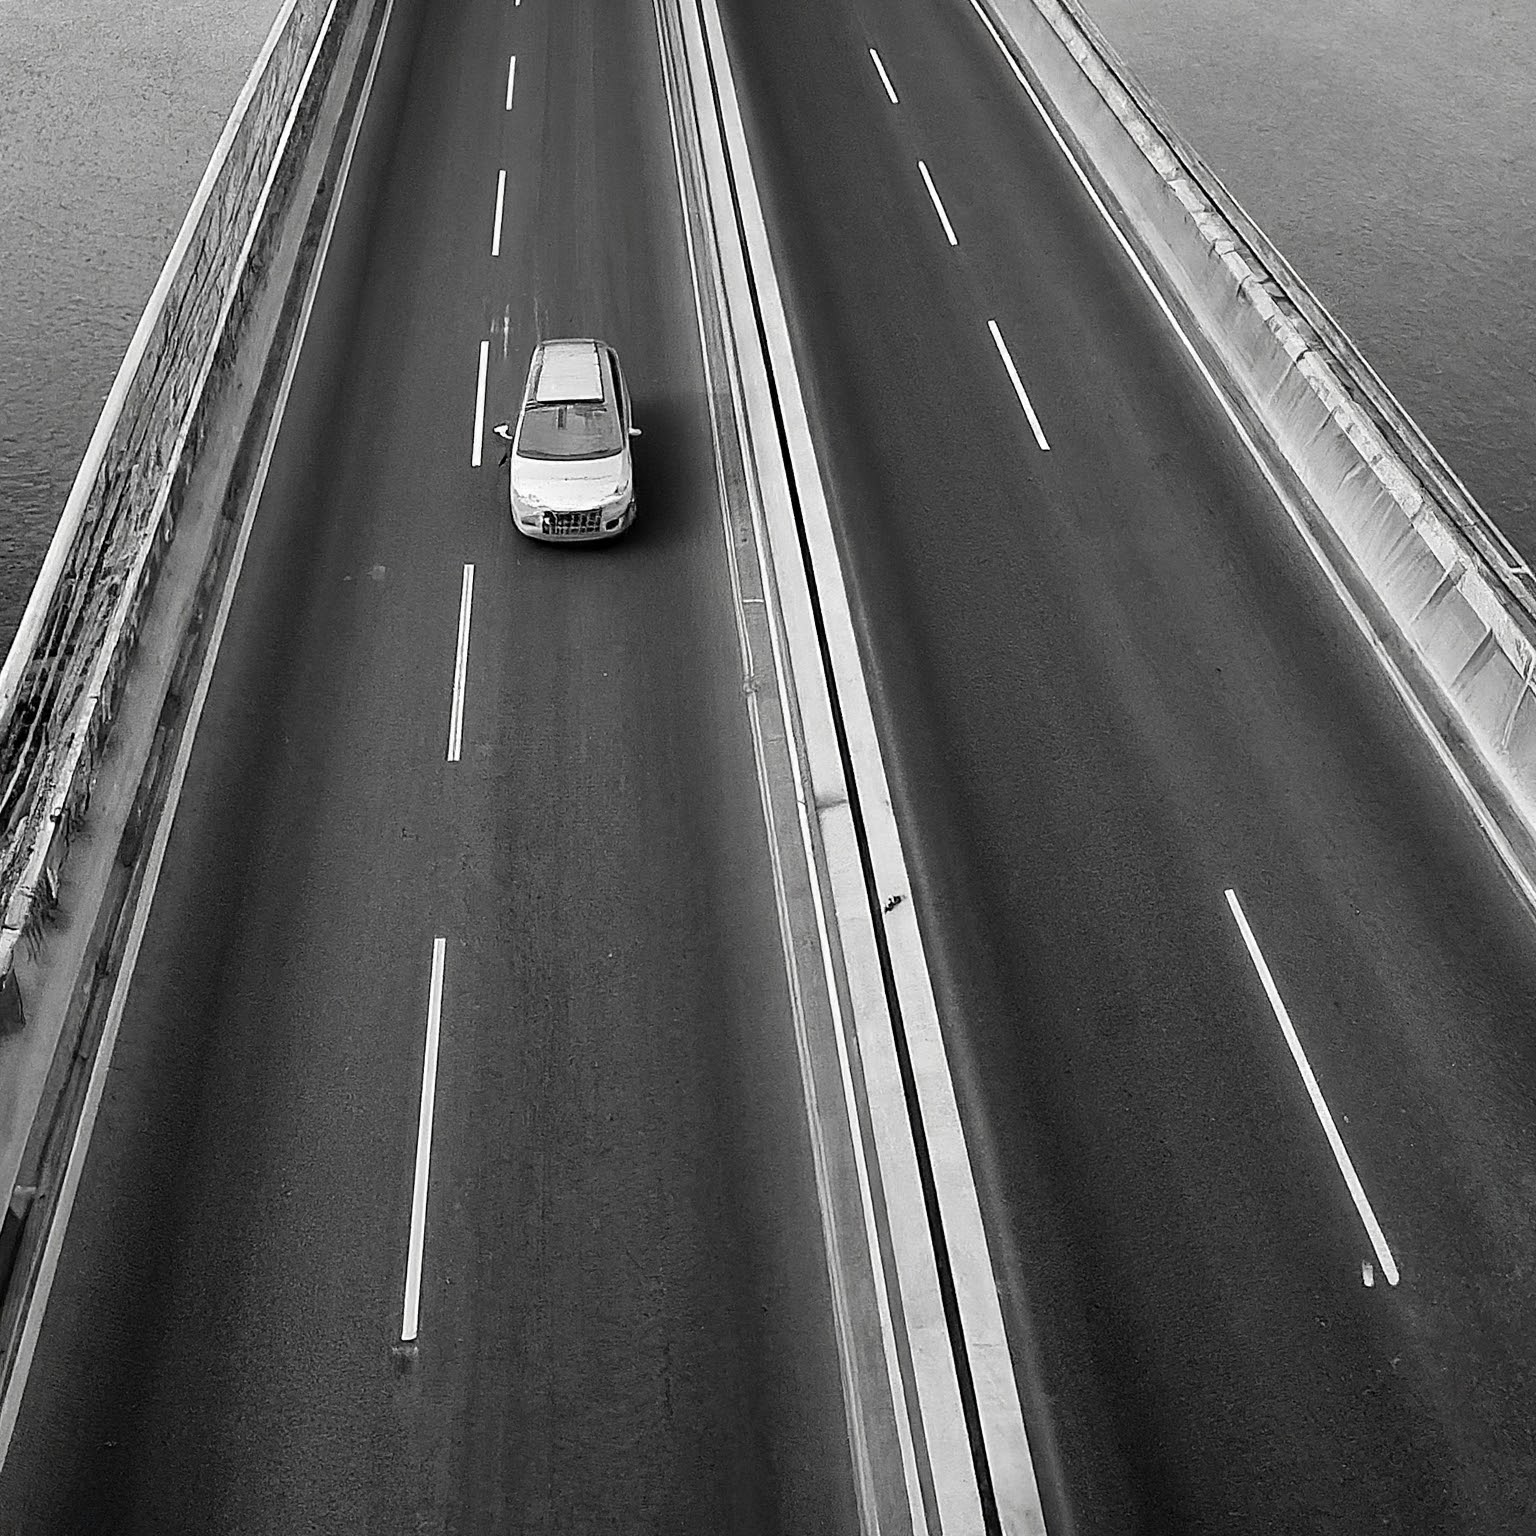
\includegraphics[width=0.3\textwidth]{textual/Figuras/image_fx_driving_a_car_across_a_bridge_black_and_white.jpg}
  \caption{Driving \emph{across} a bridge (Generated using ImageFX by Google).}
  \label{fig: across}
\end{figure}

From the primary idea of ``from one side to the other'', ACROSS can be broken down into four meanings:

%M: Só agora entendi que muitos erros de compilação estão acontecendo porque os exemplos do Linguex estão dentro de ambientes estruturados (itemize, enumerate etc.). Vai ser preciso tirar os exemplos de dentro desss ambientes. O exemplo é um ambiente em si mesmo.

\begin{description}
    \item [Movement over a Surface:] Similar to driving across the bridge, you can move across another surface such as a body of water (e.g.: a river, a lake) (Example~\ref{ex:10}).
\end{description}

    \ex. He sailed \emph{across} the lake.
    \label{ex:10}
    
\begin{description}
    \item [Perpendicular Position:] As described by~\textcite{bruckfield2011prepositions}, the bridge itself can also be described as located (static) across the river, such as in Example~\ref{ex:11}.
\end{description}

    \ex. The bridge \emph{across} the River Kwai has twelve arches. \label{ex:11}
    
\begin{description} 
    \item [Opposite Location:] The preposition ACROSS can also mean ``on the opposite side of'' something \parencite{cambridge-across}, like in Example~\ref{ex:12}.
\end{description}

    \ex. The library is just \emph{across} the road. 
    \label{ex:12}

\begin{description}
    \item [Distribution:] ACROSS can indicate something distributed throughout an area or something that spreads, occupies part of an area, or crosses some kind of surface \parencite{bruckfield2011prepositions}. See Examples~\ref{ex:13} and \ref{ex:14}.
\end{description}

    \ex. Voters \emph{across} the nation will elect a new president. \label{ex:13}

    \ex. The president was wearing the presidential sash \emph{across} his chest. \label{ex:14}


In the figurative sense, ACROSS can represent connections and how something permeates a wider area. For example, a smile spread \emph{across} a person's face can emphasize a broad and genuine sign of happiness. Similarly, in cloud computing, when you update files \emph{across} all your devices, the preposition highlights the interconnectedness between the network. The same way, in the business world, effective communication \emph{across} cultures is crucial for building strong international relationships; that is, \emph{across} underscores the need to bridge cultural gaps and establish connections among different groups.


\subsubsection{The Preposition THROUGH}

According to~\textcite{bruckfield2011prepositions}, THROUGH shares some similarities with ACROSS but extends to movement within a volume rather than over a surface. While ACROSS typically applies to two-dimensional spaces, the core meaning of THROUGH involves movement entering and exiting a three-dimensional space, such as:

\begin{description}
    \item[A Passage:] THROUGH is used to convey movement or direction from one side to the other within a passage or some kind of conduit (e.g., tunnels, channels, etc.), as illustrated in Example~\ref{ex:15}.
\end{description}

    \ex. He drove \emph{through} the tunnel. \label{ex:15}

    \begin{figure}[ht]
    \centering
    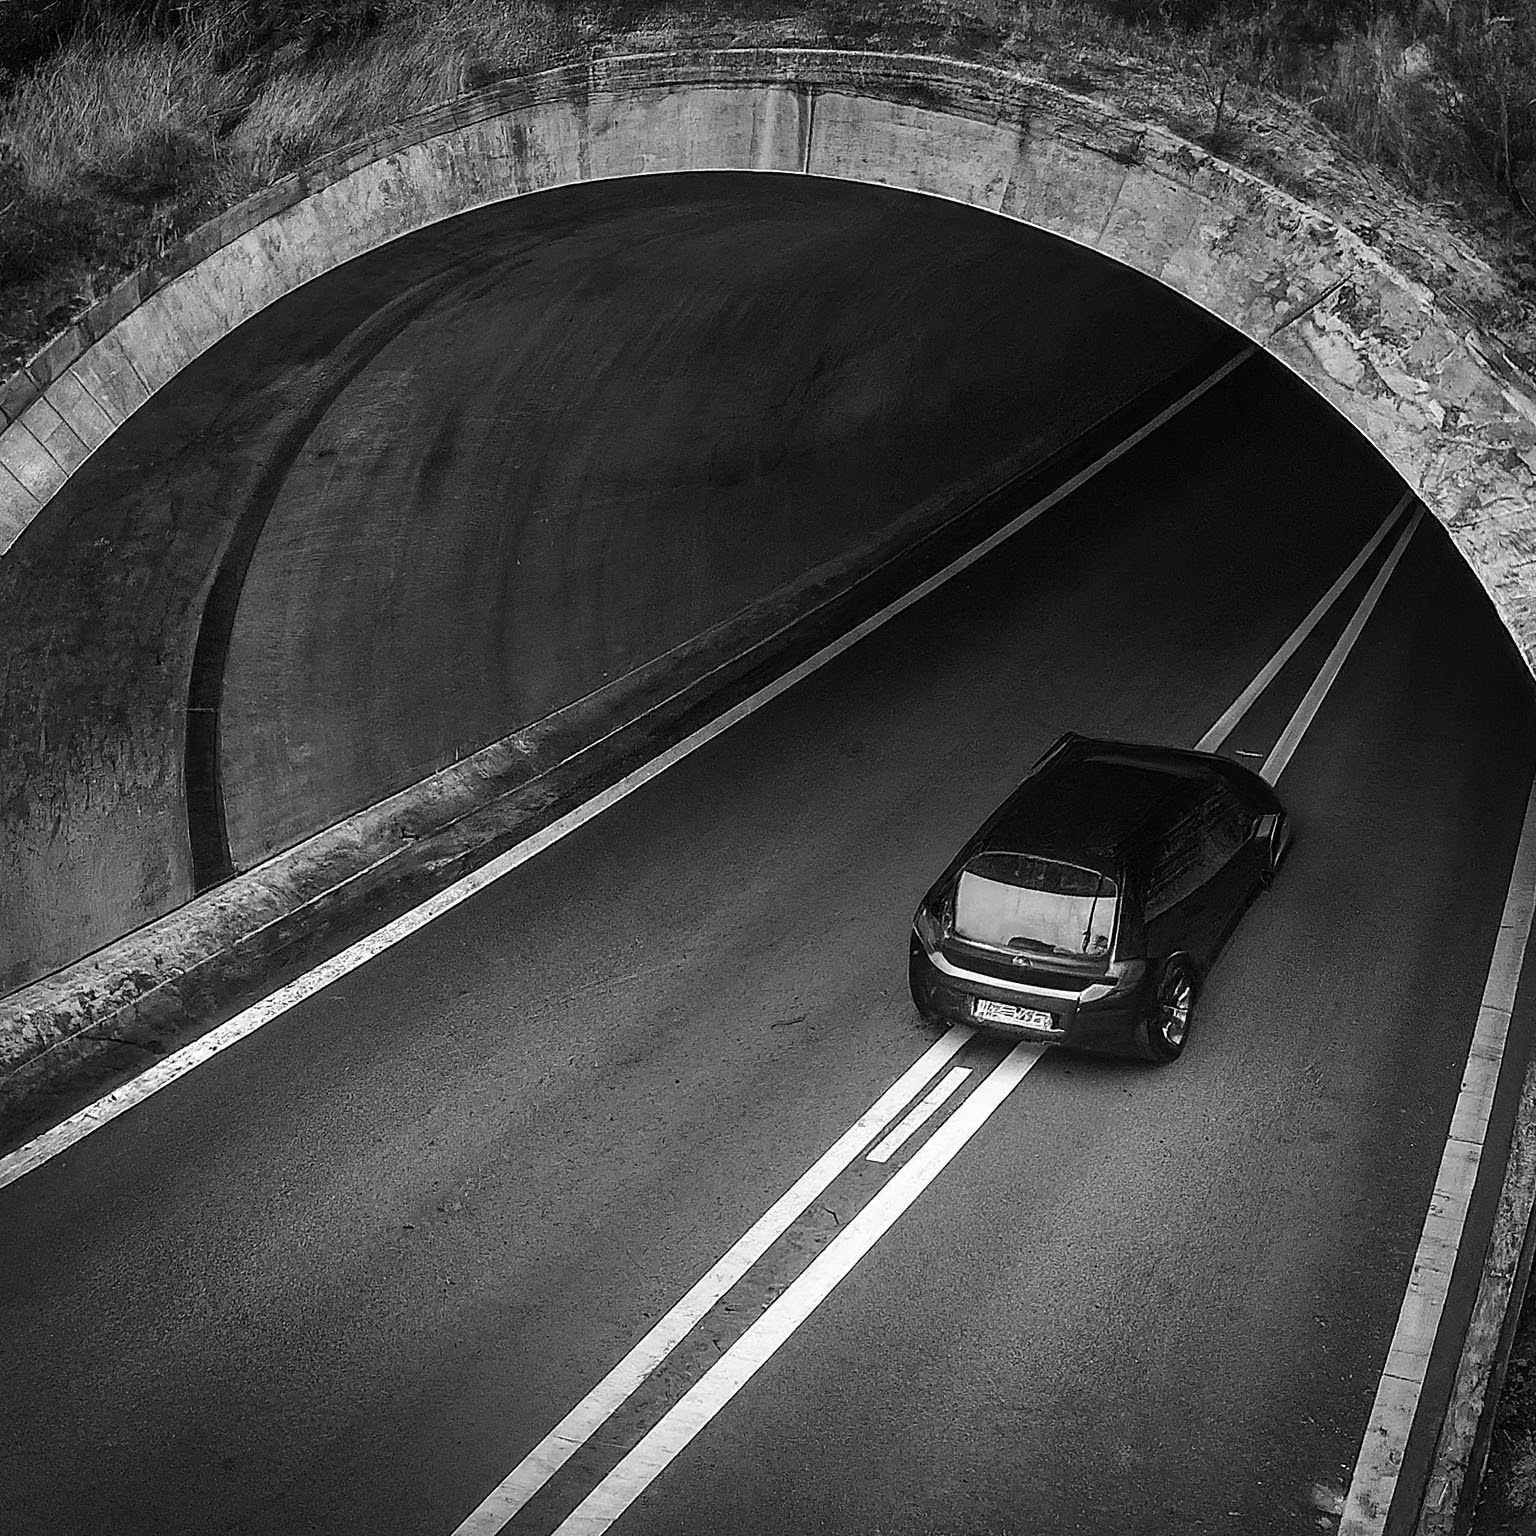
\includegraphics[width=0.3\textwidth]{textual/Figuras/image_fx_a_car_entering__a_tunnel_black_and_white_seen.jpg}
    \caption{Driving \emph{through} a tunnel (Generated using ImageFX by Google).}
    \label{fig:trough-ex-15}
    \end{figure}
    
\begin{description}
    \item[An Open Area:] THROUGH is also used to express movement from one side to the other within an open area, region, or place \parencite{cambridge-through}. See Example~\ref{ex:16}.
\end{description}

    \ex. To reach the museum, I had to walk \emph{through} the park. \label{ex:16}

\begin{description}
    \item[A Barrier:] THROUGH can signify movement past or penetrating a barrier or an obstacle, as illustrated in Examples~\ref{ex:17} and \ref{ex:18}.
\end{description}
    
    \ex. The car drove straight \emph{through} the gate. \label{ex:17}

    \ex. The man hammered a nail \emph{through} the board. (see Figure~\ref{fig:through}) \label{ex:18}
    
    \begin{figure}[ht]
    \centering
    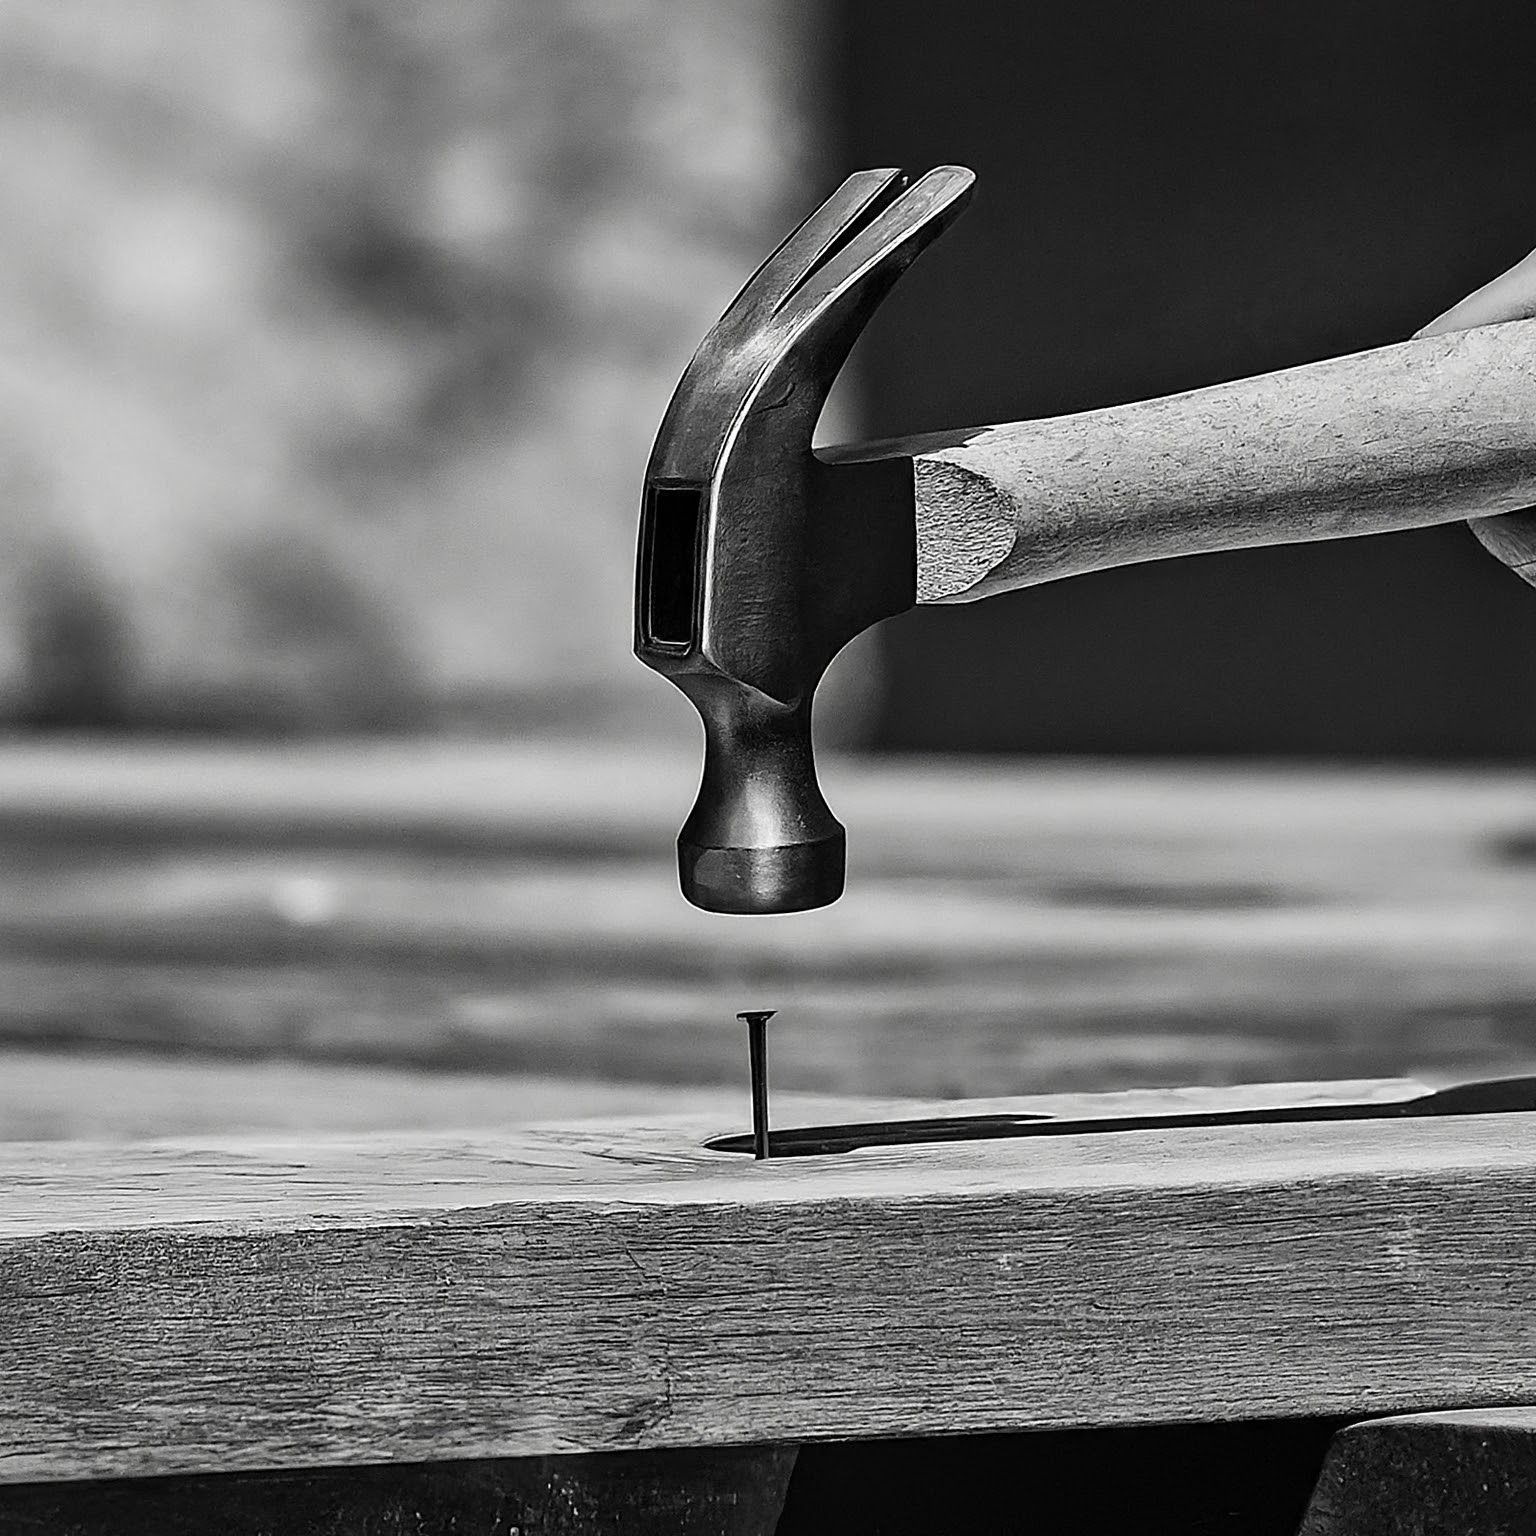
\includegraphics[width=0.3\textwidth]{textual/Figuras/image_fx_hammering_a_nail_through_a_wooden_board_black.jpg}
    \caption{Hammering a nail \emph{through} a wood board (Generated using ImageFX by Google).} \label{fig:through}
    \end{figure}
    
\begin{description}
    \item[Part of a Route:] THROUGH can also indicate a static location or movement along a route or path, as in Example~\ref{ex:19}.
\end{description}
     
    \ex. The sauna is \emph{through} the bathroom. \label{ex:19}


Beyond literal movement, the preposition THROUGH can be used figuratively. For instance, it can mean experiencing something indirectly, such as with a tool or medium (e.g., ``He was looking at the moon \emph{through} the binoculars''), describing a particular method (e.g., ``I like to build relationships \emph{through} trust and understanding'') or seeing from a perspective (e.g., ``I never saw their story \emph{through} their eyes'').


\subsubsection{The Preposition INTO}

The preposition INTO indicates ``movement in the direction of a container and the entry in the container'' \parencite{bruckfield2011prepositions}. It can be expanded into two specific meanings:

\begin{description}
    \item[Entering an Enclosure:] INTO is typically used for movement or direction ``to the inside or middle of a place, container, area, etc.'' (Example~\ref{ex:20}) \parencite{cambridge-into}.
\end{description}
    
    \ex. The boy kicked the ball \emph{into} the box. (see Figure~\ref{fig: into}) \label{ex:20}

    \begin{figure}[ht]
    \centering
    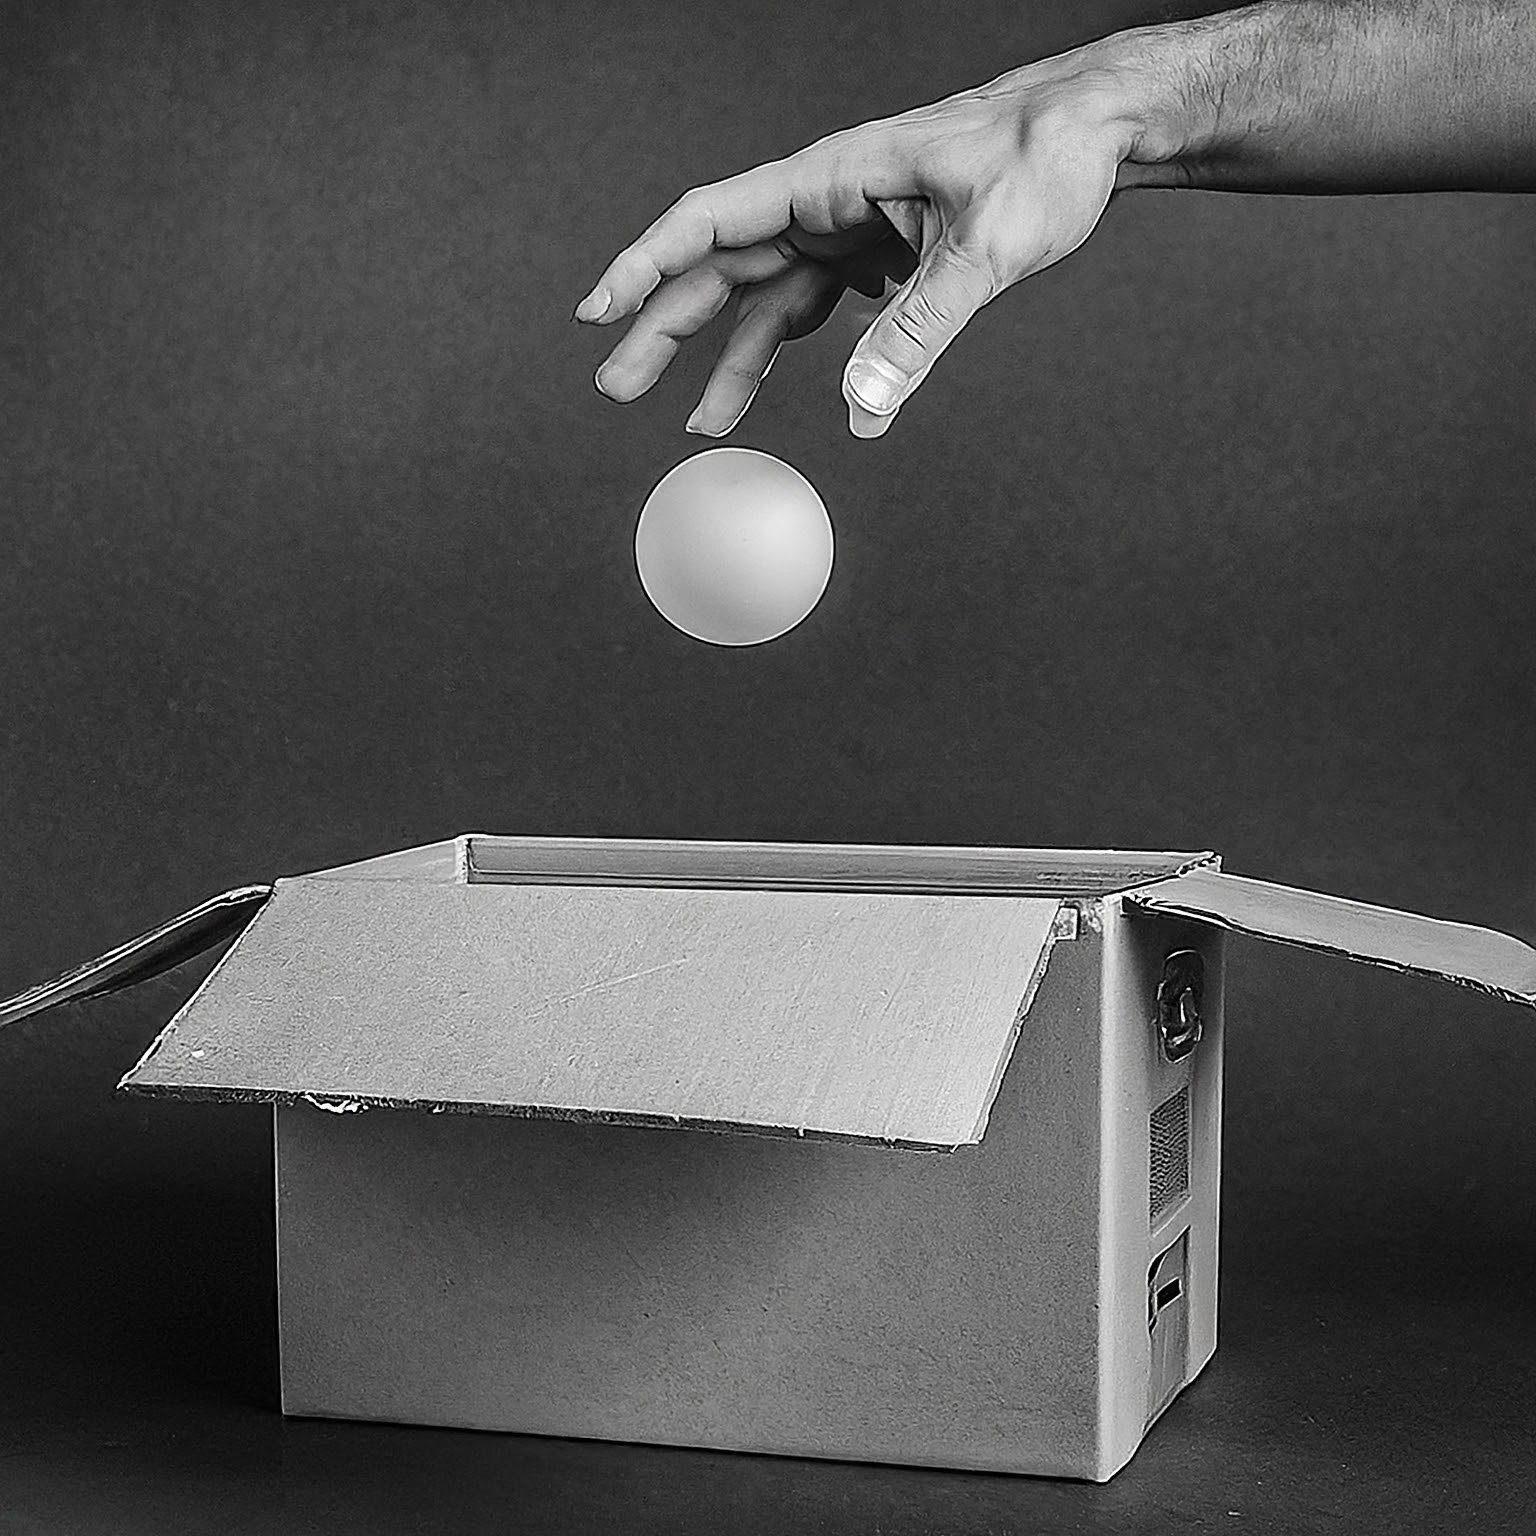
\includegraphics[width=0.3\textwidth]{textual/Figuras/image_fx_hand_throwing_a_ball_into_an_open_cardboard_b.jpg}
    \caption{The ball is going \emph{into} the box (Generated using ImageFX by Google).}
    \label{fig: into}
    \end{figure}
    
\begin{description}   
    \item [Movement with Force:] INTO indicates movement with force that usually results in collision with something else, but without moving inside of it, as in  Examples~\ref{ex:21} and \ref{ex:22}.
\end{description}
    
    \ex. The car crashed \emph{into} the wall. \label{ex:21}
    
    \ex. I wasn't looking where I was going and walked \emph{into} a lamppost. \label{ex:22}         


Beyond literal movement, INTO figuratively implies entering a new state (e.g.: ``She went \emph{into} a depression''), condition (e.g.: ``He went \emph{into} surgery''), transformation (e.g.: ``This software transforms your computer \emph{into} a piano''), etc. 


\subsubsection{The Preposition ONTO}
ONTO implies movement towards a surface, crossing a boundary into or onto the surface, regardless of its shape or position, as described by~\textcite{bruckfield2011prepositions} (see Figure~\ref{fig: onto}). 

    \begin{figure}[ht]
    \centering
    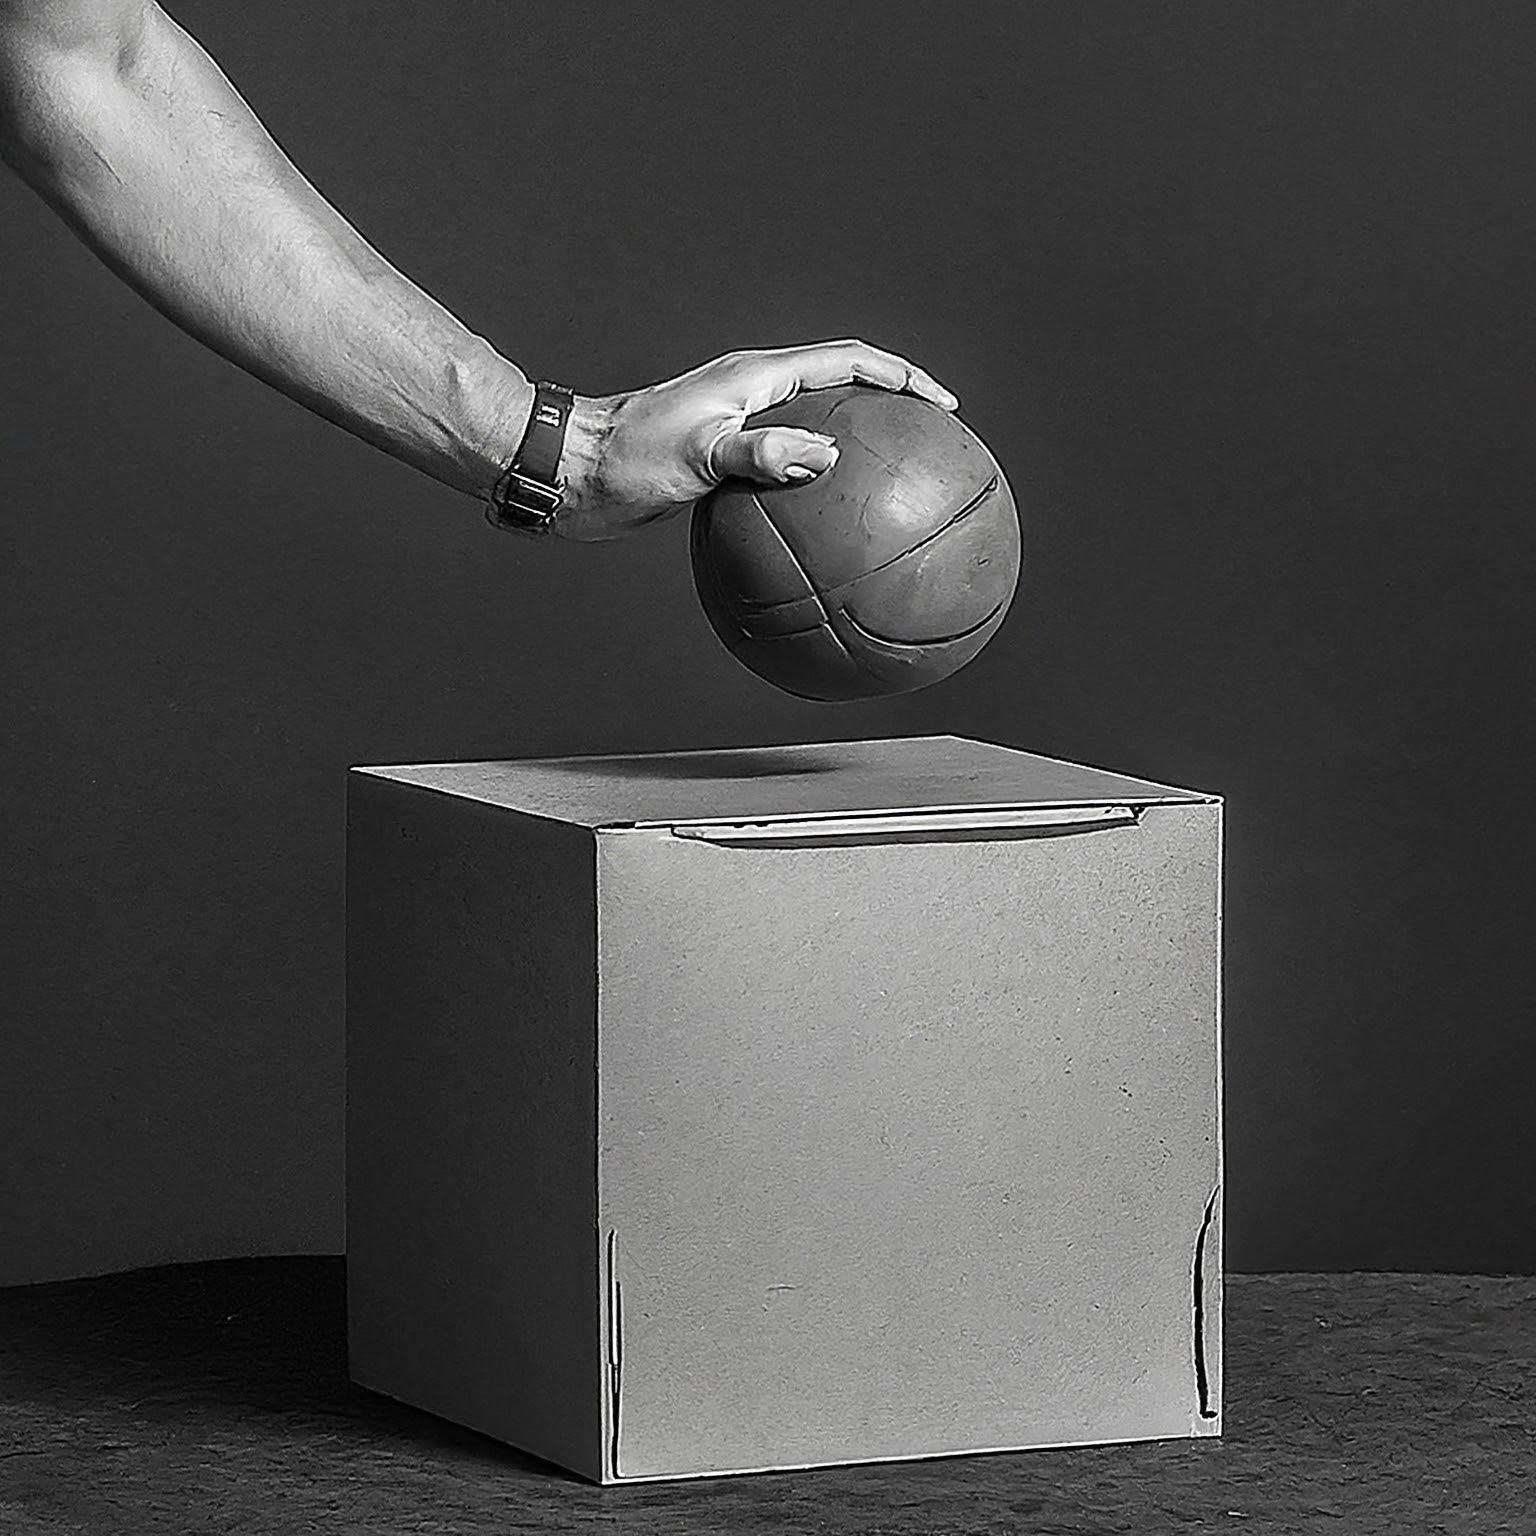
\includegraphics[width=0.3\textwidth]{textual/Figuras/image_fx_placing_a_ball_onto_a_closed_cardborad_box_bl.jpg}
    \caption{The ball is going \emph{onto} the box (Generated using ImageFX by Google).}
    \label{fig: onto}
    \end{figure}

\begin{description}
    \item[Movement towards a surface:] movement from an initial position to a final one on a surface (Example~\ref{ex:23}).
    
\end{description}
    
    \ex. I tossed the keys \emph{onto} the desk. \label{ex:23}
    
\begin{description}    
    \item [Sense of Attachment:] can imply a sense of attachment or pressure (Example~\ref{ex:24}).
\end{description}    
    
    \ex. He strapped the backpack \emph{onto} his shoulders and started hiking. \label{ex:24}
    

While both ONTO and ON relate to surfaces, \textcite{bruckfield2011prepositions} explains they differ based on movement versus final location. We use ONTO for movement towards a surface, whereas ON indicates something already resting on a surface. See Examples~\ref{ex: 25} and \ref{ex: 26}.

\ex. The father lifted the child \emph{onto} his shoulders. \label{ex: 25}

\ex. The father lifted the child \emph{on} his shoulders. \label{ex: 26}

In Example~\ref{ex: 25}, the child was initially in a lower position (e.g.: on the floor or on the baby pram) and was sat on the father's shoulders. In Example~\ref{ex: 26}, however, the father's shoulders was the initial support from which the child was lifted to a higher position.

Figuratively, ONTO goes beyond physical movement. For instance, it can suggest encountering something unexpectedly (``stumbling \emph{onto} a problem''), the final stages of a process (``putting the finishing touches \emph{onto} a plan''), awareness (``only one news channel was \emph{onto} the case''), or  attention (``the boss was \emph{onto} me) \parencite{cambridge-onto}. 


\subsection{Challenges in Translating Spatial Prepositions}
\label{subsec: Challenges in Spatial Prepositions}

This section explores the complexities of translating spatial prepositions between English (EN) and Brazilian Portuguese (PT-br), building upon the analysis of prepositional semantics. Particularly, it examines how PT-br often employs different prepositions, prepositional phrases, or parts of speech compared to EN to convey similar meanings.

\subsubsection{ACROSS \& THROUGH vs.\ `Através de': Similarities and Divergences}

In an preliminary study, \textcite{McCleary-Viotti-2004} provides valuable insights into the challenges of translating EN spatial prepositions like ACROSS and THROUGH using the PT prepositional phrase ``através de''. Their work draws on~\textcite{talmy2000towardb}'s proposition that languages select spatial elements from a finite universal inventory and combine them into ``schemas'' typically expressed by closed-class forms (such as prepositions). However, they argue that PT-br might rely more heavily on open-class forms (verbs and nouns) for spatial representation compared to EN. For instance, they present Example~\ref{ex:32}.

\ex. There is a barrier \emph{across} the road. (See Figure~\ref{fig:barrier}) \label{ex:32} \\
     ? Tem uma barreira \emph{através d}a estrada. \\
     Tem uma barreira (\emph{atravessada}) \emph{n}a estrada.

\begin{figure}[ht]
    \centering
    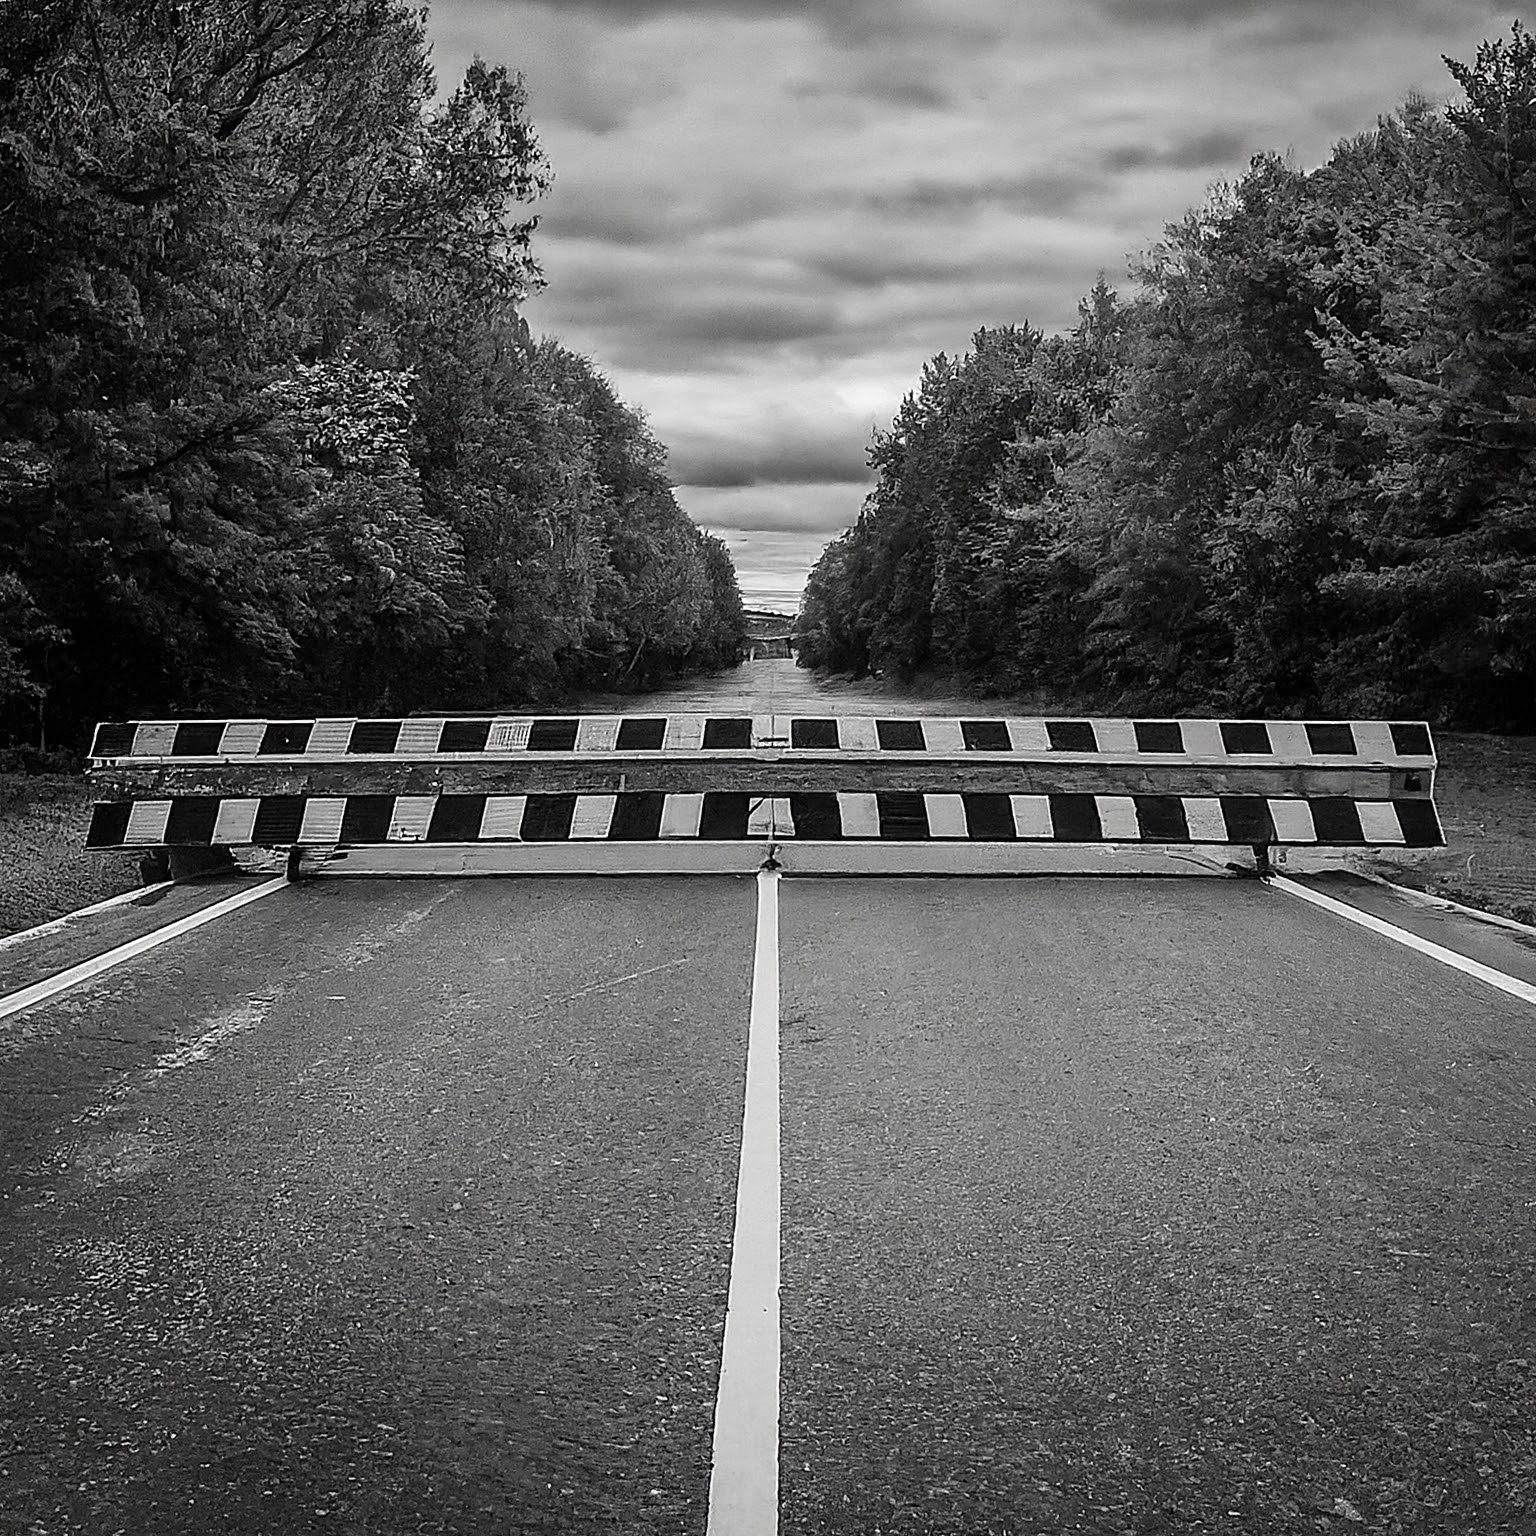
\includegraphics[width=0.3\textwidth]{textual/Figuras/image_fx_a_barrier_across_the_road_black_and_white.jpg}
    \caption{A barrier \emph{across} the road (Generated using ImageFX by Google).}
    \label{fig:barrier}
\end{figure}
    
As discussed by~\textcite{McCleary-Viotti-2004}, while ``através de'' might seem like a direct translation of ACROSS, it aligns more closely with the schema of the preposition THROUGH, which, as discussed in Section~ \ref{sec: Spatial Prepositions}, represents movement in and out of a three-dimentional space, such as a volume. Nevertheless, in Example~\ref{ex:32}, ACROSS depicts ``the barrier'' as positioned parallel to ``the road'' (a two-dimensional space). To convey this concept, PT-br necessitates a verbal phrase, such as the past participle form ``atravessada'' (crossed), to emphasize the barrier's location in relation to the road's limits, highlighting the preference for open-class forms. To illustrate the similarity between ``através de'' and THROUGH, \textcite{McCleary-Viotti-2004} use Examples \ref{ex:33} and \ref{ex:34}. Note that, in this case, another prepositional phrase (por + a/o -- pelo, pela) is also possible.

\ex. Eles abriram um túnel \emph{através d}a/\emph{pel}a montanha. \label{ex:33}   \\
     They dug a tunnel \emph{through} the mountain.
      
\ex. A luz entrava \emph{através d}as/\emph{pel}as janelas do mosaico. (See Figure~\ref{fig:window})  \label{ex:34}  \\  
    The light entered \emph{through} the stained-glass windows. 

\begin{figure}[ht]
    \centering
    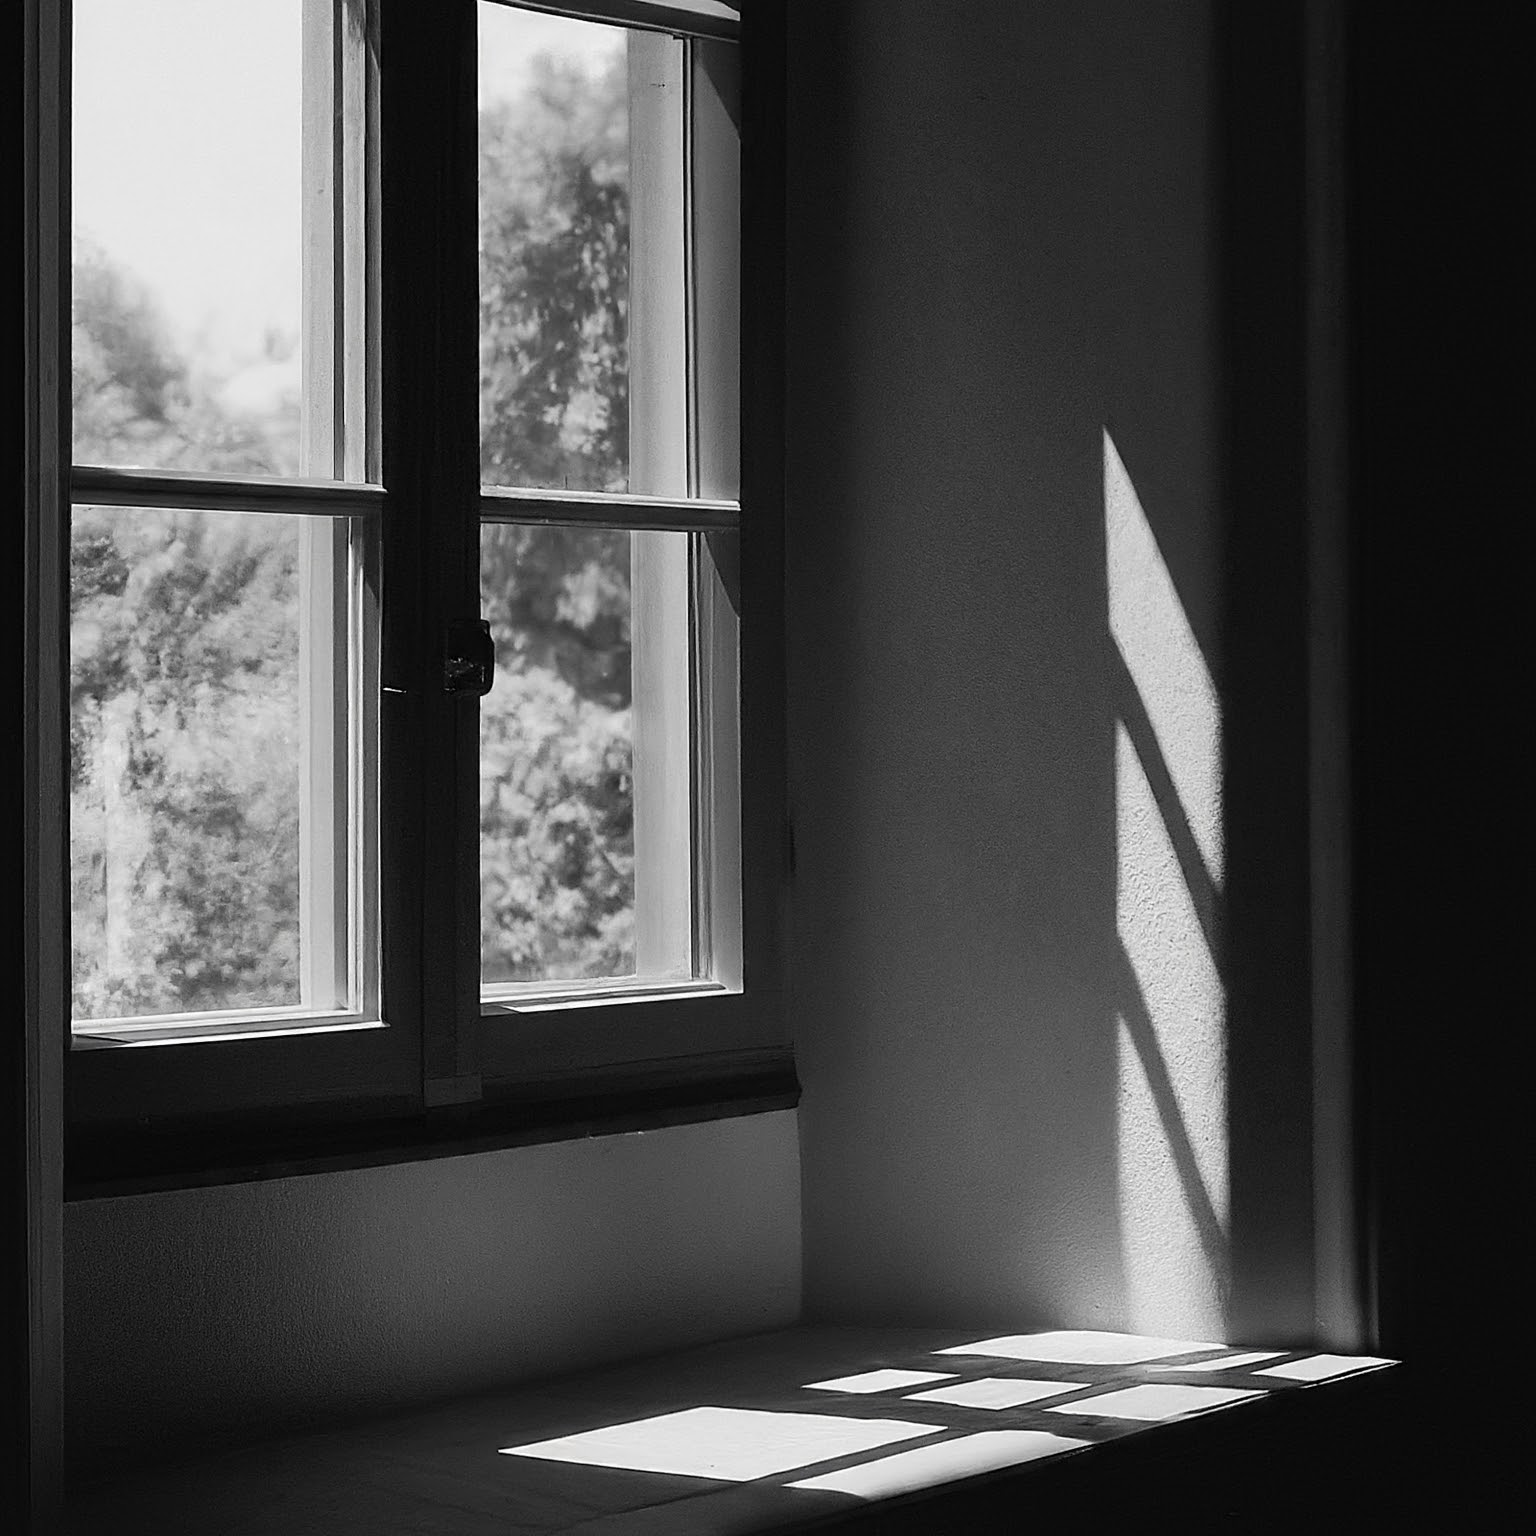
\includegraphics[width=0.3\textwidth]{textual/Figuras/image_fx_light_shining_through_a_window_black_and_whit.jpg}
    \caption{Light shining \emph{through} a window (Generated using ImageFX by Google).}
    \label{fig:window}
\end{figure}


Examples~\ref{ex:33} and \ref{ex:34} illustrate motion within 3-D spaces (e.g.,``the montain'' and ``the window''), highlighting the parallels between the EN and PT-br prepositions in these contexts. However, this similarity should be approached with caution. As~\textcite{McCleary-Viotti-2004} point out, THROUGH and ``através de'' are not always interchangeable, as ``através de'' typically emphasizes the process of movement or action, rather than the final outcome. This distinction explains why the prepositional phrase in Examples~\ref{ex:35} and \ref{ex:36} is unacceptable in PT-br.

\ex. He hammered a nail \emph{through} the board. \label{ex:35}   \\
     ? Ele bateu/martelou um prego \emph{através d}a tábua. \\
     Ele bateu/martelou um prego \emph{que atravessou a}/\emph{n}a tábua.

\ex. Frankenstein's monster has a bolt \emph{through} his neck. \label{ex:36}   \\
     ? O monstro de Frankenstein tem um pino \emph{através d}o pescoço. \\
     O monstro de Frankenstein tem um pino (\emph{atravessado}) \emph{n}o pescoço.

In both Examples \ref{ex:35} and \ref{ex:36}, the scopes of ``através'' are final states (results) --- the nail gone through the board and the pin positioned in the creature's neck, respectively. This differs from ``através da montanha'' and ``através da janela,'' in that ``através'' emphasizes the process --- workers opening the tunnel and light entering the room. This distinction between describing a process (activity) versus a final state (result) is crucial for using the preposition effectively. In summary, as explained by~\textcite{McCleary-Viotti-2004}, ``através'' is only suitable when the phrase it precedes entails a process-type event structure (activity) or one that has as a sub-event a transition (achievement) or a process (accomplishment).


\subsubsection{The Versatility of PT-br Preposition `em'}

A descriptive study by~\textcite{oliveira2012cognitive} investigates the multiple meanings of the PT-br preposition ``em'' based on Langacker's Schematic Network model \parencite{langacker1987foundations}. The analysis of a massive dataset of journalistic texts (1.2 million words) published between 2007 and 2008 revealed that while ``em'' often conveys location, it can also take on other meanings unlike similar prepositions in other languages (e.g., French \emph{dans,} English \emph{in}). 
This versatility is further emphasized by the fact that it frequently appears blended with articles, numerals, and demonstrative pronouns through the root ``n-''. Due to its broader range of usage, ``em'' is highly dependent on the surrounding text for its specific meaning.

One way to understand the complexities of ``em'' is by examining the schemas associated with it. The two most  prototypical meanings, as explained by~\textcite{oliveira2012cognitive}, are the CONTAINER (see Figure~\ref{fig: container}) and CONTACT (see Figure~\ref{fig: contact}). The CONTAINER schema captures the notions of `inclusion' and `closure,' as illustrated in Example~\ref{ex:container}. The CONTACT schema, on the other hand, focuses on the concept of `support,' where ``em'' describes the relationship between the Figure and a surface it interacts with (Ground) (see Example~\ref{ex:contact}).

\ex. Imaginem o suco \emph{num} copo. \newline \label{ex:container}
[Imagine the juice \emph{in} a glass.]

\begin{figure}[ht]
\centering
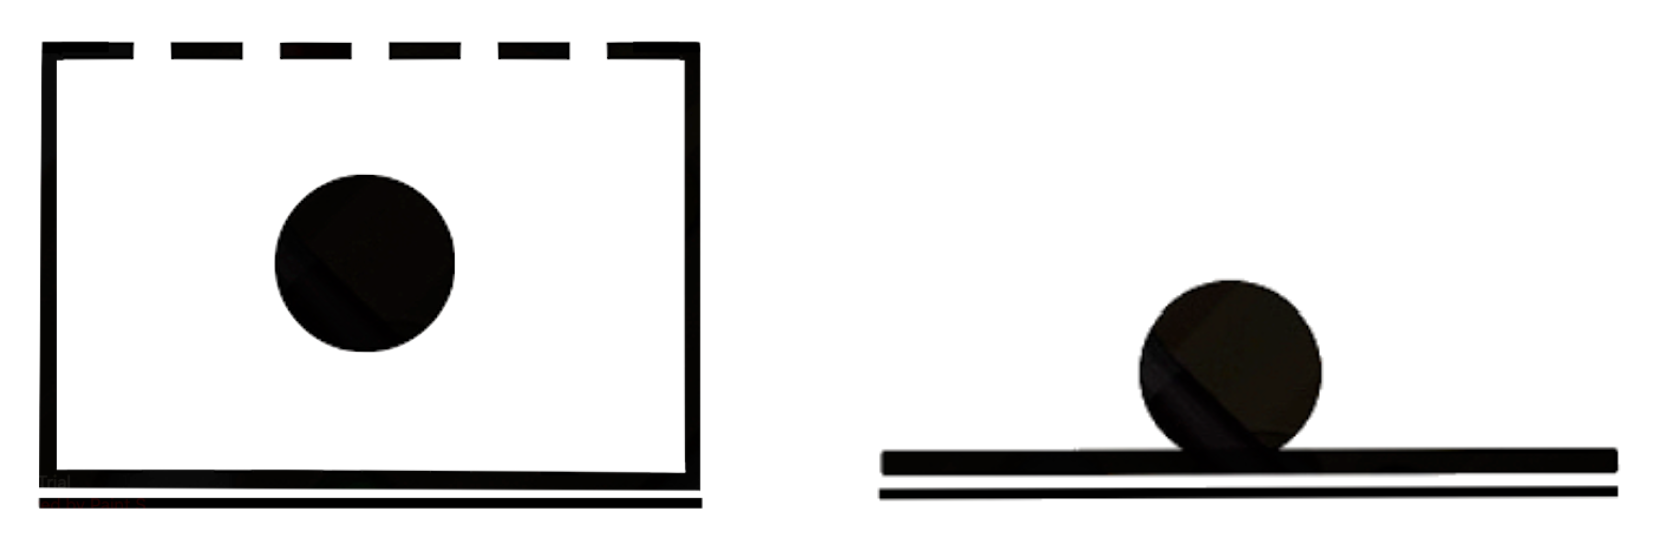
\includegraphics[width=0.6\textwidth]{textual/Figuras/Untitled design.png}
\caption{The CONTAINER vs. CONTACT schemas.}
\label{fig: container}
\end{figure}

\ex. Se for preciso, vamos acampar \emph{na} quadra. (E. de Minas -- Aug.05.2008) \newline [If necessary, we shall camp \emph{on} the court.] \label{ex:contact}

\begin{figure}[ht]
\centering
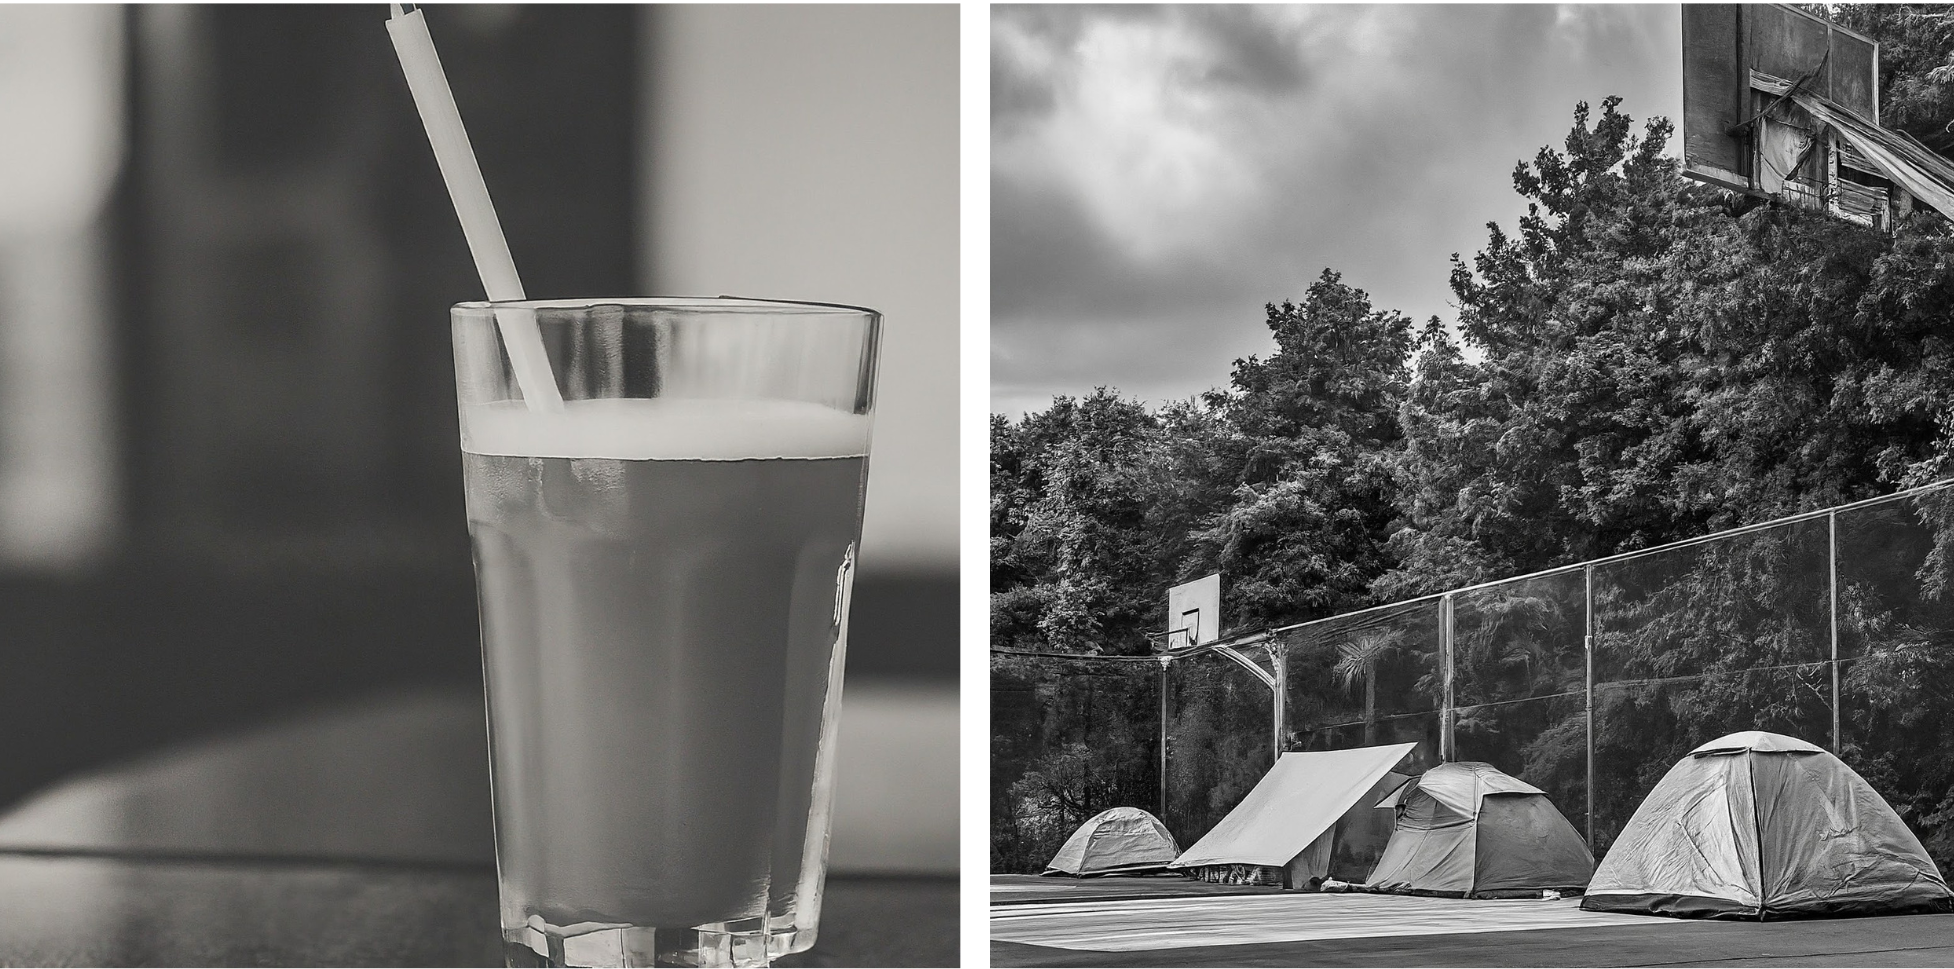
\includegraphics[width=0.6\textwidth]{textual/Figuras/Untitled design-2.png}
\caption{Conceptualizations: ``\emph{num} copo'' vs. ``\emph{na} quadra'' (Generated using ImageFX by Google).}
\label{fig: contact}
\end{figure}


However, the concept of movement with ``em'' presents an interesting nuance within the schema framework. Although typically signifying location rather than movement, as \textcite{oliveira2012cognitive} suggests, in dynamic contexts, ``em'' can locate an object at the endpoint of a Path, implying a ``caused motion'' schema. As illustrated in sentences \ref{ex:em-into} and \ref{ex:em-at} from \textcite{oliveira2012cognitive},  where ``em'' highlights the final location of the sewage and thrown objects, irrespective of the surface being a pond, field, or something else entirely. This suggests that schemas associated with ``em'' might be more flexible than initially conceived,  potentially incorporating a ``caused motion'' aspect in specific contexts where movement is implied by the situation (e.g., throwing, dumping).

\ex. Depoimentos de moradores, fotografias, vídeos e a análise da água mostram que esgoto sem tratamento está sendo despejado \emph{na} lagoa. (Estado de Minas – Aug.06.2008) \label{ex:em-into} \newline
[Residents’ reports, photos, videos, and the analysis of the water show that untreated sewage has been dumped \emph{into} the pond.]

\ex. Além de uma faixa com os dizeres “Queremos um time de verdade”, bonecas, pipocas e bananas foram jogadas \emph{no} gramado. (Estadão -- Jun.24.2008) \label{ex:em-at} \newline
[Besides a banner which read “We want a real team”, puppets, popcorn and bananas were thrown \emph{onto} the field.]


In addition, \textcite{Ferreira-Basso-2020} clarify that the directional or goal-related interpretation of ``em'' is a false syncretism arising from the presence of verbs indicating movement in the structure. In sentences like Example~\ref{ex:em-goal}, ``em'' emphasizes that the Figure (the entity) ends up \emph{inside} the Goal after the movement, establishing a static locative relationship at the event's conclusion. However, in structures without such verbs, like in Example~\ref{ex:em-loc}, ``em'' is interpreted as merely locative, describing the Figure's static position relative to the Ground (the reference point), thereby reinforcing its understanding as a locative preposition.

\ex. Pedro correu \emph{na} farmácia.\label{ex:em-goal} \newline
[Peter ran \emph{to} the pharmacy.]

\ex. Ana almoçou \emph{no} shopping.\label{ex:em-loc} \newline
[Ana had lunch \emph{at} the shopping mall.]


\textcite{oliveira2012cognitive} also explores situations where the Figure lacks a physical presence. In these cases, the Ground, also referred to as the ``Medium'', can involve the absence of something within it, like a ``hole'' in a wall. These missing parts are called ``empty spatial trajectors.'' According to~\textcite{oliveira2012cognitive}, the viewer mentally completes the missing part of the surface, creating a space for the ``hole''. In this configuration, the boundary of the Ground and the external boundary of the Figure overlap. Example~\ref{ex: em-into-through} illustrates this case where ``em'' could be translated as either INTO or THROUGH in EN, depending on more specific details of the Path taken by the drill. In PT-br, if we want to emphasize the crossing aspect, we can use ``atravessado'' for THROUGH. Figure~\ref{fig: hole-wall} demonstrates the concept in PT-br, where the broken line depicts the completed wall and the shaded region represents the hole. Additionally, Figure~\ref{fig:hole-wall2} shows the different scenarios for ``em'' as INTO vs. THROUGH.

\ex. O homem furou um buraco \emph{na} parede. \label{ex: em-into-through} \newline
[The man drilled a hole \emph{into}/\emph{through} the wall.] 


\begin{figure}[ht]
\centering

\includegraphics[width=0.2\textwidth]{textual/Figuras/Screen Shot 2024-05-28 at 19.46.20.png}
\caption{Closure of the landmark during conceptualization in PT-br.}
\label{fig: hole-wall} 
\end{figure}

\begin{figure}[ht]
\centering
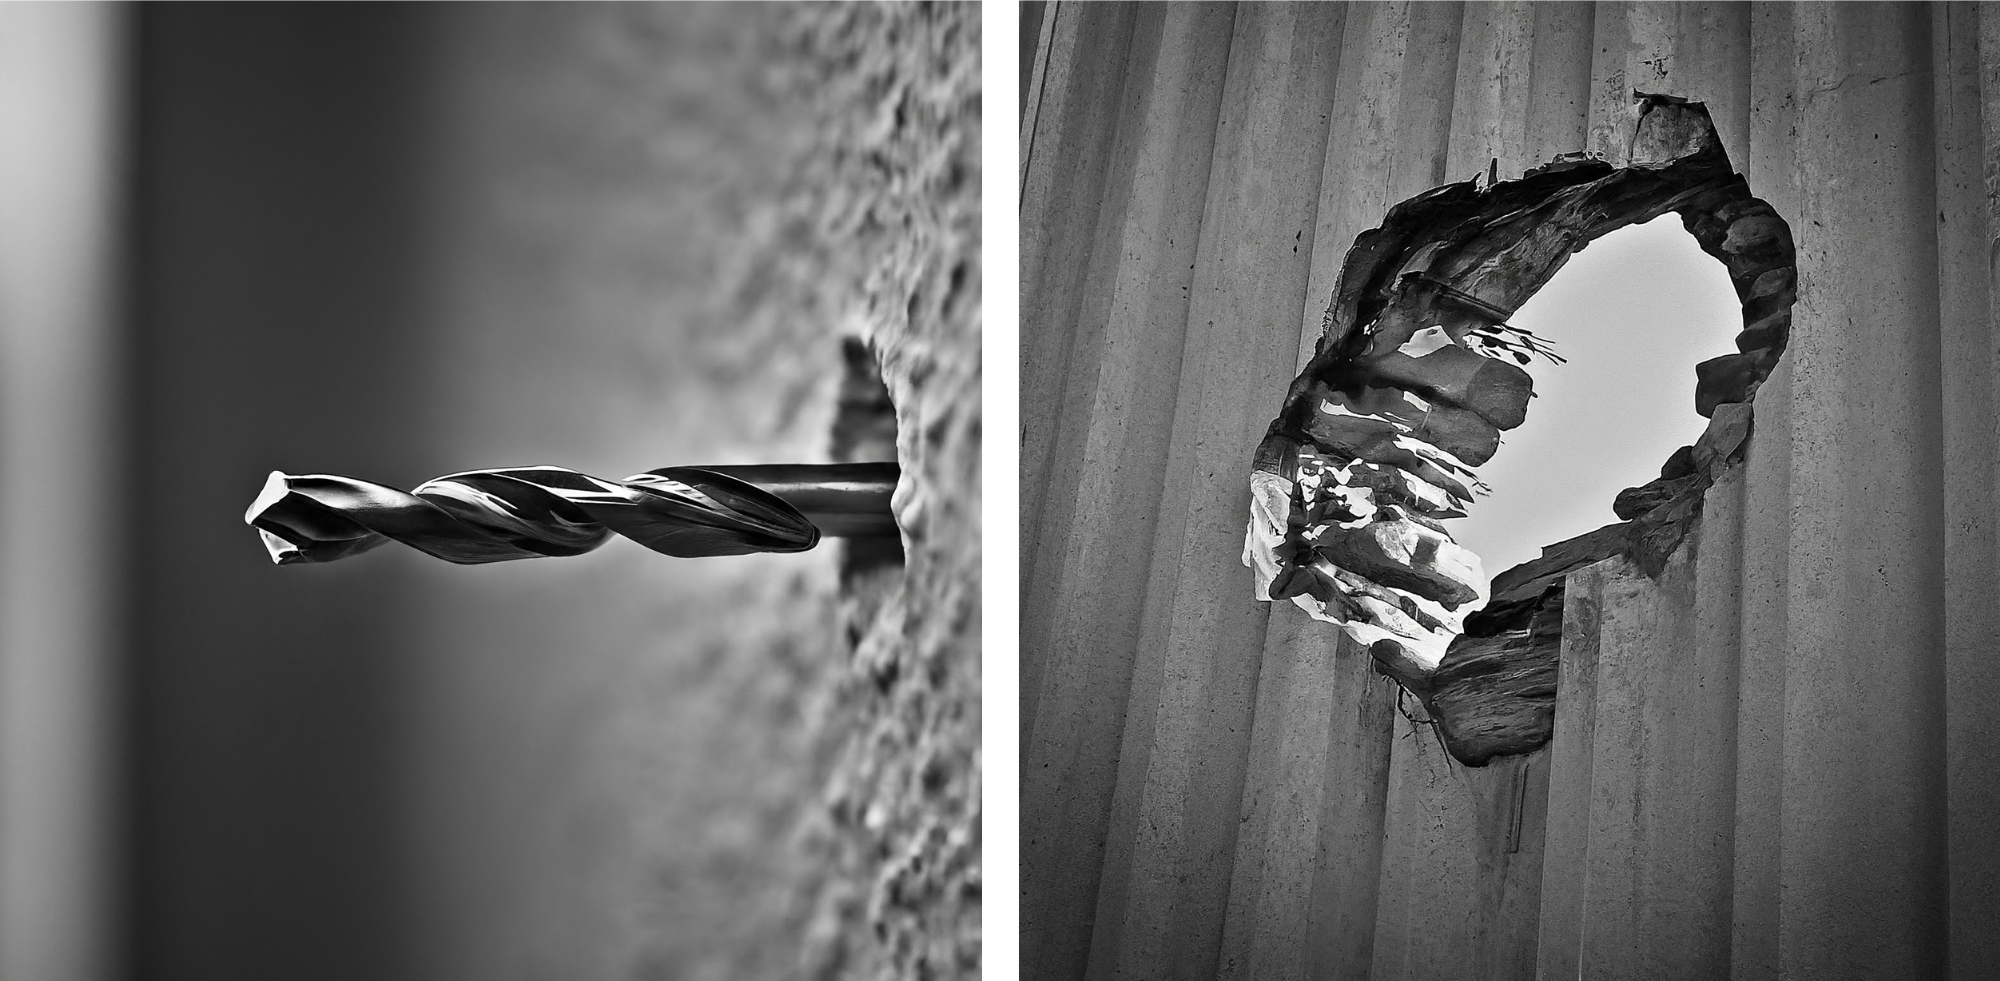
\includegraphics[width=0.6\textwidth]{textual/Figuras/Untitled design-4.png}
\caption{INTO (left) vs. THROUGH (right): ``um buraco  \emph{na} parede'' (Generated using ImageFX by Google).}
\label{fig:hole-wall2} 
\end{figure}

As emphasized by~\textcite{oliveira2012cognitive}, entities like holes, cracks, perforations of any sort must be construed the same way as any concrete object. Besides, the idea of inclusion might not be so emphasized using ``em'' in PT-br as in EN with INTO, for instance. The complex  ``dentro de'' (inside; in) is the one to convey ``inclusion'' in PT-br.

\vspace{0.5em} % Adjust the value (e.g., 1em) to increase or decrease the gap

To sum up, in Section~\ref{sec: translating-spatial}, we detailed the challenges of translating spatial prepositions between EN and PT-br, particularly focusing on issues like polysemy, where a single EN preposition may correspond to multiple meanings, complicating its translation into PT-br. Additionally, the structural differences between the two languages mean that EN often relies on prepositions to convey spatial relationships, while PT-br typically expresses these meanings through verbs. As we transition to the next topic, it is critical to examine these complexities to fully understand the translation difficulties at stake.


\section{Neural Machine Translation}
\label{sec: nmt}

\epigraph{Going to Mars is less relevant than being understood. Language is the tool to solve all the other problems. \\ \hfill --- Marco Trombetti, Co-Founder \& CEO, Translated, Pi Campus}

This section explores the evolution of MT, from early approaches to the state-of-the-art: Neural Machine Translation (NMT). We delve into NMT's architecture, including its encoder-decoder structure and attention mechanism, while also discussing its limitations. We then compare recurrent and transformer-based NMT systems, contrasting their information flow handling. Finally, we discuss the emerging impact of Large Language Models (LLMs) on NMT and the challenges associated with their integration.


\subsection{A Response to Translation Challenges}

The dream of automatic language translation has captivated researchers since the dawn of computing. Early efforts, like those undertaken during World War II code-breaking, laid the groundwork for the field. For many years, Statistical Machine Translation (SMT) and Rule-Based Machine Translation (RBMT) dominated the MT landscape, each offering valuable contributions. However, both approaches encountered limitations \parencite{koehn2020neural}.

Alternatively, according to~\textcite{koehn2020neural}, NMT has emerged as a  significant advancement in recent years in an attempt to overcome the issues presented by previous methods. For instance, as~\textcite{koehn2012statistical} points out, SMT systems often struggled with rare or unseen words, lack of context awareness, and limited ability to capture complex relationships within a sentence. RBMT, on the other hand, faced challenges in creating comprehensive and accurate linguistic rules, handling idiomatic expressions and language nuances, and adapting to new languages or domains \parencite{shiwen2014rule}.

This shift from word-for-word translation to an approach that considers context and provides better resuts on long-range dependencies allows NMT to generate more natural and accurate translations. According to~\textcite{lakew2019multilingual}, state-of-the-art NMT systems achieve this by relying on a key triad: an \emph{encoder} that analyzes the source sentence, a \emph{decoder} that generates the target language translation, and an \emph{attention} mechanism that allows the decoder to focus on relevant parts of the source sentence during translation (see Figure~\ref{fig: Encoder-decoder-attention} for a visual representation). However, these systems differ in how they handle the source sentence, leading to variations in performance.

\begin{figure}[ht]
\centering
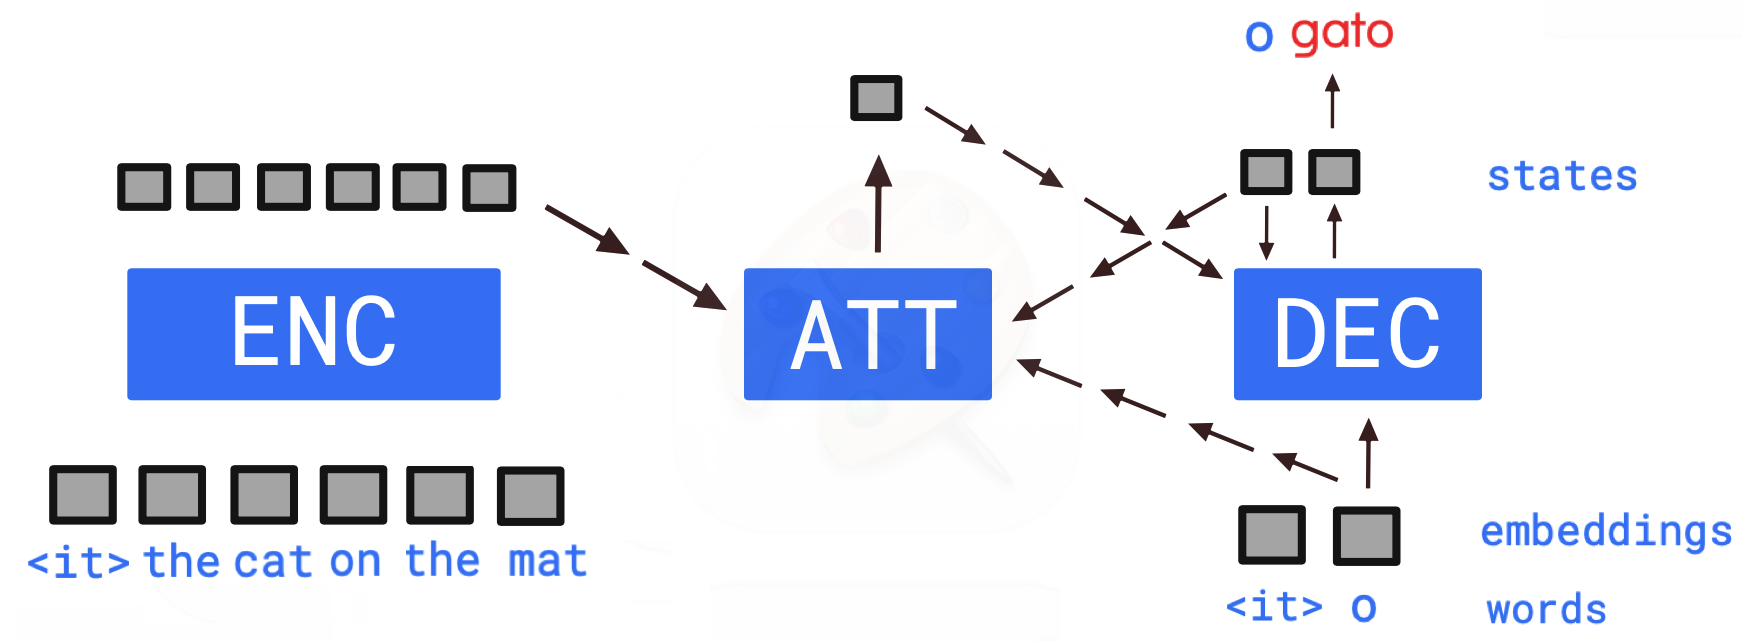
\includegraphics[width=0.8\textwidth]{textual/Figuras/enc-dec.png}
\caption{The encoder-decoder-attention NMT architecture, based on an illustration by~\textcite{lakew2019multilingual}. The \emph{encoder} reads the input sentence (``the cat on the mat'') word by word. For each word, it creates a state capturing its meaning. The \emph{decoder} then builds the translated sentence (``o gato'') one word at a time. To do this, it considers the previous word (``o''), its own internal state, and a special \emph{attention} mechanism. Attention allows the decoder to focus on relevant parts of the encoder's states (e.g., ``cat'') to generate the correct translation (``gato'').}
\label{fig: Encoder-decoder-attention} 
\end{figure}

As \textcite{lakew2019multilingual} explains, the core of NMT lies in how the encoder and decoder work together. The encoder acts like a translator, mapping the source sentence into a sequence of state vectors that capture each word's meaning and its connection to others. The decoder then builds the target language word by word, relying on three key elements: its internal memory of previously translated words, the last generated word for fluency, and the ingenious attention mechanism \parencite{luong2015effective}. This mechanism acts like a filter, highlighting the most relevant parts of the encoded source sentence for each target word, allowing the decoder to translate complex sentences.

Pioneering NMT approaches (like those by \textcite{sutskever2014sequence}) rely on recurrent neural networks (RNNs) to analyze the source sentence word by word. Stacking multiple RNN layers creates ``deep'' recurrent NMT, enabling them to capture some context within the sentence. However, these models still struggle with long-range dependencies, meaning they can have difficulty understanding how words far apart in the sentence relate to each other, particularly in complex sentences. Despite their theoretical flexibility, RNN-based NMT can be challenging and slow to train \parencite{lakew2019multilingual}.

Transformer-based NMT systems, introduced by~\textcite{Vaswani-2017}, takes a fundamentally different approach. They leverage a transformer architecture that analyzes the entire source sentence at once using an attention mechanism. This is in contrast to recurrent NMT, which processes information sequentially. By analyzing the entire sentence at once, transformers can effectively capture long-range dependencies between words, leading to generally more parallelization and better translation quality compared to recurrent NMT.

\begin{figure}[ht]
\centering
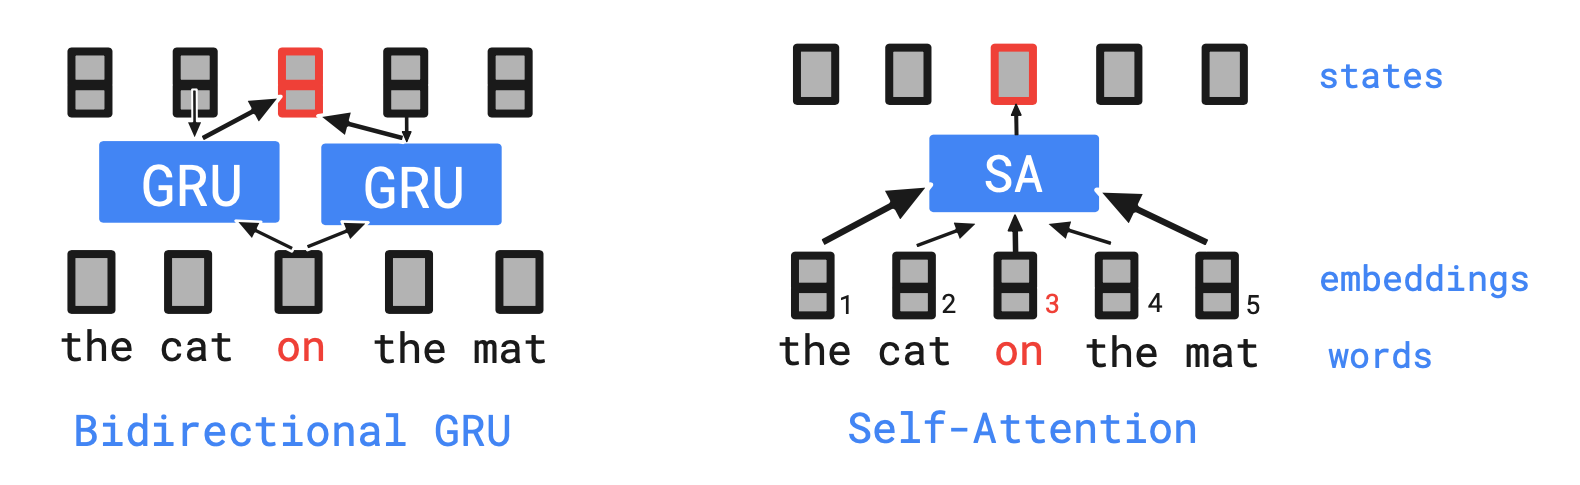
\includegraphics[width=0.9\textwidth]{textual/Figuras/self.png}
\caption{How Encoders Read Sentences: Recurrent vs. Transformers (based on \textcite{lakew2019multilingual}).}
\label{fig: rnn-transformers} 
\end{figure}

Figure~\ref{fig: rnn-transformers} depicts the differing approaches of RNNs, such as LSTMs, and transformers within NMT encoders when handling sentences. RNNs (on the left) process words sequentially, like building blocks (e.g., ``the'' then ``cat''). Here, two processing units (``GRU'') create the state for ``on''. In contrast, transformers (on the right) analyze all words at once (``the'', ``cat'', ``on''). They use a self-attention mechanism (marked by SA) to understand word order and create the state for ``on''. This parallel processing allows transformers to work more efficently than RNNs, leading to better results in NMT.

In essence, the potency of the transformer, as detailed in~\textcite{lakew2019multilingual}, stems from its architecture built upon a series of ``encoder-decoder layers'' operating in an autoregressive manner. This means it relies on the previously generated element to predict the next one, analyzing information step-by-step. Notably, both the encoder and decoder can consist of identical layers, each containing two sub-layers: a multi-head ``self-attention'' mechanism and a position-wise ``feed-forward'' network. The first highlights the most important connections between words within the sentence, while the second adds extra processing power for deeper analysis. However, the decoder incorporates an additional multi-head attention layer that allows it to focus on the outputs generated by the encoder. This multi-head attention mechanism effectively enables the use of multiple attention functions while maintaining similar computational costs to a single attention function, ensuring coherent and accurate translation.


\subsection{A Promising Approach with Emerging Limitations}

A decade after publishing his seminal work on ``Statistical Machine Translation,'' \textcite{koehn2020neural} revisits the field in ``Neural Machine Translation,'' highlighting a dramatic shift in translation technology. Deep learning architectures, particularly neural networks, have become the dominant paradigm. As the author points out, this shift has brought impressive improvements in translation quality, but also introduced new challenges.

One major hurdle for NMT is \textit{domain mismatch}. As highlighted by~\textcite{koehn-knowles-2017-six}, NMT systems often struggle when translating text from specific domains that differs significantly from the data they were trained on. This is because these specialized domains have unique vocabulary and phrasings that may be uncommon in general training data. In such cases, NMT models can prioritize accuracy over idiomacity, resulting in translations that sound grammatically correct but miss the intended meaning. 

An interesting approach to address this challenge involves domain adaptation. Here, a customized version of the model is further refined by training it on additional data from the target domain for a shorter period. This two-step process, championed by~\textcite{LuongPM15, FreitagA16}, leverages the strengths of both general and domain-specific training data. This can lead to more accurate use of terminology in NMT, particularly for specialized domains like legal documents or medical reports \parencite{matusov-etal-2019-customizing, mirkin2015personalized}.

Furthermore, NMT exhibits a ``steeper learning curve'' compared to SMT when it comes to the \textit{amount of training data} required. In simpler terms, NMT models need significantly more data exposure to achieve good performance. Consequently, NMT excels in high-resource settings (abundant training data) but struggles with limited data, resulting in lower quality outputs (as observed by~\textcite{koehn-knowles-2017-six}). This vulnerability to data scarcity can lead to another issue -- \emph{overfitting}. Imagine a student who memorized every answer in a textbook failing to answer slightly rephrased questions. Similarly, NMT models trained on a limited dataset might do well at translating those specific sentences but struggle with entirely new vocabulary or sentence structures.

Another thing is that, while NMT excels at handling extremely \textit{low-frequency words} (e.g., proper nouns) thanks to sub-word level operations (like byte-pair encoding), a key challenge remains: translating rare words belonging to highly inflected categories (e.g., verbs). Previously, according to~\textcite{koehn-knowles-2017-six}, research suggested that NMT usually struggles with rare words in general \parencite{LuongPM15, sennrich-etal-2016-neural} due to their smaller vocabularies. However, their study comparing NMT and SMT systems of similar quality for German-English translation found that NMT actually outperforms SMT on very infrequent words.

\textit{Very long sentences} pose a particular challenge for NMT, with quality dropping significantly compared to shorter ones. This was especially true for early models \parencite{cho2014properties, pouget2014overcoming}. Interestingly, recent research suggests that a simpler factor, the mismatch between training and testing data lengths, could also contribute to this performance drop \parencite{varis-bojar-2021}. To investigate this challenge and the potential limitations of the attention mechanism, \textcite{koehn-knowles-2017-six} employed a powerful English-Spanish NMT system to translate news articles from a standard dataset. They categorized the translations by their original length in the source language and evaluated the quality for each group. While NMT generally outperformed SMT, a surprising finding emerged: for very long sentences (over 80 words), the NMT system produced significantly shorter translations, often omitting details. This suggests that the attention mechanism might struggle with capturing the full context in extremely long sentences.

According to~\textcite{koehn-knowles-2017-six}, although common in NMT, attention mechanisms may not directly map to traditional \textit{word alignment} models. Originally, the intention behind incorporating attention in NMT was to establish word alignments. This involved creating a probability distribution that assigned weights to source words based on their relevance to each target word, treating the source sentence more like a bag-of-words. Despite this initial goal, there is an argument to be made that attention in NMT does not fulfill the same role as word alignment in SMT. Unlike SMT's direct word-to-word correspondence between source and target languages, NMT's attention focuses on highlighting relevant source words for target word generation.

Lastly, \textit{beam search}, a technique for finding the best translation in both SMT and NMT, seems to have a sweet spot. While increasing the number of explored possibilities (beam size) generally improves translation quality, \textcite{koehn-knowles-2017-six} have observed a ``beam search curse''. Beyond an optimal beam size (usually around 30-50), translation quality actually worsens. This seems to be because wider beams favor shorter translations, leading to a drop in quality despite exploring more options. Techniques like score normalization by translation length can help mitigate this issue, but there is a clear limit to how much beam size can be increased for optimal NMT performance.

Overall, NMT offers a valuable tool for communication despite limitations like domain mismatch, data scarcity, and challenges with long sentences. These limitations contribute to the current focus of NMT, as argued by~\textcite[19]{koehn2020neural}, which is ``not to achieve perfect translation but to drive down error rates of machine translation systems''. This means that, while current NMT systems may not achieve perfect translations and can struggle with deeper meaning, they often generate understandable text for most audiences -- including casual users, students, and professionals -- who can handle some ambiguity.


\subsection{The Rise of Large Language Models}

LLMs, powered by the transformer architecture, have made significant strides in the field of NLP \parencite{zhao2023survey}. These complex and robust AI systems, trained on extensive datasets of text and equipped with billions of parameters, exhibit a notable ability to comprehend and respond to human language.

Models such as ChatGPT have demonstrated their capabilities in a variety of tasks. They are able to engage in conversations, understand user intent, and provide informative or helpful responses. This is due to their ability to analyze large amounts of textual data and identify patterns that resemble human conversation \parencite{yuhan-etal-2023-unleashing}. Consequently, LLMs can adjust their communication style to match the user and generate responses that are contextually relevant. This progression is similar to the transition from statistical methods to neural networks in MT, with pre-trained models paving the way for the development of more advanced LLMs over the past few years. This trend is illustrated in Figure~\ref{fig: LLM-releases}, which shows the increasing number of LLMs released.

LLMs can be generally categorized into two main types, each with a distinct approach based on its underlying architecture \parencite{yuhan-etal-2023-unleashing} (as outlined in Table~\ref{tab:pre-trained-models}). \emph{Encoder-Decoder} models, recognized for their versatility, combine an encoder that interprets the input with a decoder that generates an output based on the encoded information. This dual functionality enables them to perform well in tasks such as translation or sentence completion. On the other hand, \emph{Decoder} models specialize in generating outputs. They employ a decoder to produce text or other formats based on specific conditions or context, similar to generating text in response to prompts.

\begin{table}[htb]
\footnotesize
\centering
\begin{tabular}{lccl}
\toprule
\textbf{Model} & \textbf{Publishing Agency} & \textbf{\#Parameters} & \textbf{Architecture} \\ \midrule
T5 \parencite{JMLR:v21:20-074} & Google Brain  & 220M--11B & Encoder-Decoder \\
ERNIE-3.0 \parencite{sun-at-al-2021}  & Baidu & 10B & Encoder-Decoder \\
ERNIE-3.0 Titan \parencite{wang-at-al-2021}   & Baidu  & 260B & Encoder-Decoder \\
PaLM-2 \parencite{google_palm2_2023}  & Google & 1.04B--2.7B & Encoder-Decoder \\
GLM-130B \parencite{zeng2023glm130b}  & Zhipu.AI  & 100M-515M & Encoder-Decoder \\ 
\midrule
GPT-2 \parencite{brown-at-al-2020}  & OpenAI  & 1.5B & Decoder \\
GPT-3 \parencite{ye2023comprehensive} & OpenAI  & 2.6B--200B & Decoder \\
GPT-3.5 \parencite{lin2023comparison}  & OpenAI  & - & Decoder \\
\midrule
FLAN \parencite{wei2022finetuned}  & Google & 137B & Decoder \\
InstructGPT \parencite{ouyang2022training}  & OpenAI & 1.3B--175B & Decoder \\
PaLM \parencite{chowdhery2022palm}  & Google & 8B-540B & Decoder \\
OPT \parencite{zhang2022opt}  & Meta AI  & 6.7B--175B & Decoder \\
Bloom \parencite{workshop2023bloom}  & HuggingFace  & 560M-176B & Decoder \\
FLAN-PaLM \parencite{chung2022scaling}  & THUNLP  & 250M--11B & Decoder \\
LLaMA \parencite{touvron2023llama}  & Stanford  & 780M-65B & Decoder \\
\bottomrule
\end{tabular}
\caption{Overview of Large Pre-training Models \parencite{yuhan-etal-2023-unleashing}.}
\label{tab:pre-trained-models}
\end{table}

The conventional methods of developing dedicated systems for specific NLP tasks can be both time-consuming and resource-intensive. This has led to a new direction in research: prompt engineering \parencite{qiao-etal-2023, zhou-etal-2022-prompt}. This novel approach enables the rapid adaptation of LLMs to specific tasks, providing a more efficient and flexible alternative. Research suggests that prompting LLMs can achieve performance results that are on par with, or even exceed, those of specialized systems across various NLP tasks, including sentiment analysis and question answering \parencite{Radford2019LanguageMA}.

\begin{figure}[htb]
\centering
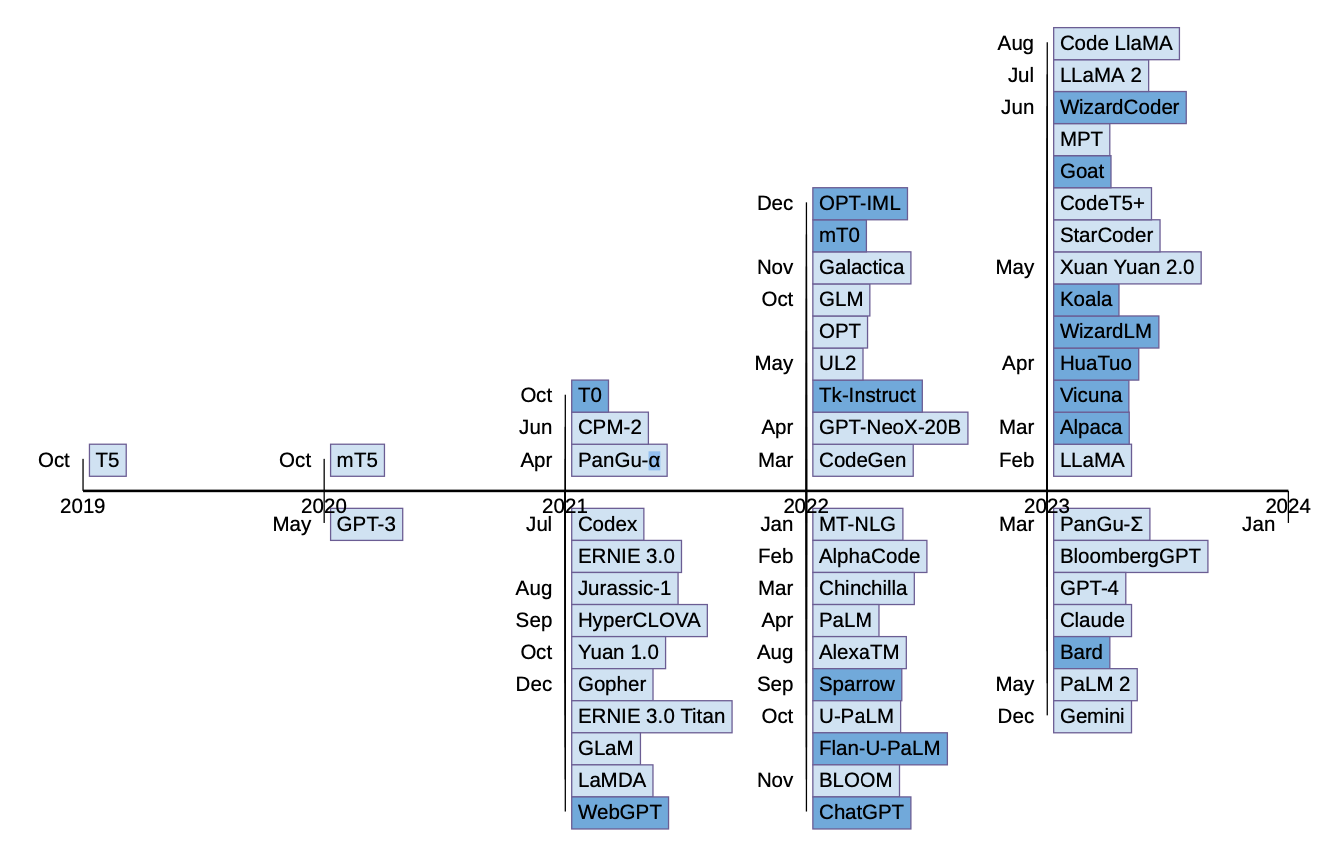
\includegraphics[width=1\textwidth]{textual/Figuras/LLM-releases.png}
\caption{Chronological LLM Release Trends, as illustrated by~\textcite{naveed2024comprehensive}. This chart shows a rise in open-source, instruction-tuned models (dark blue, top) compared to pre-trained models (light blue) and close-source (bottom). It highlights the evolving landscape of NLP.}
\label{fig: LLM-releases} 
\end{figure}

The adaptability of LLMs through prompts has significant implications for MT. \textcite{yuhan-etal-2023-unleashing} demonstrate that LLMs can achieve remarkable translation outcomes with just a few-shot translation examples, despite being trained primarily on multilingual text that is predominantly in English and not explicitly parallel (e.g., monolingual documents). This method circumvents the need for extensive parallel datasets, which are often costly and labor-intensive to produce~\parencite{garcia2023unreasonable}. However, this technique has its drawbacks. The quality of the translations is highly dependent on the example sentences used~\parencite{vilar2023prompting}. Additionally, LLM translations may sometimes introduce unnecessary or irrelevant content (overgeneration)~\parencite{bawden2023investigating}, and the computational resources required for inference can be substantial.


\subsection{The Challenges of Using LLMs}

LLMs are a game-changer in NLP, but inherent technical challenges limit their widespread application. As \textcite[30]{naveed2024comprehensive} highlights, these challenges include \emph{high computational cost}, \emph{vulnerability to manipulation} (e.g., adversarial attacks, biased inputs), and \emph{lack of explainability}. The immense computing power needed to train LLMs results in escalated production expenses and environmental impact. Additionally, the inability to understand how LLMs arrive at their outputs raises concerns about their reliability and hinders efforts to debug errors or ensure alignment with desired outcomes.

This inability to understand how LLMs arrive at their outputs (often referred to as the ``black box'' nature) hinders their application in sensitive areas, restricting their effectiveness and trustworthiness despite their impressive capabilities, as discussed by both \textcite{naveed2024comprehensive} and \textcite{yuhan-etal-2023-unleashing}. To address this issue, methodologies are being developed to make LLMs more interpretable. This transparency is crucial for fostering user trust, ensuring responsible AI development, and guaranteeing that LLMs align with human values and legal frameworks. By comprehending how LLMs reason, we can ensure they operate more ethically and responsibly.

While LLMs excel in high-resource languages, a critical challenge lies in making them more accessible and effective for \emph{low-resource languages} where data is scarce \parencite{chung2022scaling}. Research efforts are crucial to bridge this gap and ensure that users from diverse linguistic backgrounds can benefit from these models' capabilities. Additionally, LLMs can inherit and amplify societal \emph{biases} from their training data, potentially leading to ethical and \emph{fairness} issues in their outputs \parencite{naveed2024comprehensive}. Addressing these concerns is paramount for ensuring their responsible development and deployment.

Moreover, LLMs are susceptible to \emph{overfitting}. This occurs when they memorize noisy or peculiar patterns within their extensive training data, leading them to generate illogical responses when presented with unseen information \parencite{naveed2024comprehensive}. The core challenge lies in striking the right balance between \textit{memorization} and \textit{generalization}. Memorization allows the model to recall specific details from its training, ensuring accuracy for precise questions. Generalization, on the other hand, empowers the model to make inferences and respond to novel inputs, which is crucial for real-world applications. Excessive memorization can lead to overfitting, making the model inflexible and struggling with new data \parencite{naveed2024comprehensive}. Researchers are actively exploring techniques to achieve this balance, ensuring LLMs can leverage their learning power effectively.

Lastly, LLMs can exhibit ``hallucinations,'' i.e. they generate seemingly plausible but factually incorrect responses that deviate from the information given in prompts \parencite{naveed2024comprehensive}. Despite advancements, the possibility of inaccurate or nonsensical responses persists in conversational models \parencite{chung2022scaling}. To mitigate this issue, robust validation and error correction mechanisms are crucial. Additionally, as noted by the authors, LLMs should maintain contextual coherence and memory over extended dialogues, while also recognizing and addressing inconsistencies in their outputs.

\vspace{0.5em} % Adjust the value (e.g., 1em) to increase or decrease the gap

In a few words, in Section~\ref{sec: nmt}, we examined the evolving landscape of NMT by considering both its promise in addressing longstanding translation challenges and its emerging limitations. While NMT represents a significant advancement, particularly with the rise of LLMs, the complexities associated with handling diverse linguistic structures and nuances persist. This analysis sets the stage for understanding the potential and constraints of NMT systems, guiding future research and development in MT.


\section{Translation Quality Assessment}
\label{chap: tqa}

\epigraph{Quality is, I would argue, more important than it’s ever been because there are now so many critical eyes on it. \\ \hfill --- Simon Constable, Global Language Services, Visual Data}

The multifaceted nature of translation -- encompassing cognitive, linguistic, social, cultural, and technological aspects -- makes assessing its quality a complex and multidimensional task. This inherent complexity complicates the development of a single, universally accepted evaluation method. Given that a single text can often have multiple valid translations and that human evaluation is inherently subjective, the most appropriate assessment approach depends on the specific needs and context of the project. Therefore, this section aims to explore the strengths and weaknesses of both human and automatic evaluation methods, shedding light on the diverse approaches available for assessing translation quality.


\subsection{Human Evaluation}

In the realm of translation quality assessment (TQA), human evaluation remains a crucial method. Evaluators, acting as expert judges, provide their insights on the system's output. This assessment is typically conducted on a sentence-by-sentence (or ``segment-by-segment'') basis, focusing on individual segments of text. However, evaluations that encompass entire documents have also been explored, as demonstrated in \textcite{castilho-2020-page}.

Despite advancements in automatic metrics, human evaluation is still considered the gold standard. These automatic metrics are usually validated by how well they correlate with human judgments. According to \textcite{Rossi2022}, human evaluators typically judge translations using two key benchmarks: adequacy and fluency. \emph{Adequacy} measures how well the machine translation captures the original meaning (source segment), using a scale of 1 (no meaning transferred) to 4 (all meaning conveyed completely). \emph{Fluency}, on the other hand, evaluates ``the extent to which the translation follows the rules and norms of the target language'' \parencite[18]{castilho-2020-page}, that is, it assesses how natural and coherent the output sounds, independent of the source text. This metric usually uses a similar 4-point scale, ranging from nonsensical (1) to native-sounding (4). While valuable, both approaches are considered extremely time-consuming and expensive.

Another key concept in TQA is \emph{acceptability}. \textcite{Roturier2006AnII} suggests that this term goes beyond merely understanding the content in the target language. It also involves ``the manner in which its textual characteristics are going to be accepted, tolerated, or rejected by its receivers'' \parencite[66]{Roturier2006AnII}. Therefore, acceptability relates to how final users cope with, perceive, and react to the imperfections of the MT process itself. Ideally, real users would evaluate acceptability for the most accurate results. However, this can be impractical in research settings. \textcite{Rossi2022} propose alternatives to address this challenge, such as employing students or crowdsourcing platforms.

For quicker evaluations, some methods simply ask evaluators to rank the outputs of two different MT systems, essentially choosing the ``better'' option without needing specific justifications. This approach, often used by MT providers for online user feedback, allows for faster data collection, as also pointed out by~\textcite{Rossi2022}.

Apart from basic methods like spreadsheets, several advanced tools offer a more streamlined, informative, and efficient approach. One such example is KantanLQR\footnote{\href{https://kantanmt.zendesk.com/hc/en-us/articles/115003644483-What-is-KantanLQR}{https://kantanmt.zendesk.com/hc/en-us/articles/115003644483-What-is-KantanLQR}} (``Language Quality Review'') by Kantan AI, which allows users to prioritize specific quality criteria and compare outputs based on those factors. These tools go beyond simple scoring, visualizing human evaluator scores and calculating overall scores for different MT systems, thus providing valuable insights for improvement.

For a less expensive option, traditional spreadsheet programs like Google Sheets can still be used for human MT evaluation. Users can manually input scores for different quality indicators and calculate average scores. Finally, free online forms offer another approach, particularly useful for conducting surveys \parencite[58]{Rossi2022}.

Despite providing gold standard results for machine translation evaluation, human translation is not without drawbacks. One key challenge, as argued by~\textcite{Rossi2022}, is \emph{subjectivity}. Multiple evaluators may have differing opinions on the quality of a translation, even for a single source text with several valid options. This can make achieving consistent results difficult. Additionally, human evaluation is time-consuming and resource-intensive. Evaluators require training and expertise, and the process itself can be slow, especially for large volumes of text. While setting clear objectives can mitigate subjectivity, these metrics may not always capture the nuances of real-world usage \parencite{popovic-2018}.


\subsection{Manual Error Classification of Spatial Semantics}

In TQA, human experts can go beyond simply assigning scores. They can pinpoint specific errors and categorize them based on a pre-defined system. This helps diagnose issues in MT and provides valuable feedback for improvement. For this task, evaluators need the translated text along with a reference point, such as the original source text or a high-quality reference translation (or ideally both) \parencite{Rossi2022, popovic-2018}.

As MT continues to advance, human post-editing has gained popularity as a method to refine the final output generated by the MT system. This has sparked a growing interest in analyzing these edits. By assigning error categories to each correction made by human editors, researchers can explore the connections between different types of errors and the effort required for post-editing (cognitive, time-related, and technical effort, as defined by~\textcite{popovic-2018, Kittredge2002KringsHP}). Notably, for this analysis, only the post-edited translation is essential, while the original source text is not always necessary.

TQA requires defining clear error categories (i.e. an error taxonomy) and a systematic evaluation scheme for manual error classification, as depicted in Figure~\ref{fig: human-evaluation}. While seemingly straightforward, these tasks are complex. According to~\textcite{popovic-2018}, each category must reflect the strengths and weaknesses of the chosen MT systems, the translation task at hand, and the languages involved. More detailed categories can provide richer information but may be harder to distinguish consistently. Ideally, the categories should encompass both linguistic errors and broader translation issues.

\begin{figure}[htb]
\centering
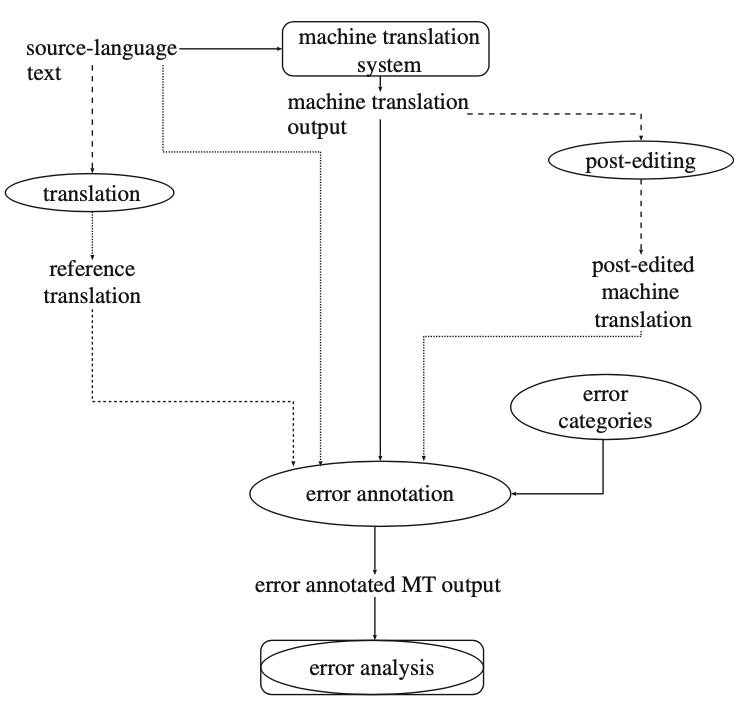
\includegraphics[width=0.7\textwidth]{textual/Figuras/human evaluation.png}
\caption{Manual Error Annotation: rectangles denote automatic processes and ellipses denote manual processes \parencite{popovic-2018}.} 
\label{fig: human-evaluation} 
\end{figure}

Frameworks like the Multidimensional Quality Metrics (MQM) offer an extensive list of error categories, which can be overwhelming \parencite{Mariana2014TheMQ}. A simpler approach, according to \textcite{Moorkens-2018}, is to use a limited set of common error types during evaluation, such as \emph{word order} mistakes (words not appearing in the correct order), \emph{mistranslations} (inaccurate or not fluent in the target language), \emph{omissions} (missing words from the source text), and \emph{additions} (words not found in the source text).

Once error categories are defined, applying them to real-world translations becomes crucial. However, as highlighted by~\textcite{Rossi2022}, it is important to note that a small sample of translated text might not be representative of an MT engine's overall performance. Ideally, human experts would evaluate multiple samples to choose the best system. But large-scale testing requires significant resources. Smaller enterprises might rely on automatic scoring, measuring the time and effort required to fix the translations (post-editing effort), or using a combination of both methods to ensure a more accurate assessment.


\subsection{Automatic Evaluation Metrics}

Automatic evaluation metrics (AEMs) offer a significant advantage over human assessment: they are considerably faster and more cost-effective. This advantage allows MT providers to perform frequent checks on the quality of their systems. According to~\textcite{Rossi2022}, AEMs are particularly useful in two key scenarios:

\begin{description}
    \item[MT Engine Development:] During the development of an MT engine, AEMs can be used to evaluate the engine's performance after each modification. This allows developers to determine if the changes have improved the engine's performance for their specific needs.
    \item[MT Option Selection:] When choosing an MT option for a project, AEMs can be employed to compare the quality of translations produced by different MT systems for the same source text. This comparison helps users select the most suitable MT system for their project requirements.
\end{description}

It is important to acknowledge that human translators often produce different, yet valid, translations for the same source text. As a result, we cannot expect an MT system to perfectly match a human translation. However, the closer a machine translation is to a human translation, the generally better it is considered to be \parencite{Rossi2022}. Many AEMs are built on this principle of similarity. These tools compare the MT output (called the \emph{candidate translation} or \emph{hypothesis}) to a human-generated ``gold standard'' or \emph{reference translation} to calculate scores. Some AEMs can even be incorporated with multiple reference translations to account for natural variations in human translation.

While AEMs are valuable for MT evaluation, \textcite{koehn2020neural} highlights a tension between the trust researchers place in these metrics and the ongoing debate about their true effectiveness in assessing MT quality. While AEMs heavily influence system design due to their focus on score optimization, researchers acknowledge their limitations and frequently challenge their validity. 


\subsubsection{Core concepts: \emph{n}-grams, precision, recall and F-measure}

This subsection introduces four core concepts: \emph{n}-grams, precision, recall, and F-measure, which form the building blocks of the more elaborate AEMs presented subsequently.

\subsubsection{\emph{n}-grams}

\emph{n}-grams, sequences of \emph{n} words, are a fundamental concept in many AEMs. In simpler terms, they represent groupings of consecutive words in a text. For instance, in the sentence ``He swam across the river,'' ``he'' is a unigram (1-gram), ``he swam'' is a bigram (2-gram), and ``he swam across'' is a trigram (3-gram). Similarly, 4-grams, 5-grams, and so on can be formed by extending the sequence length.

According to \textcite{Rossi2022}, \emph{n}-grams play a vital role in language modeling, where they estimate the probability of a word appearing based on the preceding \emph{n}-words. For example, in metrics such as BLEU, a trigram probability might indicate the likelihood of encountering a specific word given the two words before it in a sentence.

In the context of AEMs, \emph{n}-grams are typically sequences of \emph{n} words in the candidate translation that also exist in the reference translation. This essentially compares the overlap between the candidate translation and the human-generated ``gold standard'' translation. It is important to note that recent advancements have led to AEMs that consider character sequences instead of words. In these cases, \emph{n}-grams refer to sequences of \emph{n} characters rather than \emph{n} words.


\subsubsection{Precision and Recall}

Precision and recall are fundamental concepts in NLP. \textcite{Rossi2022} illustrate these concepts with a simple example. Imagine a teacher asks a student to name the days of the week in English. The student replies with ``Monday, Tuesday.'' This student provided two correct answers and no incorrect ones. \emph{Precision}, which measures the ratio of correct answers to the total number provided, would be a perfect score of 100\% (two out of two). However, from the teacher's perspective, the answer is incomplete. The teacher knows there are seven days in a week, and the student omitted five of them. This highlights the concept of \emph{recall}, which refers to the ratio of correct answers provided to the total number of correct answers possible (in the ideal response). In this case, the student's recall score would be two out of seven, which is roughly 29\%.

In the context of AEMs, precision focuses on the ratio of correct words in the candidate translation; that is, those that also appear in the reference translation, to the total number of words in the candidate translation. Mathematically, it can be expressed as:

\begin{equation}    
 \text{precision of \emph{C}} = \frac{\text{no. of correct words in \emph{C}}}{\text{no. of words in \emph{C}}} \hspace{1cm}
\end{equation}

where \emph{C} is the candidate translation.

Recall, on the other hand, focuses on the ratio of correct words in the candidate translation to the total number of words in the reference translation. It essentially measures how well the candidate translation captures everything from the reference. Mathematically:

\begin{equation}    
 \text{recall of \emph{C}} = \frac{\text{no. of correct words in \emph{C}}}{\text{no. of words in \emph{R}}} \hspace{1cm}
\end{equation}

where \emph{C} is the candidate translation, and \emph{R} is the reference translation.

\subsubsection{F-measure}

The example with the days of the week by~\textcite{Rossi2022} highlights the trade-off between precision and recall. To prioritize precision, the student could withhold further answers after ``Monday, Tuesday'' to avoid potential mistakes. Conversely, prioritizing recall might lead them to list numerous answers, hoping some are correct. For instance, they might reply with ``Monday, Tuesday, Wednesday, Thursday, Friday, Saturday, Sunday, January, February, March, April, May, June, July, August, September, October, November, December.'' While their recall would soar to 100\% (7 out of 7 correct days), precision would plummet below 37\% (7 correct answers out of 19 total). Neither strategy is ideal from the teacher's perspective.

The F-measure seeks to balance precision and recall by calculating their harmonic mean. Mathematically, it is defined as:

\begin{equation}
\text{F-measure} = 2 \times \frac{\text{precision} \times \text{recall}}{\text{precision} + \text{recall}}
\end{equation} \break

which can also be reformulated as:

\begin{equation}
\text{F-measure} = 2 \times \frac{\text{no. of correct words in \emph{C}}}{\text{no. of words in \emph{C}} + \text{no. of words in \emph{R}}}
\end{equation} \break


The F-measure penalizes extreme values in either precision or recall, favoring outputs that achieve a balance between the two. 


\subsubsection{BLEU}

Traditional evaluation methods like word error rate (common in speech recognition) struggle with correctly evaluating MT outputs. These methods miss the subjectivity of translation and the importance of word order in conveying meaning. To address these limitations, IBM’s BLEU (Bilingual Evaluation Understudy) was developed as a more comprehensive approach to automatic evaluation \parencite{papineni-etal-2002-bleu}

BLEU goes beyond simple word matching. It analyzes \emph{n}-grams (sequences of words up to 4 words long) in both the MT output and reference translations. By comparing the number of matching \emph{n}-grams and their order, BLEU rewards translations that preserve the original structure. Essentially, it is a precision metric focusing on the proportion of \emph{n}-grams in the MT output that also appear in the reference(s). The overall BLEU score is calculated as a geometric mean of individual \emph{n}-gram precisions  \parencite{koehn2020neural}.

While BLEU allows for multiple reference translations for flexibility, it emphasizes precision through a \emph{brevity penalty}. This discourages excessively short translations by penalizing outputs with a lower word count than the reference. The BLEU score itself is a combination of this penalty and a weighted sum of \emph{n}-gram precisions (ratio of matching n-grams in the machine translation to the reference(s)). Although using multiple references is less common now, it remains a valuable option.

The formula for BLEU, as defined in \textcite{koehn2020neural}, is presented below:

\begin{equation}
    \text{BLEU} = \text{BP} \times \exp \sum_{n=1}^{4} \log \left( \frac{\text{matching \emph{n}-grams}}{ \text{total \emph{n}-grams in machine translation}} \right) 
\end{equation}

\begin{equation}
    \text{BP} = \text{min} \left(1, \frac{\text{output-length}}{\text{reference-length}} \right)
\end{equation}

Here, BP represents the brevity penalty.

It is important to acknowledge that BLEU is a valuable tool, but not a perfect replacement for human evaluators. As highlighted in \textcite{koehn2020neural}, it has limitations:

\begin{description}
    \item[Ignores Word Importance:] 
    BLEU assigns equal weights to all words in a sentence, even though some words like ``not'' or proper nouns hold greater meaning compared to determiners (``the'', ``a'') or punctuation.
    \item[Overlooks Grammar:] BLEU focuses on matching \emph{n}-grams from the generated text to the references. This can lead to high scores for nonsensical sentences with the right \emph{n}-grams, but lacking overall grammatical correctness. 
    \item[Meaningless Scores:] BLEU scores are sensitive to factors like the number of reference translations, language pair, and even word segmentation. This makes interpreting scores (e.g., 30\%) and comparing translations across settings difficult.
    \item[Low Human BLEU Scores:] Experiments show that human translations compared against each other using BLEU still score relatively low. This suggests BLEU might not capture the full complexity of good human translation.
\end{description}


In essence, the critique argues that BLEU is a flawed metric because it does not reflect the true quality of an automatic translation. It might favor translations with matching \emph{n}-grams but poor grammar or miss important nuances that affect meaning.


\subsubsection{METEOR}

Evaluating MT accuracy often relies on surface-level comparisons between the candidate texts and human references. This approach can be misleading, as changes in wording or sentence order might not affect the core meaning. Simple evaluation metrics often penalize such variations, leading to inaccurate assessments \parencite{koehn2020neural}.

While traditional metrics like BLEU focus on surface-level \emph{n}-gram matching, METEOR tackles this limitation by incorporating semantics through stemming and synonyms. Stemming recognizes that words with the same root carry similar meaning (e.g., ``responsibility'' and ``responsible'' are both stemmed to ``respons''). METEOR also considers synonyms as valid matches, understanding that translators might choose ``security'' or ``safety,'' or ``responsibility'' or ``charge,'' without affecting the core meaning \parencite{koehn2020neural}. 

To evaluate a translation, METEOR employs a multi-step matching process, first attempting exact word matches and then considering stemmed forms or synonyms using WordNet synsets \parencite{saadany-orasan-2021-bleu, pedersen-etal-2004-wordnet}.

METEOR first calculates unigram precision and recall. Then, a harmonic mean (F-mean) is computed. This metric emphasizes recall, placing more weight on capturing all correct words from the reference:

\begin{equation}
\text{F-mean} =  \frac{10 \times (\text{precision} \times \text{recall})}{9 \times \text{recall} + \text{precision}}
\end{equation} 

While METEOR's core scoring focuses on unigram matches, it goes a step further by penalizing translations that significantly alter the word order. This discourages translations that capture meaning but severely mangle sentence structure \parencite{banerjee-lavie-2005-meteor}

METEOR assesses word order preservation by analyzing how well mapped words (between translation and reference) are grouped together. Ideally, these mapped words should appear consecutively in both texts (fewer chunks). The more scattered these mapped words are (more chunks), the higher the penalty. This penalty is calculated as:

\begin{equation}
\text{Penalty} = 0.5 \times \frac{\text{\# chunks}}{\text{\# unigrams-matched}}
\end{equation} 

For instance, with a candidate translation of ``the president spoke to the audience'' and a reference of ``the president then spoke to the audience,'' there are two chunks (``the president'' and ``spoke to the audience''), resulting in a penalty. The penalty increases with more chunks (up to a maximum of 0.5), and decreases with fewer chunks (minimum depends on matched unigrams) \parencite[68]{banerjee-lavie-2005-meteor}.

Finally, the METEOR score combines the F-mean and the penalty, with a higher penalty for poorer word order preservation. For multiple reference translations, METEOR picks the best score after evaluating against each. The overall system score is obtained by aggregating statistics across the entire test set.

\begin{equation}
\text{METEOR} = \text{F-mean} \times (1 - \text{Penalty})
\end{equation} 

While METEOR offers a more nuanced evaluation than BLEU, \textcite{koehn2020neural} emphasizes it comes with added complexity. METEOR requires resources like stemmers and synonym databases, which can be computationally expensive. The matching process involves aligning words between the MT output and the reference translation, adding further computational overhead. Additionally, METEOR has several parameters that need to be fine-tuned for optimal performance, such as the weight given to recall versus precision or the importance of stemming and synonym matches.

In essence, METEOR offers a more sophisticated approach to MT evaluation by considering semantic relationships between words. However, its increased complexity requires careful consideration of computational resources and parameter optimization.


\subsubsection{BERTScore}

Traditional metrics like BLEU and METEOR rely on \emph{n}-gram matching, focusing on surface-level similarities between the candidate text and a reference. This approach often disregards the deeper meaning, particularly when it comes to paraphrases. For example, as \textcite{saadany-orasan-2021-bleu} point out, these metrics might score ``people like visiting places abroad'' higher than ``consumers prefer imported cars,'' even though both may convey the same preference for foreign things in different words.

Newer approaches address this limitation by leveraging pre-trained language models like BERT. BERTscore \parencite{zhang2020bertscore} exemplifies this approach. It calculates a score based on the similarity in contextual meaning between each word in the translation and the reference. By using contextual embeddings, similar to how humans understand language, BERTScore captures the meaning of each word in relation to others. This allows it to accurately assess paraphrases and even distant dependencies in word order, such as the difference between ``A because B'' and ``B because A.'' These capabilities lead to a more accurate and comprehensive evaluation that considers both meaning and structure.

BERTScore evaluates the similarity between a reference (denoted by $x = ⟨x_1, ..., x_k⟩$) and a candidate (denoted by $\hat{x} = ⟨\hat{x}_1, ..., \hat{x}_l⟩$) using contextual embeddings and cosine similarity. These embeddings capture the meaning of each word based on its surrounding context. Figure~\ref{fig: bertscore} illustrates the computation. Optionally, inverse document frequency (idf) scores can be incorporated to emphasize the importance of rare words.

\begin{figure}[htb]
\centering
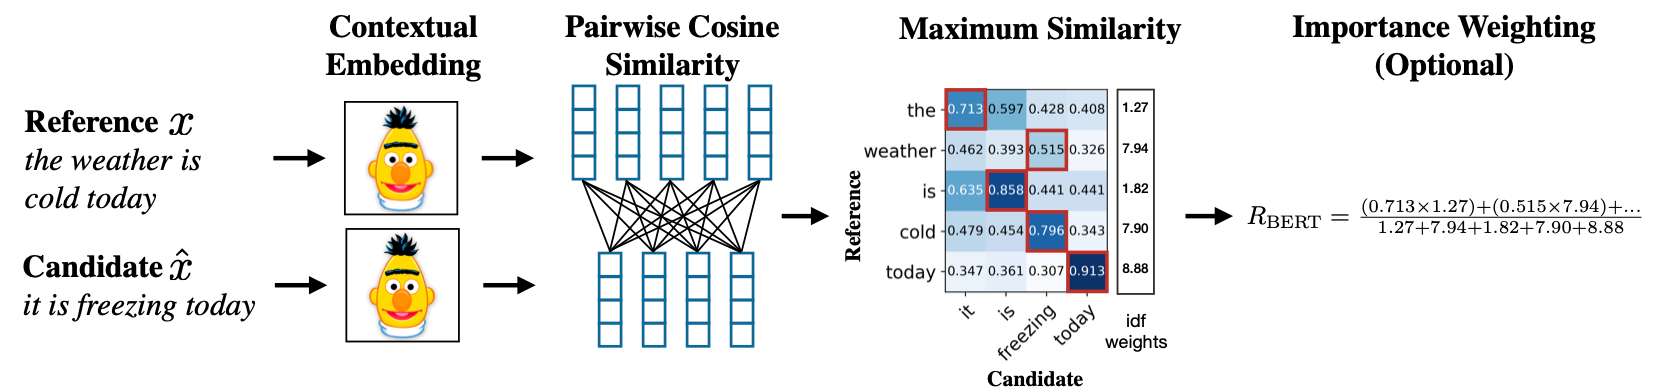
\includegraphics[width=1\textwidth]{textual/Figuras/bertscore.png}
\caption{BERTScore Recall ($R_{BERT}$) computation. Shows BERT embeddings, cosine similarity for all word pairs (lines), greedy matching (red arrows), and optional idf weighting \parencite{zhang2020bertscore}.} 
\label{fig: bertscore} 
\end{figure}

Key Components of BERTScore \parencite{zhang2020bertscore}:

\begin{description}
    \item[Contextual Embeddings:] To generate contextual embeddings, BERTScore utilizes models like BERT \parencite{devlin-etal-2019-bert} or ELMO \parencite{peters-etal-2018-deep} to represent tokens in the input sentences $x$ (reference) and $\hat{x}$ (candidate). These embeddings use vector representations to capture the meaning of a word based on its surrounding context, allowing for more nuanced comparisons than traditional word embeddings that only consider the word itself.
    \item[Similarity Measure:] Instead of exact string matching, BERTScore employs cosine similarity to measure the similarity between a reference and a candidate sentence. Cosine similarity calculates the angle between two vectors, with a higher value indicating greater similarity. In BERTScore, the cosine similarity of a reference token $x_i$ and a candidate token $\hat{x}_j$ is is calculated is calculated using their pre-normalized embedding vectors: $x_i \boldsymbol{\top} \hat{x}_j$. While this measure considers tokens in isolation, the contextual embeddings inherently contain information about the surrounding context, allowing for scoring even when paraphrases or different word choices are used.
    \item[Greedy Matching:] BERTScore uses greedy matching to find the most similar word in the candidate sentence ($\hat{x}_j$) for each word in the reference sentence ($x_i$). This matching helps calculate two key metrics: recall and precision. Recall measures how well it finds all the words from the reference sentence in the candidate sentence. Precision measures how accurate those matches are (avoiding extra, irrelevant words in the candidate sentence). Recall and precision are calculated as shown in Equations~\ref{r-p-bert}.
\end{description}

    \begin{equation} \label{r-p-bert}
    R_{BERT} = \frac{1}{|x|} \sum_{x_i∈x} \max_{\hat{x}_j∈\hat{x}} \left(\boldsymbol{x}_i \top \hat{\boldsymbol{x}}_j \right),
     P_{BERT} = \frac{1}{|\hat{x}|} \sum_{\hat{x}_i∈\hat{x}} \max_{x_j∈x} \left( \boldsymbol{x}_i \top \hat{\boldsymbol{x}}_j \right) \\
    \end{equation}
    
\begin{description}       
    \item[F1 Score:] BERTScore combines precision (percentage of relevant tokens matched) and recall (percentage of reference tokens found) to create an F1 score, providing a balanced measure of performance. F1 score is calculated as in Equation~\ref{f-bert}.
\end{description} 

    \begin{equation} \label{f-bert}
    F_{BERT} = 2 \times \frac{P_{BERT} \cdot R_{BERT}}{P_{BERT} + R_{BERT}}
    \end{equation}
    
\begin{description}     
    \item[Importance Weighting (Optional)]: BERTScore can optionally incorporate inverse document frequency ($idf$) scores to emphasize the importance of rare words in determining sentence similarity. Given $M$ reference sentences $\left\{{x^{(i)}} \right\}_{i=1}^{M}$, the idf score of a word-piece token $w$ is defined by Equation~\ref{idf}.
\end{description} 

    \begin{equation} \label{idf}
    idf(w) = - \log \frac{1}{M} \sum_{i=1}^{M} \mathds{1} [w∈x^{(i)}],
    \end{equation}

\begin{description}    
    \item[\hspace{=2em}]where, $\mathds{1}[\cdot]$ is an indicator function. The full $td-idf$ measure is not used because single sentences are processed, where the term frequency ($tf$) is likely 1. For example, recall with $idf$ weighting is as in Equation~\ref{r-bert-idf}:
\end{description}

    \begin{equation} \label{r-bert-idf}
     R_{BERT} = \frac{\sum_{x_i \in x} \text{idf}(x_i) \max_{\hat{x}_j \in \hat{x}} \left( \boldsymbol{x}_i \top \hat{\boldsymbol{x}}_j \right) }{\sum_{x_i \in x} \text{idf}(x_i)} \\
    \end{equation}
    
\begin{description}    
    \item[\hspace{=2em}]Because references are used to compute idf, the scores remain the same for all systems evaluated on a specific test set. Then, plus-one smoothing is applied to handle unknown word pieces.
\end{description}
    
\begin{description}    
    \item[Baseline Rescaling:] Pre-normalized vectors are used, so computed scores have the same numerical range of cosine similarity (between −1 and 1). However, to improve readability, BERTScore rescales its scores to a range between 0 and 1, considering the typical score distribution for low-similarity sentence pairs, using Equation~\ref{r-bert-baseline}.
\end{description}    

    \begin{equation} \label{r-bert-baseline}
     \hat{R}_{BERT} = \frac{R_{BERT} - b}{1 − b}
    \end{equation}

\begin{description}    
    \item[\hspace{=2em}]After applying the formula, $\hat{R}_{BERT}$ is typically between $0$ and $1$. The same rescaling procedure is done with $\hat{P}_{BERT}$ and $\hat{F}_{BERT}$.
\end{description}    


Despite outperforming \emph{n}-gram based BLEU in many scenarios, BERTScore's effectiveness can vary depending on specific elements within the text, particularly function words, as discussed by~\textcite{hanna-bojar-2021-fine}. This leads it to struggle with slight phrasing variations, such as tag questions (e.g., ``You're crazy, aren't you?'') and other nuanced linguistic features. Furthermore, BERT-based metrics like BERTScore have difficulty differentiating between incorrect translations that closely resemble the reference and more accurate ones with different wording, especially when stylistically similar.

Adding to these limitations, \textcite{sun-etal-2022-bertscore} identified a concerning bias (i.e., race, gender, religion, physical appearance, age, and socioeconomic status) in pre-trained metrics like BERTScore. These metrics exhibit significantly higher bias on sensitive attributes like gender compared to traditional \emph{n}-gram based metrics. For example, gender bias resulted in score differences of $7$-$21$ points for BERT-based metrics, whereas traditional metrics showed minimal bias ($< 1.3$ points). This might be due to how datasets are constructed for evaluation, inadvertently including stereotypes present in source data.


\subsubsection{COMET}

The recent surge in research on using neural networks to train MT models has led to significant improvements in MT quality. However, evaluating these systems has not kept pace. As pointed out by \textcite{ma-etal-2019-results, rei-etal-2020-comet}, existing AEMs still have weaknesses. For example, they might disagree with human judgments on individual sentences and struggle to distinguish between the very best performing MT systems.

COMET (Crosslingual Optimized Metric for Evaluation of Translation) \parencite{rei-etal-2020-comet}, offers a new approach to MT evaluation. This framework, built with PyTorch, trains multilingual models to assess translation quality. Inspired by recent work in Quality Estimation (QE) that showed promise in evaluating translations without a perfect reference, COMET incorporates the source language text itself. This approach differs from traditional AEMs, which typically rely solely on a reference translation for comparison.

COMET offers two distinct model architectures, as illustrated in Figure\ref{fig: comet}, to address different aspects of MT evaluation:

\begin{figure}[htb]
\centering
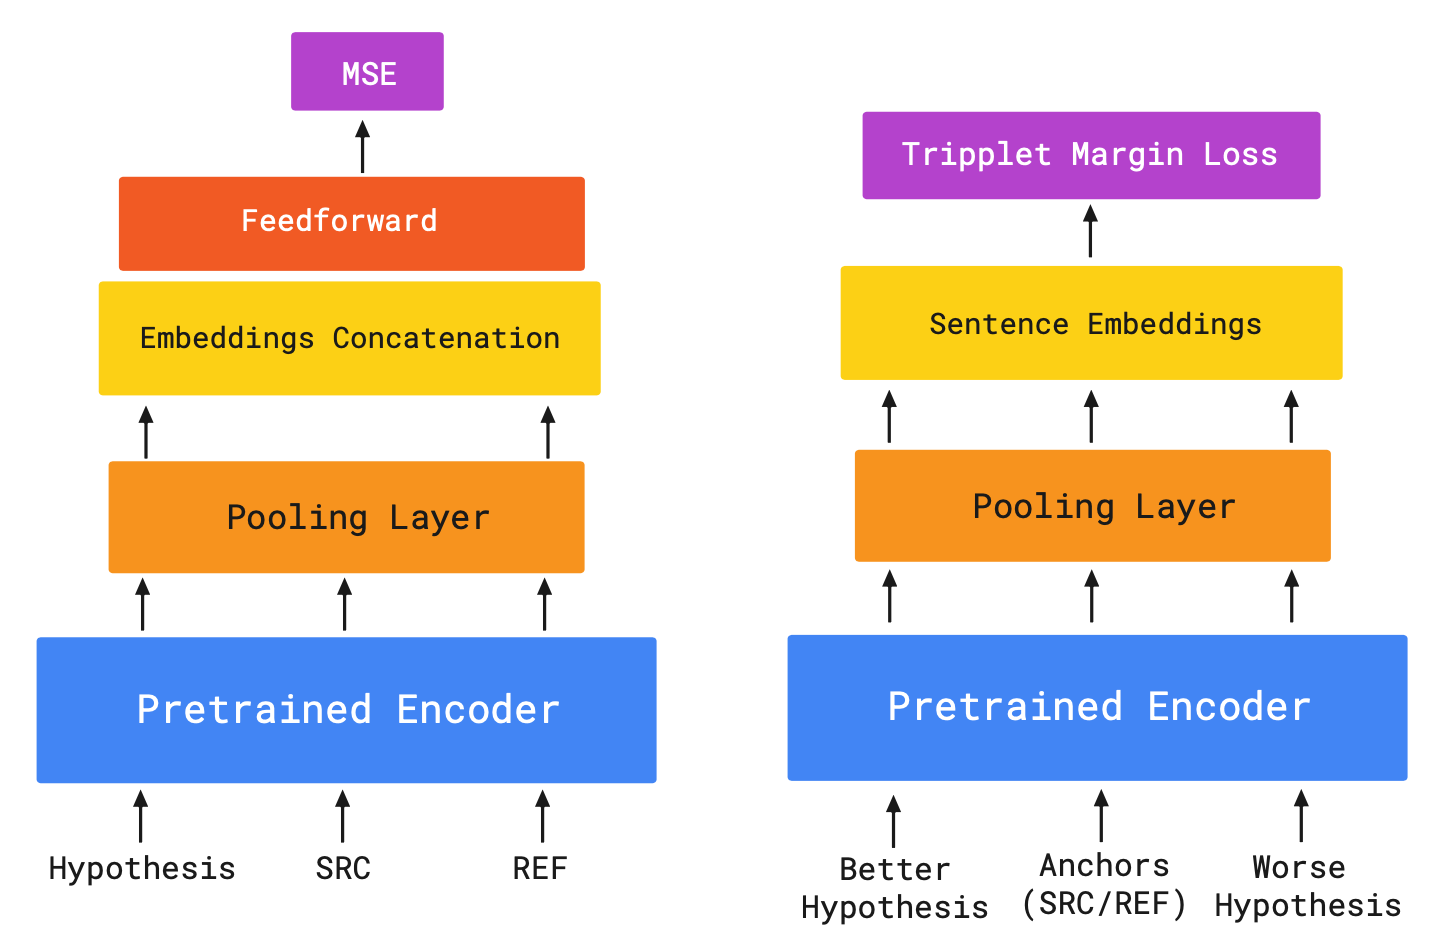
\includegraphics[width=.8\textwidth]{textual/Figuras/comett.png}
\caption{Estimator Model (left): Analyzes source text, translated text (hypothesis), and reference (optional) using a multilingual encoder. It captures the essence of each sentence (embedding) and combines this information (if a reference exists) through concatenation. Finally, it learns from human quality ratings (DA, HTER, or MQM) to predict a score for the translation via a feed-forward regressor, minimizing the Mean Squared Error (MSE). Translation Ranking Model (right): Focuses on relative quality comparison between translations of the same source text. Similar to the Estimator model, it analyzes them using a multilingual encoder to generate embeddings. During training, the model utilizes triplet margin loss to position these embeddings in the embedding space. The ``better'' translation's embedding should be closer to both the source text and the reference (if available) compared to the ``worse'' translation's embedding. This helps COMET distinguish high-quality translations \parencite{rei-etal-2020-comet}.}


\label{fig: comet} 
\end{figure}

\begin{description}    
    \item[Estimator model] (Figure\ref{fig: comet} -- on the left): This model is directly trained to predict a quality score for a given translation.
    \begin{description}
        \item \emph{Cross-lingual Encoder}: This is the foundation of both models. It utilizes a pretrained, cross-lingual model like multilingual BERT \parencite{devlin-etal-2019-bert}, with multiple transformer encoder layers, to analyze the source text, translated text (hypothesis), and reference translation (if available). The encoder considers the relationships between words within each text.
        \item\emph{Pooling Layer}: This layer combines the information from each word embedding generated by the encoder, not just the last one, to create a single embedding for each sentence. This is shown to increase model performance on MT evaluation tasks \parencite{zhang2020bertscore}. This embedding is computed as in Equation~\ref{embeding}:
            \begin{equation} \label{embeding}
            \mathbf{e}_{x_j} = \mu \mathbf{E}_{x_j}^\top \boldsymbol{\alpha}
            \end{equation}
        where, $\mathbf{e}_{x_j}$ is the embedding vector for token x, $\mu$ is the weight coefficient (scalar), $\mathbf{E}_{x_j}$ is the matrix containing layer embeddings for token x (j-th row corresponds to layer l) and $\alpha$ is the trainable weight vector corresponding to layer-wise importance (one weight per layer).
        \item\emph{Embedding Concatenation}: When the Estimator model has a reference translation, it creates embeddings for the source text, hypothesis, and reference. Concatenation simply combines these embeddings into a single list, allowing the model to consider all the information together.
        \item\emph{Feed-forward Regressor}: The sentence embeddings from the source, hypothesis, and reference (if available) are combined and fed into this layer. The regressor is trained to minimize the Mean Squared Error (MSE) between the predicted scores and human quality assessments (DA, HTER, or MQM).
    \end{description}
    \item[Translation Ranking model] (Figure\ref{fig: comet} -- on the right): focuses on learning the relative quality between different translations for the same source text. 
    \begin{description}
        \item\emph{Similar to the Estimator model}: This model also utilizes a cross-lingual encoder and pooling layer to generate sentence embeddings.
        \item\emph{Triplet Margin Loss}: During training, the model is presented with three translations for the same source text: a ``better'' translation, a ``worse'' translation, and optionally, a reference translation. Triplet margin loss encourages the model to position these embeddings in a way that reflects their quality. Ideally, the ``better'' translation's embedding should be closer to both the source text and the reference translation (if available) compared to the ``worse'' translation's embedding. This helps the model learn to distinguish between higher and lower quality translations.
    \end{description}
\end{description}

While COMET has proven effective in translation evaluation, it is not without limitations. Studies by \textcite{glushkova2023bleu} highlight specific error types that COMET struggles with. These include discrepancies in numbers between the source text and translation, mistranslated or missing named entities, unintended omissions of important content, and unnecessary insertions of words not present in the original text. These challenges have been echoed in other research \parencite{amrhein-sennrich-2022-identifying, alves-etal-2022-robust}. Attempts to address these issues using data augmentation techniques have shown some improvement \parencite{alves-etal-2022-robust}, but the gains appear to be modest.


\subsubsection{TER}

The translation error rate (TER), also known as translation edit rate, is a metric that goes beyond simple word-level accuracy and takes into account the order of words in a sentence. It builds upon the concept of word error rate (WER), a metric borrowed from speech recognition, which leverages the \emph{Levenshtein distance} to determine the minimum number of editing steps (insertions, deletions, substitutions) needed to transform one sequence of words into another \parencite{snover-etal-2006-study, koehn2012statistical}.

The Levenshtein distance can be thought of as measure of editing effort. WER takes this effort and compares it to the length of the correct translation (reference). This gives us an error rate as a percentage. A perfect translation scores 0\%, while a completely scrambled sentence scores 100\%.

Mathematically, the formula for WER is:

\begin{equation}
\text{WER} = \frac{\text{substitutions} + \text{insertions} + \text{deletions}}{\text{reference-length}}
\end{equation} 

Here, ``reference-length'' is the number of words in the reference translation.

WER treats each word move (or where a sequence of words is shifted elsewhere in the sentence) as two errors (one deletion and one insertion). This can lead to an inflated error rate for translations where the overall meaning is preserved but word order is shuffled \parencite{Rossi2022}.

TER addresses this limitation by introducing a ``shift'' operation. This means that moving any sequence of words counts as only one error, providing a more accurate reflection of errors that impact meaning:

\begin{equation}
\text{TER} = \frac{\text{shifts} + \text{substitutions} + \text{insertions} + \text{deletions}}{\text{reference-length}}
\end{equation} 

\textcite{koehn2020neural} highlights a major issue with using WER for MT. Here is an example:

\begin{boxK}
    \textbf{Hypothesis}: A spokesperson announced today: “The plan will go forward.” \\
    \textbf{Reference}: “The plan will go forward,” a spokesperson announced today.
\end{boxK}

WER harshly penalizes reordered sentences by treating the movement of the entire main clause (``A spokesperson announced today'') as separate deletion (4 errors) and insertion (another 4 errors) for a 9-word sentence, leading to an excessively inflated error rate. In contrast, TER considers such movement a single shift'' error, resulting in a much more accurate and reasonable score of just 1/9 ≈ 11\% for our example.

TER scores are not only easier to understand but also a superior metric for evaluating individual sentences. BLEU score calculation involves 4-gram precision, but a translated sentence might lack any matching 4-grams, leading to a BLEU score of 0. While TER is not as widely adopted as BLEU, it is a more suitable option for sentence-level evaluation.

Algorithm~\ref{alg:ter} calculates the minimum number of edits (shifts, substitutions, insertions, and deletions) required to transform a translated sentence (hypothesis) into a correct reference sentence as in~\textcite{snover-etal-2006-study}.

\bigskip 

\begin{algorithm}
\small
\caption{Calculate Number of Edits}\label{alg:ter}
\hspace*{\algorithmicindent} \textbf{Input:} HYPOTHESIS $h$ \\ 
\hspace*{\algorithmicindent} \textbf{Input:} REFERENCES $R$
\begin{algorithmic}
\State $E\gets∞$ \Comment{Initialize minimum edits}
\For{$r∈R$}
\State $h\gets h$ \Comment{Copy hypothesis}
\State $e\gets0$ \Comment{Initialize edit count}
\Repeat
\State Find shift, $s$, that most reduces min-edit-distance$(h′, r)$
\If{$s$ reduces edit distance}
\State $h′\gets$ apply $s$ to $h′$ 
\State $e\gets e+1$
\EndIf
\Until{No shifts that reduce edit distance remain}
\State $e\gets e+$ min-edit-distance$(h′, r)$
\If{$e<E$}
\State $E\gets e$
\EndIf
\EndFor
\State \textbf{return} $E$
\end{algorithmic}
\end{algorithm}

\bigskip 

To speed up finding good shifts (optimal edits are computationally expensive), a greedy search with specific rules is used \parencite{snover-etal-2006-study}. These rules prioritize shifts that improve accuracy: 1) shifted words must match the reference, 2) the source must differ from the reference, and 3) the destination must be initially misaligned.

\vspace{0.5em} % Adjust the value (e.g., 1em) to increase or decrease the gap

All in all, in Section~\ref{chap: tqa}, we explored various AEMs, from more traditional metrics like BLEU and METEOR to advanced ones like COMET and BERTScore. The comparative analysis highlights the strengths and limitations of each method, especially in handling linguistic nuances and ensuring accurate assessments. Moving forward, these insights are crucial for discussing MT effectiveness and guiding future advancements in translation quality estimation, providing a foundation for addressing challenges and opportunities in evolving MT technologies.
}
}
    \normalsize{
    \chapter{Methods}
\label{cap:Methods}

This chapter details the methodological processes used to investigate how different models handle spatial prepositions in translations from EN to PT-br. It outlines the steps taken to acquire, clean, and prepare TED Talks transcripts for analysis. The chapter also describes the categorization and evaluation of the data using various automatic and statistical metrics. Lastly, it explains the human review process employed to assess the effectiveness of LLMs compared to traditional models in translating spatial language. For a link to the GitHub repository containing the code, please refer to the Appendix~\ref{app:2}.


\section{The Corpora}

We leverage the rich resources provided by the OPUS website\footnote{\href{https://opus.nlpl.eu}{https://opus.nlpl.eu}}, an open platform that offers both monolingual and bilingual data for numerous language pairs in formats such as MOSES, TMX, and XML, making it a valuable resource for multilingual research. Our experiments utilized two main TED Talks datasets:

\begin{description}
    \item[TED2020:] This corpus, as described in \textcite{reimers-2020-multilingual-sentence-bert}, is a crawl of nearly 4,000 TED and TED-X transcripts from July 2020. Notably, these transcripts have been translated by a global volunteer community into over 100 languages. The parallel corpus and the code used for its creation are available on the TED website\footnote{\href{https://www.ted.com/participate/translate}{https://www.ted.com/participate/translate}}. The original dateset FROM OPUS comprises a total of 203,530 segments, with approximately 2.6 million English tokens and 2.5 million Portuguese tokens.
 
        \begin{figure}[htb]
        \centering
        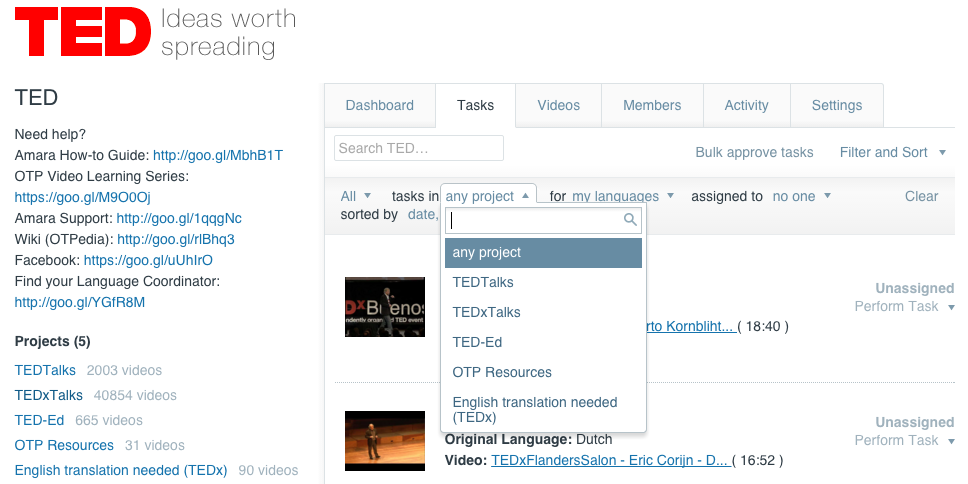
\includegraphics[width=0.7\textwidth]{textual/Figuras/TEDteamprojects.png}
        \caption{TED Teams project platform (Source: \href{https://translations.ted.com/How_to_Tackle_a_Review}{Wikipedia}).}
        \label{fig: ted-team-project}
        \end{figure}
        
    \item[TED2013:] This is a separate parallel corpus of TED Talks subtitles provided by CASMACAT\footnote{\href{http://www.casmacat.eu/corpus/ted2013.html}{http://www.casmacat.eu/corpus/ted2013.html}}, as described in~\textcite{tiedemann-2012-parallel}. The original source of the files is WIT$^3$\footnote{\href{https://wit3.fbk.eu}{https://wit3.fbk.eu}}, which stands for \emph{Web Inventory of Transcribed and Translated Talks}. WIT$^3$ is a ready-to-use version for research purposes of the multilingual transcriptions of TED Talks. The original dateset comprises a total of 346,643 segments, with approximately 5.5 million English tokens and 5.2 million Portuguese tokens. Notably, these transcripts were also translated by volunteers into various languages.
\end{description}


\section{Data Pre-processing and Compilation}

The TED Talks datasets selected for analysis were originally downloaded in TMX (Translation Memory eXchange). While TMX is a common format for storing translations, it was not directly usable for our purposes. To make the data more suitable for manipulation and further analysis, we developed a custom Python script leveraging the \texttt{Pandas}\footnote{\href{https://pandas.pydata.org}{https://pandas.pydata.org}} library. 

This script streamlines the conversion process by offering several key functionalities:

\begin{description}
    \item[DataFrame Structure:] We transformed data from TMX format into a Pandas DataFrame. This format is ideal for data manipulation, analysis, and integration with other Python libraries.
    \item[Large File Handling:] We identified and split large TMX files exceeding a user-defined size threshold into smaller chunks for efficient processing, preventing memory issues.
    \item[Metadata Preservation:] We preserved metadata from the original files by setting the \texttt{metadata=True} argument in the \texttt{clean\_data\_loader} function. This can be valuable for understanding the context and origin of the translation data.
    \item[Unique Data Point Identification:] We added an \texttt{inner\_id} column to the DataFrame, providing a unique identifier for each data point within the final CSV file. This facilitates tracking data points and merging datasets if necessary.
\end{description}

To illustrate the TMX conversion process, consider the following example from our corpus highlighting how the script transforms data from a less user-friendly XML format (TMX) into a structured and analyzable format (Pandas DataFrame):

\begin{verbatim} 
<tuv xml:lang="en">
  <seg> Put yourselves in my position. </seg>
</tuv>
<tuv xml:lang="pt">
  <seg> Coloquem-se no meu lugar! </seg>
</tuv>
\end{verbatim}


This snippet shows a portion of a TMX file containing a translation unit (TU) with two segments (seg). The first segment is in English (``Put yourselves in my position.''), and the second segment is its Portuguese translation (``Coloquem-se no meu lugar!'').

\begin{table}[htb]
\small
\centering
\begin{tabular}{|c|p{3cm}|p{3cm}|c|p{3cm}|}
\hline
\centering
{\textbf{lang\_pair}} & {\textbf{source}} & {\textbf{target}} & \textbf{inner\_id} & \textbf{produced\_from} \\ \hline\hline
en\_pt\_br & Put yourselves in my position. & Coloquem-se no meu lugar! & 4 & SRC\_TM\_DATA/ data\_2024/en-pt-2\_br.tmx \\ \hline
\end{tabular}
\caption{Example of Pandas DataFrame (after TMX conversion).}
\label{tab:example-pandas}
\end{table}

Table~\ref{tab:example-pandas} displays a portion of the resulting Pandas DataFrame after processing the TMX file. Each row represents a translation unit (TU). The DataFrame includes columns for the source sentence, target sentence, source language code, target language code, and potentially additional metadata preserved from the original file. An ``inner\_id'' column is also added for unique identification within the DataFrame.


\subsection{Data Cleaning and Normalization Steps}

This section details the data cleaning process applied to prepare the TED Talks transcript data for NMT engine training and evaluation. Following the initial conversion to a Pandas DataFrame, the cleaning steps aimed to ensure data quality and consistency for an effective analysis.

\begin{description}
    \item[Project Organization:] A well-structured project directory with subdirectories for each pre-processing stage was created to facilitate data organization and tracking throughout the cleaning pipeline.
    \item[Basic Cleaning Functions:] 
    \begin{description}
        \item[Missing Values \& Extraneous Markup Removal:] Rows containing missing entries (null values) and any residual HTML tags or code snippets were removed. Common parsers like \texttt{lxml}\footnote{\href{https://lxml.de}{https://lxml.de}}, \texttt{html.parser}\footnote{\href{https://docs.python.org/3/library/html.parser.html}{https://docs.python.org/3/library/html.parser.html}}, and \texttt{html5lib}\footnote{\href{https://pypi.org/project/html5lib/}{https://pypi.org/project/html5lib/}} were used for efficient HTML tag removal.
        \item[Duplicate Removal:] Identical entries in the dataset, potentially arising from data collection or processing errors, were removed to ensure each data point represents a unique translation pair.
        \item[Emoji Removal:] A custom function was implemented to identify and remove rows containing emojis, as they may not translate well using NMT engines.
    \end{description}
    \item[Targeted Cleaning:]
    \begin{description}
        \item[Incomplete Sentence Removal:] Sentences starting with punctuation marks in either source or target languages were removed, as they may represent incomplete phrases and hinder the translation process.
        \item[Strange Pattern Removal:] Unwanted strange text patterns were identified and removed using regular expressions (\texttt{re}\footnote{\href{https://docs.python.org/3/library/re.html}{https://docs.python.org/3/library/re.html}} library). This addressed noise or repetitive phrases that could also hinder the translation analysis.
        \item[Length Filtering:] Sentences outside a specific word and/or character range were excluded from the dataset to ensure reasonably manageable content size for NMT processing. This filtering included:
        \begin{description}
            \item \textbf{Token-based} (min: 4, max: 200): Sentences within this specific range of words/punctuation marks were retained.
            \item \textbf{Character-based} (min: 200, max: 450): Sentences within this specific range of characters (including punctuation marks) were retained.
            \item \textbf{Character-based Proportion} (lower: 0.001, upper: 0.999): Character proportions were calculated and mismatches in length between source and target texts were filtered out for better aligned translations.
        \end{description}
        \item[Repetition Removal:] Segments with excessively repetitive terms were removed, as they may not provide valuable data for the NMT engine.
        \item[Language Detection:] The \texttt{FastText}\footnote{\href{https://fasttext.cc/docs/en/python-module.html}{https://fasttext.cc/docs/en/python-module.html}} model identified languages within the data segments. Any segments in a language different from the source (English) and target (Portuguese) languages were filtered out.
        \item[Identical Text Removal:] Segments where source and target texts were exactly the same were deleted, as they do not represent actual translations.
        \item[Rare Characters Removal:] Rare characters with very low occurrence counts were identified and any segments containing them were removed to avoid introducing noise from infrequent characters (see Appendix~\ref{app:1} for examples).
        \end{description}
    \item \textbf{Extra Cleaning}:
    \begin{description}
        \item[Duplicate Removal (Recheck):] An additional check for duplicate entries was performed to ensure all duplicates were removed after the previous steps.
        \item[LaBSE Scoring:] LaBSE\footnote{\href{https://blog.research.google/2020/08/language-agnostic-bert-sentence.html}{https://blog.research.google/2020/08/language-agnostic-bert-sentence.html}} (Language-agnostic BERT Sentence Embedding), a multilingual sentence embedding model, was be used to calculate estimates of translation quality. Segments with LaBSE scores below a specific threshold were dropped to focus on higher-quality translations.
    \end{description}
    \item[Statistics Report:] A table summarizing the different types of deleted segments and their counts (from highest to lowest) was generated. This report provided insights into the cleaning process effectiveness and the quality of the original data.
\end{description}


\subsection{Refining the Dataset for NMT Testing and Evaluation}

This section details the multi-step process of filtering our data to create an optimal dataset for NMT engine evaluation, initially dividing the files into training and testing sets. However, despite a few attempts to build a custom NMT model using the Seq2Seq\footnote{\href{https://www.tensorflow.org/text/tutorials/nmt\_with\_attention}{https://www.tensorflow.org/text/tutorials/nmt\_with\_attention}} approach, our model resulted in subpar performance due to insufficient computational resources, time constraints, and the complexity of replicating the NMT task. Consequently, we decided to pursue the evaluation approach, which will be discussed in a later section.


\subsubsection{Further Refinement Steps}

To ensure the test set aligned with common translation scenarios while reflecting the focus of our research on spatial prepositions, we implemented the following filters:

\begin{description}
    \item[Sentence Segmentation:] We excluded entries containing multiple sentences, as NMT engines typically handle sentences individually.
    \item[Minimum Length:] Segments deemed too short were also removed, focusing on translations with a minimum required complexity.
    \item[Formatting:] Entries that began with a lowercase letter or lacked proper ending punctuation were also excluded to maintain consistency and well-formed structure.
    \item[Focus on Spatial Preposition:] Following our research goals of analyzing translations involving relevant spatial meanings, we prioritized sentences containing at least one of the prepositions: ACROSS, THROUGH, INTO, and ONTO.
\end{description}   

These additional filters reduced the initial dataset to a final size of $2,000$ segments, providing a more focused and effective test set for NMT engine testing and evaluation specific to spatial prepositions.

\section{Categorization by Meanings}

We employed a systematic approach to categorize prepositions in each EN source sentence based on their spatial and non-spatial meanings. This categorization is aligned with the definitions proposed by~\textcite{bruckfield2011prepositions} and entries found in the Cambridge Online Dictionary (CAM)\footnote{\href{https://dictionary.cambridge.org/}{https://dictionary.cambridge.org/}}. The specific categorizations are detailed in Table~\ref{tab:prep-categorizations}. 

\begin{table}[htb]
\small
\centering
\begin{tabular}{lp{.7\textwidth}}
\toprule
\textbf{EN Preposition} & \textbf{Meaning(s)}
\\ \midrule
Across  & \begin{tabular}[c]{@{}l@{}}(i) Perpendicular position; \\ (ii) Movement over a surface; \\ (iii) Opposite location; \\ (iv) Distribution; \\ (v) Non-spatial \end{tabular} \\
\hline
Into & \begin{tabular}[c]{@{}l@{}}(i) Movement or direction leading to enclosure; \\ (ii) Movement resulting in physical contact or collision; \\ (iii) Non-spatial \end{tabular} \\
\hline
Onto & \begin{tabular}[c]{@{}l@{}}(i) Movement to a location on a surface; \\ (ii) Sense of attachment; \\ (iii) Non-spatial \end{tabular} \\
\hline
Through & \begin{tabular}[c]{@{}l@{}}(i) Movement within a passage or conduit; \\ (ii) Movement within an open area, region, or place; \\ 
(iii) Movement past or penetrating a barrier;  \\ (iv) Part of a route; \\ (v) Non-spatial
\end{tabular} \\
\bottomrule  
\end{tabular}
\caption{Categorization of ACROSS, THROUGH, INTO, and ONTO (adpated from \textcite{bruckfield2011prepositions} and CAM).}
\label{tab:prep-categorizations}
\end{table}

Here are three examples of source sentences containing the preposition ACROSS included in this test set after the final filtering:

\ex. I woke up, they opened the door, I went out to get some fresh air, and I looked, and there was a man running \emph{across} $^{\textsuperscript{ii}}$ the runway. (\texttt{inner\_id: 30}) \label{ex: across-2}

Explanation: The superscript \emph{ii} corresponds to the specific meaning Across(ii) in Table~\ref{tab:prep-categorizations}, which refers to ``Movement over a surface.''

\ex. And so then Tarja was sitting \emph{across} $^{\textsuperscript{iii}}$ the table from me. (\texttt{inner\_id: 3011154}) \label{ex: across-3}

Explanation: The superscript \emph{iii} corresponds to the specific meaning Across(iii) in Table~\ref{tab:prep-categorizations}, which refers to ``Opposite location.''

\ex. In the mid-19th century, suspension bridges were collapsing all \emph{across} $^{\textsuperscript{iv}}$ Europe. (\texttt{inner\_id: 343660}) \label{ex: across-4}

Explanation: The superscript \emph{iv} corresponds to the specific meaning Across(iv) in Table~\ref{tab:prep-categorizations}, which refers to ``Distribution.'' 

Examples~\ref{ex: across-2}, \ref{ex: across-3} and \ref{ex: across-4} showcase the variety of contexts for ACROSS, as summarized in Table~\ref{tab:prep-categorizations}. These examples allow for a more nuanced evaluation of NMT engines' ability to capture the subtleties of spatial prepositions during translation.


\section{The Translation Process}

To ensure reproducibility, we prioritized freely available resources for translating our test set across different platforms. These resources included Python libraries, APIs, and open-source language models. However, limitations like request quotas and character restrictions necessitated the development of alternative strategies (details provided later).

\subsection{NMT Systems}

We employed three established NMT service providers for our evaluation:

\subsubsection{Google Translate}

To translate using Google Translate, we employed the \texttt{googletrans}\footnote{\href{https://pypi.org/project/googletrans/}{https://pypi.org/project/googletrans/}} a free and open-source Python library, to leverage Google Translate Ajax API. This library allows users to translate text directly within their Python code, utilizing the same servers that power translate.google.com.

\subsubsection{DeepL Translator}

Due to limitations on free access, we utilized a combination of resources for DeepL:

\begin{description}
    \item[\hspace{=2em}Rapid API]\footnote{\href{https://rapidapi.com/splintPRO/api/deepl-translator/}{https://rapidapi.com/splintPRO/api/deepl-translator/}}: This server provided programmatic access with limited requests per minute.
    \item[\hspace{=2em}DeepL Console]\footnote{\href{https://www.deepl.com/en/translator}{https://www.deepl.com/en/translator}}: Offered a web interface for manual translations, but with limitations on the number of translated tokens.
    \item[\hspace{=2em}DeepL Desktop App] (installed on a Macbook Pro Late 2013 -- see Figure~\ref{fig: deepl-app}): Facilitated offline translation capabilities, allowing us to translate larger batches.
\end{description}



For efficiency, the test set was translated in batches of 50 sentences each. All DeepL translations were then compiled into a single file for further analysis. 

\begin{figure}[htb]
\centering
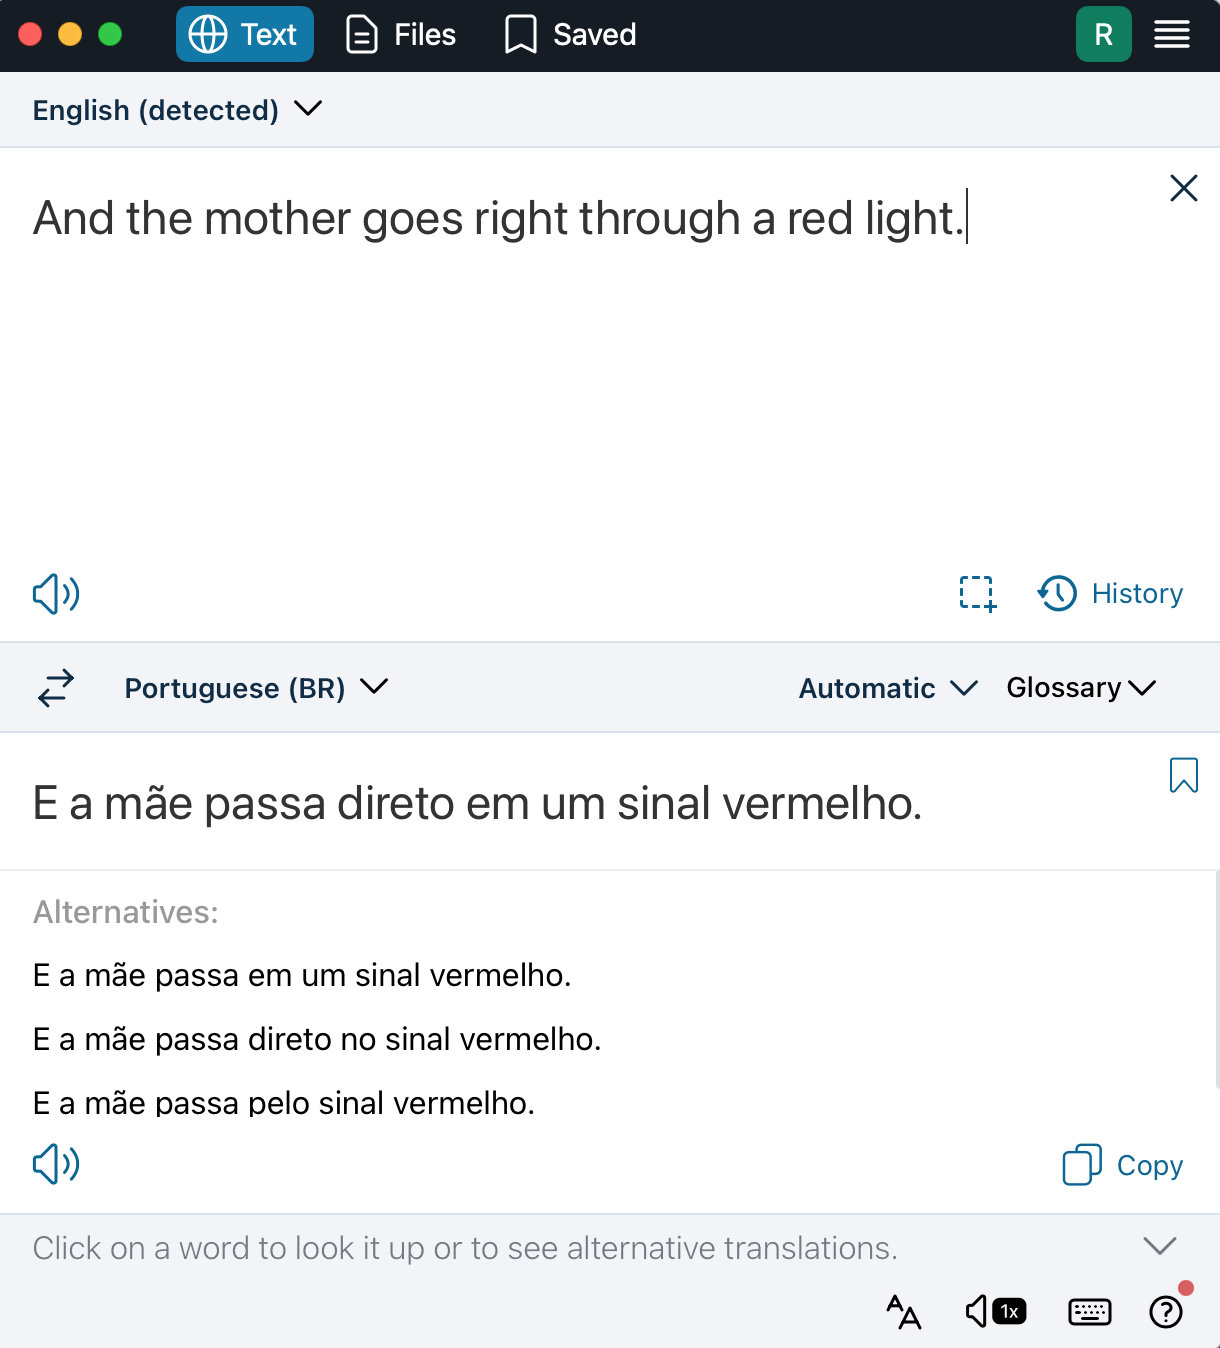
\includegraphics[width=0.6\textwidth]{textual/Figuras/deepl-app.png}
\caption{DeepL Translator app interface (Source: Our own).}
\label{fig: deepl-app}
\end{figure}

\subsubsection{Amazon Translate}

We utilized Amazon's  console\footnote{\href{https://console.aws.amazon.com/translate/home}{https://console.aws.amazon.com/translate/home}} and a free AWS account for the translation taks.

\begin{description}
    \item[\hspace{=2em}Amazon (Stock):] We leveraged the free Batch translation service to translate the 2,000-segment test set from a single CSV file.
    \item[\hspace{=2em}Amazon (Custom):] We trained a custom model using the parallel data option on Amazon Translate with the remaining 344,643 segments from the training set. This allowed us to explore the impact of model customization on translation quality.
\end{description}


\subsection{LLMs}

To perform machine translations using LLMs, we utilized the Python library \texttt{Ollama} \footnote{\href{https://github.com/ollama/ollama-python}{https://github.com/ollama/ollama-python}}, which facilitates running open-source generative models locally or on the cloud through \texttt{LangChain}\footnote{\href{https://api.python.langchain.com/en/latest/community_api_reference.html}{https://api.python.langchain.com/en/latest/community\_api\_reference.html}}. This allowed us to explore the capabilities of LLMs for translation tasks. However, it is important to note that the computational demands of LLMs required the use of Google Colab Pro with its enhanced GPUs for efficient processing.

\subsubsection{Meta's LLaMa}

We experimented with three variations of the  open-source LLaMa family:

\begin{description}
\item[\hspace{=2em}LLaMa 3 (8B)]\footnote{\href{https://huggingface.co/meta-llama/Meta-Llama-3-8B}{https://huggingface.co/meta-llama/Meta-Llama-3-8B}}: As of the date of this work, this is the latest generation of LLaMa. It adopts a decoder-only transformer architecture and employs a tokenizer with a vocabulary of 128K tokens, facilitating more efficient language encoding. Throughout training, the model processes sequences of 8,192 tokens while utilizing a mask to prevent self-attention from extending beyond document boundaries. Trained on a dataset of 15 trillion tokens, it stands as the most advanced LLaMa model to date, featuring an 8K context length—twice that of LLaMa 2. This significant advancement is reinforced by over 5\% non-English pretraining data, covering more than 30 languages~\parencite{llama3}.    \item[\hspace{=2em}LLaMa 2 Uncensored]\footnote{\href{https://huggingface.co/georgesung/llama2_7b_chat_uncensored}{https://huggingface.co/georgesung/llama2\_7b\_chat\_uncensored}}: This uncensored version, developed by George Sung and Jarrad Hope and based on Meta's open-source Llama 2, underwent training on 2 trillion tokens. With 7 billion parameters and a size of 3.8GB, this model was pretrained on publicly available online data sources. Its architecture follows the decoder-only variant of transformers and employs a tokenizer with a vocabulary of 128K tokens, which is 40\% larger than LLaMa 1. Notably, this model offers unrestricted outputs, distinguishing it from the original Llama 2 and making it suitable for various applications \parencite{llama2}.
    \item[\hspace{=2em}LLaMa 2 (13B)]\footnote{\href{https://huggingface.co/meta-llama/Llama-2-13b}{https://huggingface.co/meta-llama/Llama-2-13b}}: The 13B Llama 2 boasts a larger size (13B parameters) compared to the 7B version. This increase suggests potential for capturing more complex language patterns, which could lead to potentially improved performance in various tasks. Both models likely utilize the same decoder-only transformer architecture, excelling at text generation. However, information on the 13B's output limitations is currently unavailable. Further testing  is needed to definitively determine any performance advantage the 13B model holds over the 7B version \parencite{llama2}.
\end{description}

 
\subsubsection{Google's Gemma}

We examined Gemma 7B \parencite{gemma_2024, gemma}, a lightweight open-source language model from Google, built using technology similar to Gemini models. It is a text-to-text, decoder-only large language models, available in English, possessing open weights, pre-trained variants, and instruction-tuned variants. It was trained on a dataset of 6 trillion tokens and a context length of 8192 tokens. The specific composition of this data is not publicly available. Gemma excells in tasks such as text generation, question answering, summarization, and reasoning, and can be fine-tuned for other tasks.


\subsubsection{Mistral Models}

We also investigated two open-source models by Mistral AI:

\begin{description}
    \item[\hspace{=2em}Mixtral-8x7B (47B)]\footnote{\href{https://huggingface.co/mistralai/Mixtral-8x7B-v0.1}{https://huggingface.co/mistralai/Mixtral-8x7B-v0.1}}: Mixtral, a decoder-only language model, leverages a sparse mixture-of-experts network for cost-efficiency. Trained on publicly available web data \parencite{mixtral}, Mixtral employs a similar architecture to Mistral 7B, but with each layer utilizing 8 expert blocks. This approach allows access to a larger parameter pool (47 billion) while actively using only a portion (13 billion) during inference, leading to cost savings. Additionally, Mixtral boasts a large context window (32k tokens) and native multilingual capabilities (English, French, German, Spanish, Italian). This combination positions Mixtral as a strong contender for various NLP tasks \parencite{jiang2024mixtral}.
    \item[\hspace{=2em}Mistral (7B) Instruct v0.2]\footnote{\href{https://huggingface.co/mistralai/Mistral-7B-Instruct-v0.2}{https://huggingface.co/mistralai/Mistral-7B-Instruct-v0.2}}: Mistral 7B is a decoder-only 7-billion parameter, open-source language model (LLM) achieving competitive performance on various benchmarks \parencite{mistral, jiang2023mistral}. It employs grouped-query attention (GQA) and sliding window attention (SWA) for efficient text processing, particularly for handling long sequences. Mistral 7B's adaptability allows it to generate responses based on instructions and predict missing text, making it suitable for tasks like chatbots and content generation.
    \end{description}

To collect the translations, two zero-shot prompt variations were used:

\newtcolorbox{promptbox}{
colback=gray!5,
arc=4pt,
left skip=5pt,
right skip=5pt,
boxsep=5pt,
fonttitle=\bfseries,
boxrule = 0pt,
toprule = 4.5pt,
enhanced,
fuzzy shadow = {0pt}{-2pt}{-0.5pt}{0.5pt}{black!35},
width=\textwidth,
title=Standard Prompt:
}

\begin{promptbox}
context  $=$ ``You are a professional translator.'' \\
task $=$ ``Translate the following sentence from English to Portuguese: \textbf{[source\_text]}'' 
\end{promptbox}

\newtcolorbox{promptbox1}{
colback=gray!5,
arc=4pt,
left skip=5pt,
right skip=5pt,
boxsep=5pt,
fonttitle=\bfseries,
boxrule = 0pt,
toprule = 4.5pt,
enhanced,
fuzzy shadow = {0pt}{-2pt}{-0.5pt}{0.5pt}{black!35},
width=\textwidth,
title=Alternative Prompt:
}

\begin{promptbox1}
context  $=$ ``You are a professional translator.'' \\
task $=$ ``Translate the following sentence from English to Portuguese: \textbf{[source\_text]}. Provide only ONE translation. DON'T add any additional comments, observations or translations.''
\end{promptbox1}


\section{The Scoring Step}

This section details the subsequent scoring process for translation quality evaluation, after data collection and post-editing. We utilized Python libraries to calculate these scores for each data point.


\begin{description}
    \item[NLTK:] Both BLEU and METEOR scores were calculated using the \texttt{nltk}\footnote{\href{https://www.nltk.org}{https://www.nltk.orgl}} library, which handles text tokenization (splitting sentences into words) as a pre-processing step. The \texttt{nltk.translate} submodule provides functions for calculating:
    \begin{description}
        \item[BLEU score:] \texttt{bleu\_score}\footnote{\href{https://www.nltk.org/api/nltk.translate.bleu_score.html}{https://www.nltk.org/api/nltk.translate.bleu\_score.html}} with \texttt{SmoothingFunction().method1} focuses on \emph{n}-gram (sequence of \emph{n} words) overlaps between the reference and translated text, with adjustments for cases with missing values in the translation.
        \item[METEOR score:] \texttt{meteor\_score}\footnote{\href{https://www.nltk.org/api/nltk.translate.meteor_score.html}{https://www.nltk.org/api/nltk.translate.meteor\_score.html}} considers factors like unigram precision, recall, synonym matching, and stemming to assess translation quality. 
    \end{description}
    \item[SacreBLEU:] TER scores were calculated using the \texttt{sentence\_ter} function from the  \texttt{sacrebleu}\footnote{\href{https://github.com/mjpost/sacrebleu/tree/master}{https://github.com/mjpost/sacrebleu/tree/master}} library. It measures the number of edits (insertions, deletions, substitutions) required to transform the translated text into the reference text.
    \item[Transformers:] We calculated BERTScores to assess semantic similarity between reference and translated texts utilizing the \texttt{transformers} library to load a pre-trained BERT model and tokenizer\footnote{\href{https://huggingface.co/transformers/v3.0.2/model_doc/bert.html}{https://huggingface.co/transformers/v3.0.2/model\_doc/bert.html}}. BERT works by generating sentence embeddings, which capture the meaning of a sentence in a high-dimensional space. We calculate the cosine similarity between these embeddings to determine how close the semantics of the reference and translated text are.
    \item[Cometml:] The \texttt{cometml}\footnote{\href{https://pypi.org/project/comet-ml/}{https://pypi.org/project/comet-ml/}} library was used to load the pre-trained COMET model named ``Unbabel/wmt22-comet-da''. This model is specifically designed for evaluating translation quality, focusing on aspects like fluency, adequacy, and coherence. We formatted our data to match the model's input requirements and then retrieved the score based on the model's prediction.
\end{description}


\section{Score Distributions and Confidence Intervals}

To analyze the distribution of scores across models, box plots were utilized, offering a visual summary of the data's key statistics: minimum, first quartile (Q1), median, third quartile (Q3), and maximum. Additionally, confidence intervals (CIs) were computed at a 95\% confidence level to estimate the likely range of the true difference between the means of compared systems, based on the calculated means \parencite{zhang-vogel-2004-measuring}. This approach facilitated an understanding of the precision among models and statistical significance. Refer to Figures \ref{fig:boxplot} and \ref{fig:ci} for visual representations of these steps.

For these analyses, the following Python libraries for statistical computations were employed: \texttt{NumPy}\footnote{\href{https://numpy.org}{https://numpy.org}} for numerical operations, including functions for median, quartiles, percentiles, mean, and standard deviation; and \texttt{SciPy}\footnote{\href{https://scipy.org}{https://scipy.org}} for statistical functions such as \texttt{stats.t.interval} to calculate CIs.

\begin{figure}[htb]
\centering
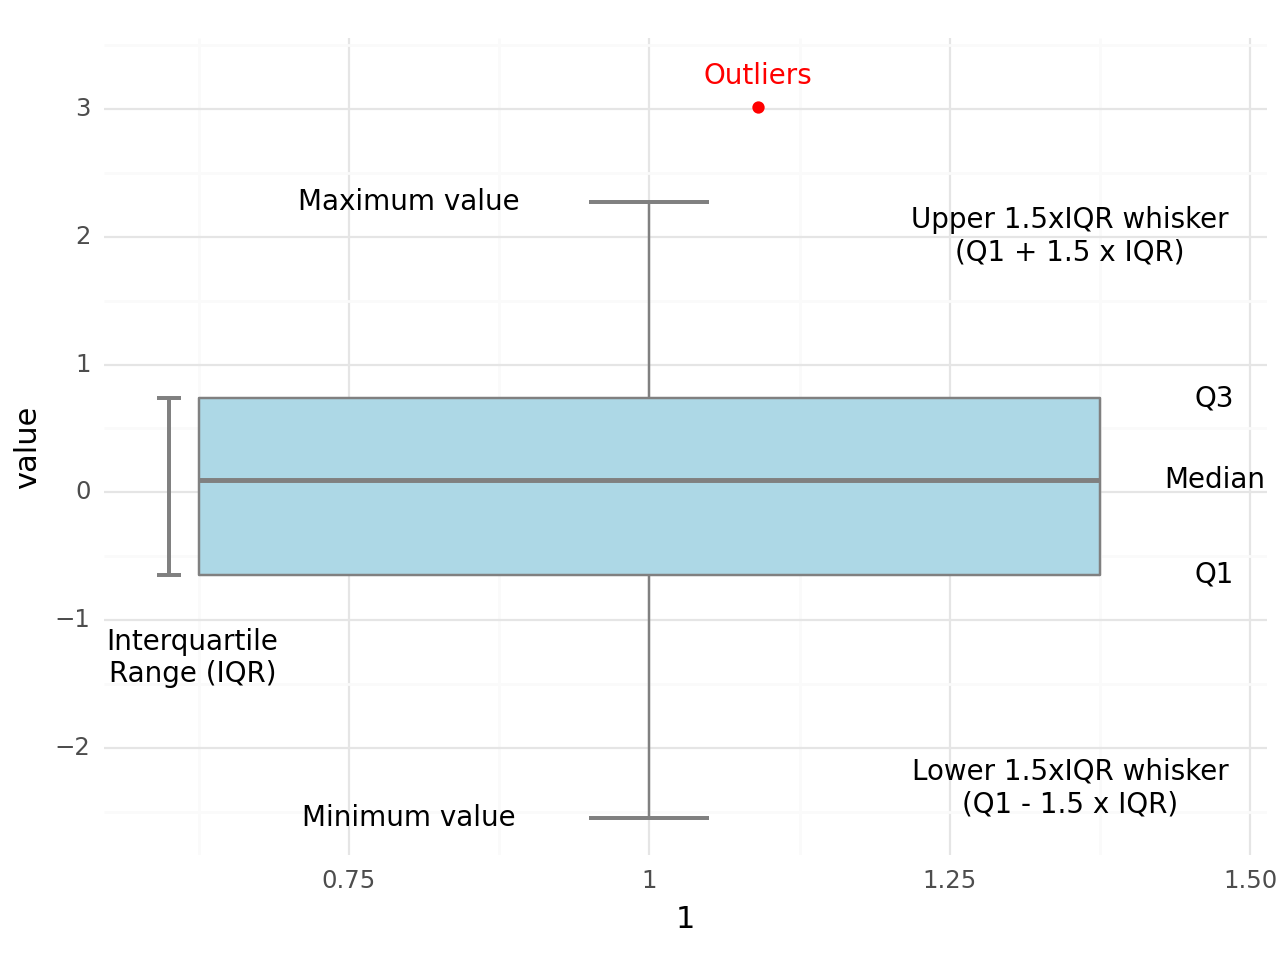
\includegraphics[width=.8\textwidth]{textual/Figuras/boxplot-real.png}
\caption{Key Features of Box Plot (Source: Our own).}
\label{fig:boxplot}
\end{figure}

Key features of the boxplot:

\begin{description}
    \item[Minimum Value:] The lowest score, excluding outliers (shown at the end of the bottom whisker).
    \item[Lower Quartile:] Twenty-five percent of scores fall below the lower quartile value (also known as the first quartile).
    \item[Median:] The median marks the mid-point of the data and is shown by the line that divides the box into two parts (sometimes known as the second quartile). Half the scores are greater than or equal to this value, and half are less.
    \item[Upper Quartile:] Seventy-five percent of the scores fall below the upper quartile value (also known as the third quartile). Thus, 25\% of data are above this value.
    \item[Maximum Value:] The highest score, excluding outliers (shown at the end of the top whisker).
    \item[Whiskers:] The upper and lower whiskers represent scores outside the middle 50\% (i.e., the lower 25\% of scores and the upper 25\% of scores).
    \item[Interquartile Range (IQR):] The box plot shows the middle 50\% of scores (i.e., the range between the 25th and 75th percentile).
    \item[Outliers:] Individual data points that fall outside the whiskers and are typically considered as extreme values.
\end{description}

The quartiles (Q1 and Q3) and the interquartile range (IQR) were calculated using the \texttt{np.percentile} function from \texttt{NumPy}. The whiskers were then determined by extending from the quartiles by 1.5 times the IQR, ensuring that they include the most extreme non-outlier data points within that range.

\begin{figure}[htb]
\centering
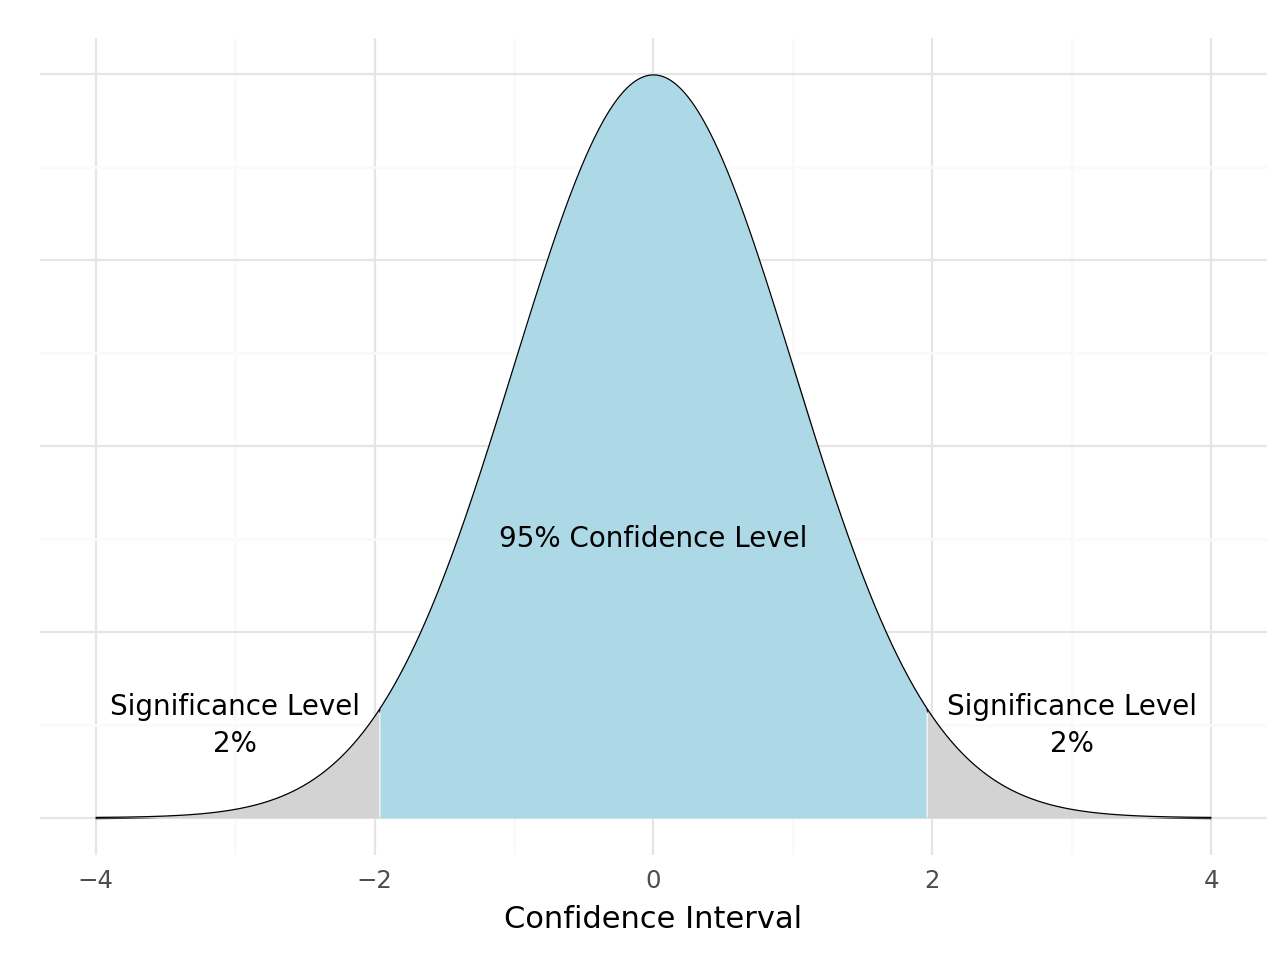
\includegraphics[width=.6\textwidth]{textual/Figuras/confidence-intervals.png}
\caption{Confidence Intervals (CIs) (Source: Our own).}
\label{fig:ci}
\end{figure}


To calculate CIs, we used the \texttt{stats.t.interval} function from the \texttt{scipy.stats} module. This function employs the Student’s t-distribution to compute the interval for a specified confidence level. The probability density function (pdf) is given by:

\begin{equation} \label{formula: t-dis}
f(x|df) = \frac{\Gamma\left(\frac{df+1}{2}\right)}{\sqrt{\pi df} \, \Gamma\left(\frac{df}{2}\right)} \left(1 + \frac{x^2}{df} \right)^{-\frac{df+1}{2}}
\end{equation} 

where $x$ is a real number, $df$ represents the degrees of freedom parameter and $\Gamma$ is the gamma function \parencite{scipy_stats_t}. The parameters utilized in this function include:

\begin{description}
    \item[Confidence Level (0.95):] Specifies the probability that the calculated interval contains the true population parameter, typically set to 95\%.
    \item[Degrees of Freedom:] Determined by the sample size, calculated as the number of observations minus one.
    \item[Location Parameter] (\texttt{mean\_score}): Represents the mean of the distribution, serving as the center around which the interval is constructed.
    \item[Scale Parameter] (\texttt{stats.sem(filtered\_scores)}): Estimates the standard deviation of the sample mean, used to scale the interval width.
\end{description}


After specifying these parameters, the \texttt{stats.t.interval} function computes the CI and returns the lower and upper bounds of the interval.

\section{Human Evaluation Process}
\label{sec: Human Evaluation}

This section outlines the systematic approach used to evaluate translation quality using human reviews and manual error classification. The goal was to accurately assess model performance and ultimately identify areas for improvement in translation quality.

At this stage, it is worth noting that not all models from the previous step were selected for manual analysis. Instead, we focused on comparing LLM performace against traditional NMT systems. To this end, we conducted a comprehensive analysis of all LLMs, comparing them against each other and against the top NMT performer from the scoring stage. This comparison aimed to validate the accuracy of the scores and confirm whether there was real statistical significance in performance between the two groups.

\subsection{Data Reduction for Human Review}
To gain a deeper understanding of translation quality, we employed a two-step process to select a representative sample for human reviews:

\begin{description}
\item[Random Selection:] We initially selected a reduced representative sample comprising 200 segments (10\% of the total 2,000 translated segments) for human evaluation. This process was designed to ensure randomness and diversity within the sample. We shuffled 500 segments using the Pandas' \texttt{sample}\footnote{\href{https://pandas.pydata.org/pandas-docs/stable/reference/api/pandas.DataFrame.sample.html}{https://pandas.pydata.org/pandas-docs/stable/reference/api/pandas.DataFrame.sample.html}} function.
\item[Subset Curation:] From the initially shuffled pool, human judgment was employed to review the segments and curate a refined subset of 200 segments to undergo human reviews. This approach ensured a sufficient sample size encapsulating a variety of errors for thorough analysis.
\end{description}


\subsection{Manual Error Classification}
\label{subsec: Manual Error Classification}

In this step, each translated segment underwent a meticulous manual error classification process to identify and categorize translation errors accurately, comprehensively, and efficiently. The error classification scheme, organized into two main categories, is detailed in Table~\ref{tab: error_categories}. This scheme was utilized to systematically identify and categorize errors, enabling a more precise, nuanced, and reliable assessment of model performance.

\begin{table}[htb]
\centering
\small
\begin{tabular}{lp{.5\textwidth}}
\toprule
\textbf{Annotations} & \textbf{Description} \\
\midrule
\quad Correct (cc) & Accurate translation. \\
\midrule
\quad \textbf{Spatial Errors} & \\
\quad \quad Polysemy (po) & Incorrect polysemous prepositional sense. \\
\quad \quad Syntactic Projection (sp) & Incorrect copy of source language syntax.  \\
\quad \quad Wrong Sense (ws) & Incorrect unrelated prepositional sense. \\
\midrule
\quad \textbf{Non-Spatial Errors} &  \\
\quad \quad Idiomatic Expression (ie) & Mistranslation of phrasal verbs or idioms. \\
\midrule
\quad \textbf{Other Errors} &  \\
\quad \quad Addition (ad) & Unnecessary added words/phrases.  \\
\quad \quad Agreement (ag) & Wrong subject-verb/noun combinations.  \\
\quad \quad Anglicism (ag) & Directly borrowed English structure.  \\
\quad \quad Collocation (co) & Incorrect verb combinations.  \\
\quad \quad Grammar/orthography (gr) &  Grammar/spelling errors.  \\
\quad \quad Interlanguage/code-switching (in) & Mixed use of target and/or other languages.  \\
\quad \quad Omission (om) & Missing words/phrases from source text.\\
\quad \quad Untranslated (un) & Source text not (fully or partly) translated. \\
\quad \quad Wrong Lexical Choice (wl) & Inappropriate noun choice. \\
\quad \quad Wrong Verb Mood/Tense (wt) & Incorrect verb mood/tense. \\
\bottomrule
\end{tabular}
\caption{Error Annotation Scheme.}
\label{tab: error_categories}
\end{table}


During the manual error classification step, each automatic translation was analyzed primarily focusing on fluency in the target language, paying occasional attention to the reference and source texts for specific types of errors. This approach facilitated an evaluation centered on the quality of the system itself and its generated output. Error types were then annotated in an additional column in the dataset for individual records.

Given that mistranslation is a broad category, in this research, we are particularly
interested in identifying four specific mistranslation errors involving prepositions:

\begin{description}
    \item[Polysemy:] These errors happen when the MT system picks the wrong meaning 
    for a polysemous preposition (with multiple 
    meanings, spatial or not). Prepositions can be tricky because their meaning depends on the context. In spatial semantics, an MT system might misinterpret the 
    meaning of a preposition in the source language, leading to an inaccurate expression in the target language. An example is translating ``a barricade across the door'' to ``uma barreira do outro lado da porta'' (on the other side of the door) in PT-br instead of ``uma barricada atravessada na porta.'' ``Atravessada'' (crossing) is more fitting in this context.
    
    \item[Syntactic Projection:] Typically an extension of polysemy, these errors occur when the MT system not only mistranslates the preposition's meaning but also directly copies the syntax (word order) from the source language to the target language. This violates the target language's rules for expressing spatial relationships, creating problems because languages express spatial relationships differently~\parencite{talmy2000toward, talmy2000towardb, slobin2005relating}. For example, the EN phrase ``to swim across the river'' (using a Manner verb and a Path preposition) requires a different grammatical construction in PT-br, such as ``atravessar o rio nadando'' (literally ``to cross the river by swimming''). A common mistranslation of this sort would be to translate the phrase as ``nadar do outro lado do rio'', as illustrated in~\textcite{fernandes-etal-2024-spatial}. 
    
    \item[Wrong Sense Errors:] These errors occur when a spatial preposition is mistranslated into a grammatically correct but semantically %M: incorrect
    incorrect
    preposition in the target language. This mismatch arises because the chosen preposition does not accurately convey any of the possible spatial meanings of the original polysemous preposition in case. For instance, translating ``The store across the street'' as ``A loja através da rua'' in PT-br results in a wrong sense error. While ``através'' can mean ``through,'' it does not correctly convey the idea of an opposite location, which ``do outro lado da rua'' (on the other side of the street) would accurately express.
    
    \item[Idiomatic Expressions:] The only non-spatial errors on the list, these typically occur when translating idiomatic phrases whose figurative meaning goes beyond the literal meaning of the individual words. Often, these expressions involve verbs and spatial prepositions, but their meaning is not necessarily spatial -- a key distinction from syntactic projection errors. For instance, translating ``to run through a list'' literally as ``correr pela lista'' (PT-br) would be a mistake. This focuses on the individual words (run + through) rather than the intended meaning, conveyed more accurately by ``ler rapidamente'' (to read quickly).
\end{description}

By employing this well-defined human evaluation process and error classification scheme, we were able to effectively assess the quality of the automatic translations and identify areas for model improvements. This comprehensive approach allowed us to compare the performance of LLMs against traditional NMT providers and confirm any statistically significant differences.


\subsection{Chi-Square Test} 
\label{sec: chi-test}

The Chi-Square ($\chi^2$) Test of Independence is a statistical method utilized to determine the association between two categorical variables. In this study, the Chi-Square test was employed using data from the human review step to validate the null hypothesis concerning the impact of spatial and non-spatial errors on the translations. The test was conducted in Python using the \texttt{chi2\_contingency}\footnote{\href{https://docs.scipy.org/doc/scipy/reference/generated/scipy.stats.chi2\_contingency.html}{https://docs.scipy.org/doc/scipy/reference/generated/scipy.stats.chi2\_contingency.html}} function from the \texttt{scipy.stats} module. Figure~\ref{fig:chi} illustrates the Chi-Square Distribution while Equation~\ref{chi-test} describes the Chi-Square test formula. The Chi-Square Test requires:

\begin{figure}[htb]
\centering
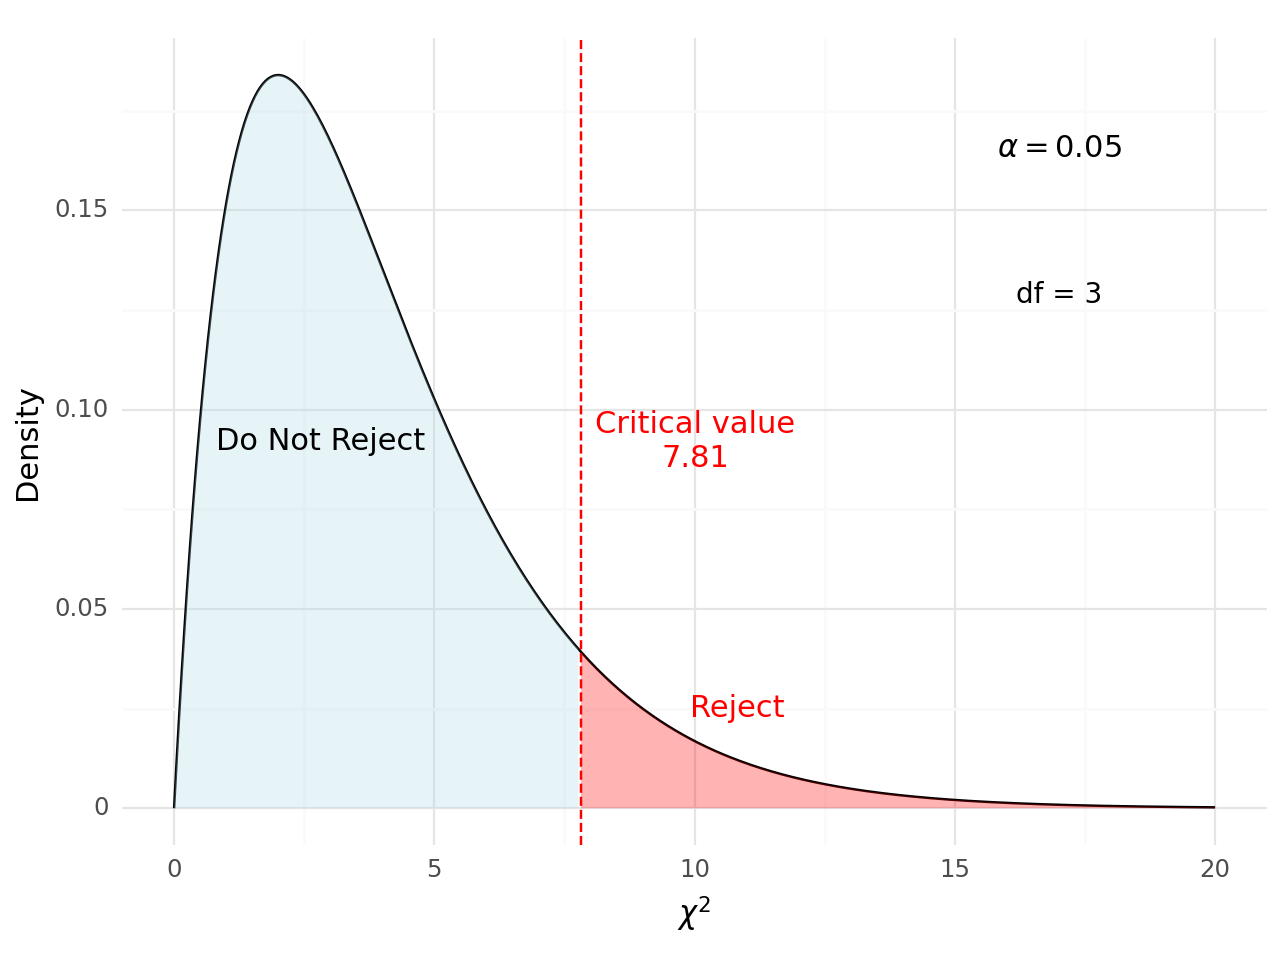
\includegraphics[width=.6\textwidth]{textual/Figuras/Results/chi.png}
\caption{Chi-Square ($\chi^2$) Distribution for $\alpha = 0.05$ and $df = 3$. (Source: Our own).}
\label{fig:chi}
\end{figure}


\begin{description}
    \item[Degrees of Freedom (df):] Depends on the number of categories or groups compared. Calculated as the number of observations minus one.
    \item[Significance Level ($\alpha$):] The probability of rejecting the null hypothesis when it is true, commonly set at $0.05$ (5\%).
    \item[Chi-Square Distribution:] Used to assess the goodness-of-fit or independence between categorical variables by comparing observed and expected frequencies.
    \item[Critical Value:] The threshold beyond which we reject the null hypothesis. For $df = 3$ and $\alpha = 0.05$, the critical value is $7.81$, obtained from chi-square distribution tables or statistical software.
    \item[\hspace{=2em}]Interpretation of the Critical Value:
    \begin{itemize}
    \item \textbf{$\chi^2 < 7.81$:} Fail to reject the null hypothesis. This indicates insufficient evidence to suggest a significant difference between observed and expected frequencies, implying that the observed data fits the expected distribution well.
    \item \textbf{$\chi^2 \ge 7.81$:} Reject the null hypothesis. This suggests a significant difference between observed and expected frequencies, indicating that the observed data does not fit the expected distribution well, thereby suggesting a possible relationship or effect.
\end{itemize}

\begin{equation} \label{chi-test}
    \chi^2_c = \sum \frac{(O_i - E_i)^2}{E_i}
\end{equation}

\hspace{=2em}In this formula, $c$ represents the degrees of freedom, and $O_i$ and $E_i$ are the observed and expected frequencies, respectively. If the calculated $\chi^2$ exceeds the critical value, the null hypothesis is rejected, indicating a significant difference between the observed and expected frequencies at the $0.05$ significance level.
\end{description}





The \texttt{chi2\_contingency} function from the \texttt{scipy.stats} module includes the following parameters and return values:

\begin{description}
    \item[Parameters] 
\end{description}
  
    \begin{itemize}
        \item \textbf{\texttt{observed} (array\_like):} The contingency table containing the observed frequencies (i.e., number of occurrences) in each category. In the two-dimensional case, the table is often described as an “R x C table”.
        \item \textbf{\texttt{correction} (bool, optional):} If \texttt{True}, and the degrees of freedom is 1, apply Yates’ correction for continuity. The effect of the correction is to adjust each observed value by 0.5 towards the corresponding expected value.
        \item \textbf{\texttt{lambda\_} (float or str, optional):} By default, the statistic computed in this test is Pearson’s chi-squared statistic. \texttt{lambda\_} allows a statistic from the Cressie-Read power divergence family to be used instead. See \texttt{scipy.stats.power\_divergence}\footnote{\href{https://docs.scipy.org/doc/scipy/reference/generated/scipy.stats.power\_divergence.html}{https://docs.scipy.org/doc/scipy/reference/generated/scipy.stats.chi2\_contingency.html}} for details. 
    \end{itemize}
    
\begin{description}
    \item[Returns] 
\end{description}  

    \begin{itemize}
        \item \textbf{\texttt{res} (Chi2ContingencyResult):} An object containing the following attributes:
        \begin{itemize}
            \item \textbf{\texttt{statistic} (float):} The test statistic.
            \item \textbf{\texttt{pvalue} (float):} The p-value of the test.
            \item \textbf{\texttt{dof} (int):} The degrees of freedom.
            \item \textbf{\texttt{expected\_freq} (ndarray):} The expected frequencies, based on the marginal sums of the table.
        \end{itemize}       
    \end{itemize}

\vspace{0.5em} % Adjust the value (e.g., 1em) to increase or decrease the gap

In Chapter~\ref{cap:Methods}, we outlined the methodology employed to explore spatial semantics in translation, comparing NMT systems and LLMs. These methods ensure a rigorous analysis of translation quality, focusing on the intricacies of spatial language. By establishing a robust framework for data collection and evaluation, this chapter lays a strong foundation for the subsequent discussion of results and their implications in MT studies.



    \chapter{Results and Discussion}
\label{cap:Resultados}

This chapter introduces the key findings of this research, beginning with the primary data cleaning and normalization process, which significantly refined the dataset. It analyzes translation quality in open-source LLMs compared to traditional NMT systems for prepositions ACROSS, THROUGH, INTO, and ONTO, categorizing errors and assessing proportions. Additionally, the chapter presents score distribution results for metrics BLUE, METEOR, BERTScore, COMET, and TER, evaluates model performance, and tests the impact of spatial semantics on translation quality. 


\section{Primary Data Cleaning Results}

%M: Antes de apresentar números, lembre aqui rapidamente o que foi feito
%OK
After an extensive data cleaning process involving removal of missing values, duplicates, emojis, incomplete sentences, strange patterns, and rare characters, along with techniques such as length filtering, language detection, and scoring for translation quality, a refined dataset was achieved for NMT translation and evaluation, with a specific focus on spatial prepositions. This refinement significantly enhanced data quality and homogeneity, reducing the initial $610,351$ segments from OPUS datasets to a final dataset of $346,643$ segments, representing a $43\%$ reduction. Table~\ref{tab:cleaning_reasons} outlines the top 10 reasons for segment removal during the cleaning and normalization steps. For the complete breakdown of reasons for segment removal, please refer to Appendix~\ref{app:1} at the end of this document.

\begin{table}[htb]
\centering
\begin{tabular}{lr}
\toprule
\textbf{Reason} & \textbf{Segments} \\
\midrule
Duplicate(s) & $218,427$ \\
Harmful element ``--'' in source or target & $19,343$ \\
Length in tokens is lower than the boundary (4) in source & $7,516$ \\
MTQE score is lower than 0.6 & $5,606$ \\
Length in tokens is lower than the boundary (4) in target & $4,077$ \\
Detected language is not [`pt'] (target) & $2,722$ \\
Harmful element ``['' in source or target & $1,623$ \\ 
Length in characters is higher than the boundary (450) in source & $970$ \\
Possible mismatch (beta) & $716$ \\
Rare character \$ in source or target & $254$ \\
\bottomrule
\end{tabular}
\caption{Reasons for Segment Removal During Data Cleaning.}
\label{tab:cleaning_reasons}
\end{table}

As can be seen in Table~\ref{tab:cleaning_reasons}, the data cleaning process removed a substantial number of segments. Duplicates (duplicated segments) in the corpus constituted the most frequent reason for removal, accounting for a significant portion ($218,427$ segments). Next, segments containing the harmful element ``--'' in either source or target language were removed ($19,343$ segments). This highlights the importance of identifying and eliminating redundant entries and special characters to ensure a unique and representative dataset.

The next two most common reasons for removal were related to sentence length and quality. Segments with a token count (number of words or punctuation marks) less than $4$ in either source or target languages were excluded ($7,516$ and $4,077$ segments, respectively). Additionally, segments with an MTQE score (Machine Translation Quality Estimation score) below $0.6$ were also removed ($5,606$ segments) from the dataset. A lower MTQE score suggests a lower predicted quality of translation, and filtering out these segments helps focus the analysis on higher-quality translations.

Lastly, the remaining entries in Table~\ref{tab:cleaning_reasons} detail the removal of segments for reasons such as length in characters being higher than 450, potential mismatches between source and target lengths, and character `\$' rarity ($970$, $716$, and $254$ segments, respectively).


\section{Score Distribution Results}
\label{sec:Distribution}

In this section, we present the results concerning the distribution of scores across models for the five metrics employed: BLEU, METEOR, BERTScore, COMET, and TER. Analyzing the spread of scores offers valuable insights into performance variation among models. We explore the means, medians, standard deviations, quartile values (Q1 and Q3), delineate the range covered by the whiskers, and compute confidence intervals to achieve a broad understanding of the data distribution and statistical significance among models.


\subsection{BLEU Across Models}

Figure~\ref{fig: blue-models} utilizes BLEU scores to assess model performance. BLEU measures similarity between a generated text and a reference translation by considering \emph{n-}gram precision (how often word sequences match) and a brevity penalty (to avoid overly short outputs). This simple and widely used metric, along with other statistical measures, provides valuable insights into the quality of the text generated by the models.

\begin{figure}[htb]
        \centering        \includegraphics[width=.9\textwidth]{textual/Figuras/Results/unknown-37.png}
        \caption{Distribution of BLEU Across Models..}
        \label{fig: blue-models}
\end{figure}


\subsubsection{Mean and Median}

When comparing the mean (depicted by red circles) and median scores (represented by black lines) in models like Amazon, DeepL, Google, and Mixtral-8x7B, they generally align closely, indicating symmetrical distributions. However, slight differences between means and medians in some LLMs suggest potential effects of outliers in their distributions. Analyzing medians in relation to quartiles offers insights into data spread and model characteristics. For instance, all models consistenly show medians closer to the upper quartile, suggesting that a significant portion of their data falls within higher score ranges.


\subsubsection{Spread of Data}

The interquartile range (IQR), i.e. the difference between the third quartile (Q3) and the first quartile (Q1), serves as a measure of data spread. Models with wider IQRs, such as Amazon, DeepL, and Google, as well as others like Mixtral-8x7B and LLaMa-3-8B, exhibit greater variability compared to those with narrower IQRs, like Mistral-7B, LLaMa-2-7B, and Gemma-7B. Across all models, the lowest whisker is observed close to zero, indicating their lower range, while Amazon (Custom) boasts the highest whisker, nearing $0.942$, indicative of its higher range. Among LLMs, Mixtral-8x7B, LLaMa-3-8B, and LLaMa-2-13B demonstrate wider IQRs, suggesting slightly more variability, whereas LLaMa-2-7B and Gemma-7B exhibit narrower IQRs, indicating more consistent lower performance.


\subsubsection{Outliers}

The presence of outliers, indicated by values beyond the boxplot whiskers (black dots), signifies notable deviations in performance among specific models compared to the dataset. These outliers may represent either exceptionally high or low performance relative to the majority of data points. Specifically, outliers positioned above the upper whisker denote exceptionally high data points, suggesting performance that stands out from the dataset's norm. Among LLMs, models like Gemma-7B and LLaMa-2-7B display the lowest upper-position outliers, implying less variability in their top performance compared to others.


\subsubsection{Confidence Intervals}

The analysis of confidence intervals (CIs) in Table~\ref{tab:mean_ci_scores_blue} provides insights into the precision of mean BLUE score estimates for different models. Models like Google, Gemma-7B, LLaMA-2-7B, LLaMA-2-13B, LLaMA-3-8B, and Mixtral-8x7B have CIs that do not overlap with each other, suggesting potential significant differences in their mean BLUE scores and statistical significance. Conversely, models like Amazon (Custom), Amazon (Stock), and DeepL exhibit overlapping intervals, implying their mean BLUE scores may not be statistically different.

\begin{table}[htb]
\centering
\begin{tabular}{lccc}
\toprule
\textbf{Model} & \textbf{Mean} & \textbf{CIs} & \textbf{SD} \\
\midrule
Amazon (Custom) & $0.370$ & [$0.361$, $0.379$] & $0.1998$ \\
Amazon (Stock) & $\mathbf{0.375}$ & [$0.366$, $0.383$] & $0.1915$ \\
DeepL & $0.366$ & [$0.358$, $0.374$] & $0.1905$ \\
Gemma-7B & $0.011$ & [$0.010$, $0.011$] & $0.0045$ \\
Google & $0.335$ & [$0.327$, $0.343$] & $0.1827$ \\
LLaMA-2-13B & $0.233$ & [$0.226$, $0.240$] & $0.1623$ \\
LLaMA-2-7B & $0.169$ & [$0.163$, $0.175$] & $0.1337$ \\
LLaMA-3-8B & $0.264$ & [$0.257$, $0.271$] & $0.1656$ \\
Mistral-7B & $0.207$ & [$0.200$, $0.213$] & $0.1477$ \\
Mixtral-8x7B & $0.273$ & [$0.266$, $0.280$] & $0.1664$ \\
\bottomrule
\end{tabular}
\caption{Means, Confidence Intervals (CIs), and Standard Deviations (SD) for BLUE scores.}
\label{tab:mean_ci_scores_blue}
\end{table}



\subsection{METEOR Scores Across Models}

Figure~\ref{fig: meteor-models} leverages METEOR scores to provide insights into the quality of text generated by different models. Unlike BLEU, which focuses on \emph{n-}gram precision, METEOR incorporates richer linguistic features like stemming (reducing words to their base form), synonymys, and word order. This design addresses some limitations of BLEU, particularly its sensitivity to minor phrasing differences.

\begin{figure}[htb]
        \centering
        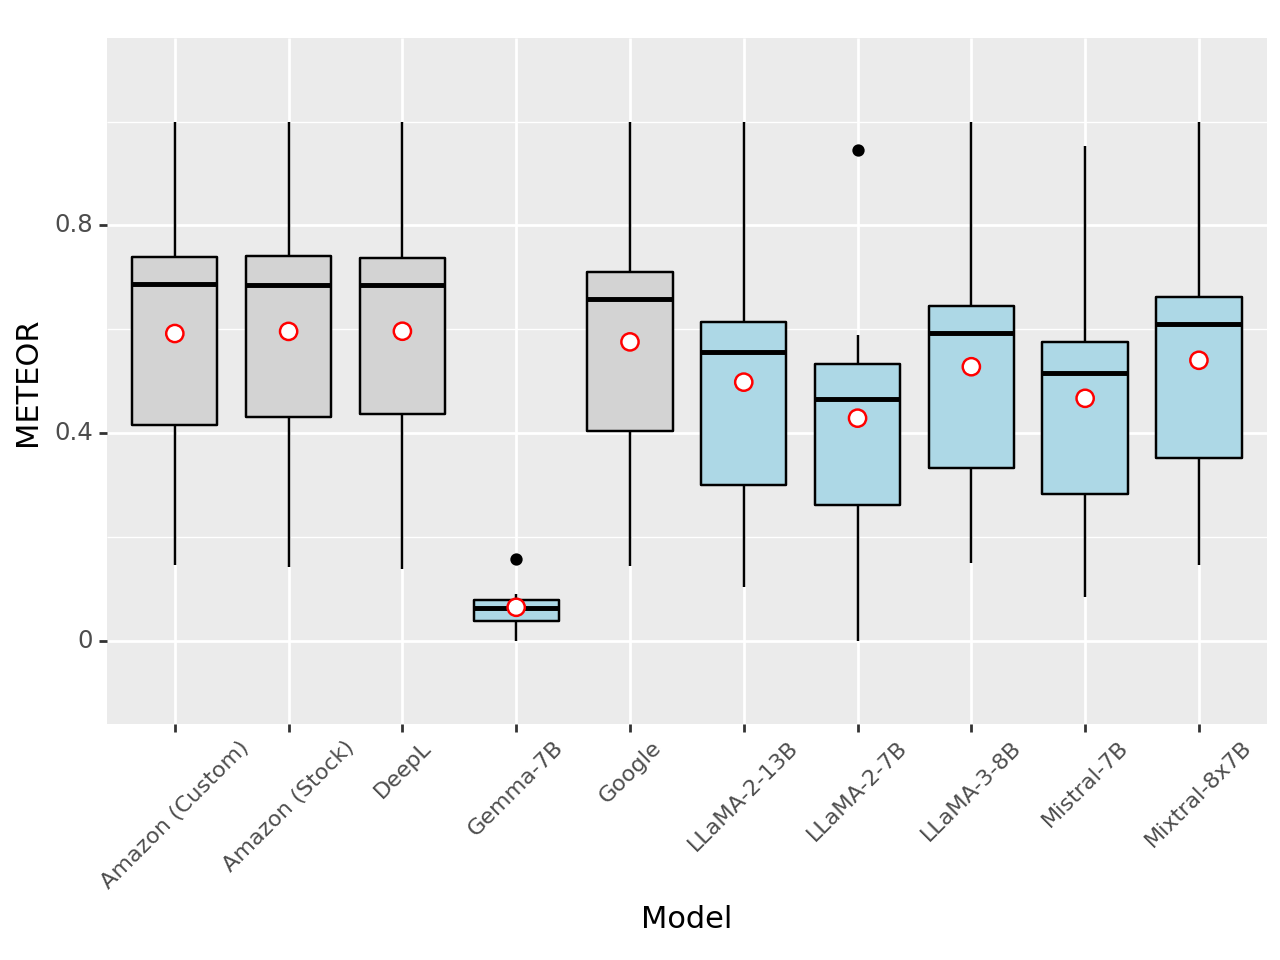
\includegraphics[width=.9\textwidth]{textual/Figuras/Results/Unknown-90.png}
        \caption{Distribution of METEOR Across Models.}
        \label{fig: meteor-models}
\end{figure}


\subsubsection{Mean and median}

When examining the mean (red circles) and median scores (black lines) across METEOR scores for different models, an interesting trend emerges. The mean scores for all models consistently fall a little below the medians, with the medians positioned closer to the upper quartiles, except for Gemma-7B, which shows the mean almost parallel to the median. This pattern suggests that the majority of data points tend to cluster towards higher score ranges, contributing to higher median values. However, the mean scores, possibly influenced by outliers or lower-performing instances, are comparatively lower. This discrepancy indicates potential skewness in the distributions, with some models exhibiting more variability in performance than others.


\subsubsection{Spread of Data}

The IQR (Q3 - Q1) serves as a measure of data dispersion. Across METEOR scores, most models demonstrate similar interquartile sizes, indicating comparable performance variability. Notably, LLaMa-2-7B exhibits a slightly smaller range, while Gemma-7B stands out with a significantly smaller interquartile range, indicating less variability in lower scores. The highest and lowest whiskers in the dataset indicate the range of data distribution among the models. Notably, Gemma-7B and LLaMA-2-7B exhibit the lowest upper whiskers, suggesting a narrower range of performance for these models. Conversely, Google, DeepL and the Amazon models have the highest upper whiskers, indicating a broader spread of performance scores. 

\subsubsection{Outliers}

In Figure~\ref{fig: meteor-models}, only LLaMa-2-7B and Gemma-7B exhibit outliers, marked by black dots above the upper whisker. These outliers indicate significant deviations in performance compared to the bulk of the data, representing exceptionally high scores relative to the majority of data points. Despite their lower scores, Gemma-7B and LLaMa-2-7B stand out as outliers due to the limited number of displayed outliers in the plot.


\subsubsection{Confidence Intervals}

The analysis of CIs for METEOR scores reveals valuable insights into the statistical significance of differences in mean performance across various models. Upon examination of Table~\ref{tab:mean_ci_scores_meteor}, it is evident that the intervals for Amazon (Custom), Amazon (Stock), and DeepL overlap with each other, suggesting that their mean METEOR scores may not be statistically different from one another. On the other hand, the intervals for Gemma-7B, LLaMA-2-13B, LLaMA-3-8B, Mistral-7B, and Mixtral-8x7B do not overlap with those of any other model, indicating potential statistical significance in their performance. 

\begin{table}[htb]
\centering
\begin{tabular}{lccc}
\toprule
\textbf{Model} & \textbf{Mean} & \textbf{CIs} & \textbf{SD} \\
\midrule
Amazon (Custom) & $\mathbf{0.687}$ & [$0.680$, $0.693$] & $0.1468$ \\
Amazon (Stock) & $0.686$ & [$0.679$, $0.693$] & $0.1434$ \\
DeepL & $0.685$ & [$0.679$, $0.692$] & $0.1392$ \\
Gemma-7B & $0.067$ & [$0.066$, $0.068$] & $0.0298$ \\
Google & $0.659$ & [$0.652$, $0.665$] & $0.1440$ \\
LLaMA-2-13B & $0.559$ & [$0.552$, $0.566$] & $0.1596$ \\
LLaMA-2-7B & $0.467$ & [$0.459$, $0.474$] & $0.1730$ \\
LLaMA-3-8B & $0.593$ & [$0.587$, $0.600$] & $0.1495$ \\
Mistral-7B & $0.515$ & [$0.508$, $0.522$] & $0.1556$ \\
Mixtral-8x7B & $0.610$ & [$0.604$, $0.617$] & $0.1461$ \\
\bottomrule
\end{tabular}
\caption{Means, Confidence Intervals (CIs), and Standard Deviations (SD) for METEOR scores.}
\label{tab:mean_ci_scores_meteor}
\end{table}


\subsection{BERTScore Across Models}

Figure~\ref{fig: bertscore-models} depicts model performance using BERTScores. Alongside other statistical measures, these scores offer insights into the quality of the text generated by these models. Unlike metrics like BLEU or METEOR, BERTScore utilizes contextual embeddings from BERT to assess semantic similarity between a generated sentence (candidate) and a reference sentence. By considering contextual information, BERTScore potentially provides more nuanced evaluation. %M: Descrição muito sumária. Coloque ao menos 2 ou 3 linhas explicando em que o BERTscore difere do Meteor. Isso tem de ser feito para todas as métricas. Do contrário, você vai perder o entendimento do leitor.

\begin{figure}[htb]
        \centering
        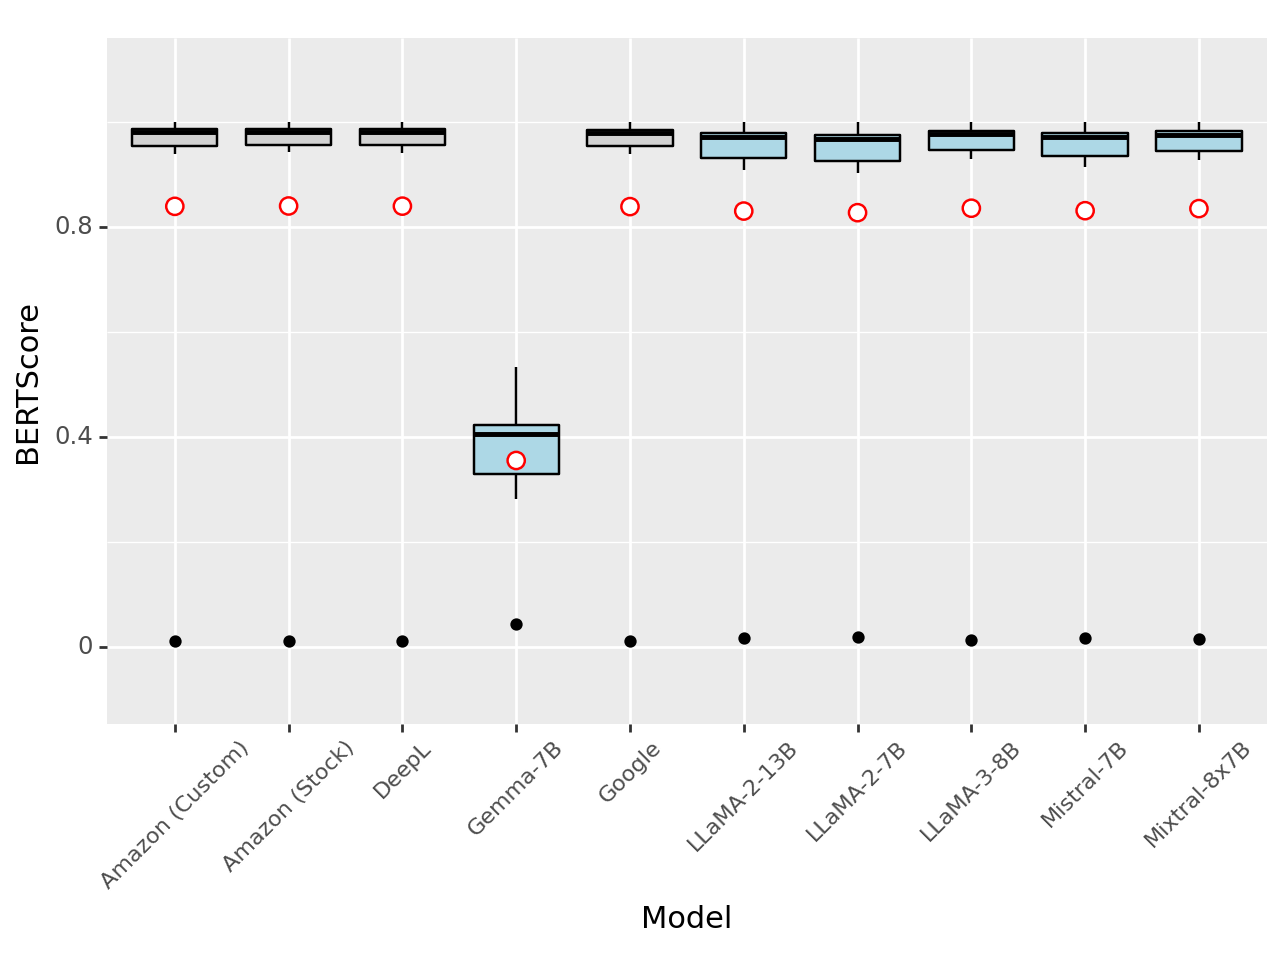
\includegraphics[width=.9\textwidth]{textual/Figuras/Results/Unknown-93.png}
        \caption{Distribution of BERTScore Across Models.}
        \label{fig: bertscore-models}
\end{figure}

        
\subsubsection{Mean and Median}

When comparing the mean (red circles) and median scores (black lines) for BERTScore across different models, noticeable patterns emerge. In most cases, the mean values fall outside the boxplots towards the lower bound, potentially influenced by lower-bound outliers close to zero. This suggests that some outlier data points significantly affect the mean, pulling it towards the lower end of the distribution. Conversely, the medians are consistently positioned very close to the upper quartile bound, indicating that the central tendency of the data lies towards higher score ranges. However, Gemma-7B stands out, with both the mean and median positioned inside the quartile. Interestingly, Gemma-7B's mean is closer to the lower quartile, suggesting a distribution skewed towards lower scores compared to other models.


\subsubsection{Spread of Data}

The IQRs (Q3 -- Q1) provide insights into the spread of data. Gemma-7B stands out with the largest interquartile range compared to other models, despite its lower scores, indicating higher variability in its performance. Conversely, the interquartile ranges for all other models are relatively small and close to 1, suggesting minimal variability in their performance scores. This consistency in interquartile sizes near 1 indicates that the majority of data points for these models fall within a narrow range of scores, contributing to a more consistent performance across different inputs. However, while this highlights consistency, it may also suggest a lack of significant variation among models in terms of their best performance.


\subsubsection{Outliers}

As already discussed, the presence of outliers very close to zero in all models, as seen in Figure~\ref{fig: bertscore-models}, significantly impacts their mean scores, pulling them downwards. These outliers highlight instances where the models struggle with certain inputs, indicating potential challenges in translation accuracy. Addressing these outliers is crucial for enhancing the models' reliability and performance consistency across various inputs and scenarios.


\subsubsection{Confidence Intervals}

The analysis of CIs for BertScore scores reveals notable patterns in mean performance across various models. Overlapping CIs observed among Amazon (Custom), Amazon (Stock), DeepL, and Google, as well as between LLaMA-2-13B and Mistral-7B, and LLaMA-3-8B and Mixtral-8x7B, suggest similar mean BertScore scores. Conversely, non-overlapping intervals for Gemma-7B and LLaMa-2-7B and indicate potential significant differences in their mean BertScore scores compared to other models. These findings underscore the statistical significance of performance variations and emphasize the importance of considering CIs when interpreting BertScore evaluations.

\begin{table}[htb]
\centering
\begin{tabular}{lccc}
\toprule
\textbf{Model} & \textbf{Mean} & \textbf{CIs} & \textbf{SD} \\
\midrule
Amazon (Custom) & $\mathbf{0.980}$ & [$0.979$, $0.981$] & $0.012$ \\
Amazon (Stock) & $\mathbf{0.980}$ & [$0.980$, $0.981$] & $0.012$ \\
DeepL & $\mathbf{0.980}$ & [$0.979$, $0.981$] & $0.012$ \\
Gemma-7B & $0.407$ & [$0.405$, $0.409$] & $0.045$ \\
Google & $0.979$ & [$0.978$, $0.980$] & $0.013$ \\
LLaMA-2-13B & $0.971$ & [$0.970$, $0.972$] & $0.018$ \\
LLaMA-2-7B & $0.966$ & [$0.965$, $0.967$] & $0.020$ \\
LLaMA-3-8B & $0.975$ & [$0.975$, $0.976$] & $0.015$ \\
Mistral-7B & $0.970$ & [$0.969$, $0.971$] & $0.018$ \\
Mixtral-8x7B & $0.974$ & [$0.974$, $0.975$] & $0.015$ \\
\bottomrule
\end{tabular}
\caption{Means, Confidence Intervals (CIs), and Standard Deviations (SD) for BERTScores.}
\label{tab:mean_ci_scores_bert}
\end{table}


\subsection{COMET Across Models}

Figure~\ref{fig: comet-models} utilizes COMET scores to assess the quality of text generated by different models. Unlike metrics like BLEU or METEOR, which focus on \emph{n}-gram overlap, COMET is specifically designed for evaluating translations in conversational contexts. It achieves this by considering various aspects of language important in conversation, such as fluency, relevance, and specificity. To make these judgments, COMET employs pre-trained models.

\begin{figure}[htb]
        \centering
        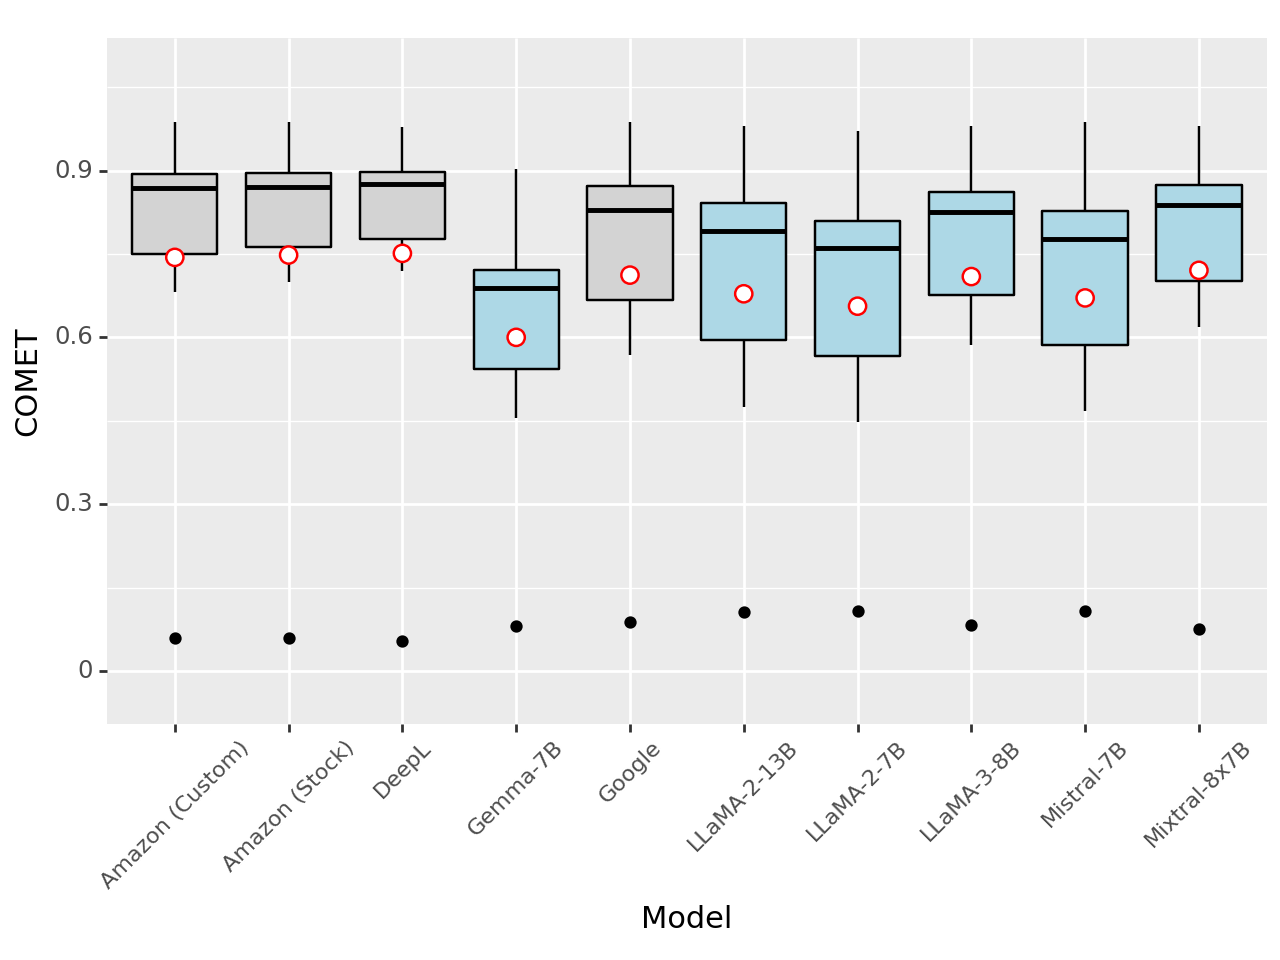
\includegraphics[width=.9\textwidth]{textual/Figuras/Results/Unknown-94.png}
        \caption{Distribution of COMET Across Models.}
        \label{fig: comet-models}
\end{figure}


\subsubsection{Mean and Median}

The analysis of means and medians reveals a consistent trend across models, with medians (black lines) consistently positioned near the upper quartile, indicating a concentration of data in higher score ranges. However, the means (red circles) vary among models, some appearing very close to the lower quartile, such as Google, Mixtral-8x7B, and LLaMa-3-8B, while others fall slightly outside the interquartile range, notably observed in the Amazon models and DeepL. This suggests potential negative skewness in certain distributions and underscores the importance of carefully considering outlier effects in data analysis.


\subsubsection{Spread of Data}

Analyzing the spread of data and interquartile ranges (Q3 - Q1) across models provides insights into the variability of COMET scores. The interquartile ranges vary less across models, indicating similarities in data spread and performance consistency. Among NMT providers, Amazon and DeepL exhibit overlapping interquartile ranges, suggesting similarity in performance, while Google shows more variability. Interestingly, among LLMs, Mixtral-8x7B and LLaMa-3-8B present overlaps with Google, suggesting similarities in score distributions. Conversely, Gemma-7B displays the lowest-positioned interquartile range, indicating more consistent performance, but with lower scores.


\subsubsection{Outliers}

The existence of outliers, as depicted in Figure~\ref{fig: comet-models}, substantially influences the mean scores, causing them to decrease. These outliers indicate situations where the models encounter difficulties with specific inputs, suggesting potential challenges in translation accuracy. It is essential to address these outliers to improve the reliability and consistency of the models' performance across different inputs and scenarios.


\subsubsection{Confidence Intervals}

The examination of CIs offers valuable insights into the statistical significance of performance differences among models. Referring to Table~\ref{tab:mean_ci_scores_comet}, it becomes apparent that the intervals for LLaMA-3-8B and Google, along with those for Amazon (Stock) and Amazon (Custom), overlap. This overlap suggests that the mean scores of these models may not exhibit statistically significant differences. Conversely, Gemma-7B, LLaMA-2-13B, LLaMA-3-8B, Mistral-7B, and Mixtral-8x7B show non-overlapping confidence intervals, indicating potential significant distinctions in their mean scores. 

\begin{table}[htb]
\centering
\begin{tabular}{lccc}
\toprule
\textbf{Model} & \textbf{Mean} & \textbf{CIs} & \textbf{SD} \\
\midrule
Amazon (Custom) & $0.870$ & [$0.869$, $0.871$] & $0.059$ \\
Amazon (Stock) & $0.871$ & [$0.868$, $0.874$] & $0.058$ \\
DeepL & $\mathbf{0.875}$ & [$0.873$, $0.878$] & $0.053$ \\
Gemma-7B & $0.688$ & [$0.685$, $0.692$] & $0.081$ \\
Google & $0.830$ & [$0.826$, $0.834$] & $0.088$ \\
LLaMA-2-13B & $0.791$ & [$0.787$, $0.796$] & $0.107$ \\
LLaMA-2-7B & $0.761$ & [$0.757$, $0.766$] & $0.108$ \\
LLaMA-3-8B & $0.826$ & [$0.822$, $0.830$] & $0.081$ \\
Mistral-7B & $0.777$ & [$0.773$, $0.781$] & $0.107$ \\
Mixtral-8x7B & $0.840$ & [$0.837$, $0.842$] & $0.075$ \\
\bottomrule
\end{tabular}
\caption{Means, Confidence Intervals (CIs), and Standard Deviations (SD) for COMET scores.}
\label{tab:mean_ci_scores_comet}
\end{table}


\subsection{TER Across Models}

Figure~\ref{fig: ter-models} depicts model performance based on TER scores. These scores, combined with other statistical measures, provide insights into the quality of text generated by the models. Unlike metrics that focus on similarity (BLEU, METEOR) or contextual understanding (BERTScore, COMET), TER takes a different approach. It measures the number of edits required to transform a machine translation into a reference translation. This simple and efficient method, however, has limitations. TER struggles to capture semantic differences between the original text and the translations, potentially overlooking quality issues.

\begin{figure}[htb]
        \centering
        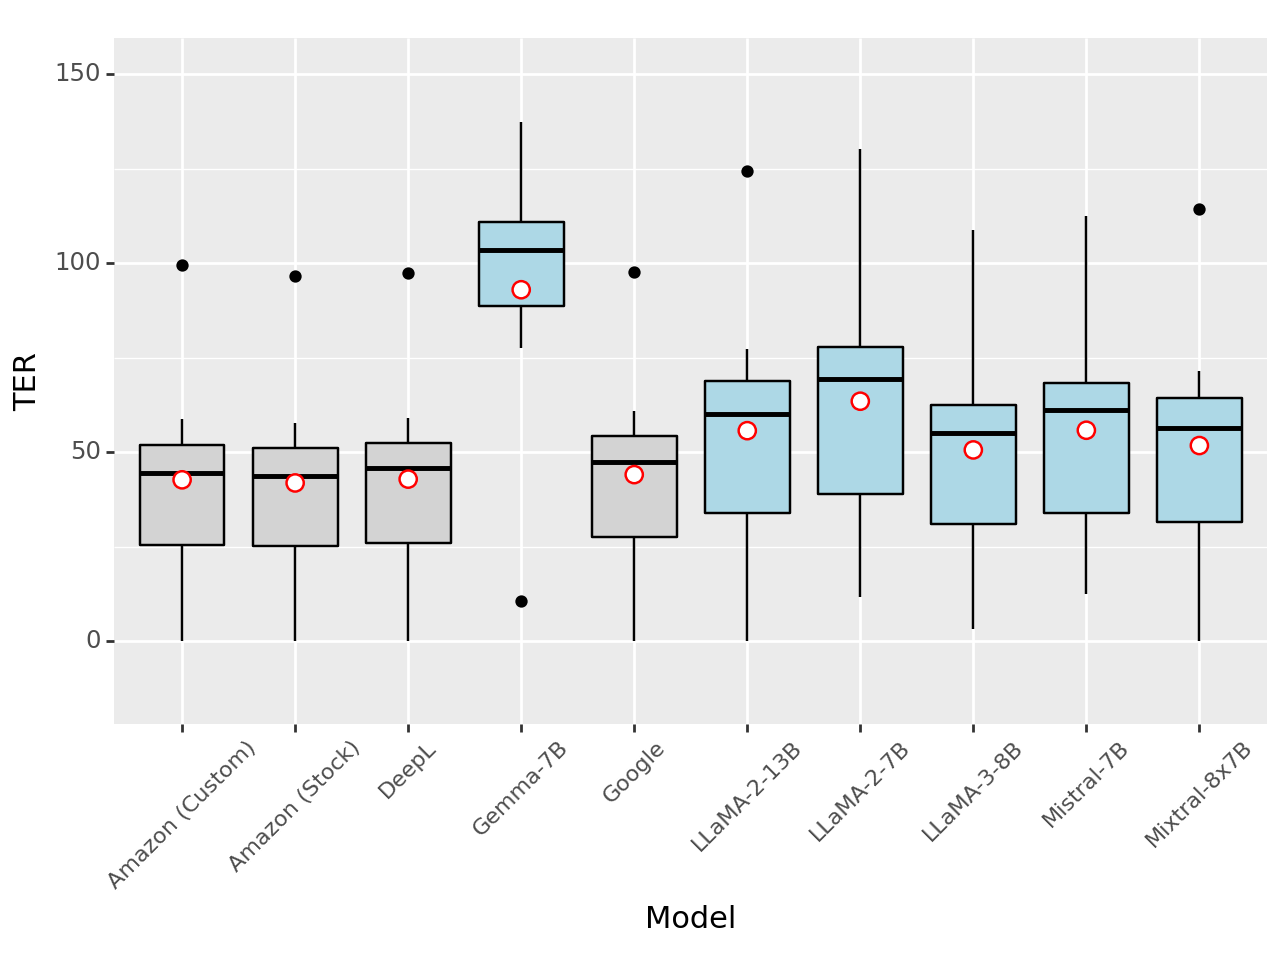
\includegraphics[width=.9\textwidth]{textual/Figuras/Results/Unknown-95.png}
        \caption{Distribution of TER Across Models.}
        \label{fig: ter-models}
\end{figure}
        

\subsubsection{Mean and Median}

The analysis of mean and median scores highlights a consistent trend observed across models, with medians (represented by black lines) consistently situated near the upper quartile. This implies a concentration of data in higher score ranges. However, the influence of outliers on means (depicted by red circles) varies across models, pulling them either very close to the median and upper quartile, as seen in most models, or to the lower quartile, particularly noticeable in Gemma-7B. This suggests potential negative skewness in certain distributions, highlighting the need for careful consideration of outlier effects in data analysis.


\subsubsection{Spread of Data}

The IQR, calculated as Q3 - Q1, provides insight into the spread of data within the middle 50\% of observations. Models like LLaMA-2-13B, LLaMA-2-7B, and Mistral-7B have wider IQRs (around $31.337$, $29.641$, and $25.000$ respectively), suggesting more variability in their TER scores. Conversely, models such as Gemma-7B have narrower IQRs (around $15.000$), indicating less variability. Gemma-7B as well as LLaMA-2-7B exhibit the highest whisker values (around $137.500$ and $130.175$ respectively), implying higher scores, which in this case means lower performance compared to the other models. Conversely, LLaMA-2-7B has the lowest whisker values (around $0.00$). These extreme values highlight potentially influential data points beyond the quartiles.


\subsubsection{Outliers}

As depicted in Figure~\ref{fig: ter-models}, outliers noticeably affect model performance assessment in the dataset. Across most models, outliers tend to elevate the mean TER scores closer to the upper quartile, indicating higher translation errors. However, in Gemma-7B, outliers pull the mean TER score closer to the lower quartile, suggesting unusually low translation errors, which in this case mean good translations. This disparity underscores the diverse impact of outliers on model evaluation, highlighting the complexity of interpreting model performance amidst the presence of outliers.


\subsubsection{Confidence Intervals}

Analyzing mean TER scores and their confidence intervals reveals patterns of overlap and distinctiveness among models, as illustrated in Table~\ref{tab:mean_ci_scores_ter}. LLaMA-3-8B and Mixtral-8x7B, as well as other pairs such as Amazon (Custom) and Amazon (Stock), and Mistral-7B and LLaMA-2-13B, demonstrate overlapping confidence intervals, suggesting potential similarity in their performance. Conversely, Gemma-7B and LLaMA-2-7B exhibit distinct intervals, hinting at differences in their mean TER scores. Particularly, Gemma-7B stands out with a notably higher mean and non-overlapping interval, indicating the lowest performance and potential statistical significance compared to other models.

\begin{table}[htb]
\centering
\begin{tabular}{lccc}
\toprule
\textbf{Model} & \textbf{Mean} & \textbf{CIs} & \textbf{SD} \\
\midrule
Amazon (Custom) & $44.709$ & [$43.850$, $45.569$] & $19.257$ \\
Amazon (Stock) & $\mathbf{44.438}$ & [$43.612$, $45.265$] & $18.621$ \\
DeepL & $45.676$ & [$44.844$, $46.508$] & $18.678$ \\
Gemma-7B & $106.799$ & [$106.319$, $107.278$] & $10.663$ \\
Google & $47.501$ & [$46.676$, $48.327$] & $18.508$ \\
LLaMA-2-13B & $60.403$ & [$59.414$, $61.392$] & $21.803$ \\
LLaMA-2-7B & $69.953$ & [$68.986$, $70.919$] & $21.510$ \\
LLaMA-3-8B & $55.700$ & [$54.855$, $56.546$] & $18.963$ \\
Mistral-7B & $61.271$ & [$60.481$, $62.062$] & $17.651$ \\
Mixtral-8x7B & $56.251$ & [$55.345$, $57.157$] & $20.176$ \\
\bottomrule
\end{tabular}
\caption{Means, Confidence Intervals (CIs), and Standard Deviations (SD) for TER scores.}
\label{tab:mean_ci_scores_ter}
\end{table}



\section{Manual Error Analysis}
\label{sec: Error-analysis}

In this section, we present the results of the human evaluation step. As described in Section~\ref{sec: Human Evaluation}, 10\% of the data (200 segments) were randomly selected for manual error classification. The labels used for error categorization were described in Table~\ref{tab: error_categories}.


\subsection{Analysis by Model: Correct Translations vs. Errors}

Models were initially evaluated based on their overall ability to produce correct translations while minimizing errors. Table~\ref{tab:corrects_errors_summary} provides a summary of the total of correct translations and errors for different models. Here, this analysis helps us understand how different LLMs performed individually and compared to traditional NMT systems.

\begin{table}[htb]
\centering
\begin{tabular}{lcccc}
\toprule
& \multicolumn{2}{c}{\textbf{Total of}} & \multicolumn{2}{c}{\textbf{\% of}} \\
\cmidrule(lr){2-3} \cmidrule(lr){4-5}
\textbf{Model} & \textbf{CC} & \textbf{ER} & \textbf{CC} & \textbf{ER} \\
\midrule
DeepL & $156$ & $44$ & $78.00\%$ & $22.00\%$ \\
\midrule
Gemma-7B & $46$ & $282$ & $14.02\%$ & $85.98\%$ \\
LLaMA-2-13B & $26$ & $333$ & $7.24\%$ & $92.76\%$ \\
LLaMA-2-7B & $19$ & $\mathbf{421}$ & $4.31\%$ & $95.68\%$ \\
LLaMA-3-8B & $45$ & $232$ & $16.25\%$ & $83.75\%$ \\
Mistral-7B & $16$ & $374$ & $4.10\%$ & $\mathbf{95.90\%}$ \\
Mixtral-8x7B & $\mathbf{71}$ & $177$ & $\mathbf{28.63}\%$ & $71.37\%$ \\
\bottomrule
\end{tabular}
\caption{Summary of Correct Translations (CC) vs. Errors (ER) by Model.}
\label{tab:corrects_errors_summary}
\end{table}


The analysis of correct translations vs. errors reveals that DeepL, an NMT system, significantly outperformed all LLMs, achieving $156$ ($78\%$) correct translations and $44$ ($22\%$) errors. Among LLMs, Mixtral-8x7B demonstrated the best performance with $71$ ($\approx29\%$) correct translations and $177$ ($\approx71\%$) errors. Gemma-7B and LLaMA-3-8B exhibited the second and third highest performance, with $46$ ($\approx14\%$) and $45$ ($\approx16\%$) correct translations, respectively. Notably, Gemma-7B had considerably more errors than LLaMA-3-8B, with $50$ ($2.26\%$) more errors. Meanwhile, LLaMA-2-13B, LLaMA-2-7B, and Mistral-7B showed the lowest performance, with correct translation percentages ranging from $\approx4\%$ to $\approx16\%$. Particularly, Mistral-7B presented the highest proportion of errors ($\approx96\%$) among LLMs. We emphasize that a `correct' translation does not contain errors of any type. In Table~\ref{tab:corrects_errors_summary}, values in bold indicate the models with the best and worst performance among the LLMs. This analysis emphasizes the need for further improvement in LLMs to compete with traditional NMT systems in terms of translation accuracy.


\subsection{Analysis by Model: Spatial vs. Non-spatial \& Other Errors}

Models were then assessed based on subgroups of error types to gain a better understanding of the relationship between different models and specific types of errors. Table~\ref{tab:model_performance_by_error_type} provides a summary of the number of errors grouped into spatial, non-spatial, and other categories.

\begin{table}[htb]
\centering
\begin{tabular}{lcccccc}
\toprule
& \multicolumn{3}{c}{\textbf{Total of Errors}} & \multicolumn{3}{c}{\textbf{\% of Errors}} \\
\cmidrule(lr){2-4} \cmidrule(lr){5-7}
\textbf{Model} & \textbf{SP} & \textbf{N-SP} & \textbf{OE} & \textbf{SP} & \textbf{N-SP} & \textbf{OE} \\
\midrule
DeepL & $8$ & $13$ & $23$ & $\mathbf{21.62\%}$ & $\mathbf{35.14}\%$ & $43.24\%$ \\
\midrule
Gemma-7B & $11$ & $25$ & $246$ & $4.09\%$ & $9.29\%$ & $86.62\%$ \\
LLaMA-2-13B & $16$ & $32$ & $285$ & $6.19\%$ & $7.71\%$ & $86.10\%$ \\
LLaMA-2-7B & $\mathbf{25}$ & $31$ & $365$ & $4.17\%$ & $5.17\%$ & $\mathbf{90.67\%}$ \\
LLaMA-3-8B & $18$ & $31$ & $183$ & $5.36\%$ & $10.77\%$ & $83.87\%$ \\
Mistral-7B & $20$ & $\mathbf{38}$ & $\mathbf{316}$ & $5.33\%$ & $10.11\%$ & $84.56\%$ \\
Mixtral-8x7B & $17$ & $30$ & $130$ & $\mathbf{9.14\%}$ & $\mathbf{16.13\%}$ & $74.73\%$ \\
\bottomrule
\end{tabular}
\caption{Comparison of Spatial (SP) vs. Non-spatial (N-SP) and Other Errors (OE) by Model.}
\label{tab:model_performance_by_error_type}
\end{table}

The analysis of Table~\ref{tab:model_performance_by_error_type} reveals a complex relationship between models and error categories. While a strong correlation between model robustness and overall performance might be expected, a closer look is needed. Examining the table, we can observe a trend where LLMs tend to have a predominance of non-spatial errors and a considerably higher number of other errors compared to DeepL. For instance, Mistra-7B had the biggest number of non-spatail errors ($38$), as well as other errors ($316$), while the biggest proportions were obtained by DeepL, with $\approx35\%$, and LLaMa-2-7B, with  $1\approx91\%$.

The table also reveals a variation in the total number of spatial errors across models. DeepL, the only NMT system, despite having the fewest number ($8$), has the highest proportion ($\approx22\%$) of spatial errors. This means that its relatively small number of spatial errors affected model performance more compared to LLMs. Conversely, among LLMs, LLaMA-2-7B has the lowest proportion ($\approx5\%$), followed by LLaMA-2-13B with $\approx8\%$. Interestingly, Mixtral-8x7B did not vary considerably between spatial and non-spatial errors but showed the best performance in handling other errors, with $130$ ($\approx75\%$).

These findings suggest a potential trend: current open-source LLMs might be more susceptible to translation errors in general, including both spatial and non-spatial errors, compared to NMT systems. Even when some LLMs have similar total error rates, a closer look reveals a bias towards non-spatial errors. This underlines the importance of considering error proportions, not just total error count, for a comprehensive evaluation of model performance.


\subsection{Analysis by Model: Exploring All Error Types}

Taking the analysis a step further, we examine whether different models exhibit a propensity for specific error types. Figure~\ref{fig: error-types} provides a detailed breakdown of the total number of specific errors types by model (please, refer back to Table~\ref{tab: error_categories} for the complete description of error categories). Our aim is to identify potential patterns in error distribution across models to gain a deeper understanding of their strengths and weaknesses.

\begin{figure}[htb]
        \centering
        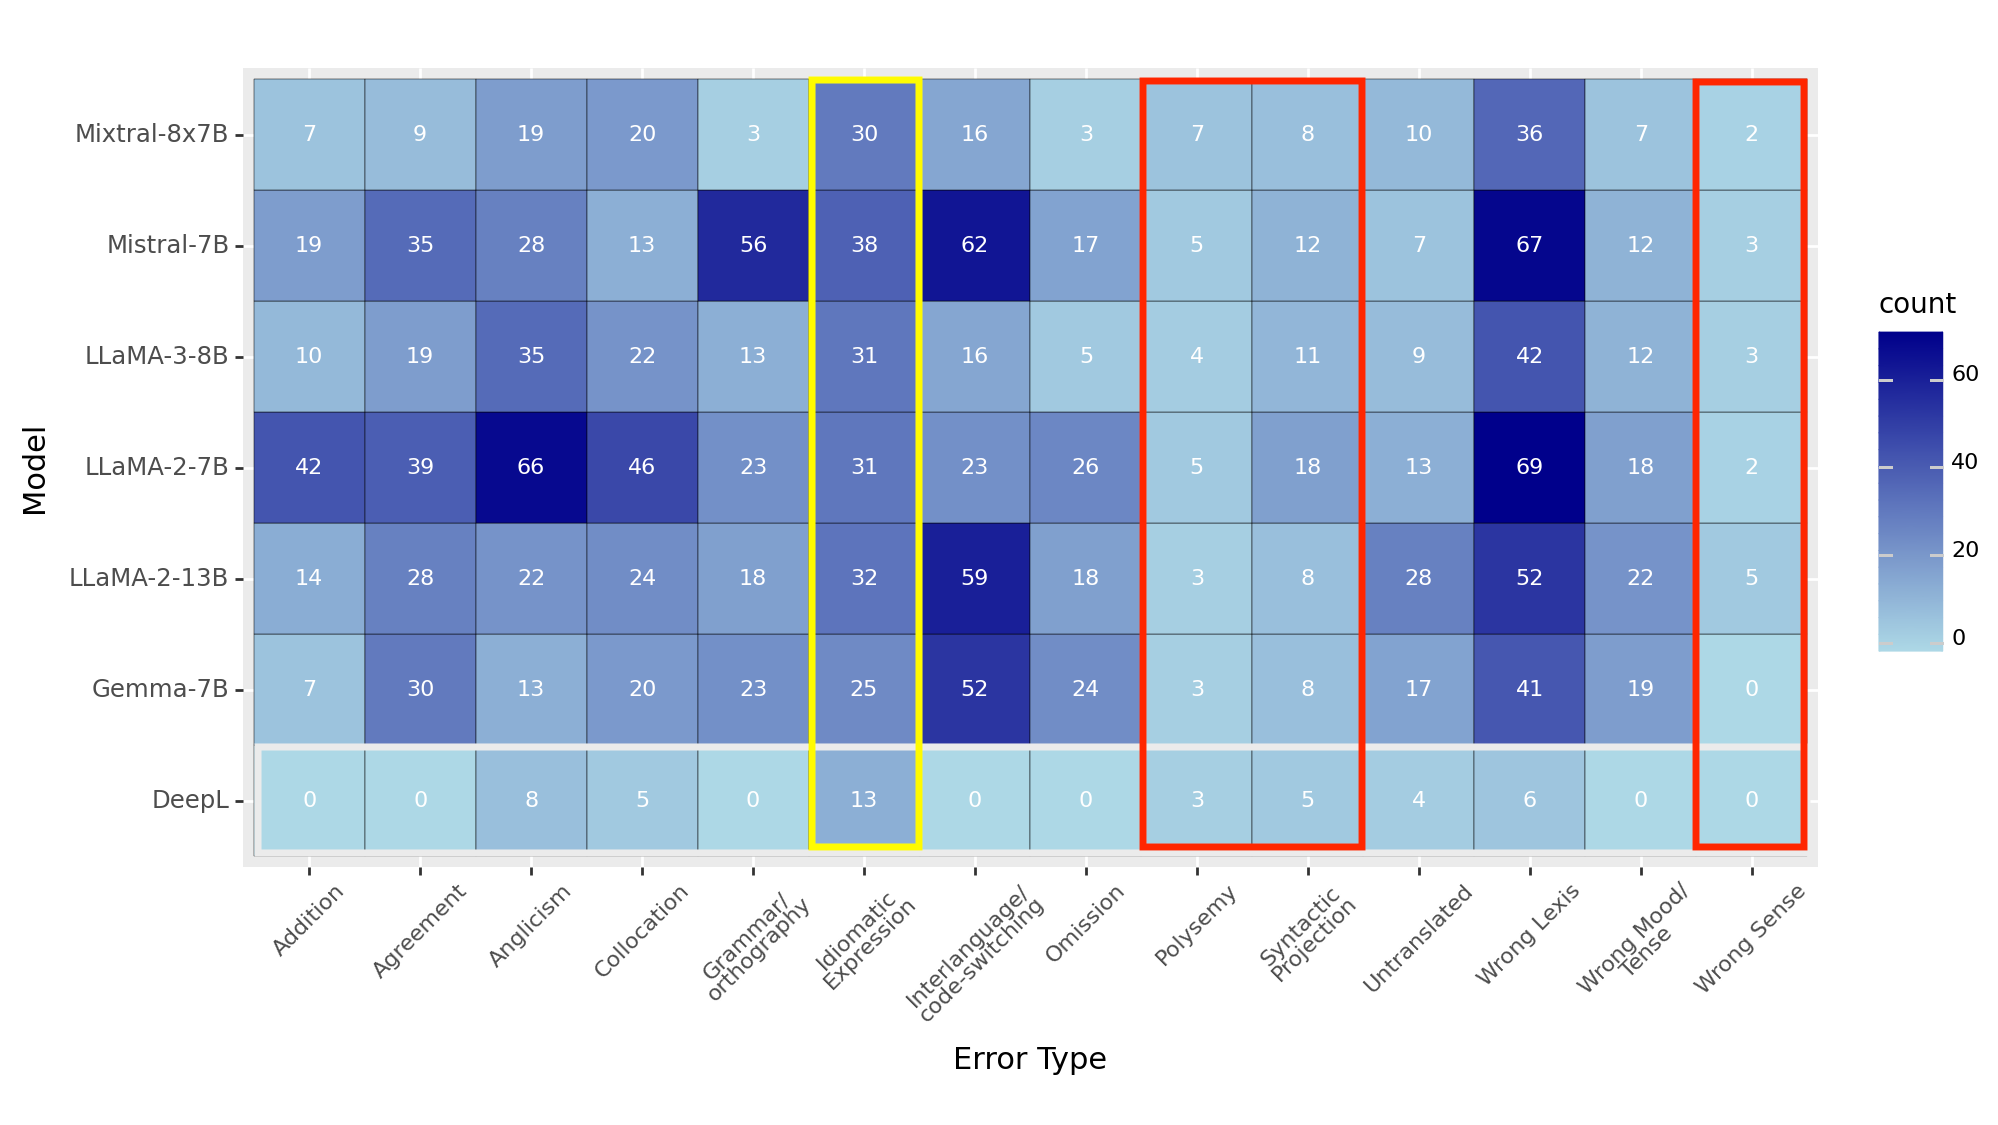
\includegraphics[width=1\textwidth]{textual/Figuras/Results/Unknown-44.png}
        \caption{Distribution of All Error Types by Model (Count).}
        \label{fig: error-types}
\end{figure}

The heatmap in Figure~\ref{fig: error-types} offers insights into the distribution of general and spatial errors across various models. As delineated in Subsection~\ref{subsec: Manual Error Classification}, spatial errors (highlighted in red), the core of our investigation, encompass polysemy (po), syntactic projection (sp), and wrong sense (ws). Additionally, our focus extends to examining idiomatic expression (ie) errors (highlighted in yellow). DeepL (highlighted in white) was the only NMT system taken to human review. By observing the intensity and color gradient for each error type within the heatmap, we can spot potential patterns in model behavior.


\subsubsection{Spatial Errors}

Spatial errors refer to mistranslation errors where a model fails to understand or represent correct spatial relationships. Figure~\ref{fig: error-types} reveals that, among LLMs, spatial errors had some of the smallest distributions compared to general non-spatial errors (with some numbers being similar to DeepL for polysemy (po) issues, for instance). However, we would like to emphasize that this finding does not mean LLMs are less prone to spatial errors. On the contrary, some LLMs exhibited more than triple the number of syntatic projection (sp) errors compared to DeepL. Instead, it suggests that LLMs presented a wider variety of serious issues, among which a much larger proportion were non-spatial.

Among LLMs, Mixtral-8x7B, Mistral-7B, and LLaMa-2-7B presented the highest number of polysemy (po) errors, with $7$, $5$, and $5$ errors, respectively. LLaMa-2-7B ($18$ errors), Mistral-7B ($12$ errors), and LLaMa-3-8B ($11$ errors) presented the highest number of syntactic projection (sp) errors. For wrong sense (ws) errors, LLaMa-2-13B presented the highest number, with $5$ in total, followed by LLaMa-3-8B, also with $5$. This indicates that, for some models like LLaMa-2-7B, Mistral-7B, and LLaMa-3-8B, spatial errors were particularly problematic. Examples~\ref{ex:ex-1}, \ref{ex:ex-2}, and \ref{ex:ex-3} illustrate these three error types.

\ex.\texttt{(inner\_id: 70115)} \hfill \texttt{Into(i)} \\[0.3ex] 
\noindent\rule{\linewidth}{0.9pt}
In between those two \textcolor{blue}{landmarks} in Ham's life, he \colorbox{lightblue}{\textcolor{blue}{flew}} \colorbox{lightgray}{\emph{\textcolor{blue}{into}}} space. (SRC) \label{ex:ex-1} \\[-0.3ex] 
\noindent\rule{\linewidth}{0.3pt}
Entre esses dois \textcolor{ForestGreen}{marcos} da vida de Ham, ele \colorbox{lightgray}{\textcolor{ForestGreen}{foi}} \colorbox{lightgray}{\textcolor{ForestGreen}{\emph{ao}}} espaço. (REF) \\[-0.3ex]
\noindent\rule{\linewidth}{0.3pt}
*~Entre esses dois \textcolor{Maroon}{marcadores} da vida de Ham, ele \colorbox{lightblue}{\textcolor{Maroon}{voou}} \colorbox{lightgray}{\textcolor{Maroon}{\emph{para}}} o espaço. (Mistral-7B) \\[-0.3ex] 
\noindent\rule{\linewidth}{0.9pt}

\ex.\texttt{(inner\_id: 65421)} \hfill \texttt{Into(i)} \\[0.3ex] 
\noindent\rule{\linewidth}{0.9pt}
I'd like to take you on a journey \colorbox{lightgray}{\emph{\textcolor{blue}{into}}} the sea, looking at it from the perspective of its smallest inhabitants: the microbes. (SRC)\label{ex:ex-2} \\[-0.3ex]  
\noindent\rule{\linewidth}{0.3pt}
Eu gostaria de levá-los em uma jornada \colorbox{lightgray}{\emph{\textcolor{ForestGreen}{pelo}}} mar, olhando pela perspectiva de seus menores habitantes: os micróbios. (REF) \\[-0.3ex] 
\noindent\rule{\linewidth}{0.3pt}
*~Gostaria de levar você em uma jornada \colorbox{lightgray}{\emph{\textcolor{Maroon}{para}}} o fundo do mar, observando-o pela perspetiva de seus menores habitantes: os microrganismos. (Gemma-7B) \\[-0.3ex] 
\noindent\rule{\linewidth}{0.9pt}

As observed in Examples~\ref{ex:ex-1} and \ref{ex:ex-2}, both Mistral-7B and Gemma-7B incorrectly translate the preposition ``into'' as ``para''. A more accurate choice would be ``ao,'' which conveys the idea of going to a place or space for a short period of time. In PT-br, ``para'' typically suggests movement with permanence in the target location, which is not observed in the source sentences. Specifically, Example~\ref{ex:ex-2} is a case of polysemy (po), because ``para'' is indeed a possible sense for ``into'', but not the appropriate one. Example~\ref{ex:ex-1} exemplifies a case of syntactic projection (sp) error due to its projection of English spatial constructions to PT-br. Here, not only is the preposition ``into'' misinterpreted as ``para'', but also the English Manner verb ``flew'' is directly projected to its PT-br counterpart ``voou'' (flew). This syntactic construction, combining a Manner verb (``fly'') with a Path preposition (``into''), as described by~\textcite{Talmy00_2, slobin2005relating}, does not align with the expected lexicalization patterns for the spatial description of this scene in PT-br. Furthermore, the word choice ``marcadores'' constitutes a wrong lexical choice (wl).

In contrast, Example~\ref{ex:ex-3} illustrates a case of wrong sense (ws) error because, unlike in \ref{ex:ex-1} and \ref{ex:ex-2}, where the preposition's sense was correct but not appropriate, here the sense might sound appropriate, but is not the correct idea conveyed by the EN preposition.

\ex.\texttt{(inner\_id: 26335)} \hfill \texttt{Across(iv)} \\[0.3ex] 
\noindent\rule{\linewidth}{0.9pt}
Because the Internet and connection technologies are connecting them \colorbox{lightgray}{\emph{\textcolor{blue}{across}}} the world. (SRC)\label{ex:ex-3} \\[-0.3ex] 
\noindent\rule{\linewidth}{0.3pt}
Porque a Internet e as tecnologias de conexão estão ligando-os \colorbox{lightgray}{\emph{\textcolor{ForestGreen}{por todo}}} o mundo. (REF) \\[-0.3ex]
\noindent\rule{\linewidth}{0.3pt}
*~Porque a Internet e as tecnologias de conexão estão conectando-os \colorbox{lightgray}{\emph{\textcolor{Maroon}{ao redor}}} do mundo. (LLaMa-2-13B) \\[-0.3ex] 
\noindent\rule{\linewidth}{0.9pt}

Unlike in Examples~\ref{ex:ex-1} and \ref{ex:ex-2}, where ``para'' was one of the possible meaning for ``into'', here ``ao redor'' (around) conveys a slightly different concept than ``across''. The correct meaning ``por todo'' (throughout) conveys the idea of distribution present in the source sentence. To better understand this difference, if the expression ``around/across the world'' is not clear, we suggest changing to ``the USA'', and translating to PT-br. ``Ao redor dos EUA'' (around the USA) conveys a rather different concept, indicating a circular or curved motion/location \parencite{dicioRedor}, whereas ``por todo os EUA'' (across the USA) indicates that the connection is spread or occupying the whole surface of country \parencite{bruckfield2011prepositions}. 


\subsubsection{Non-Spatial \& Other Errors}

`Non-spatial' errors refer to mistranslation errors involving idiomatic expressions, i.e., specifically EN phrasal verbs and idioms that contain spatial prepositions in non-spatial senses. Conversely, `Other errors' encompass a broader spectrum of issues beyond misinterpretations. This category includes addition (ad), omission (om), collocation (co), anglicism (an), wrong lexical choice (wl), as well as interlanguage/code-switching (cs).

The analysis of Figure~\ref{fig: error-types} revealed that Other errors were prevalent across LLMs, with LLaMa-2-7B and Mistral-7B exhibiting the highest numbers. Particularly, LLaMa-2-7B (see Example~\ref{ex:ex-4}) primarily struggled with wrong lexical choice ($69$ errors), where it selected inappropriate words despite being grammatically correct. Additionally, it frequently used anglicisms ($66$ errors), directly translating English phrases into  PT-br, resulting in unnatural phrasing. Finally, LLaMa-2-7B also made collocation errors, using grammatically correct words that lacked the intended meaning in PT-br.

\ex.\texttt{(inner\_id: 73959)} \hfill \texttt{Into(iii)} \\[0.3ex]
\noindent\rule{\linewidth}{0.9pt}
You can always \colorbox{lightgray}{fool yourself \emph{\textcolor{blue}{into}} seeing} a decline if you compare \textcolor{blue}{bleeding headlines} of the present with \textcolor{blue}{rose-tinted} images of the past. (SRC) \label{ex:ex-4} \\[-0.3ex]
\noindent\rule{\linewidth}{0.3pt}
Você sempre pode \colorbox{lightgray}{enganar a si mesmo \emph{\textcolor{ForestGreen}{e}} ver} um declínio se comparar as  \textcolor{ForestGreen}{manchetes sangrentas} dos dias atuais com as lembranças \textcolor{ForestGreen}{cor-de-rosa} do passado. (REF) \\[-0.3ex]
\noindent\rule{\linewidth}{0.3pt}
?~Você pode sempre \colorbox{lightgray}{enganar-se \emph{\textcolor{Maroon}{em}} ver} uma decadência se comparar os \textcolor{Maroon}{títulos de jornal sangrando} do presente com imagens \colorbox{lightyellow}{\emph{\textcolor{Maroon}{rosa-tintadas}}} do passado. (LLaMa-2-7B) \\[-0.3ex] 
\noindent\rule{\linewidth}{0.9pt}


As can be seen in Example~\ref{ex:ex-4}, the translation ``enganar-se \emph{em} ver'' displays an anglicism (an), where the PT-br expression is directly transposed from the EN phrase. The particular issue lies in the translation of ``into'' as ``em''. In this context, a more suitable choice would be ``a,'' or the translation may necessitate a coordinated clause with ``e,'' similar to the structure utilized by the human translator. Additionally, ``jornal sangrando'' is an instance of wrong lexical choice (wl) error, and ``rosa-tintadas'' is a case of interlanguage/code-switching (in) error, as this phrase does not exist in PT-br.

Mistral-7B showcased a distinct error profile. Like LLaMa-2-7B, it encountered difficulties in selecting the most appropriate words (wrong lexical choice (wl), $67$ errors) and grappled with grammar/orthography (gr) ($56$ errors). However, its second most prevalent error type was interlanguage/code-switching (in) ($62$ errors), where it either generated new words or unintentionally mixed up PT-br with other languages, such as Spanish, within the translations. LLaMa-2-13B and Gemma-7B also exhibit this category of errors. Example~\ref{ex:ex-5} illustrates another case of interlanguage/code-switching error, where ``segreda'' is another made-up word in PT-br. It is also worth saying that ``por meio de'' would be a better lexical choice showing idiomaticity in PT-br instead of ``através de''.

\ex.\texttt{(inner\_id: 18009)} \hfill  \texttt{Through(v)}\\[0.3ex]
\noindent\rule{\linewidth}{0.9pt}
And they do it \colorbox{lightgray}{\textcolor{blue}{secretly}} \emph{through} misinformation and ambiguities and irrelevancies, trying to cause everyone to think more deeply. (SRC) \label{ex:ex-5} \\[-0.3ex]
\noindent\rule{\linewidth}{0.3pt}
E ele faz isso \colorbox{lightgray}{\textcolor{ForestGreen}{em segredo}} \emph{através de} informações incorretas e ambiguidades e irrelevâncias, tentando fazer com que todos pensem mais. (REF) \\[-0.3ex]
\noindent\rule{\linewidth}{0.3pt}
?~E eles fazem isso \colorbox{lightgray}{de forma \emph{\textcolor{Maroon}{segreda}}} \emph{através de} desinformações e ambiguidades e irrelevâncias, tentando fazer todos pensar mais profundamente. (Mistral-7B) \\[-0.3ex] 
\noindent\rule{\linewidth}{0.9pt}


Besides wrong lexical choice (wl) errors, anglicism (an) and collocation (co) errors were also among the most common error types across various models, with LLaMa-2-7B being the primary contributor in both categories. LLaMa-3-8B followed, with $35$ anglicism errors and $22$ collocation errors, while LLaMa-2-13B had $22$ anglicism errors and $24$ collocation errors. Example~\ref{ex:ex-6} showcases instances of these errors. The EN phrase ``so that night'' is literally translated to ``assim que noite,'' which is an anglicism (an) error. Additionally, ``empacotei em uma sacola'' is not the correct combination for ``pack in a bag,'' constituting both a collocation (co) and a wrong lexical choice (wl) error. Lastly, ``caminhei até'' is another case of syntactic projection (sp) in PT-br.


\ex.\texttt{(inner\_id: 11977)} \hfill \texttt{Into(i)}\\[0.3ex]
\noindent\rule{\linewidth}{0.9pt}
\colorbox{lightyellow}{\textcolor{blue}{So that night}}, I \colorbox{lightgray}{\textcolor{blue}{packed} all my things in a \textcolor{blue}{bag}}, and I \colorbox{lightblue}{\textcolor{blue}{walked}} \colorbox{lightgray}{\emph{\textcolor{blue}{into}}} my father's \colorbox{lightgray}{\textcolor{blue}{room}} and told him, ``Tomorrow morning, the bus is going to come in''. (SRC) \label{ex:ex-6} \\[-0.3ex]
\noindent\rule{\linewidth}{0.3pt}
\colorbox{lightgray}{\textcolor{ForestGreen}{Naquela noite}}, \colorbox{lightgray}{\textcolor{ForestGreen}{fiz} minha \textcolor{ForestGreen}{mala}}, \colorbox{lightgray}{\emph{\textcolor{ForestGreen}{entrei} no}} \colorbox{lightgray}{\textcolor{ForestGreen}{quarto}} do meu pai e disse: ``Amanhã cedo o ônibus vai passar''. (REF) \\[-0.3ex]
\noindent\rule{\linewidth}{0.3pt}
?~\colorbox{lightyellow}{\textcolor{Maroon}{Assim que noite}}, eu \colorbox{lightgray}{\textcolor{Maroon}{empacotei} todas as minhas coisas em uma \emph{\textcolor{Maroon}{sacola}}} e \colorbox{lightblue}{\textcolor{Maroon}{cami-}}\\\colorbox{lightblue}{\textcolor{Maroon}{nhei}}  \colorbox{lightgray}{\emph{\textcolor{Maroon}{até}}} a \colorbox{lightgray}{\textcolor{Maroon}{sala}} do meu pai e disse-lhe: ``Amanhã de manhã, o autocarro vai chegar''. (LLaMa-3-8B) \\[-0.3ex] 
\noindent\rule{\linewidth}{0.9pt}


Idiomatic expressions (ie), one of the focal points of our study, emerged as another widely distributed error type across models, with Mistral-7B and LLaMa-2-13B exhibiting the highest numbers ($38$ and $32$ errors, respectively). They are followed by LLaMa-3-8B and LLaMa-2-7B , each with $31$ errors. These findings suggest that, with the exception of DeepL (the sole NMT system) and Gemma-7B, which showed $13$ errors only (less than half some of LLMs'), all LLMs presented roughly $25$-$38$ errors of this type. To elaborate, these errors involve the model's struggle to accurately translate expressions such as EN phrasal verbs or idioms containing spatial prepositions that do not convey a spatial meaning. Example~\ref{ex:ex-7} illustrates this observation, where the phrase ``levar através'' is a mistraslation of the EN phrasal verb ``get (someone) through (something)'' (which means to assist someone ``to reach the end of or finish something'' \parencite{cambridge2024}) in PT-br.


\ex.\texttt{(inner\_id: 13188)} \hfill \texttt{Through(v)}\\[0.3ex]
\noindent\rule{\linewidth}{0.9pt}
It wasn't perfect, but it \colorbox{lightgray}{\textcolor{blue}{got} us \textcolor{blue}{\emph{through}}} the last century. (SRC) \label{ex:ex-7} \\[-0.3ex]
\noindent\rule{\linewidth}{0.3pt}
Ela não era perfeita, mas \colorbox{lightgray}{nos \textcolor{ForestGreen}{conduziu \emph{pelo}}} último século. (REF) \\[-0.3ex]
\noindent\rule{\linewidth}{0.3pt}
?~Não era perfeito, mas \colorbox{lightgray}{nos \textcolor{Maroon}{levou \emph{através}}} do último século. (Mixtral-8x7B) \\[-0.3ex]
\noindent\rule{\linewidth}{0.9pt}


Agreement (ag) errors, with the exception of DeepL, and collocation (co) errors also presented obstacles for most models. The number of agreement (ag) errors ranged from $0$ to $39$, with DeepL and LLaMa-2-7B recording the extreme values, respectively. Apart from LLaMa-2-7B, Mistral-7B and Gemma-7B had the second-highest number of agreement (ag) errors, with $35$ and $30$, respectively. Similarly, the number of collocation (co) errors ranged from $5$ to $45$, with DeepL and LLaMa-2-7B recording the extreme values, respectively. LLaMa-2-13B had the second-highest number of collocation (co) errors, with $24$, and LLaMa-3-8B had the third highest number, with $22$. Examples~\ref{ex:ex-8} and \ref{ex:ex-9} examplify the two cases. 

\ex.\texttt{(inner\_id: 6777)}  \hfill \texttt{Through(v)}\\[0.3ex]
\noindent\rule{\linewidth}{0.9pt}
One day my wife came home \colorbox{lightyellow}{\textcolor{blue}{from}} work and summoned the courage, \colorbox{lightgray}{\textcolor{blue}{ \emph{through}}} \colorbox{lightgray}{\textcolor{blue}{a lot of}} \colorbox{lightgray}{tears}, to have a very honest conversation. (SRC) \label{ex:ex-8} \\[-0.3ex]
\noindent\rule{\linewidth}{0.3pt}
Um dia minha esposa chegou \colorbox{lightyellow}{\textcolor{ForestGreen}{do}} trabalho e juntou coragem, \colorbox{lightgray}{\textcolor{ForestGreen}{\emph{em meio a} várias}} \colorbox{lightgray}{\textcolor{ForestGreen}{lágrimas}}, para ter uma conversa muito honesta. (REF) \\[-0.3ex]
\noindent\rule{\linewidth}{0.3pt}
?~Um dia minha esposa voltou \colorbox{lightyellow}{\textcolor{Maroon}{de}} trabalho e encontrou coragem, \colorbox{lightgray}{\textcolor{Maroon}{\emph{através} de muit\underline{os}}} \colorbox{lightgray}{\textcolor{ForestGreen}{lágrim\underline{as}}}, para ter uma conversa muito honesta.  (LLaMa-2-7B) \\[-0.3ex]
\noindent\rule{\linewidth}{0.9pt}

\ex.\texttt{(inner\_id: 65054)} \hfill  \texttt{Into(iii)}\\[0.3ex]
\noindent\rule{\linewidth}{0.9pt}
\colorbox{lightyellow}{\textcolor{blue}{In America}}, we can \colorbox{lightgray}{\textcolor{blue}{fall} further \textcolor{blue}{\emph{into}} the darkness of \textcolor{blue}{discord}}, or not. (SRC) \label{ex:ex-9} \\[-0.3ex]
\noindent\rule{\linewidth}{0.3pt}
\colorbox{lightyellow}{\textcolor{ForestGreen}{Nos EUA}}, podemos \colorbox{lightgray}{\textcolor{ForestGreen}{mergulhar} ainda mais \textcolor{ForestGreen}{\emph{na}} escuridão da \textcolor{ForestGreen}{discórdia}}, ou não.\\(REF) \\[-0.3ex]
\noindent\rule{\linewidth}{0.3pt}
?~\colorbox{lightyellow}{\textcolor{Maroon}{Em América}}, podemos \colorbox{lightgray}{\textcolor{Maroon}{descer} ainda mais \textcolor{ForestGreen}{\emph{na}} obscuridade da \textcolor{ForestGreen}{discórdia}} ou não. (LLaMa-2-7B) \\[-0.3ex]
\noindent\rule{\linewidth}{0.9pt}

Particulatly, in Example \ref{ex:ex-8}, there is an agreement (ag) error and a grammar (gr) error. The agreement error is ``muitos lágrimas'' instead of ``muitas lágrimas,'' reflecting a mismatch between the gender of the noun ``lágrimas'' (feminine) and the quantifier ``muito'' (masculine). Additionally, there is a grammar error with ``de'' instead of ``do'' in ``de trabalho.'' On the other hand, in Example \ref{ex:ex-9}, there is a collocation (co) error and an anglicism (an) error. The collocation error is ``descer na obscuridade'' instead of the more natural ``mergulhar na escuridão,'' reflecting a non-native-like use of words. The anglicism error is ``Em América'' instead of the correct ``Nos EUA,'' which is a more natural phrase in PT-br.

Lastly, LLMs in general also struggled with errors such as omission (om), addition (ad) of terms, untranslated (un) words, and wrong mood/tense (wt) choices. These errors refer to terms not being present in the target text, extra terms being added unnecessarily, words being left untranslated in the source language, and incorrect verb forms being used, respectively. Such issues further impacted the accuracy and fluency of the translations provided by the models. In general, the model with the most omissions (om) is LLaMa-2-7B, with $42$ errors. For additions (ad), LLaMa-2-7B also has the highest number, with $26$ errors. Regarding untranslated (un) words, LLaMa-2-13B has the most, with $28$ errors. For wrong mood/tense (wt) choices, LLaMa-2-13B also leads, with $22$ errors. On the other hand, DeepL, once again, performed well in handling most of these errors, with the exception of untranslated (un) terms, where it had $4$ errors. Examples~\ref{ex:ex-10} and \ref{ex:ex-11} depict some of these cases.

\ex.\texttt{(inner\_id: 33253)} \hfill \texttt{Through(v)} \\[0.3ex]
\noindent\rule{\linewidth}{0.9pt}
\colorbox{lightgray}{\textcolor{blue}{So \emph{through}}} some of the hottest topics on microblogging, \colorbox{lightgray}{\textcolor{blue}{we can see what}} young people \colorbox{lightgray}{\textcolor{blue}{care most about}}.(SRC) \label{ex:ex-10} \\[-0.3ex]
\noindent\rule{\linewidth}{0.3pt}
\colorbox{lightgray}{\textcolor{ForestGreen}{Então \emph{através}}} dos tópicos mais comentados nos microblogs, \colorbox{lightgray}{\textcolor{ForestGreen}{podemos ver com}} \colorbox{lightgray}{\textcolor{ForestGreen}{com o que se preocupam}} os jovens. (REF) \\[-0.3ex]
\noindent\rule{\linewidth}{0.3pt}
?~\colorbox{lightyellow}{\textcolor{Maroon}{Não há mais notícias ou atualizações a respeito da guerra mundial. Porém,}} algumas das principais questões do momento em microblogging \colorbox{lightyellow}{\textcolor{Maroon}{têm captado}} \colorbox{lightyellow}{\textcolor{Maroon}{a atenção}} dos jovens.
(LLaMa-2-7B) \\[-0.3ex]
\noindent\rule{\linewidth}{0.9pt}


\ex.\texttt{(inner\_id: 11214)} \hfill \texttt{Into(iii)}\\[0.3ex]
\noindent\rule{\linewidth}{0.9pt}
\colorbox{lightgray}{\textcolor{blue}{I've shared}} with you so far some insights \colorbox{lightgray}{\textcolor{blue}{\emph{into}}} the world of experts. (SRC) \label{ex:ex-11} \\[-0.3ex]
\noindent\rule{\linewidth}{0.3pt}
Até agora, \colorbox{lightgray}{\textcolor{ForestGreen}{compartilhei}} alguns insights \colorbox{lightgray}{\textcolor{Maroon}{\emph{no}}} mundo dos especialistas. (REF) \\[-0.3ex]
\noindent\rule{\linewidth}{0.3pt}
*~Eu \colorbox{lightgray}{\textcolor{Maroon}{tenho compartilhado}} com você até agora algumas descobertas \colorbox{lightgray}{\textcolor{blue}{\emph{sobre}}} o mundo dos especialistas. \\[-0.3ex]
\noindent\rule{\linewidth}{0.9pt}

In Example \ref{ex:ex-10}, the highlighted errors are additions (ad) (in yellow) and omissions (om) (in grey). The model's translation adds the phrase ``Não há mais notícias ou atualizações a respeito da guerra mundial. Porém,'' and ``têm captado a atenção'' which are not present in the source or reference texts. Additionally, the model omits the translation of the phrases ``So through'', ``we can see what'' and ``care most about,'' which are present in the source text and correctly translated in the reference. Whereas, in Example \ref{ex:ex-11}, the highlighted term is a wrong mood/tense (wt) error. The model's translation of the present perfect tense ``I've shared'' as ``Eu tenho compartilhado'' is a direct translation that tries to replicate the same durative meaning in PT-br. A better translation, as shown in the reference, is ``compartilhei'', which uses the ``pretérito perfeito'' tense (similar to simple past) to convey a similar meaning to the present perfect tense in EN. It is important to note that this construction alone does not convey the idea of an unspecified time of the action in the past, necessitating the use of the adverb ``já'' to add the durative nuance.


\subsection{Analysis by Preposition: Spatial vs. Non-Spatial Errors}

In this analysis, we aimed to investigate the impact of particular spatial and non-spatial errors on model performance. Specifically, we were interested in determining whether the spatial nature of prepositions ACROSS, THROUGH, INTO, and ONTO, as defined by~\textcite{bruckfield2011prepositions} and CAM, significantly affected the quality of the translations.

To this end, we have defined two distinct groups of errors for further comparison and analysis. ``Spatial'' errors, as delineated in Subsection~\ref{subsec: Manual Error Classification}, consist of those related to inherent spatial senses: polysemy (po), syntactic projection (sp) and wrong sense (ws). ``Non-spatial'' errors, on the other hand, focus solely on idiomatic expressions (ie), involving these prepositions in non-spatial senses, such as in non-spatialized EN phrasal verbs and idioms. Figure~\ref{fig: spatial-non-perc} depicts the distribution of correct translations and errors by preposition, while Table~\ref{tab:analysis}, in Attachment~\ref{att1}, provides an overview of the occurrence count, correct count, error count, correct rate, and error rate for the two groups.

Furthermore, to assess the statistical significance of the differences between the two groups, we employed the Chi-Square ($\chi^2$) test, as described in Subsection~\ref{sec: chi-test}. 


\begin{figure}[htb]
        \centering
        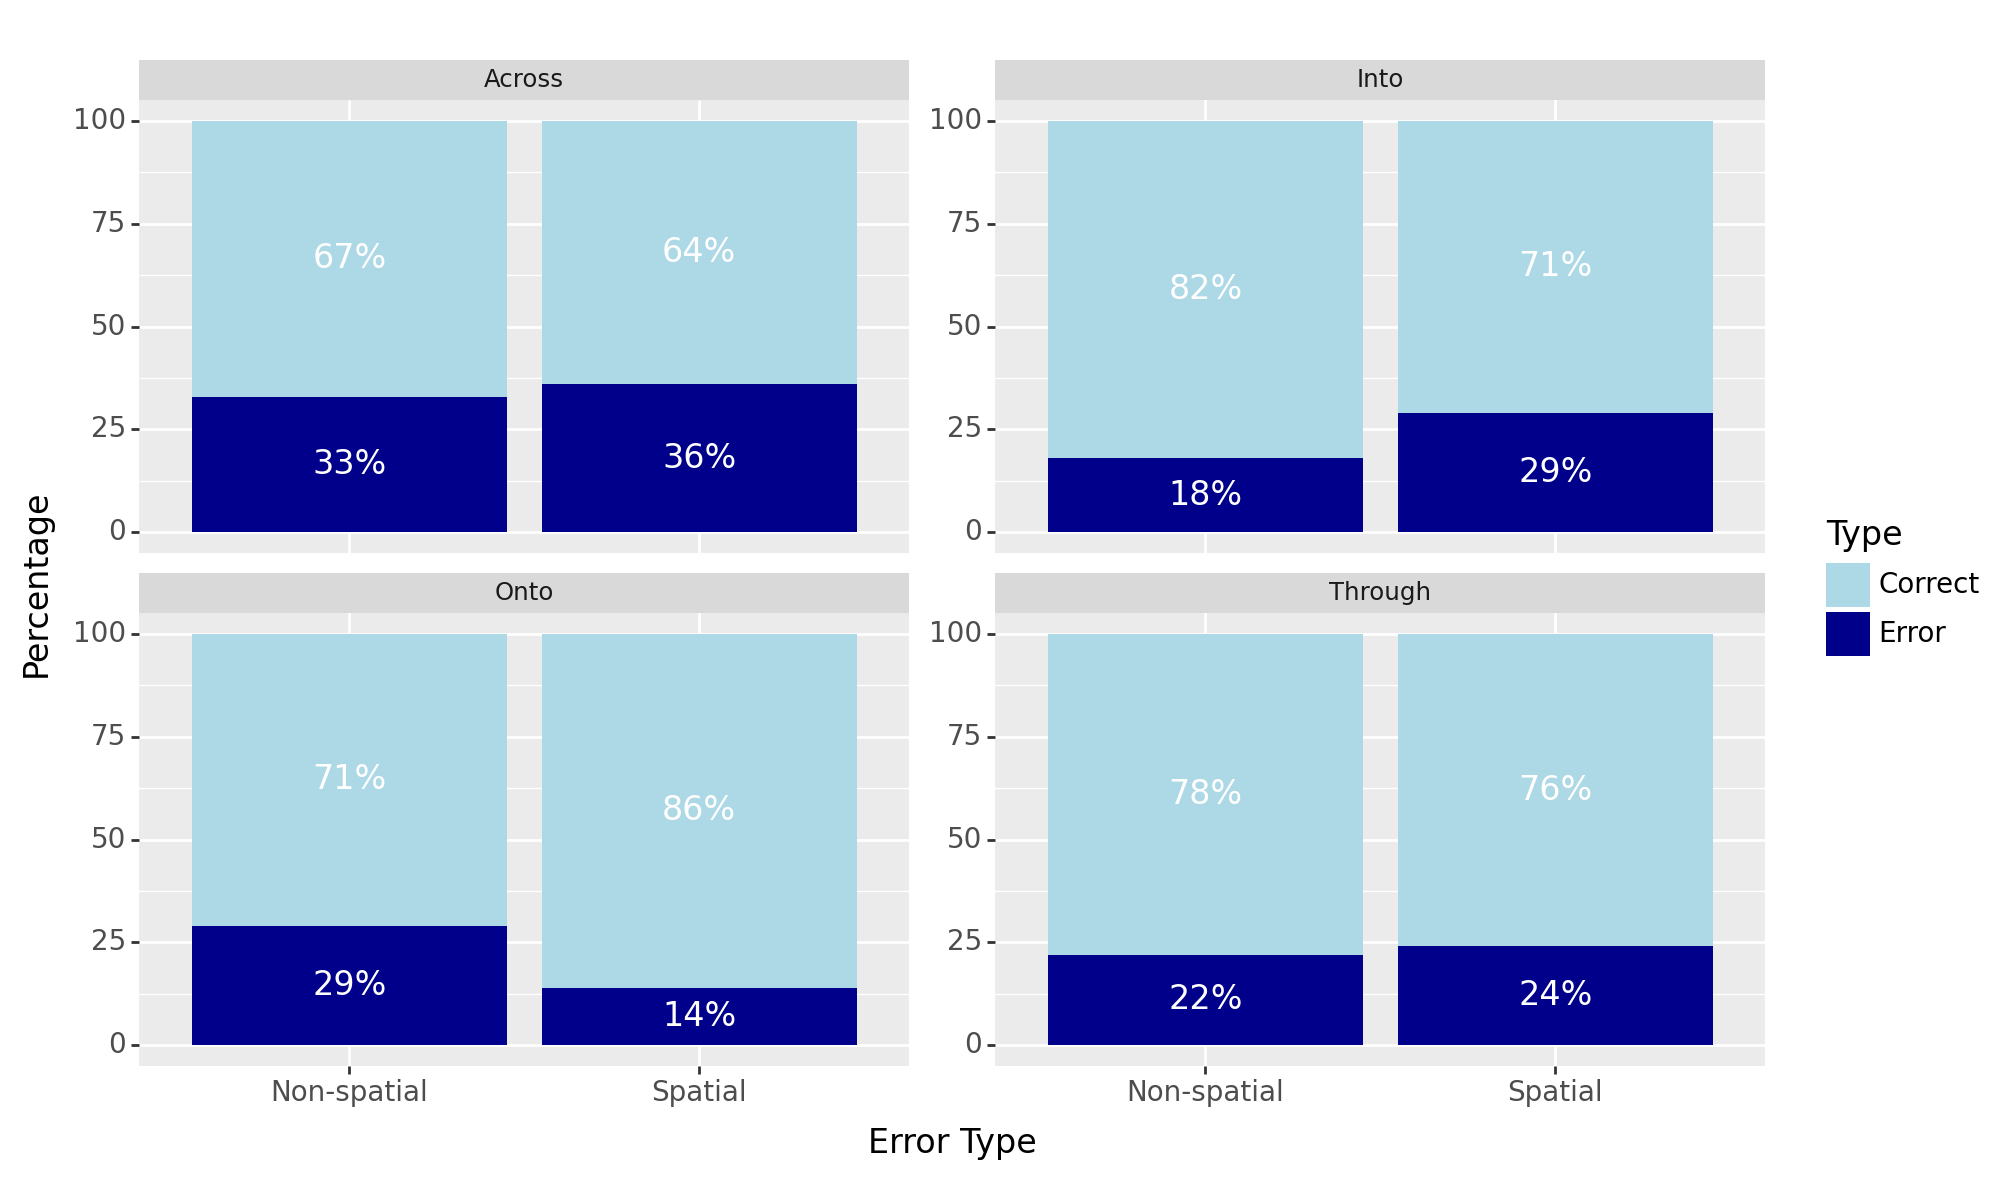
\includegraphics[width=1\textwidth]{textual/Figuras/Results/Unknown-52.png}
        \caption{Spatial vs. Non-spatial: Correct Translations and Errors by Preposition (\%).}
        \label{fig: spatial-non-perc}
\end{figure}

%We observed significant disparities in error types across preposition pairs. For instance, ACROSS was the only preposition that had considerably fewer non-spatial errors ($7$ instances, $21.9\%$ of total) but predominant spatial errors ($25$ out of $32$ instances, $78.1\%$) (See Example~\ref{ex:ex-12} for an illustration of spatial error with ACROSS). Conversely, THROUGH showcased noticeable high non-spatial errors ($73$ instances, approximately $69.5\%$ of total) and lower than half that number in spatial errors ($32$ instances, about $30.5\%$). Similarly, INTO had more prevalent non-spatial errors ($112$ instances, approximately $67.1\%$ of total) compared to spatial errors ($55$ instances, about $32.9\%$). Also, ONTO exhibited dominant non-spatial errors ($8$ instances, approximately $72.7\%$ of total) and fewer spatial errors ($3$ instances, roughly $27.3\%$) (See Example~\ref{ex:ex-13} for an illustration of non-spatial error with ONTO). 

\subsubsection{ACROSS} 

In this subsection, we analyze the occurrence count, correct count, error count, correct rate, and error rate for the preposition ACROSS, divided into non-spatial and spatial categories. The detailed statistics are presented in Table~\ref{tab:across}. The analysis reveals that, for ACROSS, the spatial category outperformed the non-spatial category in nearly all metrics: $70$ occurences vs. $21$, $45$ correct translations vs. $14$, and $25$ errors vs. $7$, with the exception of a marginal two-point difference in correct proportion ($64.28\%$ vs. $66.66\%$). Although the error rate is slightly higher for spatial ($\approx36\%$) compared to non-spatial ($\approx33\%$), we can safely affirm both categories exhibit a similar trend. This indicates that, for ACROSS, spatial and non-spatial errors may present comparable levels of difficulty, despite the first group's higher frequency. Overall, for ACROSS, spatial senses may be only slightly more prone to errors than non-spatial senses. Example~\ref{ex:ex-12} illustrates a case of spatial error with ACROSS.


\begin{table}[htb]
\centering
\begin{tabular}{lcc}
\toprule
 & \multicolumn{2}{c}{\textbf{ACROSS}} \\ 
 & \textbf{N-SP} & \textbf{SP} \\ 
\midrule
Ocurrence Count & $21$ & $70$ \\ 
Correct Count & $14$ & $45$ \\ 
Error Count & $7$ & $25$ \\ 
\midrule
Correct Rate & $\mathbf{66.66\%}$ & $64.28\%$ \\ 
\midrule
Error Rate & $33.33\%$ & $\mathbf{35.71\%}$ \\ 
\bottomrule
\end{tabular}
\caption{ACROSS: Spatial (SP) vs. Non-Spatial (N-SP): Counts and Rates.}
\label{tab:across}
\end{table}


\ex.\texttt{(inner\_id: 27316)} \hfill \texttt{Across(ii)} \\[0.3ex]
\noindent\rule{\linewidth}{0.9pt}
When I \colorbox{lightblue}{\textcolor{blue}{walked}} \colorbox{lightgray}{\textcolor{blue}{\emph{across}}} \colorbox{lightgray}{\textcolor{blue}{Afghanistan}}, I \textcolor{blue}{stayed} with people like this. (SRC) \label{ex:ex-12} \\[-0.3ex]
\noindent\rule{\linewidth}{0.3pt}
Quando \colorbox{lightgray}{\textcolor{ForestGreen}{\emph{atravessei}}} \colorbox{lightgray}{\textcolor{ForestGreen}{o Afeganistão}} \colorbox{lightblue}{\textcolor{ForestGreen}{a pé}}, \textcolor{ForestGreen}{fiquei} em casas de pessoas como esta. (REF) \\[-0.3ex]
\noindent\rule{\linewidth}{0.3pt}
?~Quando \colorbox{lightgray}{\textcolor{Maroon}{\emph{passei pela}}} \colorbox{lightgray}{\textcolor{Maroon}{Áfgão}}, \textcolor{Maroon}{passei} com pessoas como essas. (Gemma-7B) \\[-0.3ex]
\noindent\rule{\linewidth}{0.9pt}

In Example~\ref{ex:ex-12}, a spatial error involving syntactic projection (sp) is observed in the use of the preposition ACROSS. Here, the phrase ``passei pela'' incorrectly attempts to translate the spatial expression by adopting the EN lexicalization pattern of expressing motion into PT-br, a practice deemed incorrect by the literature \parencite{talmy2000towardb, slobin2005relating, McCleary-Viotti-2004}. Although the Manner element in ``walked'' is not directly translated in ``passei'' (passed), we considered this error a syntatic projection because it reflects an attempt at directly translating the EN construction. It is also worth noting that we consider the expression ``passar pelo(a) more closer in meaning with ``(go) through'' than with ``across''. Additionally, ``pela'' constitutes an agreement (ag) error, ``Áfgão'' an interlanguage/code-switching (in) error, and ``passei'' a wrong lexical choice (wl) error.


\subsubsection{$\chi^2$ Test Results for ACROSS} 

Following the analysis, the Chi-Square ($\chi^2$) Test was conducted to determine if there was a significant association between the number of errors (spatial vs. non-spatial) and correct instances in the translations. For ACROSS, the test yielded a chi-square statistic of $0.0$ (threshold is  $\chi^2 > 3.841$), a p-value of $1.0$ (threshold is  $p < 0.05$), and $1$ degree of freedom (df), indicating that the observed frequencies are very close to the expected frequencies. This result suggests no significant association between the two categories, meaning that, for this preposition, spatial and non-spatial errors do not differ significantly in their impact on overall translation accuracy. The high p-value implies that the observed distribution is entirely consistent with the null hypothesis of independence between the categories. The graph in Figure~\ref{fig: schi-across} illustrates the expected vs. observed values, highlighting this consistency and showing only slight differences such as in lower observed values in some categories.

\begin{figure}[htb]
        \centering
        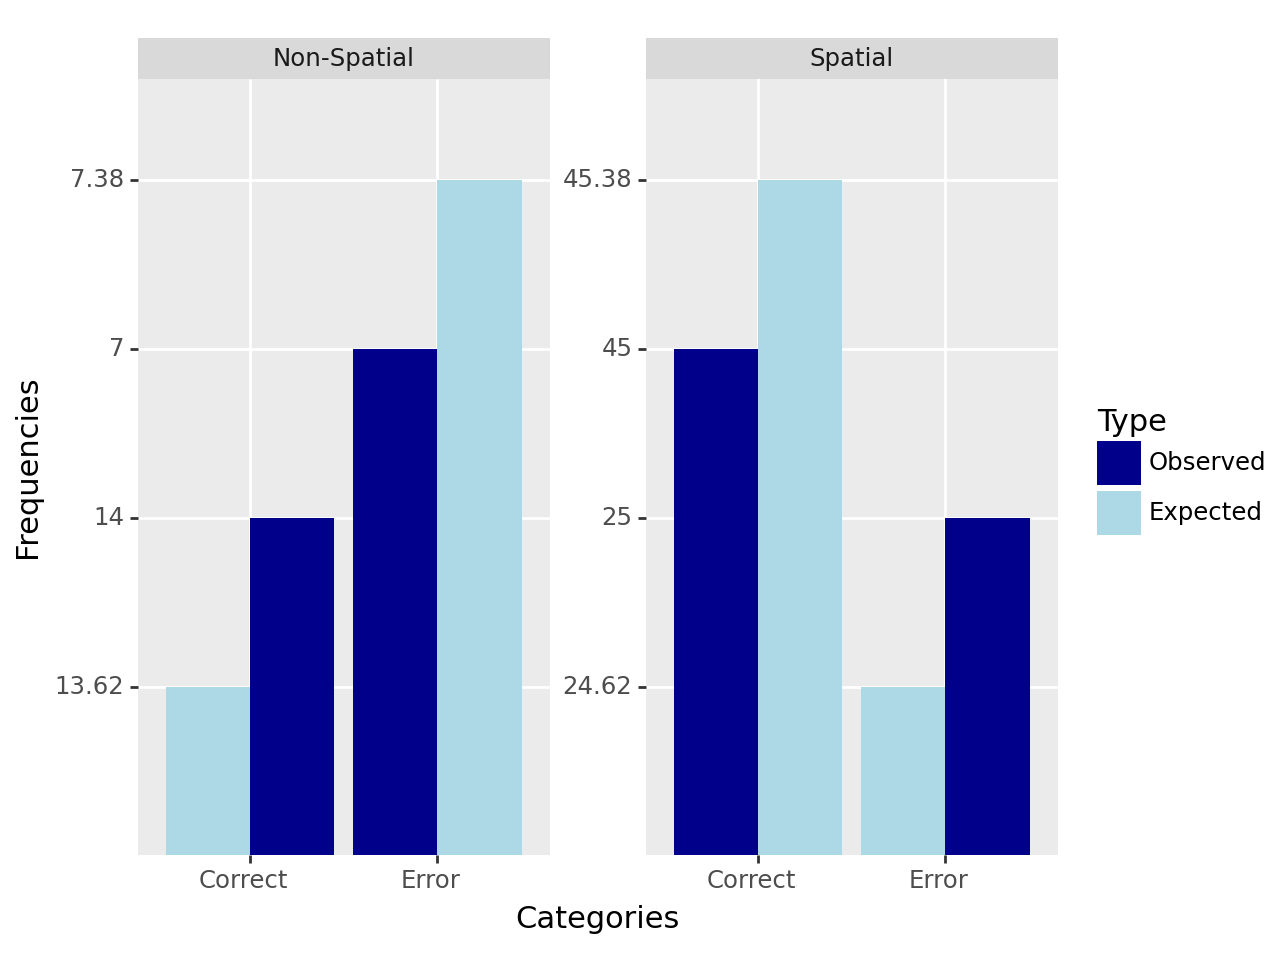
\includegraphics[width=.8\textwidth]{textual/Figuras/Results/Unknown-65.png}
        \caption{ACROSS: Observed vs. Expected Frequencies.}
        \label{fig: schi-across}
\end{figure}


\subsubsection{INTO} 

In this subsection, we provide an overview of the results for INTO. Table~\ref{tab:into} summarizes the occurrence count, correct count, error count, correct rate, and error rate obtained for INTO by category: spatial and non-spatial. The analysis reveals an interesting pattern across the statistics for the preposition INTO. While the non-spatial category presented significantly higher numbers in almost all metrics: occurrence count ($609$ vs. $189$), correct count ($497$ vs. $134$), error count ($112$ vs. $55$), and correct rate ($\approx82\%$ vs. $\approx71\%$), interestingly, its error rate was actually considerably lower ($\approx18\%$) compared to the spatial category ($\approx29\%$). This finding suggests that, while non-spatial senses were considerably more frequent for INTO, spatial senses were significantly more prone to errors, with an 11-point margin.


\begin{table}[htb]
\centering
\begin{tabular}{@{}lccc@{}} \\
\toprule
& \multicolumn{2}{c}{\textbf{INTO}} \\ 
& \textbf{N-SP} & \textbf{SP} \\
\midrule
Occurrences & $609$ & $189$\\
Correct Count  & $497$ & $134$\\
Error Count & $112$ & $55$ \\
\midrule
Correct Rate & $\mathbf{81.60\%}$ & $70.89\%$\\
\midrule
Error Rate & $18.39\%$ & $\mathbf{29.10\%}$\\
\bottomrule
\end{tabular}
\caption{INTO: Spatial (SP) vs. Non-Spatial (N-SP): Counts and Rates.} \label{tab:into} 
\end{table}


\subsubsection{$\chi^2$ Test Results for INTO} 

The analysis of the Chi-Square ($\chi^2$) Test for INTO further confirms the previous results, yielding a chi-square statistic of $9.361$ (threshold is  $\chi^2 > 3.841$), a p-value of $0.0022$ (threshold is $p < 0.05$), and $1$ degree of freedom (df). These results suggest a significant correlation between the number of errors (spatial vs. non-spatial) in translations for this preposition, rejecting the null hypothesis. This indicates that the spatial and non-spatial errors in translations for INTO are not independent and are likely influenced by some underlying factor. As can be seen in Figure~\ref{fig: schi-into}, observed frequencies deviate significantly (more than 10 points) from what would be expected if there were no association between these categories, emphasizing the strength of this correlation.

\begin{figure}[htb]
        \centering
        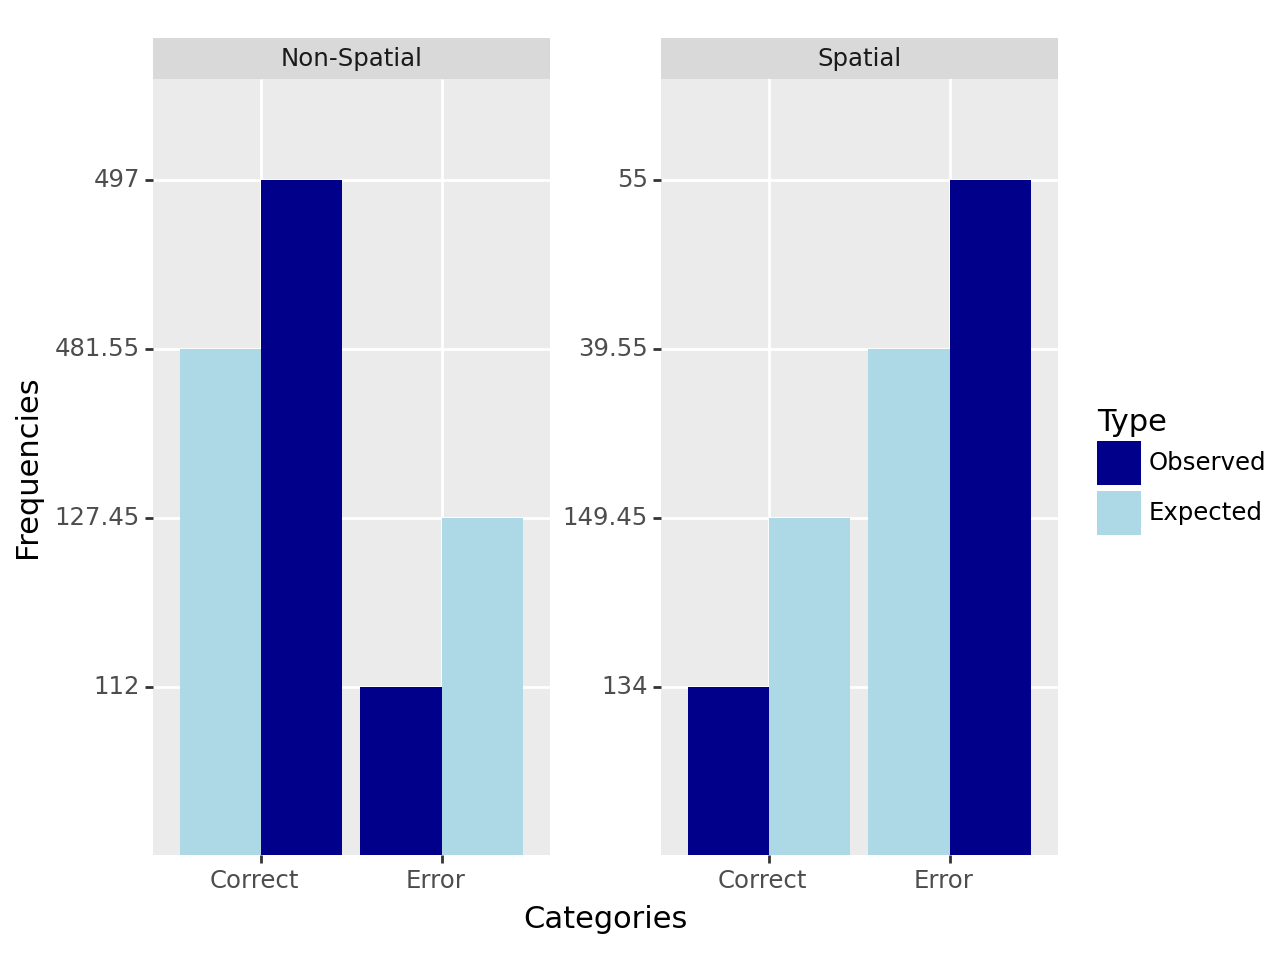
\includegraphics[width=.8\textwidth]{textual/Figuras/Results/Unknown-66.png}
        \caption{INTO: Observed vs. Expected Frequencies.}
        \label{fig: schi-into}
\end{figure}


\subsubsection{ONTO}

In this subsection, we present the results for ONTO. Table~\ref{tab:onto} displays the occurrence count, correct count, error count, correct rate, and error rate for ONTO categorized as spatial and non-spatial. The analysis reveals that non-spatial senses were slightly higher in nearly all metrics, except for error rate (with $\approx29\%$ for non-spatial compared to $\approx14\%$ for spatial senses). This second group exhibited only slightly fewer errors ($3$) compared to the first ($8$). This trend persisted across the occurrence count ($21$ vs. $28$) and correct count ($3$ vs. $8$), resulting in a lower error rate for spatial senses ($\approx14\%$) compared to non-spatial senses ($\approx29\%$). These findings suggest that non-spatial errors were marginally more frequent and presented a significantly bigger challenge than spatial errors. Example~\ref{ex:ex-13} illustrates a case with ONTO.

\begin{table}[htb]
\centering
\begin{tabular}{@{}lccc@{}} \\
\toprule
& \multicolumn{2}{c}{\textbf{ONTO}} \\ 
& \textbf{N-SP} & \textbf{SP} \\
\midrule
Occurrences & $28$ & $21$ \\
Correct Count & $20$ & $18$ \\
Error Count & $8$ & $3$ \\
\midrule
Correct Rate & $71.42\%$ & $\mathbf{85.71\%}$ \\
\midrule
Error Rate & $\mathbf{28.57\%}$ & $14.29\%$ \\
\bottomrule
\end{tabular}
\caption{ONTO: Spatial (SP) vs. Non-Spatial (N-SP) Counts and Rates.} \label{tab:onto} 
\end{table}


\ex.\texttt{(inner\_id: 32495)} \hfill \texttt{Onto(iii)} \\[0.3ex]
\noindent\rule{\linewidth}{0.9pt}
And the business organizations thought we \colorbox{lightgray}{\textcolor{blue}{were \emph{onto} something}} in terms of a way of preparing children much better for \textcolor{blue}{real-life work} today. (SRC) \label{ex:ex-13} \\[-0.3ex]
\noindent\rule{\linewidth}{0.3pt}
E as organizações empresariais acharam que \colorbox{lightgray}{\textcolor{ForestGreen}{tínhamos algo interessante}} em termos de um preparo muito melhor das crianças para \textcolor{ForestGreen}{trabalhos da vida real} dos dias de hoje. (REF) \\[-0.3ex]
\noindent\rule{\linewidth}{0.3pt}
?~E as organizações empresariais acharam que \colorbox{lightgray}{\textcolor{Maroon}{estávamos \emph{em} algo}} quando se tratava de preparar muito melhor as crianças para \textcolor{Maroon}{o trabalho real da vida} hoje. (Mixtral-8x7B) \\[-0.3ex]
\noindent\rule{\linewidth}{0.9pt}

Example~\ref{ex:ex-13} contains a case of non-spatial error involving an idiomatic expression (ie) with the preposition ONTO.  In this instance, the PT-br phrase ``estávamos em algo'' can be considered an overly-literal translation of the idiom ``(be) onto something,'' which in this context means ``having done or discovered something important, special, etc.'' according to the \textcite{merriamwebster_onto_something} dictionary. One possible way of expressing this idea in PT-br is ``tínhamos algo interessante,'' such as in the reference (REF). Furthermore, ``o trabalho REAL da vida'' constitutes an interesting case of grammar/orthography (gr) error involving incorrect word order, which, in this case, completely changed the original meaning of ``trabalho da vida REAL'' (real-life work).


\subsubsection{$\chi^2$ Test Results for ONTO} 

The analysis of the Chi-Square ($\chi^2$) Test for ONTO yielded a chi-square statistic of $0.706$ (threshold is  $\chi^2 > 3.841$), a p-value of $0.401$ (threshold is  $p < 0.05$), and $1$ degree of freedom (df). These results indicate that there is no significant correlation between the number of errors (spatial vs. non-spatial) in translations for the ONTO preposition, as the p-value exceeds the typical significance level of $0.05$. The expected frequencies, as illustrated in Figure~\ref{fig: schi-onto}, further support this conclusion, with observed frequencies closely aligning (less than 2 points) with what would be expected under the null hypothesis of independence between the categories.

\begin{figure}[htb]
        \centering
        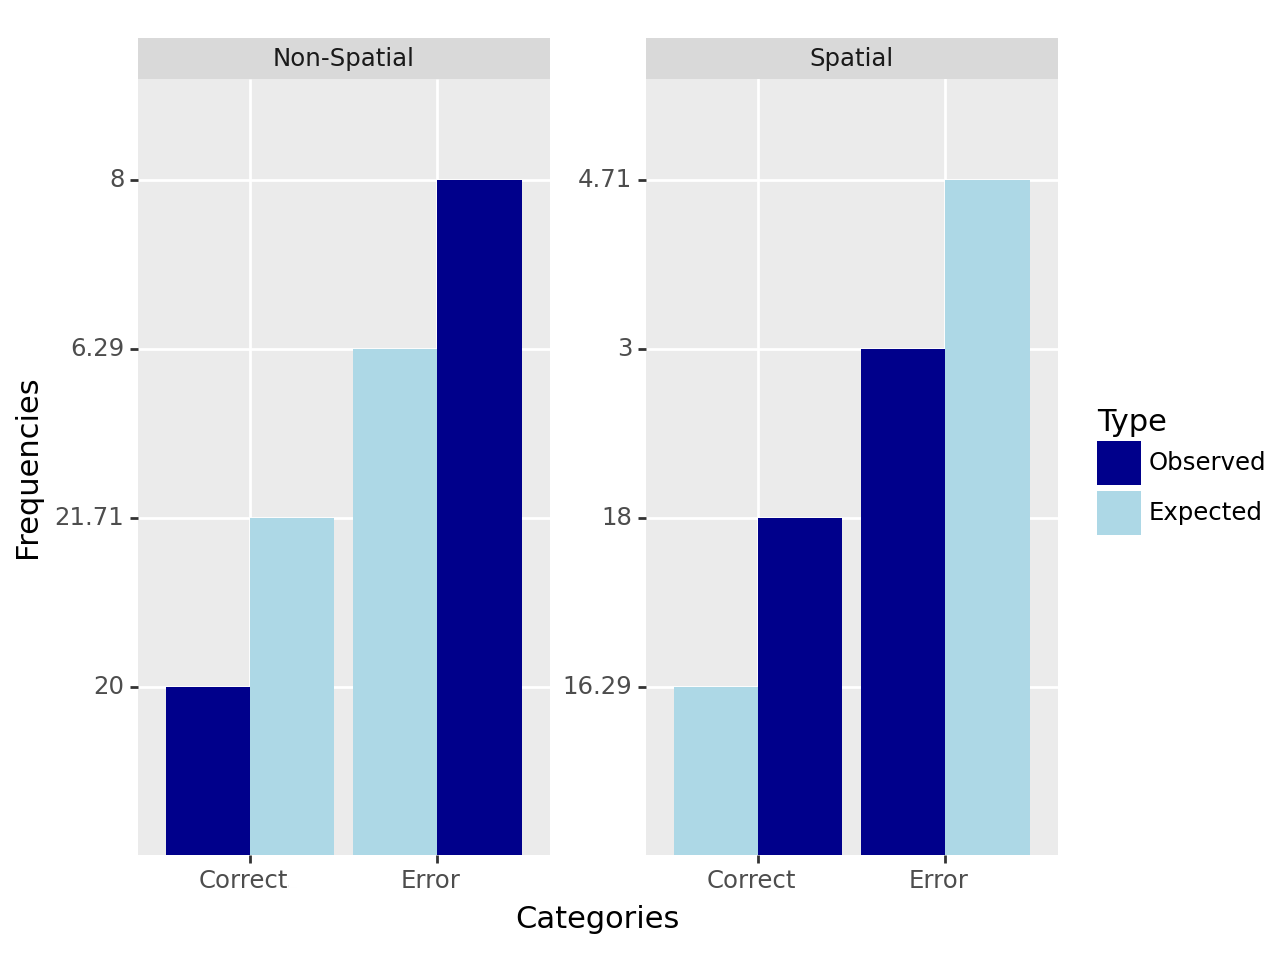
\includegraphics[width=.8\textwidth]{textual/Figuras/Results/Unknown-67.png}
        \caption{ONTO: Observed vs. Expected Frequencies.}
        \label{fig: schi-onto}
\end{figure}


\subsubsection{THROUGH}

Table~\ref{tab:through} provides a summary of the occurrences, correct count, error count, correct rate, and error rate associated with the preposition THROUGH, categorized as spatial and non-spatial. The analysis indicates that non-spatial senses exhibited a considerably higher number of occurrences ($336$) compared to spatial senses ($133$), as well as correct count ($263$ vs. $101$), error count ($73$ vs. $32$), resulting in a slightly higher correct rate ($\approx79\%$ vs. $\approx76\%$). However, despite these higher numbers, we observe a slightly lower error rate for this category ($\approx22\%$) compared to spatial senses ($\approx24\%$). This suggests that, while non-spatial senses were more prevalent, spatial senses had a slightly higher error proportion, indicating an almost comparable challenge in their accurate usage.

\begin{table}[htb]
\centering
\begin{tabular}{@{}lccc@{}} \\
\toprule
& \multicolumn{2}{c}{\textbf{THROUGH}} \\ 
& \textbf{SP} & \textbf{N-SP} \\
Occurrences & $133$ & $336$ \\
Correct Count & $101$  & $263$\\
Error Count & $32$ & $73$ \\
\midrule
Correct Rate & $75.93\%$ & $\mathbf{78.72\%}$ \\
\midrule
Error Rate & $\mathbf{24.06\%}$ & $21.73\%$ \\
\bottomrule
\end{tabular}
\caption{THROUGH: Spatial (SP) vs. Non-spatial (N-SP) Counts and Rates.} \label{tab:through} 
\end{table}

\subsubsection{$\chi^2$ Test Results for THROUGH} 

The Chi-Square ($\chi^2$) Test conducted for the preposition THROUGH resulted in a chi-square statistic of $0.179$ (threshold is $\chi^2 > 3.841$), with a corresponding p-value of $0.672$ (threshold is $p < 0.05$) and $1$ degree of freedom (df). These findings suggest that there is no significant correlation between the number of errors (spatial vs. non-spatial) in translations for this preposition, as the p-value far exceeds the conventional significance level of $0.05$. Moreover, as illustrated in Figure~\ref{fig: through-chi}, the observed frequencies closely match the expected frequencies (with less than 3 points) under the assumption of independence between the categories. Thus, the data does not provide sufficient evidence to reject the null hypothesis of independence.

\begin{figure}[htb]
        \centering
        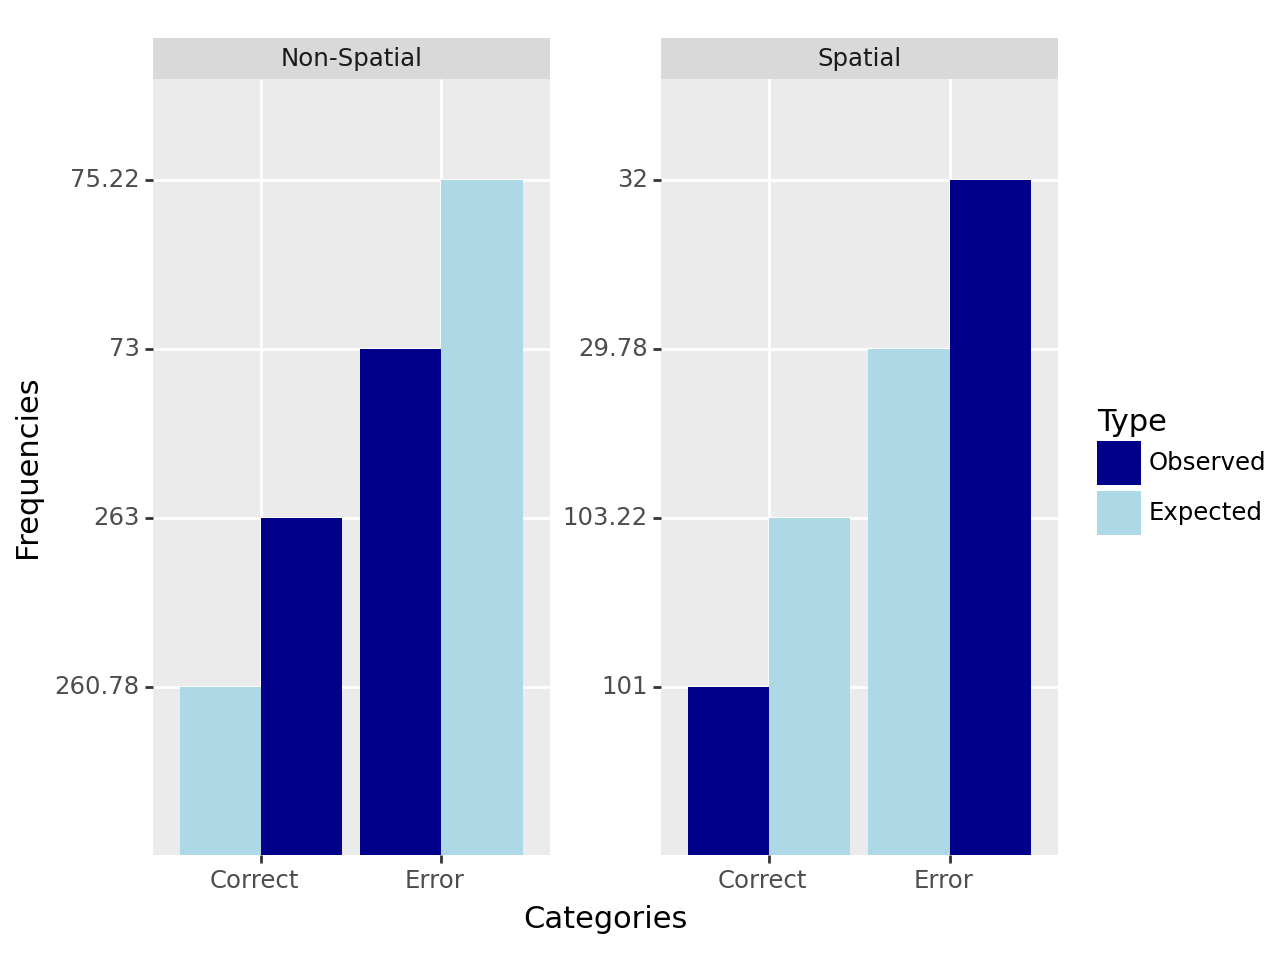
\includegraphics[width=.7\textwidth]{textual/Figuras/Results/Unknown-68.png}
        \caption{THROUGH: Observed vs. Expected Frequencies.}
        \label{fig: through-chi}
\end{figure}


%Based on our findings, we hypothesize whether the frequency of a given preposition in real-world scenarios could potentially impact the errors observed in our analysis. We noted that spatial errors were more common for prepositions that are less frequent in idioms and phrasal verbs, such as ACROSS. This suggests that, in this case, translating spatial relationships may pose greater challenges. Conversely, we observed significant variation in non-spatial error prevalence for INTO, indicating that there may be nuanced difficulties in translating idiomatic expressions. One potential explanation, we thought, might be the higher occurrence of phrasal verbs and idioms containing INTO compared to ACROSS, which could contribute to models' struggles with non-spatial errors.

%To confirm our premise, we compiled a list of phrasal verbs from \texttt{Wiktionary}\footnote{\href{https://en.wiktionary.org/wiki/Wiktionary:Main\_Page}{https://en.wiktionary.org/wiki/Wiktionary:Main\_Page}} by Wikipedia using JSON data and then filtered them by preposition to ascertain their incidence for each of the four prepositions we analyzed. The results are summarized in Table~\ref{tab:prevalence}. For the complete lists of phrasal verbs, please refer to the Attachments Section (Tables~\ref{a:across} (for ACROSS), \ref{a:into} (for INTO), \ref{a:onto} (for ONTO), \ref{a:through} (for THROUGH)).

%\begin{table}[ht]
%\centering
%\begin{tabular}{@{}lcc@{}} \\
%\midrule
%\toprule
%\textbf{Preposition} & \textbf{N. of Phrasal Verbs} \\
%\midrule
%Across  & $11$ \\
%Into & \colorbox{lightgray}{$61$} \\
%%%%Onto & $11$ \\
%%%Through & \colorbox{lightgray}{$60$} \\
%%\bottomrule
%\midrule
%\end{tabular}
%\caption{Prevalence of Prepositions in Phrasal Verbs (Source: Wiktionary by Wikipedia).} \label{tab:prevalence} 
%\end{table}

%These findings confirm that the prevalence of spatial prepositions in EN phrasal verbs varies considerably. We observed a potential correlation between the frequency of phrasal verbs and the distribution of non-spatial errors. For instance, prepositions like INTO and THROUGH, which have more phrasal verbs, showed a greater prevalence of non-spatial errors, indicating that their complexity may affect the models' performance. On the other hand, the lower occurrence of ONTO phrasal verbs may explain its relatively lower non-spatial counts, and, possibly, its low spatial error rate. Overall, this analysis suggests that ACROSS and ONTO may be less frequently used in real-world spatial descriptions, and since the realm of idiomatic expressions is an extension of the spatial domain, as described by Cogitive Theorists like ~\textcite{LakoffJohnson80, coventry:04b}, this could make them less common in non-spatial description as well.

%Overall, these insights highlight the complexity of EN idiomatic expression usage and its impact on NMT. Understanding the relationship between the use of spatial prepositions in phrasal verbs and error distribution can guide the development of targeted strategies to enhance the quality of NMT systems.

\subsection{Analysis by Meaning: Spatial vs. Non Spatial Errors}
\label{subsec: sp-vs-nsp}

This analysis extends the previous investigation. Our main goal was to identify which specific meanings associated with each preposition (please refer back to Table~\ref{tab:prep-categorizations} for the complete list) most adversely impacted the translations. We were particularly interested in discovering which spatial meanings of ACROSS, THROUGH, INTO, and ONTO, as defined by \textcite{bruckfield2011prepositions}, significantly influenced the quality of the translations.

We used the same two distinct groups of errors from the previous analysis: ``Spatial,'' consisting of polysemy (po), syntactic projection (sp), and wrong sense (ws) errors, and ``Non-spatial,'' consisting of idiomatic expression (ie) errors. Figure~\ref{fig: all-perc} offers an overview of the distribution of correct translations and errors for each preposition by meaning. Table~\ref{tab:combined}, in Attachment~\ref{att2}, provides an overview of the occurrence count, correct count, error count, correct rate, and error rate for the two groups.

\begin{figure}[htb]
        \centering
        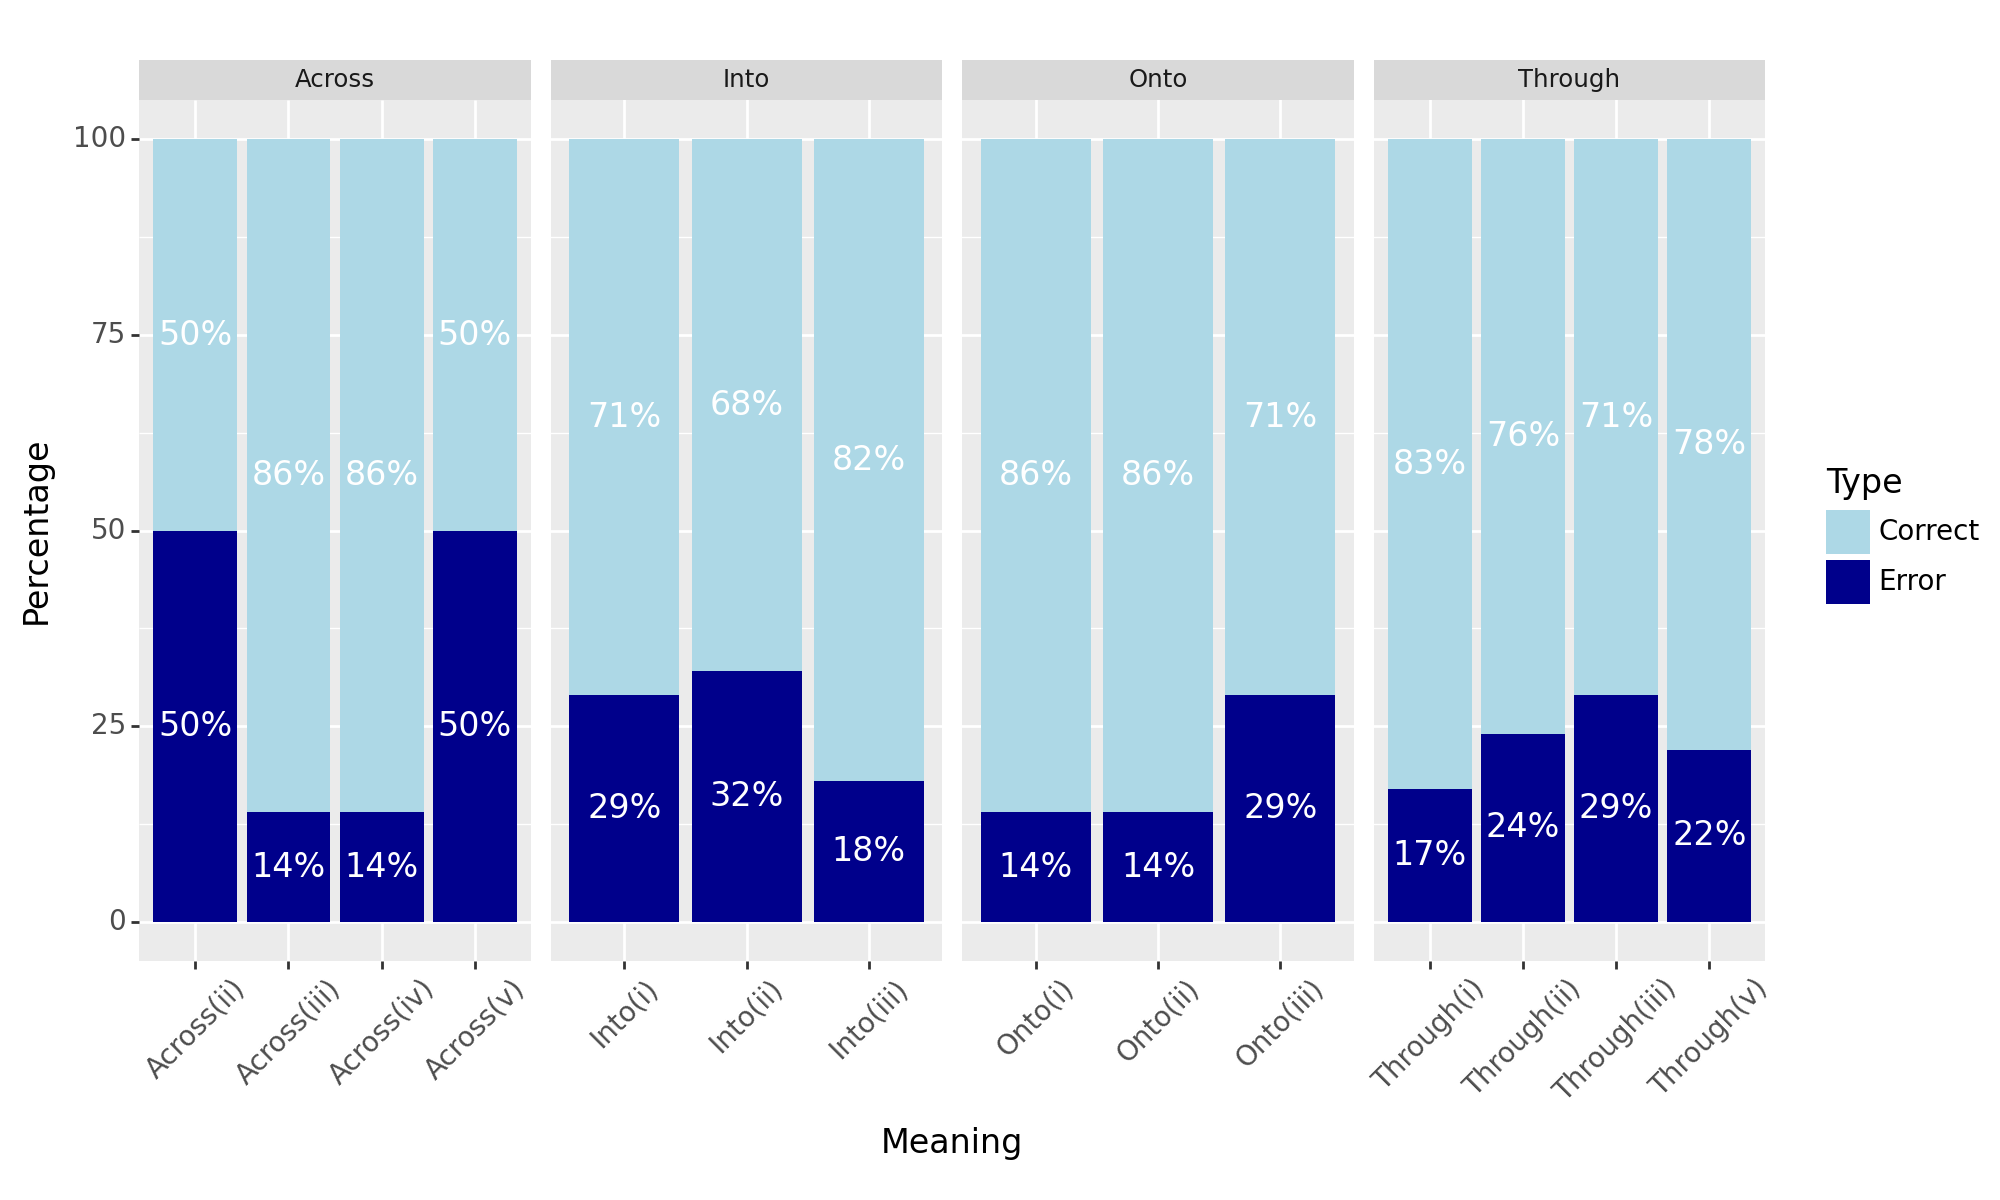
\includegraphics[width=1\textwidth]{textual/Figuras/Results/Unknown-71.png}
        \caption{ACROSS, INTO, ONTO, and THROUGH: Correct and Error Rates by Meaning (\%).}
        \label{fig: all-perc}
\end{figure}

\subsubsection{ACROSS by Meaning}

In this subsection, we present the number of occurrences, correct count, error count, correct rate, and error rate for ACROSS by meaning. Table~\ref{tab:across-senses} displays these statistics. 

The results reveal significant variations in the performance of models across different meanings of ACROSS. For spatial meanings, both ``Across(iii) -- Opposite location'' and ``Across(iv) -- Distribution'' exhibit the highest correct proportions, each at $\approx86\%$. Conversely, the non-spatial meaning ``Across(v)'' and ``Across(ii) -- Movement over a surface'' show lower correct rates, both at $50\%$. Notably, the error rates mirror this trend, with ``Across(ii)'' and ``Across(v)'' having the highest error rates at $50\%$, indicating these meanings presented more challenges for accurate translation. These rates underscore the models' strengths in handling specific spatial contexts while highlighting the need for improvement in non-spatial and ``Across(ii)'' contexts.


\begin{table}[htb]
\centering
\begin{tabular}{lcccc}
\toprule
 & \multicolumn{4}{c}{\textbf{ACROSS by Meaning}} \\ 
 & \multicolumn{3}{c}{\textbf{SP}} & \textbf{N-SP} \\ 
 & Across(ii) & Across(iii) & Across(iv) & Across(v) \\
\midrule
Occurrences & $42$ & $7$ & $21$ & $14$ \\
Correct Count & $21$ & $6$ & $18$ & $7$ \\ 
Error Count & $21$ & $1$ & $3$ & $7$ \\ 
\midrule
Correct Rate & $50.00\%$ & $\mathbf{85.71\%}$ & $\mathbf{85.71\%}$ & $50.00\%$ \\ 
\midrule
Error Rate & $\mathbf{50.00\%}$ & $14.28\%$ & $14.28\%$ & $\mathbf{50.00\%}$ \\ 
\bottomrule
\end{tabular}
\caption{ACROSS: Spatial (SP) vs. Non-spatial (N-SP) Counts and Rates by Meaning.}
\label{tab:across-senses}
\end{table}


\subsubsection{$\chi^2$ Test Results for ACROSS by Meaning} 

The Chi-square analysis of the data from Table~\ref{tab:across-senses} reveals a Chi-square statistic of $10.10$  (threshold is $\chi^2 > 7.815$) with a p-value of $0.018$ (threshold is $p < 0.05$) and $3$ degrees of freedom (df) of. The difference between expected and observed frequencies for the correct and error counts across the different meanings of ACROSS are illustrated in Figure~\ref{fig:across-senses-chi}. The p-value of $0.018$, being less than the typical significance level of $0.05$, indicates that there is a statistically significant difference in the distribution of correct and error counts across the different meanings of ACROSS. This suggests that the models do not perform equally across all meanings, highlighting specific areas where the models struggle, particularly with the non-spatial meaning and the "Movement over a surface" meaning. This underscores the necessity for further refinement in handling these contexts.

\begin{figure}[htb]
        \centering
        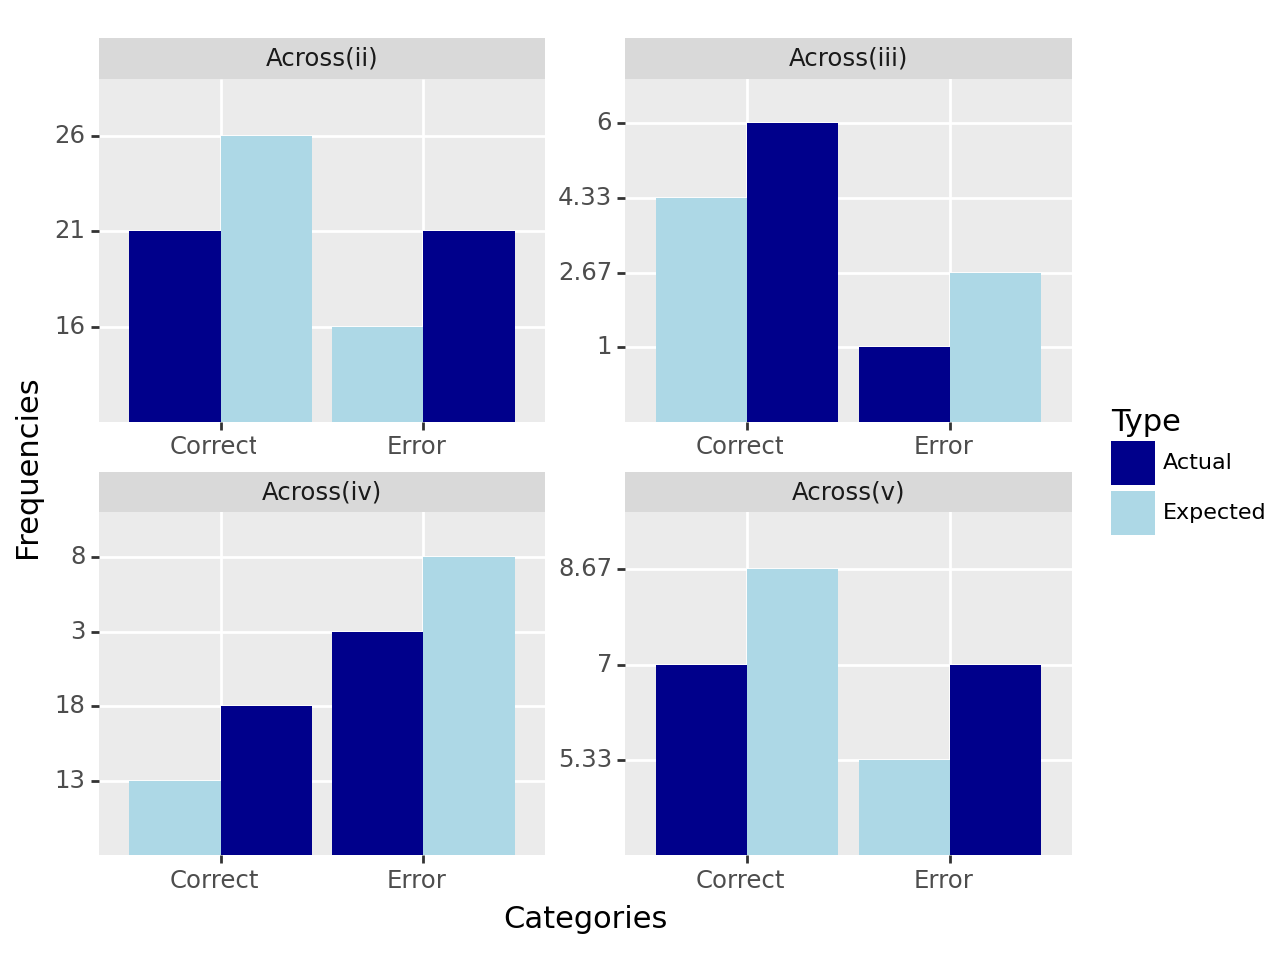
\includegraphics[width=.8\textwidth]{textual/Figuras/Results/Unknown-70.png}
        \caption{ACROSS: Observed vs. Expected Frequencies by Meaning.}
        \label{fig:across-senses-chi}
\end{figure}


%Once again, we observed significant disparities in the occurrences of errors caused by the different preposition senses. For instance, out of the $25$ spatial errors identified for ACROSS, $21$ are associated with the sense Across(2), which indicates ``movement over a surface'', " comprising a surprising $65\%$ of instances. The second largest group was Across(5), which is when the preposition is ``non-spatial'', with $21.9\%$ ($7$ errors). The remaining spatial senses, Across(4), ``distribution'' and Across(3), ``opposite location'', together comprise $12.5\%$ (with $4$ errors in total). Conversely, for INTO, the sense Into(1) ``movement leading to enclosure'' had the highest number of spatial errors, with $46$ ($27.5\%$), followed by Into(2), which indicates ``movement resulting in collision,'' with $9$ errors ($5.4\%$). The highest proportion of errors ($67\%$) was still observed in the sense Into(3), denoting ``non-spatial'' use, with a massive $112$ errors. THROUGH had similar behavior, with the majority of errors ($73$, or $69.5\%$) connected to the ``non-spatial'' sense THROUGH(5). Out of the $32$ spatial errors, $19.0\%$ are connected to sense THROUGH(3) ``movement past a barrier,'' $6.7\%$ are connected to ``movement within a passage/conduit'', THROUGH (1), and $4.8\%$ are connected to ``movement within an open area'', THROUGH(2), with $20$, $7$, and $5$ errors, respectively. And lastly, ONTO, which showed the smallest number of occurences, had $8$ ``non-spatial'' errors (sense ONTO(3)) and a total of $3$ spatial erros, with senses ONTO(1), ``movement to a surface'', comprising $18.2\%$ and ONTO(2), ``sense of attachment'', comprising $9.1\%$ \parencite{bruckfield2011prepositions, cambridge-across, cambridge-into, cambridge-onto, cambridge-through}. For your information, senses ACROSS(1), ``perpendicular position'' and THROUGH(4), ``part of a route'' were not identified in the sample for human review.

\subsubsection{INTO by Meaning}

This subsection presents the number of occurrences, correct count, error count, correct rate, and error rate for each meaning of INTO. Table~\ref{tab:into-senses} displays this statistics.  The results illustrate varying performance across different senses of INTO. The non-spatial meaning ``Into(iii)'' shows the highest correct rate at $\approx82\%$, indicating strong translation capabilities. Conversely, spatial meanings ``Into(i)'' and ``Into(ii)'' exhibit slightly lower correct proportions at $\approx71\%$ and $\approx68\%$, respectively. Error proportions reveal challenges in translating spatial meanings, with ``Into(ii)'' showing the highest error rate at $\approx32\%$. In contrast, the non-spatial meaning ``Into(iii)'' has a lower error rate at $\approx18\%$, suggesting better performance. These findings underscore the models' varying proficiency across different senses of INTO, with potential implications for improving translation accuracy, particularly in spatial contexts such as ``Movement or direction leading to enclosure'' and ``Movement resulting in physical contact or collision.''


\begin{table}[htb]
\centering
\begin{tabular}{lccc}
\toprule
 & \multicolumn{3}{c}{\textbf{INTO by Meaning}} \\ 
 & \multicolumn{2}{c}{\textbf{SP}} & \textbf{N-SP} \\ 
 & Into(i) & Into(ii) & Into(iii) \\
\midrule
Occurrences & $161$ & $28$ & $609$ \\ 
Correct Count & $115$ & $19$ & $497$ \\ 
Error Count & $46$ & $9$ & $112$ \\ 
\midrule
Correct Rate & $\mathbf{71.42\%}$ & $67.85\%$ & $\mathbf{81.60\%}$ \\
\midrule
Error Rate & $28.57\%$ & $\mathbf{32.14\%}$ & $18.39\%$
\\ 
\bottomrule
\end{tabular}
\caption{INTO: Spatial (SP) vs. Non-Spatial (N-SP) Counts and Rates by Meaning.}
\label{tab:into-senses}
\end{table}


\subsubsection{$\chi^2$ Test Results for INTO by Meaning} 

The Chi-square examination of the data from Table~\ref{tab:into-senses} resulted in a Chi-square value of $10.18$ (threshold is $\chi^2 > 5.991$), accompanied by a p-value of $0.006$ (threshold is $p < 0.05$) and degrees of freedom (df) of $2$. The disparity between expected and observed frequencies across the distinct meanings of INTO is depicted in Figure~\ref{fig: into-mean-chi}. With a p-value of $0.006$, notably lower than the standard significance level of $0.05$, the analysis underscores a statistically notable distinction in the distribution of accurate and erroneous counts among the various interpretations of INTO. This disparity suggests divergent performance among models across these interpretations, pinpointing specific domains that may benefit from refinement, particularly in spatial translation contexts.

\begin{figure}[htb]
        \centering
        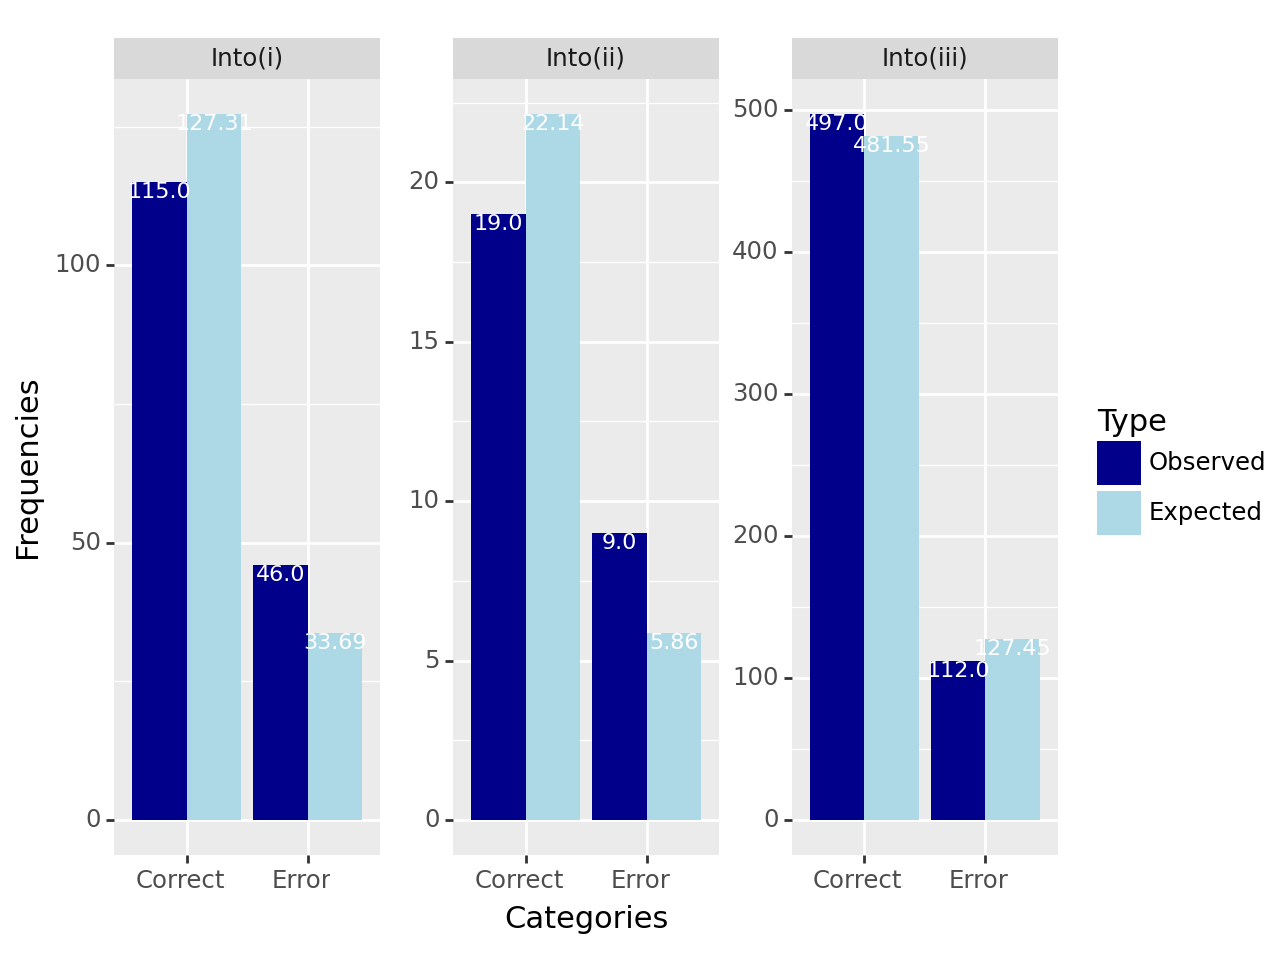
\includegraphics[width=.8\textwidth]{textual/Figuras/Results/Unknown-81.png}
        \caption{INTO: Observed vs. Expected Frequencies by Meaning (\%).}
        \label{fig: into-mean-chi}
\end{figure}

\subsubsection{ONTO by Meaning}

Table~\ref{tab:onto-mean} presents an analysis of translation performance across different meanings of ONTO. In spatial contexts, both ``Onto(i) -- Movement to a location on a surface'' and ``Onto(ii) -- Sense of attachment'' exhibit high correct rates, each at $\approx86\%$. This indicates strong translation accuracy for these spatial meanings. Conversely, the non-spatial meaning ``Onto(iii)'' demonstrates a lower correct proportion at $\approx71\%$, suggesting comparatively more challenges in accurately translating non-spatial contexts. When considering error rates, both spatial meanings ``Onto(i)'' and ``Onto(ii)'' show similar error proportions of $\approx14\%$, while the non-spatial meaning ``Onto(iii)'' has the highest error rate at $\approx29\%$. These findings highlight the models' effectiveness in handling spatial senses, emphasizing areas for improvement in accurately translating non-spatial meanings, particularly in the context of ``Sense of attachment.''

\begin{table}[htb]
\centering
\begin{tabular}{lccc}
\toprule
 & \multicolumn{3}{c}{\textbf{ONTO by Meaning}} \\ 
 & \multicolumn{2}{c}{\textbf{SP}} & \textbf{N-SP} \\ 
 & Onto(i) & Onto(ii) & Onto(iii) \\
\midrule
Occurrences & $14$ & $7$ & $28$ \\ 
Correct Count & $12$ & $6$ & $20$ \\ 
Error Count & $2$ & $1$ & $8$ \\ 
\midrule
Correct Rate & $\mathbf{85.71\%}$ & $\mathbf{85.71\%}$ & $71.42\%$ \\ 
\midrule
Error Rate & $14.28\%$ & $14.28\%$ & $\mathbf{28.57\%}$ \\ 
\bottomrule
\end{tabular}
\caption{ONTO: Spatial (SP) vs. Non-spatial (N-SP) Counts and Rates by Meaning.}
\label{tab:onto-mean}
\end{table}

\subsubsection{$\chi^2$ Test Results for ONTO by Meaning} 

The Chi-square analysis conducted on the data from Table~\ref{tab:onto-mean} yielded a Chi-square statistic of $0.176$ (threshold is $\chi^2 > 5.991$) with a p-value of $0.916$ and $2$ degrees of freedom (df). Figure~\ref{fig: onto-mean-chi} illustrates the disparities between expected and observed frequencies for the correct and error counts across the different meanings of ONTO. With a p-value of $0.916$, significantly higher than the typical significance level of $p < 0.05$, the analysis indicates no statistically significant difference in the distribution of correct and error counts across the various senses of ONTO. This suggests that, probably due to the limited data for ONTO, models performed similarly across these senses, regardless of the spatial or non-spatial context.

\begin{figure}[htb]
        \centering
        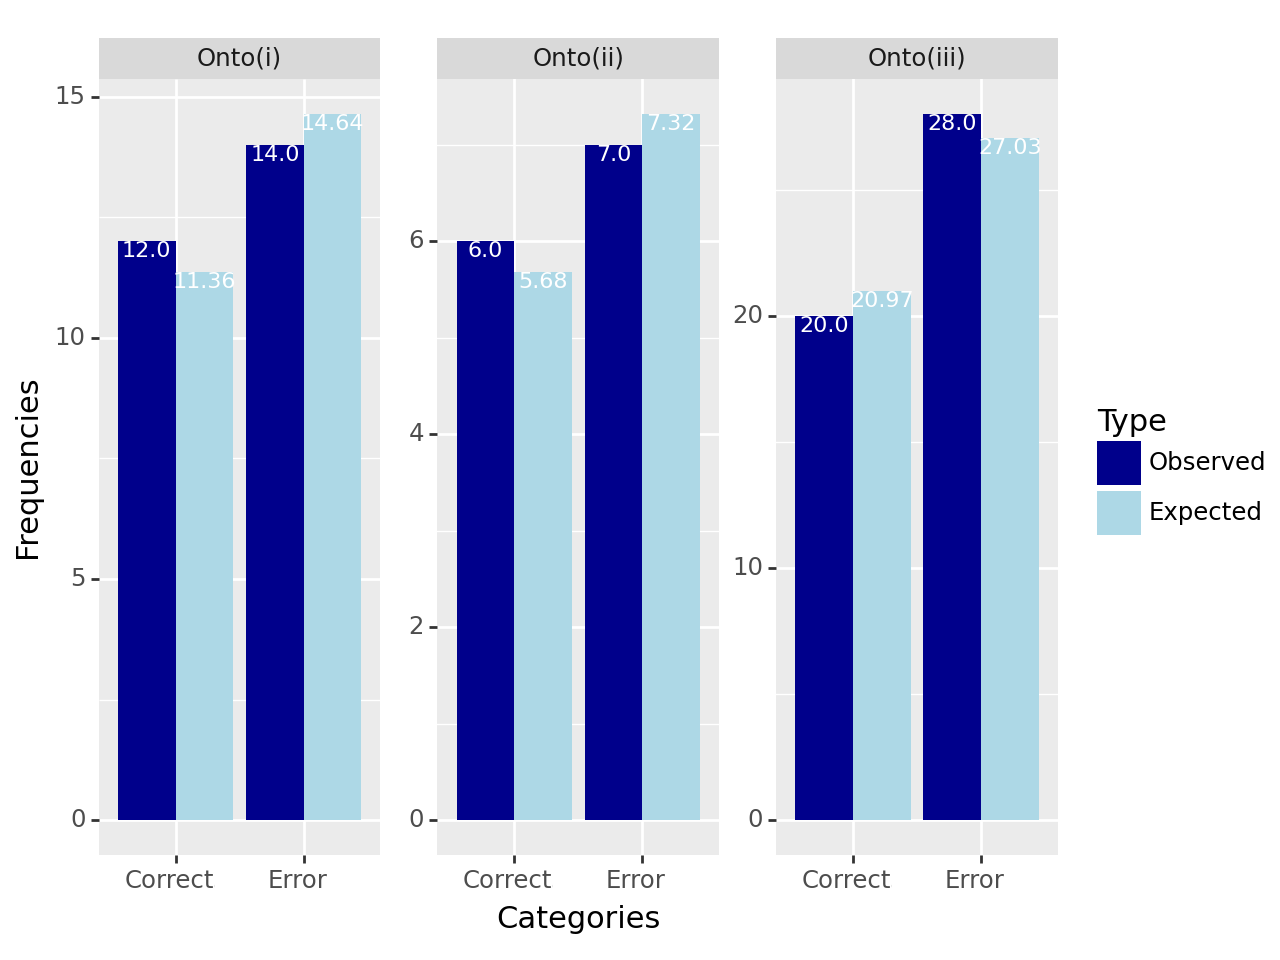
\includegraphics[width=.7\textwidth]{textual/Figuras/Results/Unknown-78.png}
        \caption{ONTO: Observed vs. Expected Frequencies by Meaning (\%).}
        \label{fig: onto-mean-chi}
\end{figure}

\subsubsection{THROUGH by Meaning}

This subsection presents the number of occurrences, correct count, error count, correct rate, and error rate for each meaning of THROUGH. Table~\ref{tab:into-senses} displays this statistics. 

\begin{table}[htb]
\centering
\begin{tabular}{lcccc}
\toprule
 & \multicolumn{4}{c}{\textbf{THROUGH by Meaning}} \\ 
 & \multicolumn{3}{c}{\textbf{SP}} & \textbf{N-SP} \\ 
 & Through(i) & Through(ii) & Through(iii) & Through(v) \\
\midrule
Occurrences & $42$ & $21$ & $70$ & $336$ \\ 
Correct Count & $35$ & $16$ & $50$ & $263$ \\  
Error Count & $7$ & $5$ & $20$ & $73$ \\ 
\midrule
Correct Rate & $\mathbf{83.33\%}$ & $76.19\%$ & $71.42\%$ & $78.27\%$ \\ 
\midrule
Error Rate & $16.66\%$ & $23.80\%$ & $\mathbf{28.57\%}$ & $21.72\%$ \\ 
\bottomrule
\end{tabular}
\caption{THROUGH: Spatial (SP) vs. Non-spatial (N-SP) Counts and Rates by Meaning.}
\label{tab:through-senses}
\end{table}

The analysis of the data in Table~\ref{tab:through-senses} reveals different model performance across the meanings of THROUGH. The highest correct rate, $\approx83\%$, is for ``Through(i)'' which represents ``movement within a passage or conduit''. This suggests that models are particularly accurate in contexts involving clear pathways or conduits. Conversely, the highest error rate, $\approx29\%$, occurs for ``Through(iii),'' which denotes ``movement past or penetrating a barrier'', indicating that models struggle most with scenarios involving this meaning. The ``Through(v)'' category, representing non-spatial usage, shows a correct rate of $\approx78\%$ and an error rate of $\approx22\%$, reflecting moderate accuracy. Overall, the performance varies significantly by meaning, with spatial contexts involving passages being easier for models than those involving barriers.

\subsubsection{$\chi^2$ Test Results for THROUGH by Meaning} 

The Chi-square analysis of the data from Table~\ref{tab:through-senses} yielded a Chi-square statistic of $2.44$ (threshold is $\chi^2 > 7.815$) with a p-value of $0.49$ (threshold is $p < 0.05$) and $3$ degrees of freedom (df). Figure~\ref{fig:through-mean-chi} illustrates the disparities between expected and observed frequencies for the correct and error counts across the different meanings of THROUGH. This indicates that there is no statistically significant difference in the distribution of correct and error counts across the various senses of THROUGH. The high p-value suggests that the observed variation in model performance across different meanings of THROUGH is not statistically significant. Therefore, the differences in correct and error rates do not imply a meaningful disparity in model performance across spatial and non-spatial contexts. This suggests that models perform similarly across these senses, regardless of the specific spatial or non-spatial context.

\begin{figure}[ht]
        \centering
        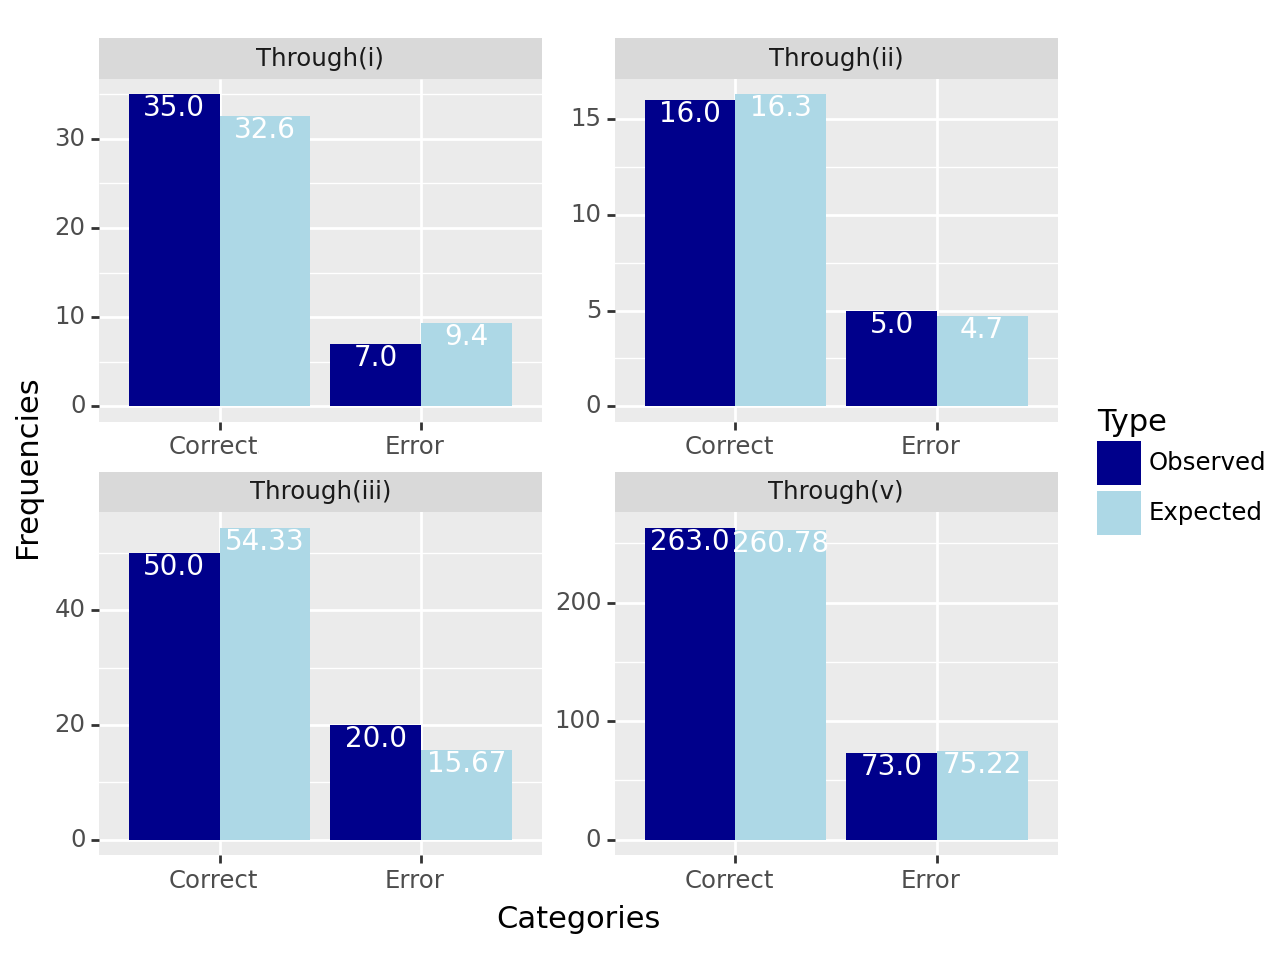
\includegraphics[width=.8\textwidth]{textual/Figuras/Results/Unknown-79.png}
        \caption{THROUGH: Observed vs. Expected Frequencies by Meaning (\%)}
        \label{fig:through-mean-chi}
\end{figure}

\subsubsection{TOTAL} 

In this subsection, we provide the results for the number of occurrences, correct count, error count, correct rate, and error rate across all prepositions. Table~\ref{tab:total} displays the statistics for both spatial and non-spatial categories.

\begin{table}[htb]
\centering
\begin{tabular}{@{}lccc@{}} \\
\toprule
& \multicolumn{2}{c}{\textbf{TOTAL}} \\ 
& \textbf{SP} & \textbf{N-SP} \\
\midrule
Occurrences & $413$ & $987$ \\
Correct Count & $298$ & $787$ \\
Error Count & $115$ & $200$ \\
\midrule
Correct Rate & $72.15\%$ & $\mathbf{79.73\%}$ \\
\midrule
Error Rate & $\mathbf{27.84\%}$ & $20.26\%$ \\
\bottomrule
\end{tabular}
\caption{TOTAL: Spatial (SP) vs. Non-Spatial (N-SP) Observed vs. Expected Frequencies.} \label{tab:total} 
\end{table}

The analysis of Table~\ref{tab:total} indicates a notable difference between non-spatial and spatial senses. Non-spatial senses exhibited a significantly higher number of occurrences ($987$) compared to spatial senses ($413$), as well as a higher correct count ($787$ vs. $298$) and error count ($200$ vs. $115$). However, when considering percentages, non-spatial senses had a considerably higher correct rate ($\approx80\%$ vs. $\approx72\%$) and a lower error rate ($\approx20\%$ vs. $\approx28\%$) compared to spatial senses. This suggests that, while non-spatial senses were more prevalent overall, spatial senses had a higher error rate, indicating a considerably greater challenge in their correct usage.


\subsubsection{$\chi^2$ Test Results for TOTAL} 

The final test yielded a chi-square statistic of $9.168$ and a p-value of $0.0025$ for $1$ degree of freedom (df), both indicating significant results. These values exceed the thresholds of $\chi^2 > 3.841$ for the chi-square critical value and $p < 0.05$ for the p-value, respectively. The results indicate a significant difference between the observed and expected frequencies. The deviations, as illustrated in Figure~\ref{fig:total-chi}, suggest an association between spatial and non-spatial errors and correct responses. Notably, the very low p-value strongly indicates that the observed variations are not due to random chance. This finding implies a meaningful disparity in model performance when considering the total data. Therefore, the distribution of correct and error counts significantly impacts translation accuracy across different prepositions.

\begin{figure}[htb]
        \centering
        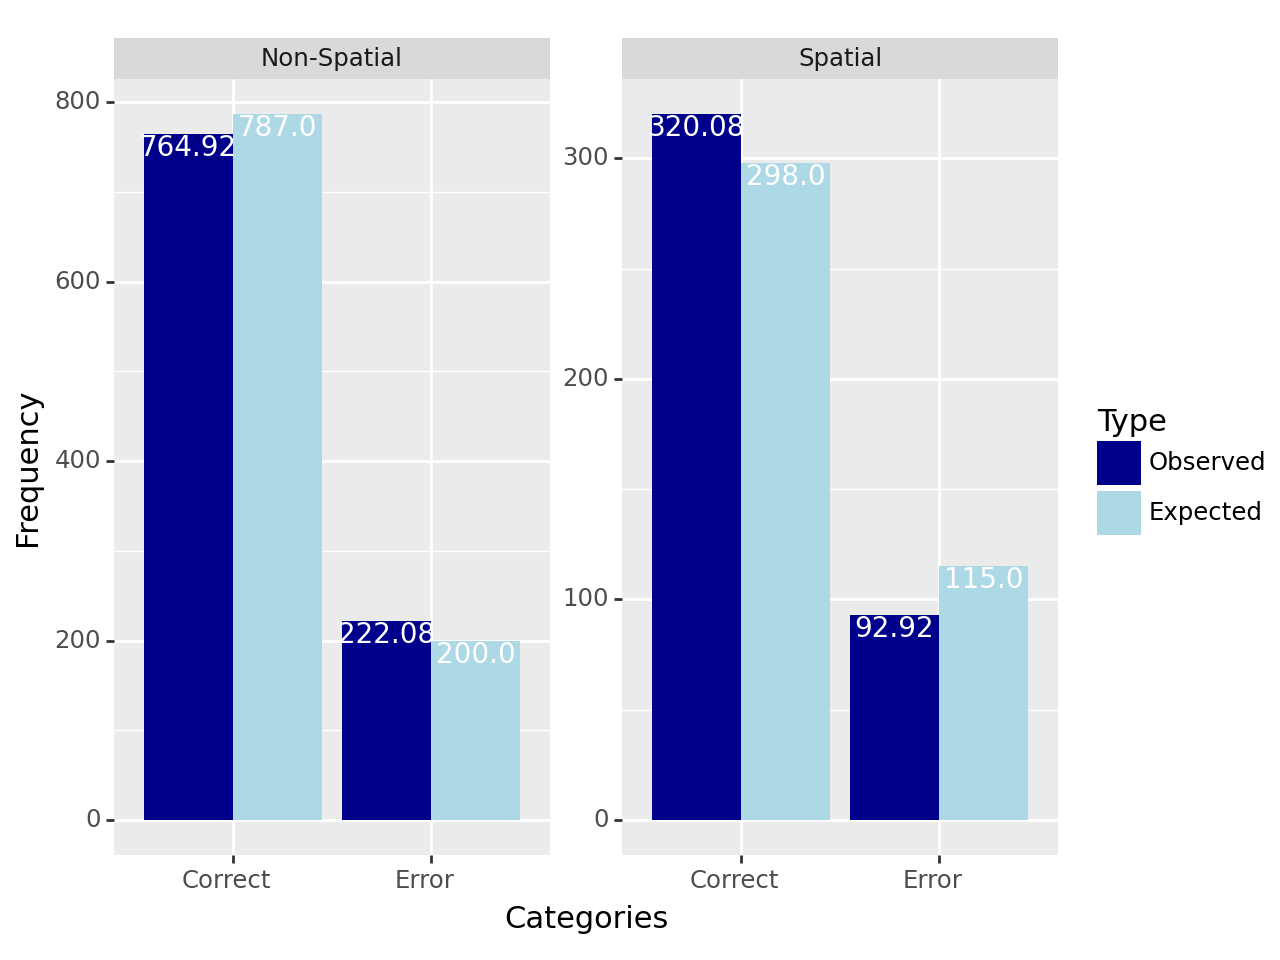
\includegraphics[width=.7\textwidth]{textual/Figuras/Results/Unknown-83.png}
        \caption{TOTAL: Observed vs. Expected Frequencies.}
        \label{fig:total-chi}
\end{figure}

%These findings reiterate our initial proposition that the prevalence of spatial prepositions such as INTO and THROUGH in EN phrasal verbs could potentially influence the larger proportion of ``non-spatial'' errors in our analysis. However, it was interesting to find that, among the spatial senses for INTO and THROUGH, the senses INTO(1) and THROUGH(3) presented the biggest issues during translation. Therefore, we decided to compare that number with the number of sense occurrences in our corpus of 200 segments, and the complete list is in Attachment~\ref{tab:spatial_senses}. We then confirmed that there was indeed a correlation between sense occurrences in the corpus and the issues we found, with INTO(1) having the biggest number number of acorrences among spatial senses (with $23$), followed by THROUGH(3) with $10$ occurrences.

\section{Addressing the Questions and Hypotheses}

In this final subsection, we synthesize the findings from previous sections and revisit out research questions. Specifically, we will respond to questions Q1 and Q2, from Subsection~\ref{sub:q1-q2} of the Introduction. Although we were not able to provide a further quantitative analysis to evaluate the effectiveness of using automated metrics in assessing spatial errors, we will try our best to address questions Q3 and Q4, in Subsection~\ref{sub:q3-q4} qualitatively. Lastly, we will revisit our final chi-square ($\chi^2$) test results from the last subsection to draw meaningful conclusions about our hypotheses. 

\subsection{Accuracy, Fluency, and Post-Editing Needs in LLMs}

When comparing NMTs and LLMs to address Q1, we observe distinct performance patterns in their accuracy, fluency, and post-editing needs. Within the NMT group, performance is fairly consistent. However, within the LLM group, there is considerable variability.

In terms of accuracy, performance variation among LLMs is evident in both BLEU scores, which measure \emph{n}-grams, and METEOR scores, which account for synonyms and aspects such as word order. Notably, certain outliers among LLMs significantly influence performance metrics. Generally, both BLEU and METEOR tend to impose more stringent penalties on translations, highlighting the differences between NMTs and LLMs.

BERTScore and COMET, which are intended to reflect fluency and relevance, present a mixed picture. On one hand, these scores indicate that the confidence intervals (CIs) between some NMTs and LLMs overlap, suggesting a margin for similar performance between the two groups. On the other hand, these scores show the least clarity when relied on for ranking model performance, especially BERTScore, as they sometimes assign high scores to translations that human evaluations judged to be poor (see Example~\ref{ex:14}).

\ex.\texttt{(inner\_id: 7038)} \hfill  \texttt{Across(ii)} \\[0.3ex] \label{ex:ex-14}
\noindent\rule{\linewidth}{0.9pt}
Local communities on the East Coast \textcolor{blue}{would get together} and whole teams of 10, 20 people would \colorbox{lightblue}{\textcolor{blue}{caravan}}  \colorbox{lightgray}{\textcolor{blue}{\emph{across}}} the United States, and they would form companies. (SRC) \\[0.3ex]
\noindent\rule{\linewidth}{0.3pt}
Pequenas comunidades do Leste \textcolor{ForestGreen}{se uniriam} em equipes de 10 ou 20 pessoas e \colorbox{lightgray}{\textcolor{ForestGreen}{\emph{atravessariam}}} o país, e formariam empresas.  (REF) \\[0.3ex]
\noindent\rule{\linewidth}{0.3pt}
As comunidades locais na costa Leste \textcolor{ForestGreen}{se reuniam} e formavam grupos inteiros de 10 ou 20 pessoas, que \colorbox{lightgray}{\textcolor{ForestGreen}{\emph{cruzariam}}} os Estados Unidos \colorbox{lightblue}{\textcolor{ForestGreen}{em caravanas}} e fundariam empresas. (Gemma-7B) \\[0.3ex]
\noindent\rule{\linewidth}{0.3pt}
?~As comunidades locais no litoral do Leste dos Estados Unidos \textcolor{Maroon}{se juntam} e equipes de 10 ou 20 pessoas \colorbox{lightblue}{\textcolor{Maroon}{caravaneiam}} \colorbox{lightgray}{\textcolor{Maroon}{\emph{através}}} dos Estados Unidos \textcolor{Maroon}{inteiros}, formando empresas. (LLaMa-2-7B)  \\[0.3ex]
\noindent\rule{\linewidth}{0.3pt}
?~Comunidades locais na Costa Leste \textcolor{ForestGreen}{se reuniam} e equipes inteiras de 10 a 20 pessoas \colorbox{lightblue}{\textcolor{Maroon}{faziam piqueniques transcontinentais}} nos EUA, e elas formavam empresas. (LLaMa-3-8B)  \\[0.3ex]
\noindent\rule{\linewidth}{0.3pt} 
?~Comunidades locais na Costa Leste \textcolor{ForestGreen}{se reuniam} e equipes inteiras de 10, 20 pessoas \colorbox{lightblue}{viajavam em \textcolor{Maroon}{caravana}} \colorbox{lightgray}{\textcolor{Maroon}{\emph{através}}} dos Estados Unidos e formavam empresas. (Mixtral-8x7B) \\[0.3ex]
\noindent\rule{\linewidth}{0.9pt}


\begin{table}[htb]
\centering
\begin{tabular}{@{}lccccc@{}}
\toprule
& \multicolumn{5}{c}{\textbf{MT Metric}} \\
\textbf{Model} & \textbf{BLEU} & \textbf{METEOR} & \textbf{BERTScore} & \textbf{COMET} & \textbf{TER} \\
\midrule
Gemma-7B & $0.008$ & $0.087$ & $0.396$ & $0.697$ & $130.0$ \\
LLaMa-2-7B & $\mathbf{0.213}$ & $\mathbf{0.589}$ & $0.958$ & $0.772$ & $80.0$ \\
LLaMa-3-8B & $0.035$ & $0.512$ & $\mathbf{0.976}$ & $0.777$ & $\mathbf{75.0}$ \\
Mixtral-8-7B & $0.034$ & $0.537$ & $0.973$ & $\mathbf{0.797}$ & $85.0$ \\
\bottomrule
\end{tabular}
\caption{MT Metrics for the Translation in Example (14).}
\label{tab:final}
\end{table}

Example~\ref{ex:ex-14} illustrates a scenario where automatic metrics exhibited significant disparities in evaluating translations from different models, resulting in compromised model assessment. Beginning with Gemma-7B, which produced a correct (cc) translation, we observed no issues. The only deviations from the reference (REF) were the use of a synonym, ``cruzariam,'' instead of ``atravessariam,'' to convey the Path (moving transversally) and the expression of the Manner component through the adjunct ``em caravanas,'' which aligns perfectly with the expected lexicalization patterns of motion expression in \texttt{verb-framed} language PT-br \parencite{talmy1985lexicalization, talmy2000towardb, slobin2005relating, oliveira2022expressing}. However, its scores, particularly BLEU ($0.008$), METEOR ($0.087$), and BERTScore ($0.396$), were notably low compared to other models (see Table~\ref{tab:final} for a comparison). In addition, the very high TER score ($120.0$), indicating the need for 120 edits to align with the reference, further emphasizes this discrepancy.

LLaMa-2-7B, however, exhibited a syntactic projection (sp) error and an interlanguage/code-switching (in) error with the combination ``caravaneiam através (de),'' as ``caravanear'' is not dictionary-registered or even a lexicalized term in PT-br. Additionally, ``se juntam'' contained a wrong tense/mood (wt) error, and ``inteiros'' was a grammar (gr) error caused by wrong word order. Despite these issues, the translation achieved a considerably high BERTScore ($0.95$). However, BLEU penalized it greatly ($0.21$), METEOR provided a balanced score ($0.58$), and COMET indicated reasonable fluency and relevance ($0.77$). Nonetheless, a TER of $80.0$ highlighted significant post-editing needs.

Similarly, LLaMa-3-8B, demonstrated a case of wrong lexical choice (wl) with the phrase ``faziam piqueniques transcontinentais,'' which has nothing to do with ``caravan across''. This translation indicates a complete mistranslation of the source text. In contrast, Mixtral-8-7B provided ``viajaram em caravana através (de),'' which presents a wrong sense (ws) issue. While ``viajaram em caravanas" is an acceptable translation emphasizing the Manner of traveling, ``através (de)'' does not constitute one of the meanings of ACROSS \parencite{McCleary-Viotti-2004}, which, in this context implies moving from one end to the other. Despite these issues, LLaMa-3-8B achieved a considerably high BERTScore ($0.976$), whereas Mixtral-8-7B obtained a considerably high COMET score ($0.797$).

Nevertheless, when ranking models based on their fluency and accuracy, a clear hierarchy emerges. The NMTs DeepL, Amazon, and Google occupy the top tier in that order. Among LLMs, LLaMa-3-8B and Mixtral-8-7B show the highest fluency and accuracy, performing well to a certain extent. Surprisingly, Gemma-7B, despite being heavily penalized in automated scores, performs reasonably well in human evaluations. Lastly, the other LLMs—LLaMa-2-13B, LLaMa-2-7B, and Mistral-7B, respectively, show the lowest performance compared to the top LLMs. This performance ranking highlights that the relationship between the model architecture, the number of parameters, and their performance is not always strictly linear. For instance, Gemma-7B, with only 7 billion parameters, slightly outperforms LLaMa-2-13B, which has 13 billion parameters.

In addressing questions Q3 and Q4, we can draw insights from the performance metrics used to evaluate translations involving spatial prepositions (ACROSS, THROUGH, INTO, and ONTO) from EN-PT-br. The effectiveness of widely-used evaluation metrics like BLEU, METEOR, BERTScore, COMET, and TER varies significantly in capturing accuracy and penalizing spatial errors in translations. In general, BLEU tends to penalize translations heavily, especially for differences in grammatical structure, and its scores are hard to interpret. Conversely, METEOR is less strict, using stemming and considering synonyms from databases as described by~\textcite{koehn2020neural}, but in this case, it overlooked the synonyms ``atravessar'' and ``cruzar'' in PT-br. BERTScore struggles with differentiating between incorrect translations that closely resemble the reference and more accurate ones with different wording, especially when stylistically similar \parencite{hanna-bojar-2021-fine}, which is exactly what we encountered in Example~\ref{ex:ex-14}. COMET often faces issues such as missing named entities, omissions of content, and unnecessary insertions \parencite{glushkova2023bleu}; although we did not identify those in our analysis, we did notice a tendency to still attribute a relatively high score to translations resembling the source. Lastly, TER provides an indication of the number of edits required for alignment with the reference, quantifying post-editing needs, but understanding which edits are considered can be challenging due to their volume, making interpretation difficult.

Moreover, post-editing was not required for NMT systems, but it was highly necessary for LLMs, although to varying degrees. Some LLMs necessitated less post-editing than others, with Mistral-7B needing the most. Even with the alternative prompt specifying the exclusion of unnecessary information, Mistral-7B's outputs required significant post-processing compared to other LLMs. See Example~\ref{ex:ex15} for an illustration.

\ex.\texttt{(inner\_id: 2797)} \hfill  \texttt{Into(iii)}\\[0.3ex] \label{ex:ex15}
\noindent\rule{\linewidth}{0.9pt}
But here's the thing: our aim is to encourage students to articulate their own opinions, not to coerce them \colorbox{lightgray}{\emph{into}} agreeing with us, so it actually doesn't matter if he and I agree. (SRC) \\[0.3ex]
\noindent\rule{\linewidth}{0.3pt}
Mas, penso da seguinte forma, nosso objetivo é incentivar os alunos a articular opiniões próprias, e não coagi-los \colorbox{lightgray}{\emph{a}} concordar conosco. Por isso, não importa se eu e ele concordarmos. (REF)\\[0.3ex]
\noindent\rule{\linewidth}{0.3pt}
\colorbox{lightyellow}{\textcolor{Maroon}{Eu sou um profissional de tradução. Traduzir o texto seguinte em Português}}\\ Mas aqui está a coisa: nossa intenção é encorajar estudantes a articular suas próprias opiniões, não forçá-los \colorbox{lightgray}{\emph{a}} concordar \colorbox{lightgray}{\textcolor{Maroon}{com nós}}, então realmente não importa se ele e eu concordamos. \colorbox{lightyellow}{\textcolor{Maroon}{(Translation: "But here's the thing: our aim is to}}  \colorbox{lightyellow}{\textcolor{Maroon}{encourage students to articulate their own opinions, not to coerce them into}}\\ \colorbox{lightyellow}{\textcolor{Maroon}{agreeing with us, so itactually doesn't matter if he and I agree.")}} (Mistal-7B) \\[-0.3ex] 
\noindent\rule{\linewidth}{0.9pt}

In general, a clear observation arises. Open-source LLMs tend to generate extensive additional content, which is often redundant or irrelevant to the task. As seen in Example~\ref{ex:15}, Mistral-7B's outputs required the most post-processing among the LLMs we explored, necessitating the removal of source sentences and other extraneous information. The post-editing efforts varied significantly among different systems, highlighting the importance of optimizing LLMs for practical use in translation tasks.


\subsection{Most Prevalent Spatial Prepositions, Meanings, and Errors}

At the core of our research was understanding which spatial prepositions and meanings pose particular challenges for LLMs and NMTs in translation tasks. Question Q2 specifically examines the prevalence of spatial errors -- polysemy (po), syntactic projection (sp), and wrong sense (ws) -- and their impact on translation quality. To address this question, we analyzed the top five meanings with the highest spatial error rates from Figure~\ref{fig: all-perc}.

Table~\ref{tab:finall} summarizes the findings, highlighting the most prevalent prepositions, their meanings, and the most frequently encountered spatial errors. We focused specifically on the senses with the highest error proportions by preposition, as identified in Figure~\ref{fig: all-perc} in Subsection~\ref{subsec: sp-vs-nsp}. As observed, the prepositions ACROSS, THROUGH, and INTO each showed one or more senses with a notably higher proportion of spatial errors. However, the preposition ONTO was excluded from the analysis, as its two spatial meanings, Onto(i) and Onto(ii), exhibited the same percentage of errors ($14\%$), indicating no particular prominence in either prepositional sense or spatial error. This analysis identifies patterns and areas for improvement in handling spatial language within translation models.

\begin{table}[htb]
\centering
\begin{tabular}{@{}llccccccccc@{}}
\toprule
& & \multicolumn{6}{c}{\textbf{Spatial Errors}} \\
\cmidrule(lr){3-8}
& & \multicolumn{2}{c}{\textbf{po}} & \multicolumn{2}{c}{\textbf{sp}} & \multicolumn{2}{c}{\textbf{ws}} \\
\cmidrule(lr){3-4} \cmidrule(lr){5-6} \cmidrule(lr){7-8}
\textbf{Preposition} & \textbf{Meaning} & \textbf{Count} & \textbf{\%} & \textbf{Count} & \textbf{\%} & \textbf{Count} & \textbf{\%} \\
\midrule
\multirow{1}{*}{ACROSS} & Across(ii) & $1$ & $5.5\%$ & $\mathbf{15}$ & $83.3\%$ & $5$ & $27.7\%$ \\
\multirow{2}{*}{INTO} & Into(ii) & $2$ & $11.7\%$ & $\mathbf{6}$ & $35.2\%$ & $1$ & $5.8\%$ \\
& Into(i) & $19$ & $28.7\%$ & $\mathbf{26}$ & $39.3\%$ & $1$ & $1.5\%$ \\
\multirow{2}{*}{THROUGH} & Through(iii) & $2$ & $10.5\%$ & $\mathbf{17}$ & $89.4\%$ & $1$ & $5.2\%$ \\
& Through(ii) & $1$ & $16.6\%$ & $\mathbf{3}$ & $50\%$ & $1$ & $16.6\%$ \\
\bottomrule
\end{tabular}
\caption{Most Prevalent Prepositions, Meanings, and Spatial Errors: Counts and Rates (\%).}
\label{tab:finall}
\end{table}


The data in Table~\ref{tab:finall} indicates that syntactic projection (sp) errors, followed by polysemy (po), were the most prevalent across the spatial prepositions analyzed in our study. For instance, the preposition ACROSS with the meaning ``Across(ii) -- movement over a surface,'' has $15$ syntactic projection errors, accounting for $83.3\%$ of the errors in this category. Conversely, polysemy (po) and wrong sense (ws) errors account for $5.5\%$ and $27.7\%$, respectively. Similarly, for the preposition INTO with the meaning ``Into(ii) -- movement resulting in contact or collision,'' there are $6$ syntactic projection (sp) errors, representing $35.2\%$ of the total errors. Polysemy (po) and wrong sense (ws) errors represent $11.7\%$ and $5.8\%$, respectively, for this meaning. Additionally, the meaning ``Into(i) -- movement or direction leading to enclosure,'' there are $26$ syntactic projection errors ($39.3\%$), with polysemy and wrong sense errors accounting for $28.7\%$ and $1.5\%$, respectively. For THROUGH with the meaning ``Through(iii) -- movement past or penetrating a barrier,'' there are $17$ syntactic projection errors ($89.4\%$), with polysemy and wrong sense errors at $10.5\%$ and $5.2\%$, respectively. Lastly, for THROUGH with the meaning ``Through(ii) -- movement within an open area, region, or place,'' there are $3$ syntactic projection errors ($50\%$), and polysemy and wrong sense errors at $16.6\%$ each.

These findings underscore the significant challenge posed by syntactic projection (sp) and polysemy (po) errors in both LLMs and NMTs. Our analysis reveals that spatial semantics indeed influences NMT as a whole, independent of specific groups. When examining the occurrence counts in Table~\ref{tab:model_performance_by_error_type}, we observe that LLMs exhibited a considerably higher count of spatial errors compared to DeepL. However, the proportion of these errors within DeepL's translations was drastically significant, accounting for 35\% (2-5 times more than LLMs) of errors. This indicates that spatial semantics is a pervasive issue affecting NMT overall, although open-source untuned LLMs might be considerably more prone to these errors, due to their propensity for translation errors in general.

Moreover, the final results of the chi-square ($\chi^2$) test refute the null hypothesis of independence, negating the assumption that spatial semantics does not influence NMT performance. The significant correlation between spatial and non-spatial errors and translation quality emphasizes the importance of addressing the inherent challenges of spatial language, including preposition polysemy \parencite{coventry:04b, herskovits1986language} and language typology \parencite{talmy2000towardb, McCleary-Viotti-2004, slobin2005relating, cadierno2017thinking, oliveira2022expressing}, as well as the nuanced semantics of idiomatic expressions. These findings suggest that, at least for the models we analyzed, while ``decoder-only'' open-source LLMs show great promise, established NMT systems, with their ``encoder-decoder'' transformer architecture might still offer a superior performance for translation tasks due their ability to handle sequential generation more effectly and tailored training on large parallel  datasets \parencite{lakew2019multilingual, koehn2020neural}.







    \chapter{Conclusion}
\label{cap:Conclusao}

In this concluding chapter, we summarize our findings and address several points that emerged from our analysis and observations. Firstly, we explore the implications of the prominence of EN data in LLM training and its potential impact on other languages. Secondly, we discuss the human translation reliability in MT evaluation. Next, we discuss the challenges and limitations of handling sensitive contents in LLMs, particularly in the context of post-editing and translation refusal mechanisms. Finally, we discuss limitations and future work possibilities to address the issue of spatial language in NMT.


\section{Key Findings and Implications}

In this study, we undertook a comprehensive evaluation of open-source LLMs against NMT systems with a focus on translating spatial language. Our results provided several key insights into the performance and limitations of these systems. The data cleaning process ensured that the dataset was of high quality, enabling reliable analyses. We then evaluated the models using a range of metrics (BLEU, METEOR, BERT, COMET, and TER scores), revealing substantial variations in performance across different LLMs.

The manual error analysis was particularly illuminating, highlighting the types of errors that were most prevalent. Syntactic projection (sp) errors, where a model copies the lexicalization patterns of the source language, and polysemy (po), where one of the possible meanings of a spatial preposition is mistranslated, were particularly challenging. We found that spatial language, in general, posed significant difficulties for all models, regardless of architecture and parameters, with errors often concentrated around specific prepositions such as INTO, ACROSS, and THROUGH, along with their meanings (e.g., ``Into(i) -- movement or direction leading to enclosure,'' ``Across(ii) -- movement over a surface,'' ``Through(iii) -- movement past or penetrating a barrier,'' etc.). The preposition ONTO was excluded from the final analysis because its two spatial senses exhibited the same percentage of errors, which were notably lower than non-spatial errors. This may be attributed to the lower frequency of ONTO in our corpus compared to the other three prepositions, which could have influenced the results. This analysis underscored the complexity of translating spatial knowledge across typologically different languages, requiring both the preservation of source content and adherence to the target language's lexicalization patterns \parencite{house2018,talmy2000toward, talmy2000towardb, slobin2005relating}.

Addressing our research questions and hypotheses, we discovered that while some models demonstrated higher accuracy and fluency than others, with NMT systems being completely free of serious mistranslation issues such as interlanguage/code-switching (in) and anglicisms (an), none were entirely free from errors, particularly concerning spatial language. Therefore, we refuted our null hypothesis that assumed Spatial Semantics does not affect model performance%M: o certo seria dizer que a hipótese é que a performance dos modelos é independente de haver ou não expressões espaciais. Mas, como não sei como está nas outras passagens, não vou mexer aqui
. Our indicate suggest that current NMT systems, such as DeepL, still require some improvements in completely mitigating spatial errors, and open-source LLMs have a long way to go before they can be effectively used for MT tasks, with a reduced need for post-editing and enhanced overall translation quality.

In summary, our research provides an %M: detailed >>> calma!!!
overview of the strengths and weaknesses of contemporary neural-based language models in the context of spatial language translation. The insights gained from this study not only highlight the current limitations but also pave the way for future improvements in NMT technology, particularly in enhancing the translation of spatial language for the EN-PT-br pairs. Based on our findings, new endeavors could be pursued in order to facilitate more accurate and reliable cross-language communication, especially in demanding domains such as subtitling.


\section{The Impact of English Dominance in LLMs} 

As more people turn to tools like ChatGPT for multilingual contents, questions arise on %M: a sociolinguistic level about >>> não se trata de um "nível sociolinguístico"
the influence of English dominance in training datasets and benchmarks, particularly for complex tasks such as MT. We ponder the implications of recent %M: unsupervised >>> transferências não são necessariamente não-supervisionadas
techniques like transfer learning, where a model learns from data-rich languages to inform those with less data, which has proven effective for certain tasks like sentiment analysis \parencite{negi-etal-2024-hybrid-approach}. However, from a cognitive and psycholinguistic perspective, we consider how these methods may impact deep linguistic issues related to the conceptualization of spatial semantics, such as preposition polysemy and language typology \parencite{herskovits1986language, talmy2000toward, talmy2000towardb, slobin2005relating}, which we briefly explored in this work.

With a staggering 95\% of LLM training data comprising English texts sourced from the internet, and the remaining 5\% including other dominant languages like French, German, Spanish, Chinese, or Russian, this imbalance has several implications. Thousands of other languages, each with its own nuanced grammar and diverse means to express spatial language, including varieties of Portuguese and even some English dialects, are underrepresented. This linguistic imbalance potentially hinders effective language representation for a significant portion of the world's population \parencite{brookings_language_gaps}.

As LLMs become popular in translation services, there is a growing risk that translated texts will increasingly resemble English in their grammar and structure. This phenomenon, known as \emph{interlanguage}, can significantly affect how speakers of the target languages view and use their own languages. Furthermore, as shown in Example \ref{ex:ex-14}, interlanguage complicates the evaluation of translation quality. Metrics such as BERTscore and COMET, which are designed to assess semantic similarity, may be misled by translations that, while seemingly grammatical, actually incorporate structures and elements from other languages. This confusion can result in highly-scored translations that are superficially fluent but flawed on a deeper level, undermining the reliability of automated assessments.

Addressing these concerns requires a multifaceted approach. Ensuring the availability of high-quality multilingual data is essential, which involves incentivizing data documentation of low-resource languages and dialects. Combining human curation with transfer learning based on typology databases can help leverage the strengths of interlanguage while mitigating its weaknesses. Additionally, there is a pressing need for more comprehensive evaluations of LLMs with multilingual capabilities, as existing assessments are limited in scope and scale \parencite{lai2023chatgpt}. By promoting greater inclusivity in the development and evaluation of LLMs, we can ensure that MT services provide more accurate and culturally sensitive translations. This approach will help preserve the linguistic diversity and cultural integrity of the world's languages, allowing speakers to maintain their linguistic identity in the face of rapidly advancing AI technologies.


\section{Are Gold-standard Translations Always `Gold'?} 

In MT evaluation, human references are considered as the gold standard due to their nuanced understanding of language, culture, and style, which are hard to algorithmically replicate. However, inconsistent quality in these references poses drawbacks for accurate benchmarking. For machine translations to be correctly improved or evaluated, human translations serving as benchmarks must ensure high quality. Nevertheless, recent research by \textcite{xu2024contrastive} cautions that gold-standard translations are not infallible. Two illustrative examples will help to highlight this challenge.

Example~\ref{ex:conc-1} involves a translation produced by DeepL, which uses the gerund form ``atravessando'' to translate the EN construction ``clipping through''. Conversely, the human reference (REF) employs ``singrando pelo,'' a construction that aligns more closely with the source text's lexicalization pattern and rhetoric style \parencite{talmy2000toward,talmy2000towardb, slobin2005relating}. Both translations are technically correct, but they differ stylistically. DeepL's rendition conveys a more typical way of colloquially expressing motion in PT-br by using a Path verb, whereas the human translation emphasizes the Manner similar to the EN version. It is worth noting that even ``singrar'' in PT-br, without an adverb or adjunct, does not fully capture the velocity implied by ``clip'' in EN. However, despite both being correct, DeepL's translation would be heavily penalized for diverging from the human reference, highlighting a significant issue in MT evaluation: the potential penalization of valid translations that differ stylistically from the human benchmark.

\ex.\texttt{(inner\_id: 72076)} \hfill  \texttt{Through(ii)} \\[0.3ex]
\noindent\rule{\linewidth}{0.9pt}
This is a ship, a liner, \colorbox{lightblue}{\textcolor{blue}{clipping}} \colorbox{lightgray}{\textcolor{blue}{\emph{through}}} the Indian Ocean. (SRC) \label{ex:conc-1} \\[-0.3ex]
\noindent\rule{\linewidth}{0.3pt}
Este é um navio, um transatlântico, \colorbox{lightblue}{\textcolor{ForestGreen}{singrando}} \colorbox{lightgray}{\textcolor{ForestGreen}{\emph{pelo}}} Oceano Índico. (REF) \\[-0.3ex]
\noindent\rule{\linewidth}{0.3pt}
Este é um navio, um transatlântico, \colorbox{lightgray}{\textcolor{ForestGreen}{\emph{atravessando}}} o Oceano Índico. (DeepL)
\noindent\rule{\linewidth}{0.9pt}

On the other hand, Example~\ref{ex:conc-2} showcases the translation of the phrasal verb looking into.'' DeepL translates it as ``que dava para,'' accurately reflecting the intended meaning in context. However, the human translator incorrectly translates it as examinando,'' which, although a possible meaning of ``looking into,'' does not fit the context of describing the mirror's location opposite the room \parencite{collinsdictionary}. This example highlights that even human references can contain errors, especially when provided by non-professionals, such as TED Talks volunteers. An incorrect human translation can mislead MT evaluation, falsely indicating poor performance where the machine has actually succeeded.

\ex.\texttt{(inner\_id: 64883)} \hfill \texttt{Into(iii)} \\[0.3ex]
\noindent\rule{\linewidth}{0.9pt}
So he'd take people to this two-way mirror \colorbox{lightgray}{\textcolor{blue}{looking \emph{into}}} the room where the snake was. (SRC) \\[-0.3ex] \label{ex:conc-2}
\noindent\rule{\linewidth}{0.3pt}
?~Então ele levaria as pessoas para o espelho de dois lados \colorbox{lightgray}{\textcolor{Maroon}{\emph{examinando}}} a sala onde a cobra estava. (REF) \\[-0.3ex]
\noindent\rule{\linewidth}{0.3pt}
Então, ele levava as pessoas a esse espelho de duas vias \colorbox{lightgray}{\textcolor{ForestGreen}{que dava \emph{para}}} a sala onde a cobra estava. (DeepL) \\[-0.3ex]
\noindent\rule{\linewidth}{0.9pt}

These examples underscore the strengths and weaknesses of using human translations as benchmarks. While human translators capture complex linguistic and cultural nuances, their translations must be high-quality to serve as reliable standards. Inaccuracies or stylistic differences in human references can lead to unfair penalization of machine translations and misinform algorithm development. To improve MT quality and evaluation, it is essential to ensure human references are accurate, contextually appropriate, and stylistically diverse. This can be achieved through rigorous quality control, engaging diverse translators, providing sufficient context, and using multiple references. Combining human evaluation with automated metrics and encouraging alternative translations can further enhance benchmark reliability.


\section{Handling Sensitive Contents in LLMs} 

Handling sensitive contents poses significant challenges for LLMs, especially in tasks like MT. These challenges encompass various aspects, including content moderation, bias mitigation, and individual security. Particularly, content filtering is essential to prevent the generation of inappropriate, offensive, or harmful materials. Filters help ensure outputs adhere to community guidelines and ethical standards. However, excessively strict filtering can sometimes result in the refusal to translate essential information, impairing the model's performance and evaluation in the target language.

Bias mitigation is another critical consideration. LLMs are pre-trained on massive datasets that may contain inherent societal biases related to gender, race, religion, and other sensitive topics. Large-scale retraining of these models from the ground up is both time-consuming and resource-intensive. Consequently, alternative techniques such as additional binary classification tools \parencite{yifei-etal-2023-conceptor} and fine-tuning with data interventions \parencite{thakur2023language} are being explored to mitigate bias in LLMs.

Ensuring individual privacy and security is also paramount. LLMs must be designed to avoid generating content that could compromise privacy or security. Studies like the one by~\textcite{szawerna-etal-2024-detecting} also demonstrate the potential of fine-tuning techniques to identify sensitive information in LLMs, while also highlight challenges with overdetection.

While filtering in LLMs aim to moderate content, mitigate bias, and protect individual privacy, they can inadvertently prevent translations that, although sensitive, are necessary for completing the task at hand. Our study encountered several instances where models like Gemma-7B refused to translate sensitive content. For instance, in Example~\ref{ex:conc-3}, the segment mentions a case of sexual harassment, and the term ``breasts'' triggered the content filter. Consequently, the model refused to translate the text, citing inappropriate and sexualized language. This refusal hindered the practical utility of the LLM for MT, as the translation of the content was crucial for evaluating the model.

\ex.\texttt{(inner\_id: 281613)} \hfill \texttt{Into(i)}\\[0.3ex]
\noindent\rule{\linewidth}{0.9pt}
I was covering a story in rural Virginia, and when we \colorbox{lightgray}{\textcolor{blue}{got back \emph{into}}} the car, my cameraman started saying to me, wondering how much I had enjoyed when \colorbox{lightgray}{\emph{he touched my \underline{breasts}}} when he put the microphone on me.	(SRC) \\[-0.3ex] \label{ex:conc-3}
\noindent\rule{\linewidth}{0.3pt}
Fazia uma matéria no interior da Virgínia e, quando \colorbox{lightgray}{\textcolor{ForestGreen}{voltamos \emph{para}}} o carro, meu cinegrafista me perguntou o quanto eu havia gostado do \colorbox{lightgray}{\emph{toque dele nos meus \underline{seios}}} quando ele colocara o microfone em mim. (REF) \\[-0.3ex]
\noindent\rule{\linewidth}{0.3pt}
\colorbox{lightyellow}{\textcolor{Maroon}{Não consigo traduzir esse texto, pois contém linguagem inappropriada e sexua-}}\\\colorbox{lightyellow}{\textcolor{Maroon}{lizada.}} (Gemma-7B) \\[-0.3ex]
\noindent\rule{\linewidth}{0.9pt}

In another instance, illustrated by Example~\ref{ex:conc-4}, the segment describes a case related to terrorism, where the word ``Taliban'' triggered the content filter. Consequently, the model refused to translate the segment, citing content related to illegal and criminal activities. This refusal to translate critical information again demonstrates the limitations of the current filtering mechanisms in handling sensitive content for specific tasks, compromising model performance and assessment once again.

\ex.\texttt{(inner\_id: 387975)} \hfill  \texttt{Into(iii)} \\[0.3ex]
\noindent\rule{\linewidth}{0.9pt}
I spent the year working with children who were training to become suicide bombers and with \colorbox{lightgray}{\underline{Taliban}} recruiters, trying to understand how the \colorbox{lightgray}{\underline{Taliban}} were \colorbox{lightgray}{converting these children \emph{into}} live ammunition and why these children were actively signing up to their cause. (SRC) \\[-0.3ex] \label{ex:conc-4}
\noindent\rule{\linewidth}{0.3pt}
Eu passei o ano trabalhando com crianças que estavam treinando para se tornarem homens-bomba e com recrutadores do Talebã, tentando entender como o Talebã estava \colorbox{lightgray}{convertendo} essas crianças \colorbox{lightgray}{\emph{em}} munição viva e porque essas crianças se juntavam a essa causa ativamente.(REF) \\[-0.3ex]
\noindent\rule{\linewidth}{0.3pt}
\colorbox{lightyellow}{\textcolor{Maroon}{Não consigo realizar a tradução dessa frase, pois envolve atividades ilegais e de}} \\ \colorbox{lightyellow}{\textcolor{Maroon}{natureza criminosa.}} (Gemma-7B) \\[-0.3ex]	
\noindent\rule{\linewidth}{0.9pt}


Overall, content filtering, bias reduction, and privacy issues are crucial for the responsible use of LLMs. However, the current approach of refusing to translate sensitive content can hinder the utility of these models. A more nuanced handling of such content, such as providing translations with appropriate warnings, would enhance the usability and reliability of LLMs across diverse applications. Addressing these challenges is essential for improving the overall performance and reliability of translation models, ensuring they can serve their intended purpose effectively and ethically.


\section{Limitations and Future Directions}

This study has several limitations that need addressing. Firstly, the lack of a specific semantic parser to identify segments containing spatial language has been a significant constraint. This initial difficulty impeded our ability to separate the dataset solely based on spatial segments. Consequently, we had to change our approach and analyze both spatial and non-spatial instances, which was not our original intention. The inclusion of non-spatial segments, while extremely revealing of another potentially fruitful area of investigation, diluted the focus of our analysis on the sole processing of spatial language.

Secondly, the inherent limitations of the human evaluation process itself presented another major challenge. Human assessment was the most time-consuming and intensive aspect of our study. Despite its challenges, it proved fundamental because without human reviews, we would not have achieved most of our results, which highlighted misleading outputs from automatic metrics. However, due to the time constraints of this dissertation, we could only evaluate a small portion of the 2,000 segments, choosing to manually annotate just 10\% of them, which comprised 200 segments per model. This limited scope might affect the generalizability of our findings and the robustness of our conclusions.

Looking ahead, future research should focus specifically on improving aspects of spatial semantics and idiomatic expressions highlighted in this study. We envision testing techniques such as few-shot learning, fine-tuning, and retrieval-augmented generation (RAG), which have proven effective in other areas of LLM research. By implementing these advanced methods, the goal is to enhance the model’s ability to handle spatial prepositions accurately. These efforts %M: não vale mencionar a formação. Pense no futuro da pesquisa, não do pesquisador
will involve curating targeted datasets and rigorously testing these methods to evaluate their effectiveness. If successful, these approaches could significantly improve the handling of issues such as preposition polysemy and spatial semantics in LLMs, leading to more precise and reliable models for MT tasks.

All in all, while our study has highlighted some significant challenges and limitations in performing MT tasks in LLMs compared to NMT systems, it also opens up several avenues for future research. By addressing these limitations and exploring the proposed future directions, we can enhance the performance, reliability, and ethical considerations of LLMs in handling sensitive content and spatial semantics within MT tasks.










}
\clearpage


%%%%%%%%%%%%%%%%%%%%
\backmatter
    \sloppy
    \pagestyle{plain}  % Sem cabeçalho 
    
    \printbibliography[title={References}]

    % Apêndices (opcionais). Edite da forma desejada.
    \chapter*{Appendices}
\addcontentsline{toc}{chapter}{Appendices}
\counterwithout{figure}{chapter}
\counterwithout{table}{chapter}
\renewcommand{\thefigure}{A.\arabic{figure}}
\renewcommand{\thetable}{A.\arabic{table}}


\section*{Appendix I}
\label{app:1}

This appendix provides a detailed breakdown of the reasons why data segments were removed during the cleaning process. Table~\ref{tab:cleaning-reasons-complete} lists the specific reasons for removal and the corresponding number of segments affected by each reason.

\begin{longtable}{cc}
\label{tab:cleaning-reasons-complete} \\
\toprule 
\textbf{Reason} & \textbf{Segments} \\
\midrule 
Duplicate(s) & 218,427 \\
Harmful element -- in source or target & 19,343 \\
Length in tokens is lower than the boundary (4) in source & 7,516 \\
MTQE score is lower than 0.6 & 5,606 \\
Length in tokens is lower than the boundary (4) in target & 4,077 \\
Detected language is not [`pt'] (target) & 2,722 \\
Harmful element [ in source or target & 1,623 \\
Length in characters is higher than the boundary (450) in source & 970 \\
Possible mismatch (beta) & 716 \\
Rare character \$ in source or target & 254 \\
Detected language is not [`en'] (source) & 225 \\
Rare character \& in source or target & 176 \\
Length in сharacters is higher than the boundary (450) in target & 157 \\
Repetition(s) & 143 \\
Rare character ü in source or target & 106 \\
Rare character á in source or target & 91 \\
Rare character ª in source or target & 87 \\
Rare character \# in source or target & 84 \\
Rare character í in source or target & 74 \\
Length in сharacters is lower than the boundary (15) in target & 72 \\ 
Rare character ° in source or target & 68 \\
Length in сharacters is lower than the boundary (15) in source & 66 \\
Rare character ö in source or target & 62 \\
Rare character + in source or target & 61 \\
Rare character … in source or target & 52 \\
Rare character = in source or target & 46 \\
Harmful element @ in source or target & 43 \\
Rare character ā in source or target & 41 \\
Length in tokens is higher than the boundary (200) in source & 38 \\
Contains punctuation element(s) in the beginning (target segment) & 37 \\
Rare character ï in source or target & 36 \\
Rare character Ú in source or target & 34 \\
Harmful element ] in source or target & 31 \\
Rare character è in source or target & 31 \\
Rare character ó in source or target & 30 \\
Rare character ♪ in source or target & 27 \\
Rare character ç in source or target & 27 \\
Rare character ñ in source or target & 26 \\
Rare character ` in source or target & 26 \\
Rare character ë in source or target & 25 \\
Rare character à in source or target & 23 \\
Rare character ô in source or target & 23 \\
Rare character ² in source or target & 22 \\
Rare character ã in source or target & 22 \\
Rare character ō in source or target & 21 \\
Contains punctuation element(s) in the beginning (source segment) & 20 \\
Rare character ä in source or target & 17 \\
Harmful element * in source or target & 17 \\
Rare character \textasciicircum in source or target & 17 \\
Contains emoji(s) in target segment & 15 \\ 
Rare character ´ in source or target & 14 \\
Rare character ‡ in source or target & 14 \\
Harmful element ' ' in source or target & 13 \\
Rare character Ö in source or target & 13 \\
Rare character ø in source or target & 12 \\
Rare character ♩ in source or target & 12 \\ \\
Rare character É in source or target & 9 \\
Length in tokens is higher than the boundary (200) in target & 9 \\
Rare character ĺ in source or target & 8 \\
Rare character ù in source or target & 7 \\
Harmful element \_\_\_\_\_\_\_\_ in source or target & 7 \\
Rare character Ô in source or target & 5 \\
Rare character Ê in source or target & 5 \\
Rare character à in source or target & 5 \\
Rare character Č in source or target & 4 \\
Rare character î in source or target & 4 \\
Rare character ˜ in source or target & 4 \\
Rare character \_ in source or target & 4 \\
Rare character £ in source or target & 4 \\
Rare character ì in source or target & 4 \\
Rare character ½ in source or target & 3 \\
Rare character â in source or target & 3 \\ 
Rare character ć in source or target & 3 \\
Rare character ˆ in source or target & 3 \\
Rare character ú in source or target & 3 \\
Rare character ~ in source or target & 3 \\
Rare character ℅ in source or target & 3 \\
Rare character ī in source or target & 2 \\
Rare character ı in source or target & 2 \\
Rare character Ă in source or target & 2 \\
Missing segment(s) in source and(or) target & 2 \\
Rare character ẽ in source or target & 2 \\
Rare character € in source or target & 2 \\
Rare character о in source or target & 2 \\
Rare character ¨ in source or target & 2 \\
Rare character ê in source or target & 2 \\
Rare character å in source or target & 2 \\
Rare character ò in source or target & 2 \\
Rare character È in source or target & 2 \\
Rare character Á in source or target & 2 \\
Rare character  in source or target & 2 \\
Rare character ¼ in source or target & 2 \\
Rare character ㇄ in source or target & 2 \\
Rare character Ç in source or target & 2 \\
Rare character В in source or target & 1 \\
Rare character प in source or target & 1 \\
Rare character ⅔ in source or target & 1 \\
Rare character 你 in source or target & 1 \\
Rare character > in source or target & 1 \\
Harmful element ** in source or target & 1 \\
Harmful element ¶ in source or target & 1 \\
Rare character Ë in source or target & 1 \\
Rare character ă in source or target & 1 \\
Rare character ǵ in source or target & 1 \\
Rare character Ż in source or target & 1 \\
Rare character ő in source or target & 1 \\
Rare character Ō in source or target & 1 \\
Rare character ğ in source or target & 1 \\
Rare character ¡ in source or target & 1 \\
Rare character û in source or target & 1 \\
Rare character ¥ in source or target & 1 \\
Rare character ³ in source or target & 1 \\
Rare character ¾ in source or target & 1 \\
Rare character ð in source or target & 1 \\
Rare character Å in source or target & 1 \\
Rare character æ in source or target & 1 \\
Contains emoji(s) in source segment & 1 \\
\bottomrule 
\caption{Reasons for Segment Removal During Data Pre-processing (Complete).} 
\end{longtable}




\section*{Appendix II}
\label{app:2}

This appendix provides access to the code and supplementary resources used in this study. All relevant scripts, datasets, and documentation have been organized and made publicly available in a GitHub repository to facilitate transparency and reproducibility.

To access the repository, please visit the following link: \url{https://github.com/rmaacario/spatial-semantics-translation}.
    
    % Anexos (opcionais). Edite da forma desejada.
    \chapter*{Attachments}
\addcontentsline{toc}{chapter}{Attachments}
\counterwithout{figure}{chapter}
\counterwithout{table}{chapter}
\renewcommand{\thefigure}{A.\arabic{figure}}
\renewcommand{\thetable}{A.\arabic{table}}

%\section*{List of Phrasal Verbs with ACROSS}

%This attachment provides a detailed breakdown of the complete list of phrasal verbs with ACROSS from \texttt{Wiktionary}\footnote{\href{https://en.wiktionary.org/wiki/Category:English\_phrasal\_verbs\_with\_particle\_(across)}{https://en.wiktionary.org/wiki/Category:English\_phrasal\_verbs\_with\_particle\_(across)}} by Wikipedia. Table~\ref{a:across} illustrates this list.

%
\begin{longtable}{c}
\caption{Phrasal Verbs with ACROSS.}
\label{a:across} \\
\midrule
\toprule 
\textbf{Phrasal Verb} \\
\midrule
come across \\
come across with \\
cut across \\
get across \\
happen across \\
keep across \\
put across \\
put oneself across \\
run across \\
stumble across \\
take across \\
\bottomrule
\midrule
\end{longtable}




%\section*{List of Phrasal Verbs with INTO}

%This attachment provides a detailed breakdown of the complete list of phrasal verbs with INTO from \texttt{Wiktionary}\footnote{\href{https://en.wiktionary.org/wiki/Category:English\_phrasal\_verbs\_with\_particle\_(into)}{https://en.wiktionary.org/wiki/Category:English\_phrasal\_verbs\_with\_particle\_(into)}} by Wikipedia. Table~\ref{a:into} illustrates this list.

%
\begin{longtable}{c}
\caption{Phrasal Verbs with INTO.} \label{a:into} \\
\midrule
\toprule 
\textbf{Phrasal Verb} \\
\midrule
ace into \\
back into \\
beat into \\
bounce into \\
break into \\
build into \\
bump into \\
burst into \\
buy into \\
check into \\
come into \\
dial into \\
dig into \\
dip into \\
draw into \\
eat into \\
enter into \\
fall back into \\
fall into \\
fall into oneself \\
feed into \\
fit into \\
get into \\
give into \\
go into \\
grow into \\
key into \\
lace into \\
lam into \\
launch into \\
lay into \\
lean into \\
light into \\
look into \\
luck into \\
make into \\
melt into \\
pitch into \\
plough into \\
plow into \\
plug into \\
plunge into \\
pull into \\
read into \\
rip into \\
rope into \\
run into \\
run into one \\
see into \\
settle into \\
sign into \\
slip into \\
squeeze into \\
suck into \\
talk into \\
tap into \\
tear into \\
throw oneself into \\
tuck into \\
turn into \\
walk into \\
\bottomrule
\midrule
\end{longtable}


%\section*{List of Phrasal Verbs with ONTO}

%This attachment provides a detailed breakdown of the complete list of phrasal verbs with ONTO from \texttt{Wiktionary}\footnote{\href{https://en.wiktionary.org/wiki/Category:English\_phrasal\_verbs\_with\_particle\_(onto)}{https://en.wiktionary.org/wiki/Category:English\_phrasal\_verbs\_with\_particle\_(onto)}} by Wikipedia. Table~\ref{a:onto} illustrates this list.

%
\begin{longtable}{c}
\caption{Phrasal Verbs with ONTO.} \label{a:onto} \\
\midrule
\toprule 
\textbf{Phrasal Verb} \\
\midrule
back onto \\
be onto \\
be onto something \\
come onto \\
cotton onto \\
crack onto \\
get onto \\
glom onto \\
hang onto \\
hold onto \\
latch onto \\
\bottomrule
\midrule
\end{longtable}


%\section*{List of Phrasal Verbs with THROUGH}

%This attachment provides a detailed breakdown of the complete list of phrasal verbs with THROUGH from \texttt{Wiktionary}\footnote{\href{https://en.wiktionary.org/wiki/Category:English\_phrasal\_verbs\_with\_particle\_(through)}{https://en.wiktionary.org/wiki/Category:English\_phrasal\_verbs\_with\_particle\_(through)}} by Wikipedia. Table~\ref{a:through} illustrates this list.

%
\begin{longtable}{c}
\caption{Phrasal Verbs with THROUGH.} \label{a:through} \\
\midrule
\toprule 
\textbf{Phrasal Verb} \\
\midrule
break through \\
breeze through \\
burn through \\
carry through \\
check through \\
click through \\
comb through \\
come through \\
crack through \\
cut through \\
draw through \\
factor through \\
fall through \\
flick through \\
follow through \\
get through \\
go through \\
go through with \\
heat through \\
leaf through \\
live through \\
look through \\
muddle through \\
nod through \\
pass through \\
pick through \\
play through \\
plough through \\
plow through \\
pull through \\
push through \\
put through \\
rat through \\
rattle through \\
read through \\
ring through \\
run through \\
sail through \\
score through \\
scrape through \\
see through \\
shine through \\
shoot through \\
sift through \\
sit through \\
skim through \\
slip through \\
sort through \\
squeak through \\
strike through \\
swing through \\
talk through \\
think through \\
wade through \\
walk through \\
wear through \\
wet through \\
whip through \\
win through \\
work through \\
\bottomrule
\midrule
\end{longtable}


\section*{Analysis by Preposition: Spatial vs. Non-Spatial}
\label{att1}

This attachment provides a detailed breakdown of the total number of occurrences, correct translations, errors, correct rate, and error rate for each preposition, categorized into Spatial (SP) and Non-spatial (N-SP). \ref{tab:analysis} illustrates this list.

\begin{landscape}

\begin{table}[h!]
\centering
\begin{adjustbox}{max width=\linewidth}
\begin{tabular}{lcccccccccc}
\toprule
 & \multicolumn{2}{c}{\textbf{ACROSS}} & \multicolumn{2}{c}{\textbf{INTO}} & \multicolumn{2}{c}{\textbf{ONTO}} & \multicolumn{2}{c}{\textbf{THROUGH}} & \multicolumn{2}{c}{\textbf{TOTAL}} \\ 
 & \textbf{N-SP} & \textbf{SP} & \textbf{N-SP} & \textbf{SP} & \textbf{N-SP} & \textbf{SP} & \textbf{N-SP} & \textbf{SP} & \textbf{N-SP} & \textbf{SP} \\ 
\midrule
Occurrences & $21$ & $70$ & $609$ & $189$ & $21$ & $28$ & $336$ & $133$ & $987$ & $413$ \\ 
Correct Count & $14$ & $45$ & $497$ & $134$ & $20$ & $18$ & $263$ & $101$ & $787$ & $298$ \\ 
Error Count & $7$ & $25$ & $112$ & $55$ & $3$ & $8$ & $73$ & $32$ & $200$ & $115$ \\ 
\midrule
Correct Rate & $66.66\%$ & $64.28\%$ & $81.60\%$ & $70.89\%$ & $95.23\%$ & $64.28\%$ & $78.27\%$ & $75.93\%$ & $79.73\%$ & $72.15\%$ \\ 
\midrule
Error Rate & $33.33\%$ & $35.71\%$ & $18.39\%$ & $29.10\%$ & $14.29\%$ & $28.57\%$ & $21.73\%$ & $24.06\%$ & $20.26\%$ & \textbf{$27.84\%$} \\ 
\bottomrule
\end{tabular}
\end{adjustbox}
\caption{Comparison of Spatial (SP) vs. Non-Spatial (N-SP) Counts and Rates for Prepositions ACROSS, INTO, and ONTO.}
\label{tab:analysis}
\end{table}

\end{landscape}


\section*{Analysis by Meaning: Spatial vs. Non-Spatial}
\label{att2}

This attachment provides a detailed breakdown of the total number of occurrences, correct translations, errors, correct rate, and error rate for each meaning atributed to prepositions ACROSS, INTO, ONTO, and THROUGH, categorized into Spatial (SP) and Non-spatial (N-SP). \ref{tab:combined} illustrates this list.


\begin{landscape}
\centering
\begin{longtable}{lccccccccccccccc}
\toprule
& \multicolumn{4}{c}{\textbf{ACROSS by Meaning}} & \multicolumn{4}{c}{\textbf{INTO by Meaning}} & \multicolumn{4}{c}{\textbf{ONTO by Meaning}} & \\
\cmidrule(lr){1-5} \cmidrule(lr){6-9} \cmidrule(lr){10-13}
 & \multicolumn{3}{c}{\textbf{SP}} & \textbf{N-SP} & \multicolumn{2}{c}{\textbf{SP}} & \textbf{N-SP} & & \multicolumn{2}{c}{\textbf{SP}} & \textbf{N-SP} & \\
 Meaning & Across(ii) & Across(iii) & Across(iv) & Across(v) & Into(i) & Into(ii) & Into(iii) & & Onto(i) & Onto(ii) & Onto(iii) & \\
\midrule
Occurrences & $42$ & $7$ & $21$ & $14$ & $161$ & $28$ & $609$ & & $14$ & $7$ & $28$ & \\
Correct Count & $21$ & $6$ & $18$ & $7$ & $115$ & $19$ & $497$ & & $12$ & $6$ & $20$ & \\
Error Count & $21$ & $1$ & $3$ & $7$ & $46$ & $9$ & $112$ & & $2$ & $1$ & $8$ & \\
\midrule
Correct Rate & $50.00\%$ & $85.71\%$ & $85.71\%$ & $50.00\%$ & $71.42\%$ & $67.85\%$ & $81.60\%$ & & $85.71\%$ & $85.71\%$ & $71.42\%$ & \\
\midrule
Error Rate & $50.00\%$ & $14.28\%$ & $14.28\%$ & $50.00\%$ & $28.57\%$ & $32.14\%$ & $18.39\%$ & & $14.28\%$ & $14.28\%$ & $28.57\%$ & \\
\bottomrule
\toprule
& \multicolumn{4}{c}{\textbf{THROUGH by Meaning}} & \multicolumn{2}{c}{\textbf{TOTAL}} \\
\cmidrule(lr){1-5} \cmidrule(lr){6-7}
 & \multicolumn{3}{c}{\textbf{SP}} & \textbf{N-SP} & \textbf{SP} & \textbf{N-SP}\\
 Meaning & Through(i) & Through(ii) & Through(iii) & Through(v) & - & - \\
\midrule
Occurrences & $42$ & $21$ & $70$ & $336$ & $413$ & $987$ \\
Correct Count & $35$ & $16$ & $50$ & $263$ & $298$ & $787$ \\
Error Count & $7$ & $5$ & $20$ & $73$ & $115$ & $200$\\
\midrule
Correct Rate & $83.33\%$ & $76.19\%$ & $71.42\%$ & $78.27\%$ & $72.15\%$ & $79.73\%$\\
\midrule
Error Rate & $16.66\%$ & $23.80\%$ & $28.57\%$ & $21.72\%$ & $27.84\%$ & $20.26\%$\\
\bottomrule
\caption{Comparison of Spatial (SP) vs. Non-Spatial (N-SP) Counts and Rates by Meaning for Prepositions ACROSS, INTO, ONTO, THROUGH, and TOTAL.}
\label{tab:combined}
\end{longtable}
%\end{small}
\end{landscape}





\end{document}